%%% Document Options %%%
\documentclass[
    language=spanish, % Choose the language of the thesis. Available options: 'english', 'spanish'.
    docstage=final,
    media=paper,
    linkcolor=black!45!black,
    chapterstyle=fancy,
]{UMUthesis} % Refer to the Wiki for a list of available options.

%%% Document Version %%%
\DocumentVersion{1.0.0} % This is required only if the 'docstage' is set to 'working'.

%%% Document Metadata %%%
% First Author (Mandatory)
\FirstAuthor{Rocío Belén Corral Mena}

% Supervisor (Mandatory)
\Supervisor{Dr. Ing. Pablo Javier Vidal}
\SupervisorMail{pablo.vidal@ingenieria.uncuyo.edu.ar}

% Title (Mandatory) if it's international 
\Title{Blockchain technology applied to traceability in the glass supply chain to achieve a circular economy}

% Title spanish (Mandatory)
\TitleEsp{Tecnología blockchain aplicada a la trazabilidad en la cadena de suministro de vidrio para lograr una economía circular}

% University (Mandatory)
\University{Universidad Nacional de Cuyo}

% Local & Date (Mandatory)
\Date{Mendoza, \DTMmonthname{\month} \number\year}



%%% Loading of Glossary and Acronyms %%%
% \makeglossaries
% \loadglsentries{Matter/04-Glossary}
% \loadglsentries[\acronymtype]{Matter/05-Acronyms}
% TODO: fix glossary/acronyms are not printed in the document.

\begin{document}

%%% Front Matter %%%
% ----------------------------------------
% Definición del fondo 
% ----------------------------------------
  \newcommand\BackgroundPicCover{%
    \put(0,0){%
      \parbox[b][\paperheight]{\paperwidth}{%
        \vfill
        \centering
        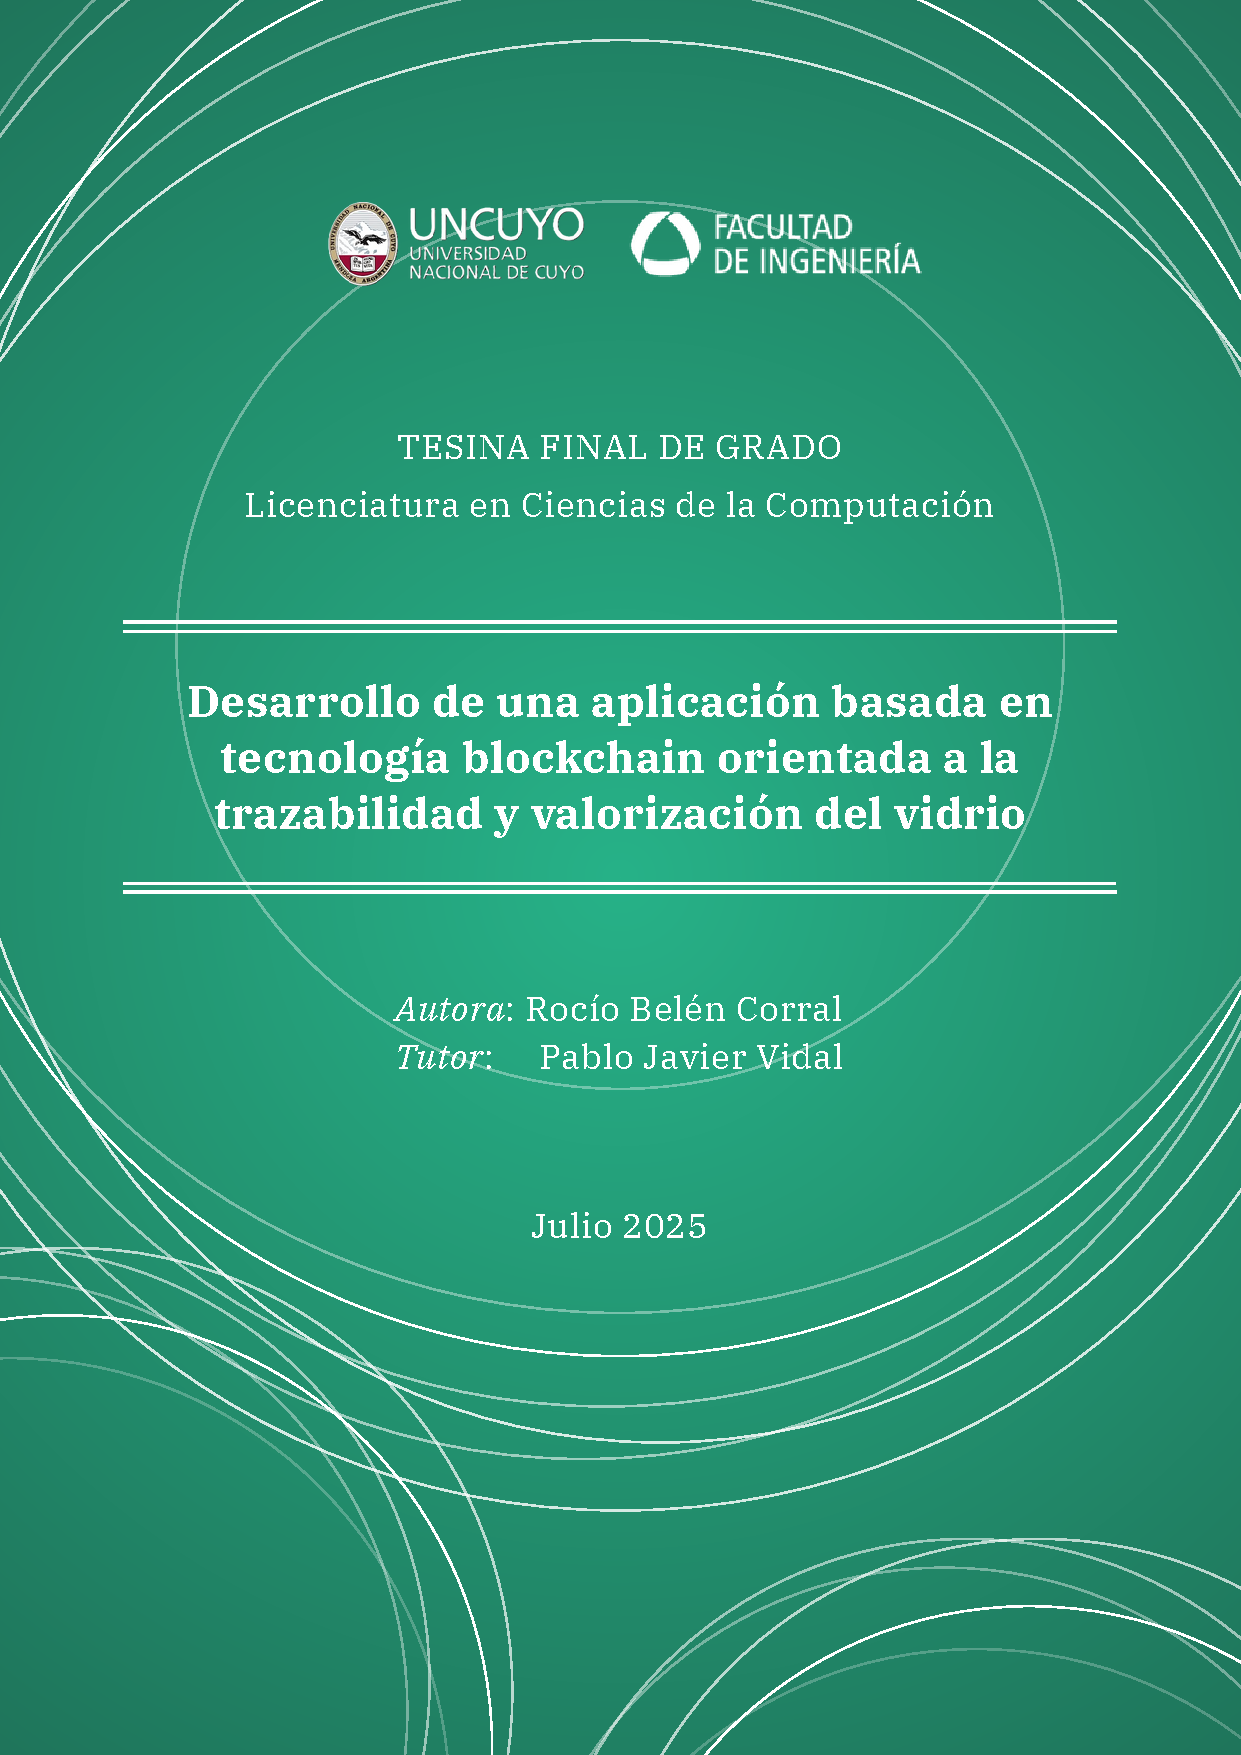
\includegraphics[width=\paperwidth,height=\paperheight,keepaspectratio]{Figures/Theme/Front-Page-Cover.pdf}%
        \vfill
      }%
    }%
  } %

\AddToShipoutPictureBG*{\BackgroundPicCover}

% TODO: change cover image
% ----------------------------------------
% Portada con cambio según LanguageOption
% ----------------------------------------
\newgeometry{
  top=1.5cm, bottom=1.77cm,
  left=2cm, right=1.5cm,
  bindingoffset=0cm
}
\begin{titlepage}
  \AddToShipoutPictureBG*{\BackgroundPicCover}
  \begingroup
    \plexsans %  Aplica IBM Plex Sans solo localmente

    % Color de texto según opción de portada
    \color{white}
    
    \vspace*{\fill}  % empuje vertical

  %     % ======= PORTADA EN ESPAÑOL =======
  %     {\noindent\bfseries\fontsize{12}{14}\selectfont TESIS DOCTORAL\par}
  %     \vspace{0.5cm}
  %     {\noindent\raggedright\itshape\fontsize{22}{24}\selectfont \titleesp\par}
  %     \vspace{2cm}

  %     \noindent
      
  %     \begin{minipage}[t]{0.4\textwidth}
  %       \raggedright
  %       \begin{tabbing}
  %         \hspace{4cm}\=\kill
  %         \textbf{\fontsize{12}{10}\selectfont AUTOR:}\> \GetFirstAuthor \\[0.3cm]
  %         \textbf{\fontsize{12}{10}\selectfont DIRECTORES:}\> \GetSupervisor   \\
  %                                             \> \GetCoSupervisor    \\
  %                                             \> \GetSecCoSupervisor
  %       \end{tabbing}
  %     \end{minipage}%
  %     \begin{minipage}[t]{0.45\textwidth}
  %       \vspace{2cm}
  %       \raggedleft
  %       {\fontsize{13}{16}\selectfont \the\year \par}
  %     \end{minipage}

    \vspace{1cm}
  \endgroup
\end{titlepage}
\restoregeometry
\MediaOptionLogicBlank

\include{Matter/01-Front-Page}

%%% Roman Numeration %%%
\pagenumbering{roman}

%%% Frase celebre %%%
\chapter*{} % Chapter* to appear without numeration

\begin{flushright}
    \textit{Être et Durer (Ser y durar)} \\
    \rule{5cm}{0.5pt} 
    % \\ Anónimo
\end{flushright}



%%% Acknowledgements %%%
\chapter*{Agradecimentos}

Comienzo este trabajo de tesis agradeciendo a todas las partes involucradas, a la facultad, profes, familia, amigos y hasta mis perros y gatos.

% TODO: add acknowledgements

\begin{block}[todo]
    \textit{Simplemente, tengo que redactar esto.}
\end{block}

\textit{Author: Rocío Belén Corral}
\textit{Date: \today}



%%% Abstract %%%
\thispagestyle{plain}
\chapter*{Resumen}

La trazabilidad permite identificar el origen, las etapas de producción y la distribución de bienes, facilitando la implementación de prácticas de economía circular, donde los residuos se reciclan o reutilizan en lugar de desecharse. En particular, es deseable poder realizar la trazabilidad del vidrio, dado que es un producto que puede ser reciclado o reinsertado en la cadena de suministro de diferentes formas sin perder su calidad.

Para proporcionar un nivel superior de transparencia, seguridad y eficiencia, los sistemas de trazabilidad están comenzando a hacer uso de la tecnología \textit{blockchain}. Esta tecnología permite crear registros inmutables y descentralizados, asegurando la integridad de la información y evitando manipulaciones externas. Además, brinda confianza a los consumidores al garantizar la autenticidad y calidad de los productos, mientras que también permite a las organizaciones que adoptan esta tecnología diferenciarse en el mercado, al demostrar su compromiso con la sostenibilidad y el respeto al medio ambiente.

En este trabajo se desarrolla un prototipo de sistema de trazabilidad de envases de vidrio basado en tecnología \textit{blockchain}, diseñado para registrar y verificar cada etapa de su ciclo de vida, desde la producción hasta su reintroducción en la cadena de valor, facilitando su valorización. Este desarrollo sigue un proceso de ingeniería de software bajo el modelo en V, el cual articula de manera rigurosa las fases de diseño, implementación y pruebas del sistema. A lo largo del presente trabajo, se profundiza en las etapas de análisis de requerimientos, diseño arquitectónico, implementación del prototipo y verificación exhaustiva de sus funcionalidades, con el fin de demostrar la viabilidad y los beneficios de aplicar \textit{blockchain} para una economía circular de vidrio sostenible y transparente.

\pdfbookmark[1]{Abstract}{abstract}
\chapter*{Abstract}

Traceability enables the identification of the origin and various stages of production and distribution of goods, facilitating the implementation of circular economy practices where waste is recycled or reused instead of discarded. In particular, it is desirable to achieve traceability for glass, as it is a product that can be recycled or reinserted into the supply chain in different ways without losing its quality.

To provide a superior level of transparency, security and efficiency, traceability systems are beginning to leverage blockchain technology. This technology allows for the creation of immutable and decentralized records, ensuring data integrity and preventing external manipulation. Furthermore, it fosters consumer confidence by guaranteeing product authenticity and quality, while also enabling organizations that adopt this technology to differentiate themselves in the marketplace by demonstrating their commitment to sustainability and environmental responsibility.

This work develops a prototype blockchain-based glass traceability system, designed to record and verify each stage of its lifecycle, from production to its reintroduction into the value chain, thus facilitating its valorization. This development follows a V-model software engineering process, which articulates the design, implementation and testing phases of the system. The stages of requirements analysis, architectural design, prototype implementation and exhaustive testing of its functionalities are detailed throughout the work, with the aim of demonstrating the viability and benefits of applying blockchain for a transparent and sustainable circular glass economy.


%%% Table of Contents, List of Figures and List of Tables %%%
\renewcommand{\contentsname}{Tabla de Contenidos}
\renewcommand{\listtablename}{Índice de Tablas}
\renewcommand{\listfigurename}{Índice de Figuras}

\bookmarktocentry\tableofcontents

\listoffigures

%%% Arabic Numeration %%%
\pagenumbering{arabic}

\listoftables

%%% Chapters of your thesis %%%%
\chapter[Introducción]{Introducción}
\label{cp:introduction}

\parindent0pt

Antes de comenzar con la descripción del trabajo realizado, es importante contextualizar el problema abordado y los objetivos que se pretende alcanzar. En este capítulo se introduce el contexto y la motivación del trabajo (Sección \ref{sec:motivation}), a continuación se detallan los objetivos (Sección \ref{sec:goals}) y, finalmente, se expone la estructura general del documento con el fin de guiar al lector a través del contenido desarrollado en los capítulos posteriores.

\section{Motivación}
\label{sec:motivation}

El mundo se enfrenta a un desafío ambiental sin precedentes: la gestión insostenible de los recursos naturales. La producción y consumo masivos de bienes generan un volumen creciente de residuos, lo que pone en riesgo la salud del planeta y el bienestar de las generaciones futuras \cite{IPCC2022, pelegri2021ipcc}. En este contexto, la transición hacia una economía circular se presenta como una solución prometedora para mitigar este impacto y construir un futuro más sostenible \cite{clima2022book}. Este modelo económico busca maximizar el valor de los recursos a lo largo de su ciclo de vida, minimizando el desperdicio y reintroduciendo los materiales en los sistemas de producción \cite{da2022economia, melendez2021economia}. Sin embargo, el principal desafío para lograr una economía circular radica en la falta de transparencia y trazabilidad dentro de las cadenas de suministro tradicionales.

Esta falta de visibilidad dificulta la capacidad para identificar oportunidades de reutilización y reciclaje, responsabilizar a las industrias por su impacto ambiental y empoderar a los consumidores para que tomen decisiones informadas. 

Investigaciones previas han explorado diversas tecnologías para mejorar la trazabilidad de la cadena de suministro, incluidos códigos de barras, identificación por radiofrecuencia (\gls{rfid}, \textit{Radio Frequency Identification}) y redes de sensores. Estas tecnologías ofrecen cierto nivel de capacidad de seguimiento; sin embargo, a menudo están limitadas por factores como la falta de estandarización, la fragmentación de información y la vulnerabilidad a manipulaciones \cite{schuitemaker2020product}.

En los últimos años, la tecnología \textit{blockchain} ha surgido como una solución prometedora para abordar estas limitaciones \cite{baralla2023waste, alnuaimi2023blockchain}. Sus características principales, como el registro de datos distribuido, la inmutabilidad y la transparencia, la convierten en una plataforma ideal para registrar y rastrear el movimiento de mercancías a lo largo de la cadena de suministro \cite{baralla2023waste}. Diversos estudios han explorado la aplicación de tecnología \textit{blockchain} para la trazabilidad de la cadena de suministro, demostrando su potencial para mejorar la transparencia y la responsabilidad dentro de estos sistemas. Ejemplos de estas aplicaciones incluyen la creación de un registro inmutable del origen de los productos para verificar su autenticidad y combatir la falsificación \cite{bulkowska2023implementation}, el rastreo de materiales a lo largo de la cadena de suministro para apoyar una economía circular \cite{baralla2023waste}, la optimización de la logística y la gestión de inventario mediante información en tiempo real \cite{signeblock2024} y la promoción de prácticas sostenibles al identificar productos con menor impacto ambiental \cite{bulkowska2023implementation}.

Las investigaciones realizadas hasta el momento reconocen el potencial de \textit{blockchain} para la trazabilidad de la cadena de suministro, pero muchas soluciones propuestas se enfocan únicamente en esta tecnología \cite{baralla2023waste, bulkowska2023implementation}, lo que limita su aplicabilidad en contextos donde se requiere la integración con sistemas de gestión tradicionales y tecnologías complementarias. Además, la mayoría de los estudios se centran en casos de uso específicos, como la industria alimentaria o farmacéutica, dejando una brecha significativa en la aplicación de \textit{blockchain} para mejorar la trazabilidad en otros sectores, como el reciclaje de vidrio.

En Latinoamérica, el vidrio representa el 5\% de los residuos sólidos urbanos \cite{cepal2021economia}, y solo el 20\% de este vidrio se recicla \cite{verallia2022whitebook}. La baja tasa de reciclaje de vidrio en la región se debe a la falta de infraestructura y sistemas de gestión adecuados, así como a la falta de conciencia y educación sobre la importancia del reciclaje. Mejorar la trazabilidad en la cadena de suministro del vidrio facilita su reciclaje, ayudando a promover una economía circular sostenible en la región. Al visibilizar el flujo de materiales, promover prácticas de reciclaje y facilitar la información y procesos a los usuarios, es posible reducir la generación de residuos, disminuir la extracción de materias primas vírgenes y fomentar la reutilización de materiales en la producción de nuevos envases de vidrio.

Considerando que la actividad económica principal de la provincia de Mendoza es la producción de vino, la cadena de suministro del vidrio adquiere una relevancia particular al proveer los envases para el embotellado. En este contexto, la falta de trazabilidad en dicha cadena es una problemática local y concreta cuya solución puede tener un impacto significativo en la sostenibilidad de la industria vitivinícola y, por extensión, en la economía regional. Por lo tanto, el presente trabajo se centra específicamente en la cadena de suministro y el reciclaje de los envases de vidrio, dada la importancia de este material reciclable en la economía circular y su papel en el desarrollo de la industria vitivinícola local.

Este trabajo tiene como objetivo desarrollar una solución de trazabilidad de envases de vidrio basada en la tecnología \textit{blockchain}, con el fin de mejorar la transparencia y la sostenibilidad a lo largo de todo su ciclo de vida. La solución propuesta busca abordar las limitaciones de las tecnologías existentes, al ofrecer una plataforma que permite a los actores de la cadena rastrear y verificar el origen, el movimiento y el estado de los envases. Para lograrlo, se plantea un enfoque abierto que integra la tecnología \textit{blockchain} con el Internet de las Cosas (\gls{iot}, \textit{Internet of Things}) y los sistemas de gestión tradicionales. Esta combinación permite aprovechar los datos en tiempo real provenientes de sensores para una visión más completa y confiable del producto, mientras que su compatibilidad con las prácticas comerciales existentes facilita su adopción. En última instancia, se espera que esta implementación represente un modelo factible y práctico para mejorar la trazabilidad de la cadena de suministro, contribuyendo a la transición hacia una economía circular sostenible. De este modo, se busca proporcionar una solución concreta y aplicable en el ecosistema mendocino, que a su vez pueda servir en un futuro como modelo para adaptarse a otras industrias y a una variedad de materiales reciclables.

\section{Objetivos}
\label{sec:goals}

El objetivo general de este trabajo consiste en hacer uso de \textit{blockchain} como tecnología de vanguardia para el desarrollo de una aplicación prototipo destinada a mejorar la trazabilidad en modelos de economía circular orientados al reciclaje de vidrio. A partir de este objetivo general, se definen los siguientes objetivos específicos:

\begin{itemize}
	\item \textbf{Objetivo 1}: entender los procesos de adopción de tecnologías tales como \textit{blockchain} y las capacidades actuales en la región para el uso de sistemas de trazabilidad.
	\item \textbf{Objetivo 2}: en lo referido a las Ciencias de la Computación, se busca desarrollar una aplicación prototipo funcional basada en tecnología \textit{blockchain}. Esto permitirá la trazabilidad transparente, segura y en tiempo real de la gestión de residuos, en particular el vidrio, desde su generación hasta su disposición final, con el fin de garantizar el cumplimiento normativo, mejorar la eficiencia operativa y aumentar la confianza entre todos los actores involucrados en el proceso.
\end{itemize}

\section{Estructura general del documento}
\label{sec:document-structure}

El presente documento se encuentra organizado en capítulos, cada uno de los cuales aborda un aspecto específico del trabajo realizado. En primer lugar, en el Capítulo \ref{cp:theoretical-framework}, se introduce el marco teórico, conceptos básicos relacionados con el problema y la tecnología utilizada, para luego continuar con un análisis de las soluciones existentes y los antecedentes académicos relevantes que contextualizan el trabajo. A continuación, en el Capítulo \ref{cp:methodology} se detalla la planeación del trabajo y la metodología adoptada. En el Capítulo \ref{cp:modelling} se describe el proceso de modelado de los requerimientos de la solución propuesta. En el Capítulo \ref{cp:design} se describe el diseño del sistema y en el Capítulo \ref{cp:implementation} se detalla su implementación. Posteriormente, en el Capítulo \ref{cp:testing} se presentan las pruebas realizadas y, finalmente, en el Capítulo \ref{cp:conclusions} se presentan las reflexiones obtenidas, los desafíos encontrados y las perspectivas futuras del proyecto.

Adicionalmente, al final del documento se incluyen una serie de apéndices como lectura opcional. El Apéndice \ref{cp:annex-content} incluye contenido externo como la demostración del prototipo, el código fuente y la documentación técnica del sistema. El Apéndice \ref{cp:verallia-interview} contiene una transcripción de la entrevista realizada a una empresa referente en la industria del vidrio en Mendoza. En el Apéndice \ref{cp:europe-trip} se presenta una minuta de un viaje de investigación realizado para estudiar sistemas de reciclaje y economía circular. El Apéndice \ref{cp:user-flows} incluye los flujos de usuario detallados para cada uno de los actores del sistema. El Apéndice \ref{cp:tests-execution-results} presenta los casos de prueba detallados y resultados obtenidos de cada etapa de la verificación del sistema. Finalmente, se incluye un glosario de términos específicos y abreviaturas que pueden resultar útiles para el lector a lo largo del documento.

\chapter[Marco Teórico]{Marco Teórico}
\label{cp:theoretical-framework}

\parindent0pt

% TODO: add references everywhere (except for introduction)

Este capítulo presenta los fundamentos teóricos que sirven de base para este trabajo. Se aborda la estructura y funcionamiento de las cadenas de bloques, destacando sus características de descentralización, transparencia e inmutabilidad, así como los mecanismos de consenso que garantizan su seguridad y eficiencia (Sección \ref{sec:blockchain}). Además, se analiza el rol de los contratos inteligentes como herramientas para automatizar procesos y gestionar la lógica de negocio en entornos descentralizados (Sección \ref{sec:smart-contracts}). Asimismo, este capítulo explora los principios de la economía circular, enfatizando su enfoque regenerativo y su capacidad para transformar las cadenas de suministro hacia modelos más sostenibles (Sección \ref{sec:circular-economy}). Se examinan las etapas del proceso de producción y reciclaje, con especial atención a la trazabilidad como habilitador para garantizar la transparencia y la eficiencia en una economía circular. Luego se incluye un análisis de la cadena de suministro del vidrio en el contexto mendocino, destacando su relevancia estratégica y los desafíos asociados a su implementación en un modelo circular. Finalmente, se explora el estado del arte de la tecnología \textit{blockchain} en la economía circular, identificando las tendencias actuales y las oportunidades de mejora en la trazabilidad y sostenibilidad de la cadena de suministro del vidrio (Sección \ref{sec:related-work}).

\section{Blockchain}
\label{sec:blockchain}

Blockchain es una tecnología emergente y potencialmente disruptiva que permite registrar información de forma segura, transparente y sin intermediarios. Esta tecnología está siendo aplicada para diversos casos de uso y ha sido objeto de creciente atención tanto en el ámbito empresarial como académico desde su aparición en 2008 \cite{satoshi2008bitcoin}. La primera y más famosa aplicación de blockchain es Bitcoin. Su inventor anónimo, Satoshi Nakamoto, lanzó Bitcoin en 2008 durante la crisis financiera mundial con el objetivo de crear un nuevo tipo de moneda digital confiable fuera del control de gobiernos, bancos y otras instituciones financieras tradicionales \cite{satoshi2008bitcoin}. Desde entonces, la tecnología blockchain ha sido adoptada en diversos sectores. En el ámbito financiero, se utiliza como un libro contable digital para facilitar transferencias de valor entre pares, sin bancos ni entidades intermediarias \cite{bulkowska2023implementation}. En logística y cadenas de suministro, se aplica para mejorar la trazabilidad, transparencia y eficiencia de los procesos productivos \cite{rejeb2023role}.

La tecnología \textit{blockchain}, o cadena de bloques, sirve para registrar información digital de manera segura, transparente e inmutable. Es relevante comprender los motivos de su surgimiento como una tecnología disruptiva en los últimos años, antes de introducir su estructura y funcionamiento \cite{pending}.

Para entender la necesidad e impacto de la tecnología blockchain, primero es necesario analizar la arquitectura predominante de Internet hasta la actualidad, basada tradicionalmente en un modelo centralizado cliente-servidor. En este esquema, los datos son almacenados en servidores administrados por proveedores, quienes actúan como intermediarios de confianza entre los clientes o usuarios. Aunque este modelo ha facilitado el intercambio de información a escala masiva, también trae aparejados ciertos problemas de confianza, seguridad y privacidad \cite{gunawan2024review}. La centralización implica que los usuarios ceden el control y gestión de sus datos a terceros, lo que puede derivar en una dependencia significativa de estas entidades para la integridad y disponibilidad de la información. Ejemplos de esto incluyen la exposición de datos personales privados en ciber-ataques, la interrupción de servicios por fallas en servidores centrales o la censura de contenido por decisiones unilaterales de las plataformas \cite{gunawan2024review}. Por ejemplo, cuando el servidor de Whatsapp deja de funcionar, los usuarios no pueden utilizar la aplicación para comunicarse hasta que el proveedor vuelva a hacerlo funcionar. Otro ejemplo, es cuando un proveedor sufre un ciber-ataque y se filtran contraseñas de los usuarios, quienes no tienen conocimiento de las vulnerabilidades que puede tener el proveedor, pero dependen de su servicio \cite{pending}.

Ante los desafíos de confianza e integridad en los sistemas centralizados, la tecnología blockchain emergió en 2008 como una solución disruptiva. Concebida inicialmente como la base del sistema de criptomonedas Bitcoin \cite{satoshi2008bitcoin}, la blockchain actúa como un libro de contabilidad digital descentralizado que facilita transferencias de valor entre pares sin la necesidad de intermediarios. Esta funcionalidad revolucionaria rápidamente demostró un potencial significativo más allá del ámbito financiero, posicionando a la tecnología blockchain como una herramienta para abordar problemas de confianza, transparencia e inmutabilidad en la gestión de datos \cite{bulkowska2023implementation}. Su arquitectura permite el registro de información de manera distribuida, eliminando la dependencia de proveedores centralizados y habilitando la interacción directa entre múltiples partes \cite{bulkowska2023implementation}.

\begin{figure}[!tb] 
    \centering
    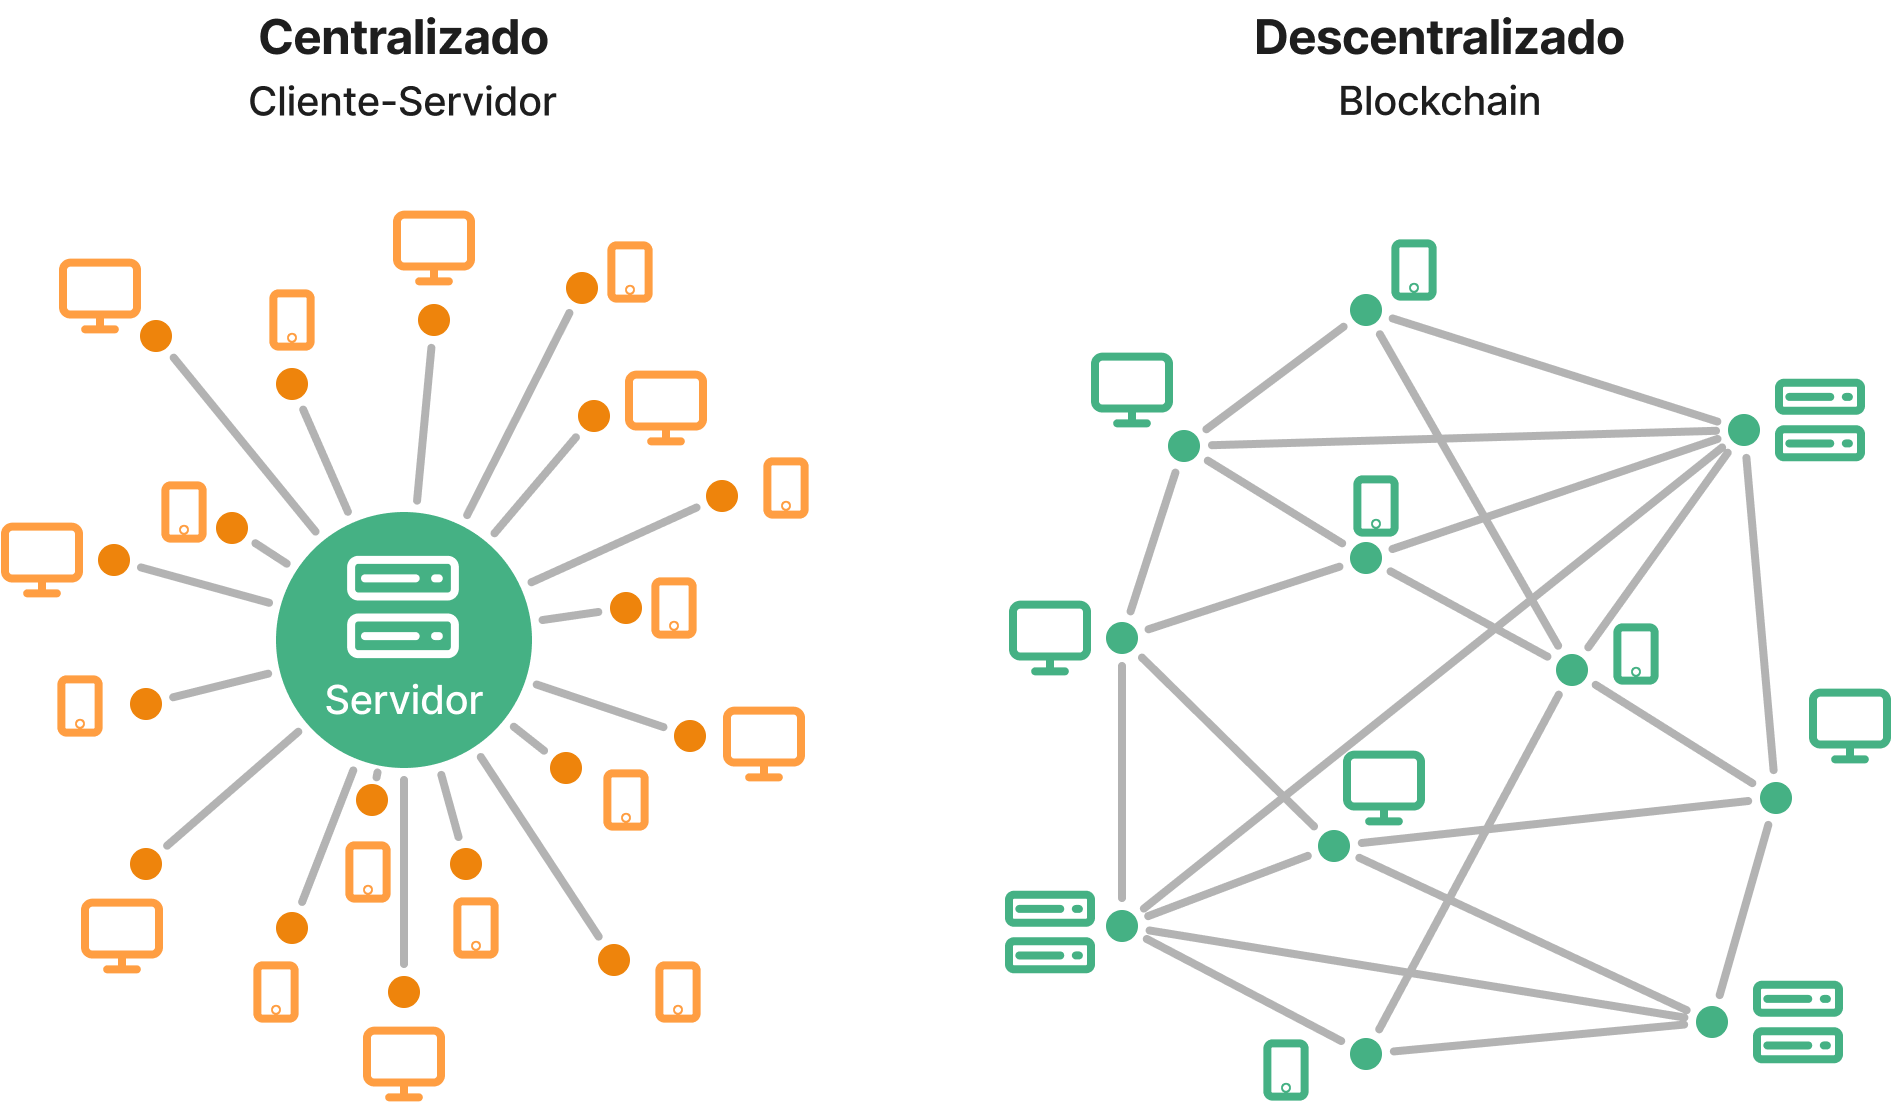
\includegraphics[width=0.8\textwidth]{Figures/client-server-vs-p2p.png}
    \caption{Comparación entre el modelo cliente-servidor y el modelo distribuido de blockchain}
    \label{fig:web-architecture}
\end{figure}

A diferencia de lo que suele suponerse, blockchain no se basa en tecnologías radicalmente nuevas, sino que integra de forma innovadora principios existentes de la computación y las matemáticas. Combina conceptos de criptografía (para asegurar la información), redes distribuidas (para la replicación de los datos) y teoría de juegos e incentivos (para coordinar el comportamiento de los participantes y garantizar la seguridad de los datos) \cite{sunny2022systematic, bulkowska2023implementation}. Esta integración produce un sistema seguro, transparente y resistente a manipulaciones, características difíciles de lograr en modelos centralizados. De esta manera, blockchain impulsa un nuevo paradigma donde el registro de la información es gestionado colectivamente, lo que permite transacciones y acuerdos entre pares sin depender de un tercero de confianza centralizado.

A continuación, se explorará en detalle la estructura y funcionamiento de la tecnología blockchain, sus características distintivas, los mecanismos de consenso que garantizan su seguridad y el papel de los contratos inteligentes como herramientas para la automatización de procesos. Además, se analizarán las ventajas y desafíos asociados a su implementación, así como su potencial de uso más allá del ámbito financiero.

\subsection{Estructura de una Blockchain}

La tecnología \textit{blockchain}, o cadena de bloques, es una estructura de datos distribuida y descentralizada donde la información se organiza en transacciones agrupadas en bloques enlazados criptográficamente. Cada bloque posee un código único, conocido como \textit{hash del bloque}, que lo identifica y sirve para enlazarlo al bloque posterior. El hash de cada bloque se genera a partir de su contenido y del hash del bloque anterior, creando así una cadena continua de bloques interconectados \cite{tripathi2023comprehensive}. En la Figura \ref{fig:blockchain-basic} se ilustra la estructura simplificada de una blockchain, donde cada bloque incluye el hash del bloque anterior, formando una cadena de bloques interconectados.

\begin{figure}[!tb]
    \centering
    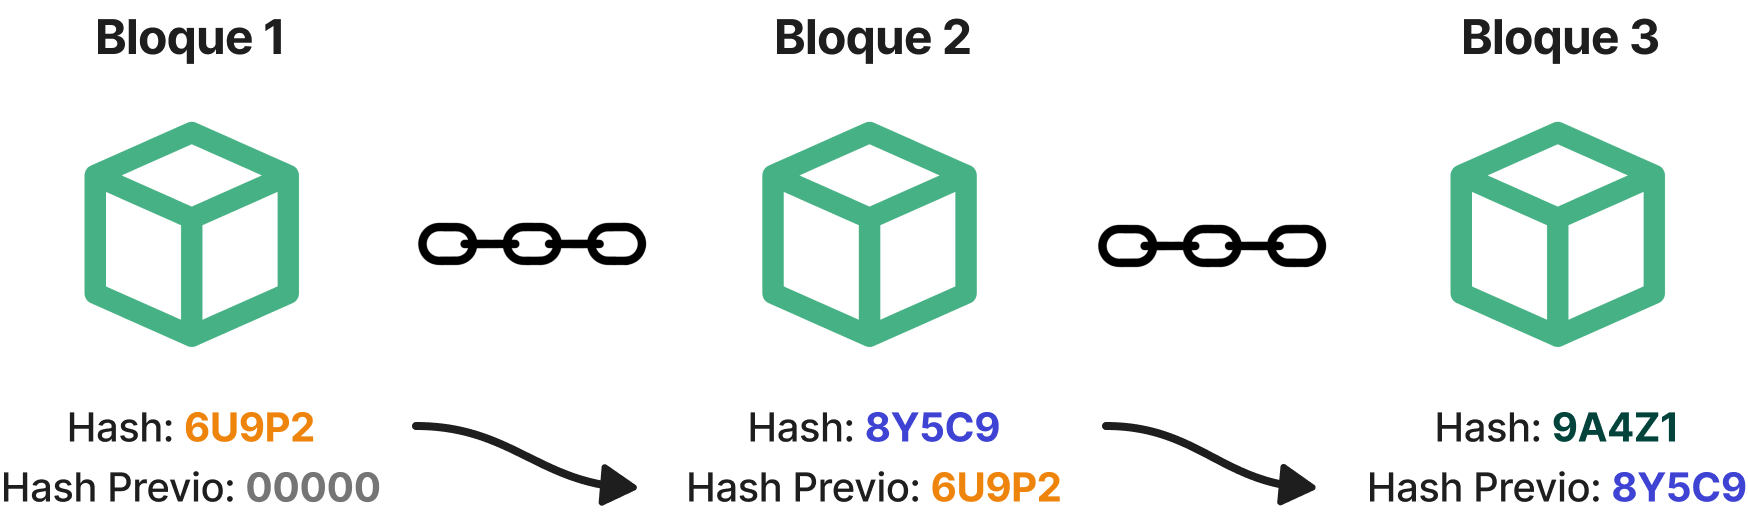
\includegraphics[width=0.8\textwidth]{Figures/blockchain-basic.png}
    \caption{Estructura básica de una cadena de bloques}
    \label{fig:blockchain-basic}
\end{figure}

Cada bloque de la cadena consta de un encabezado y un cuerpo \cite{tripathi2023comprehensive}. El cuerpo guarda la lista de transacciones, mientras que el encabezado contiene metadatos (que pueden variar en cada implementación). Entre los metadatos más relevantes se encuentran el código único del bloque anterior, una marca de tiempo, y el código que identifica unívocamente al bloque actual. En la Figura \ref{fig:block-structure} se puede observar un esquema del contenido de un bloque de la cadena.

\begin{figure}[!tb]
    \centering
    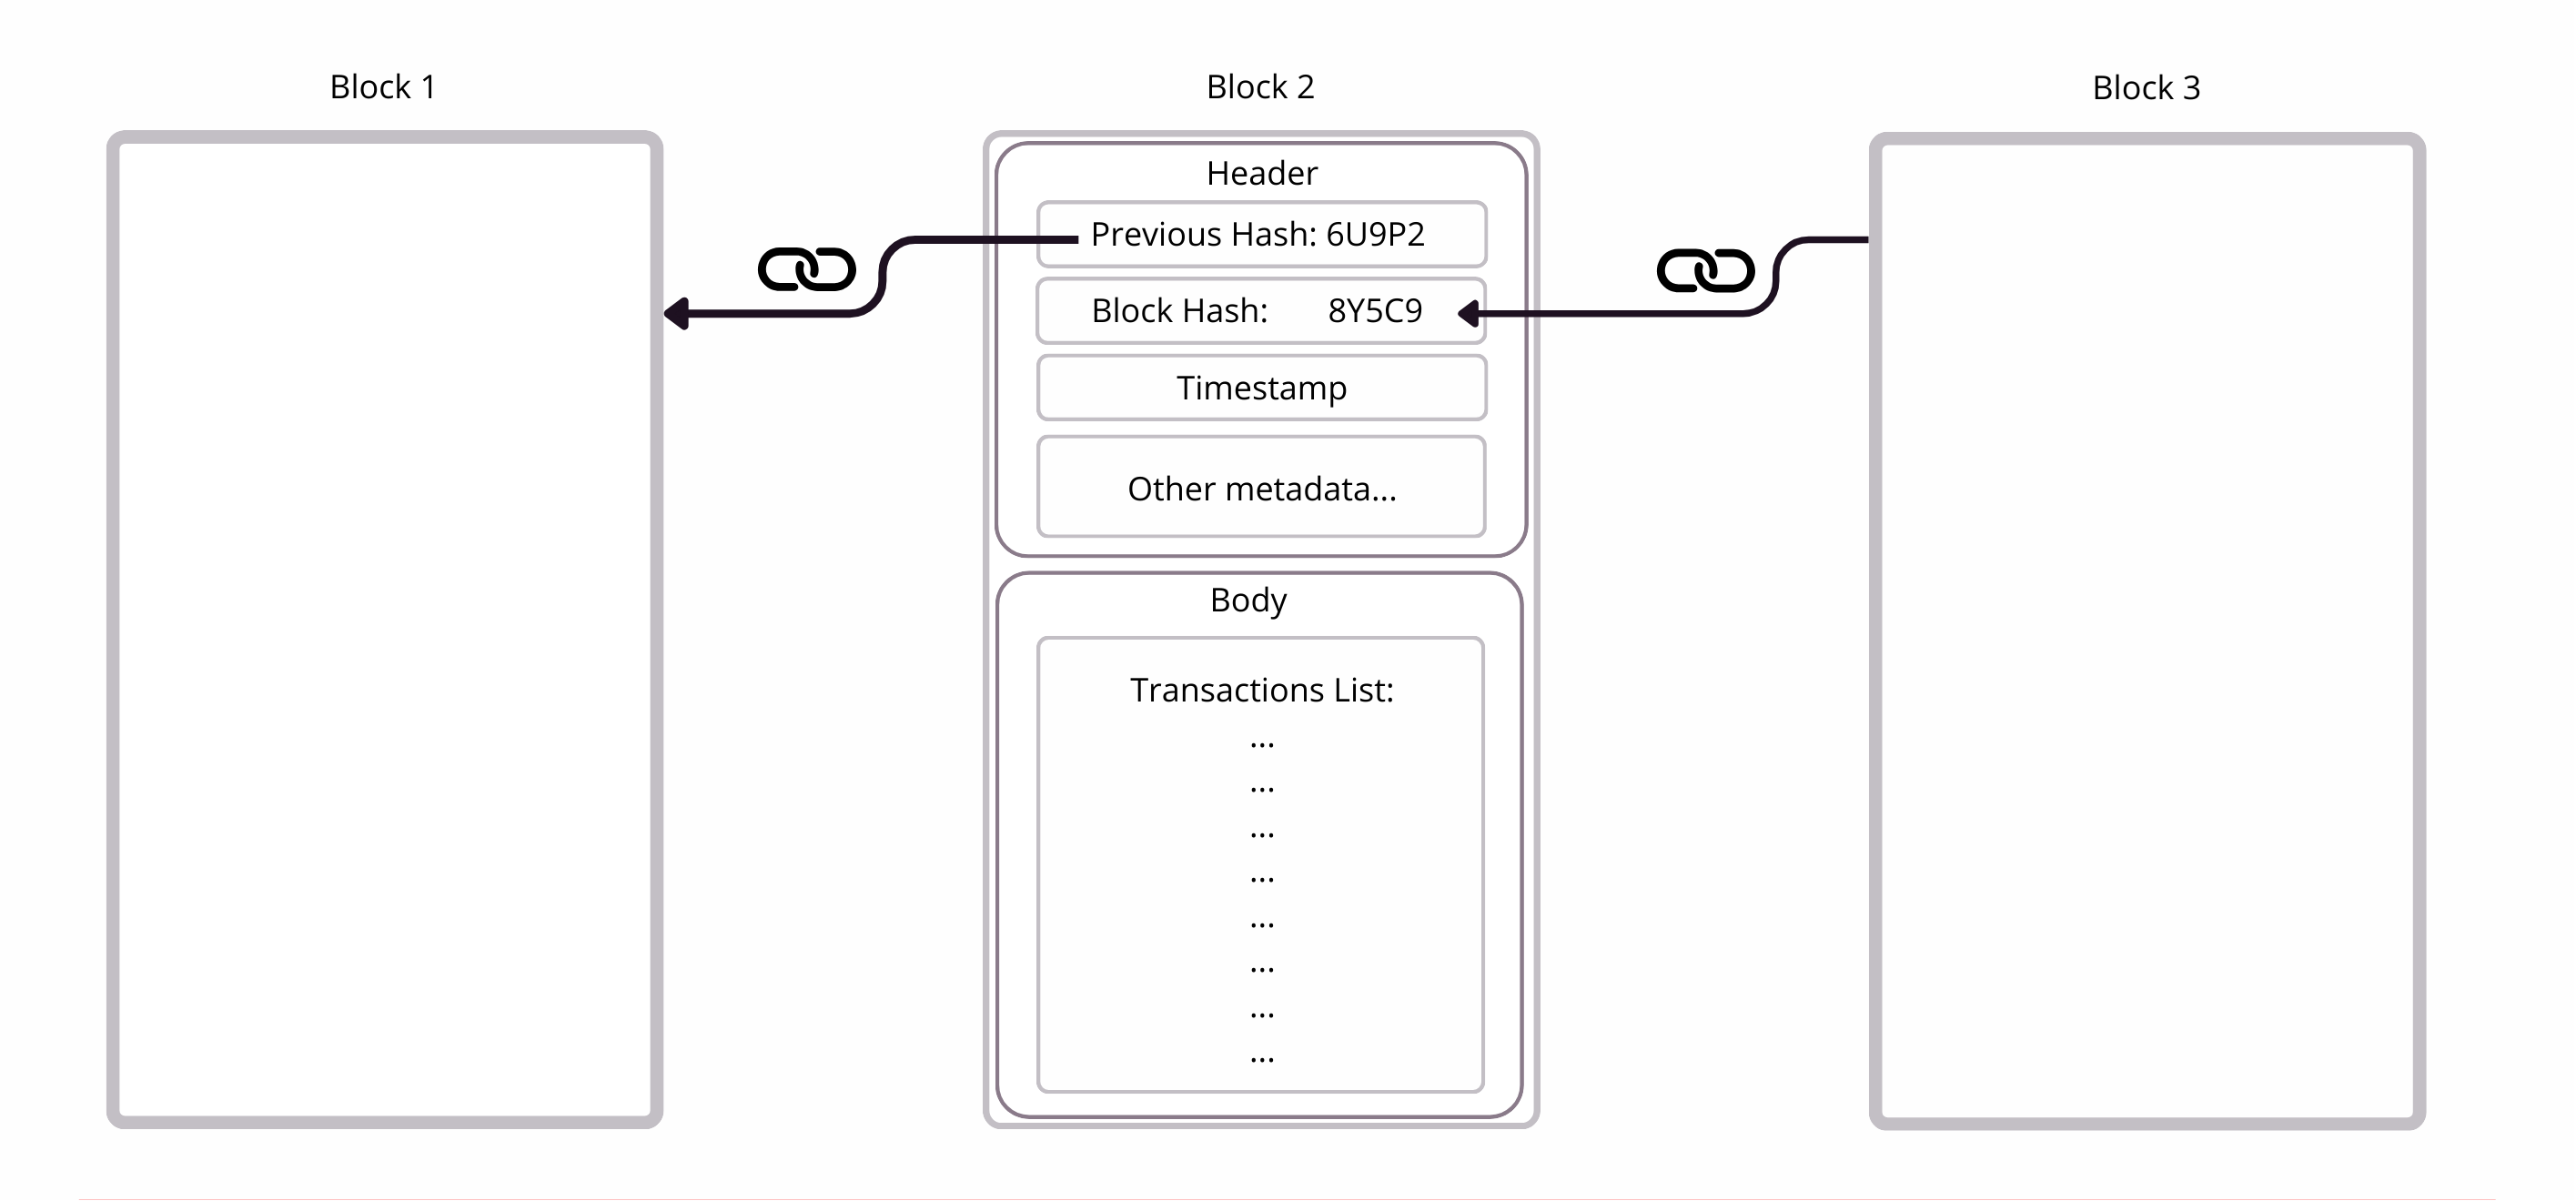
\includegraphics[width=0.8\textwidth]{Figures/block-structure.png}
    \caption{Contenido de un bloque en una cadena de bloques}
    \label{fig:block-structure}
\end{figure}

El hash del bloque se calcula usando funciones hash criptográficas, que son algoritmos matemáticos que transforman datos de entrada en una cadena de caracteres de longitud fija. Los códigos hash tienen la propiedad de ser rápidos de calcular, difíciles de revertir (matemáticamente imposible hacerles ingeniería inversa) y únicos para cada conjunto de datos (cualquier cambio en el contenido del bloque generará un código hash completamente diferente) \cite{pending}. Estas características permiten verificar la integridad de los datos almacenados en la cadena, ya que el código hash de un bloque se puede recalcular en cualquier momento y comparar con el código almacenado en la cadena. Si los códigos coinciden, se puede confiar en que los datos no han sido alterados; si no coinciden, se ha producido una modificación no autorizada en el contenido del bloque \cite{pending}. En la Figura \ref{fig:hash-example} se puede ver un ejemplo de los códigos generados usando un algoritmo hash a partir de dos cadenas parecidas, donde se observa que incluso un cambio mínimo en el contenido produce un hash completamente diferente. 

\begin{figure}[!tb]
    \centering
    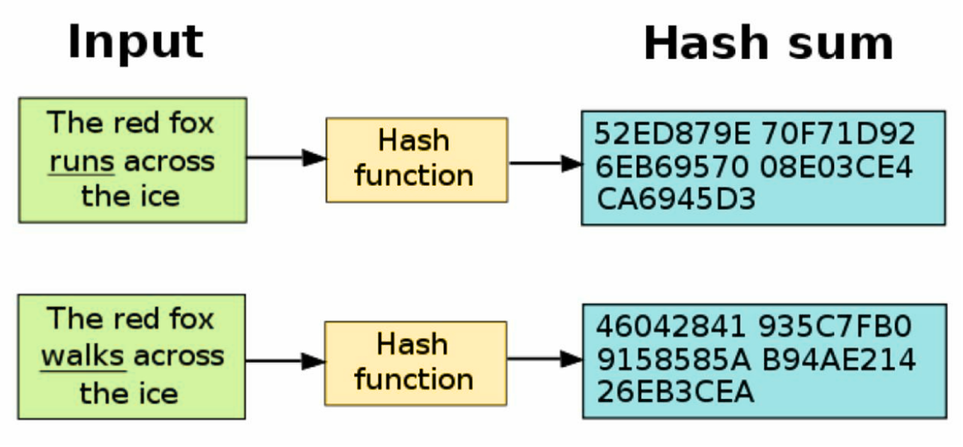
\includegraphics[width=0.8\textwidth]{Figures/hash-example.png}
    \caption{Ejemplo de códigos hash generados a partir de cadenas de texto}
    \label{fig:hash-example}
\end{figure}

La interconexión criptográfica entre los bloques confiere a blockchain su característica de inmutabilidad. Una vez que un bloque es añadido a la cadena, su hash se calcula a partir de su contenido y el hash del bloque anterior. Cualquier intento de alterar el contenido del bloque invalidaría este hash y, por ende, los hashes de todos los bloques subsiguientes, rompiendo la integridad criptográfica de la cadena. Este mecanismo permite la detección de cualquier intento de manipulación y la preservación de la integridad histórica del registro \cite{bulkowska2023implementation}. 

Como ya se mencionó, la blockchain es una estructura de datos distribuida y descentralizada. La naturaleza distribuida de la blockchain implica que la información no se encuentra almacenada en un único servidor, sino que está distribuida en una red de computadoras interconectadas (conocidas como nodos) y cada nodo de la red mantiene una copia completa y actualizada del registro (de toda la cadena de bloques). Esto asegura su transparencia y resiliencia al no depender de un servidor central \cite{bulkowska2023implementation} propenso a ataques maliciosos y puntos únicos de fallo. Por su parte, la descentralización implica la ausencia de una autoridad central, de modo que la validación y adición de nuevos bloques se rige por un \textit{mecanismo de consenso} entre todos los nodos participantes de la red. 

Precisamente en este marco, los mecanismos de consenso son algoritmos o una serie de reglas que se definen en una red distribuida para que todos los nodos (que en este caso deben guardar exactamente la misma cadena de bloques) se pongan de acuerdo sobre qué información es correcta y válida. Sin un mecanismo de consenso, la red sería vulnerable a ataques por parte de nodos maliciosos que esparzan información inválida por la red con fines de beneficio propio, pudiendo perjudicar al resto de la red. Por ejemplo, en la red Bitcoin, cada transacción representa una transferencia de fondos entre cuentas; un nodo podría difundir transacciones al resto de la red registrando que cientos de usuarios le transfirieron fondos a una cuenta en específico, si el mecanismo de consenso no definiera reglas para validar el origen legítimo de cada transacción, este nodo malicioso podría robar los fondos de los demás usuarios para beneficio exclusivo de la persona que controla ese nodo.

Cada nodo de la red blockchain ejecuta un mismo programa computacional (software) que codifica las reglas del mecanismo de consenso, definiendo cómo crear transacciones y bloques válidos, transmitirlos a la red y comprobar la validez de una transacción o bloque recibido de otro nodo antes de agregarlo a su copia local de la cadena (o descartarlo si no es válido). Para unirse a la red, un nuevo nodo descarga una copia completa de la cadena de bloques existente, lo que le confiere una visión completa del historial de transacciones y el estado actual de la cadena \cite{bulkowska2023implementation}. Posteriormente, el nodo comienza a ejecutar el software del mecanismo de consenso. A partir de entonces, el nodo puede generar nuevas transacciones y transmitirlas a la red para ser recibidas por los demás nodos. Asimismo, el nodo recibe transacciones de otros nodos y las valida mediante el mecanismo de consenso antes de añadirlas a un bloque en su copia local de la cadena \cite{bulkowska2023implementation}.

La combinación de estas características, el encadenamiento criptográfico de bloques, la red descentralizada y el mecanismo de consenso, es lo que le permite a la blockchain garantizar la integridad e inmutabilidad de la información. Esto se debe a que cualquier alteración maliciosa en un bloque de la cadena modificaría su hash y rompería la consistencia posterior de la cadena, forzando a cada nodo de la red descentralizada a rechazar el bloque modificado. En consecuencia, para recuperar la consistencia de la cadena, sería necesario modificar los hashes de todos los bloques posteriores, lo que sería un proceso computacionalmente costoso y fácilmente detectable por el resto de la red.

En la actualidad, existen múltiples y variados algoritmos de consenso que definen distintas formas de generar un bloque válido (desde un nodo) y comprobar la validez del bloque (recibido desde otro nodo). Cada mecanismo de consenso utiliza distintas técnicas de teoría de juegos e incentivos con el objetivo de incentivar a que se unan nuevos nodos a la red (obteniendo ganancias) y desincentivar que un nodo actúe de manera maliciosa para obtener un beneficio individual. Esta combinación se logra mediante esquemas donde la penalización o pérdida generada por un comportamiento malicioso supere con creces las ganancias que se puedan obtener comportándose de forma maliciosa. Ejemplos prominentes de la diversidad de algoritmos de consenso incluyen la Prueba de Trabajo (PoW), la Prueba de Participación (PoS) y la Prueba de Autoridad (PoA), cada uno con características particulares.

El mecanismo de Prueba de Trabajo (\textit{PoW}, por sus siglas en inglés) es uno de los algoritmos de consenso más conocidos y el primero introducido en las redes blockchain por su implementación en Bitcoin \cite{satoshi2008bitcoin}. En PoW, todos los nodos (conocidos como ``mineros`` en este contexto) compiten para resolver un problema matemático complejo que requiere una gran capacidad computacional. El primer nodo que logra resolver este problema matemático valida la transacción y crea el nuevo bloque incluyendo la solución en su encabezado. El resto de nodos recibe el bloque y comprueba que el problema haya sido resuelto correctamente. El nodo que resuelve el reto recibe una compensación en Bitcoin como incentivo por aportar un bloque válido a la red. La desventaja de este algoritmo de consenso es que implica un alto costo energético debido a la carga computacional requerida para resolver el problema \cite{pending}.

Otro mecanismo ampliamente utilizado es Prueba de Participación (\textit{PoS}, por sus siglas en inglés), a diferencia de PoW, no requiere de una alta capacidad computacional para la creación de bloques. En PoS, los nodos (conocidos como validadores) ``apuestan`` una cantidad de las criptomonedas como garantía de su buen comportamiento. Para generar un bloque válido, el protocolo selecciona pseudo-aleatoriamente un validador para generar el siguiente bloque, con una probabilidad de selección proporcional a la cantidad de criptomonedas que ha apostado. Una vez que el validador seleccionado crea un bloque y lo transmite a la red, los demás nodos validadores de la red simplemente comprueban que el bloque cumpla con las reglas de negocio del protocolo. Si un validador actúa de manera maliciosa, puede perder parte o la totalidad de su participación (proceso conocido como ``slashing``). La principal ventaja del PoS es su eficiencia energética significativamente mayor en comparación con PoW, ya que no se requiere una minería intensiva. Además, puede ofrecer mayor escalabilidad y tarifas de transacción más bajas. Ethereum es un ejemplo de protocolo blockchain que fue implementado originalmente con PoW, pero que se actualizó para utilizar PoS debido a estas ventajas. Sin embargo, una desventaja potencial es el riesgo de centralización si la mayoría de la participación se acumula en pocos nodos, lo que podría darles un control desproporcionado sobre la red.

La Prueba de Autoridad (\textit{PoA}, por sus siglas en inglés) es otro mecanismo de consenso donde la validación de bloques se basa en la identidad y reputación de un conjunto pre-aprobado de validadores. Para generar un bloque válido, el protocolo elige una autoridad designada (del conjunto de validadores aprobados y de confianza) que tiene el derecho exclusivo de crear y firmar el nuevo bloque. Para verificar que un bloque es válido, los demás nodos de la red simplemente comprueban la firma digital del validador que lo propuso y que el bloque cumple con las reglas del protocolo. La principal ventaja del PoA es su alta velocidad de transacción, ya que solo un número limitado de validadores de confianza necesita llegar a un consenso. Esto lo hace ideal para redes privadas o consorcios donde la confianza entre los participantes ya existe. Sin embargo, esta misma es su mayor desventaja, ya que la seguridad y el control de la red dependen de un pequeño grupo de entidades conocidas, lo que va en contra del principio de descentralización de muchas blockchains públicas.

Cada uno de los mecanismos mencionados ofrece distintos niveles de eficiencia de procesamiento, seguridad y descentralización. Durante la validación del bloque, se verifican múltiples aspectos en común en cualquiera de estos mecanismos: la correcta correspondencia del hash del bloque anterior con el almacenado en el encabezado del nuevo bloque, la validez de las transacciones de acuerdo a la lógica de negocios propia del protocolo blockchain, y que el hash del bloque propuesto haya sido generado correctamente a partir de la totalidad de su contenido.

Todo algoritmo de consenso debe asegurar que el costo de modificar un bloque de forma fraudulenta supere significativamente el beneficio potencial derivado de dicha acción \cite{satoshi2008bitcoin}. Esta característica garantiza que la red se mantenga segura y resistente a ataques \cite{buterin2013ethereum}. En el caso de Bitcoin, por ejemplo, el algoritmo de consenso Proof of Work (PoW) exige que los nodos realicen cálculos computacionales intensivos para generar nuevos bloques válidos. Aunque la validación de un bloque es de complejidad constante, la alteración de un bloque ya existente implicaría la necesidad de recalcular no solo dicho bloque, sino también todos los bloques subsiguientes. Esto convierte la modificación en un proceso extremadamente costoso en términos de recursos computacionales y energía, lo cual, sumado al rechazo de la red hacia cualquier cadena alterada, desincentiva eficazmente los intentos de manipulación \cite{satoshi2008bitcoin}.

En síntesis, la robustez de una blockchain reside en la interconexión sinérgica de sus componentes: el encadenamiento criptográfico, la red distribuida y el mecanismo de consenso. No es un único elemento el que garantiza su seguridad, sino la forma en que estos principios interactúan constantemente. Los mecanismos de consenso, en particular, son los encargados de arbitrar la creación de nuevos bloques de forma segura, resolviendo el problema de la confianza en un entorno descentralizado. A su vez, el encadenamiento criptográfico asegura que la integridad de un bloque dependa del anterior, haciendo que cualquier intento de manipulación sea computacionalmente costoso y fácilmente detectable por el resto de la red.

A continuación, se detalla cómo estos elementos se articulan en la práctica para permitir un registro de transacciones seguro y transparente. A través de un proceso iterativo de validación, los nodos de la red trabajan de forma coordinada para generar, verificar y distribuir nuevos bloques, conformando un ciclo de vida que asegura la consistencia y la inmutabilidad del registro global de transacciones.

\subsection{Funcionamiento de una Blockchain}

Teniendo conocimiento de los elementos fundamentales que conforman una blockchain, es posible analizar cómo interactúan para registrar y validar transacciones de manera coordinada en un entorno descentralizado. Este proceso, que combina principios criptográficos, distribución de datos y reglas de consenso, se desarrolla de forma secuencial y repetitiva, asegurando que cada bloque añadido a la cadena preserve la integridad del registro global de transacciones. En la Figura \ref{fig:blockchain-working} se presenta un esquema ilustrativo con los pasos del proceso de incorporación de una nueva transacción y su respectivo bloque en una blockchain. 

\begin{figure}[!tb]
    \centering
    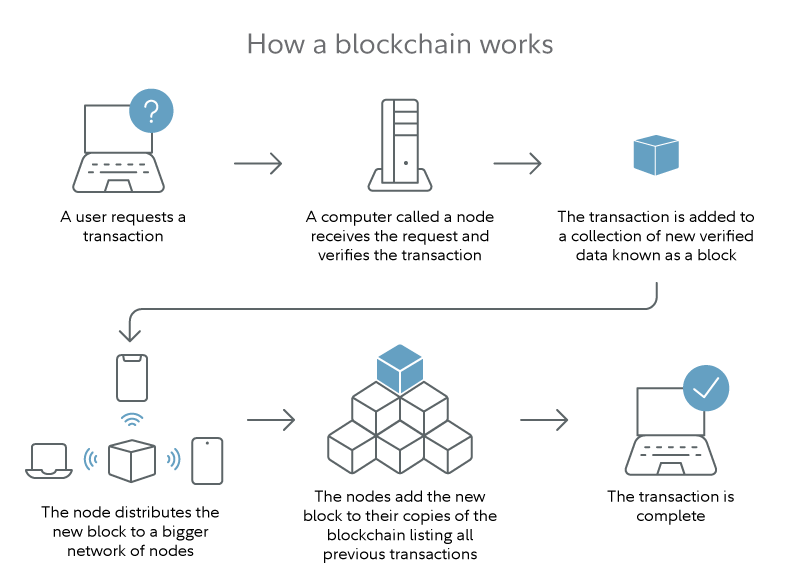
\includegraphics[width=0.8\textwidth]{Figures/block-creation.png}
    \caption{Creación de una transacción y un bloque en una blockchain}
    \label{fig:blockchain-working}
\end{figure}

El proceso de incorporación de una nueva transacción y su respectivo bloque en una blockchain se desarrolla a través de los siguientes pasos:

\begin{enumerate}
    \item Un nodo de la red crea y firma una nueva transacción con su clave privada (la firma criptográfica garantiza la autenticidad de la transacción)
    \item La transacción se propaga a través de la red distribuida, donde es recibida por cada nodo participante.
    \item Cada nodo valida la transacción individualmente, verificando la firma del remitente y asegurándose de que la transacción cumple con la lógica de negocios propia del protocolo blockchain (por ejemplo, en Bitcoin, que el remitente cuente con los fondos a transferir). Una vez validada, la transacción se añade a un \textit{pool} de transacciones pendientes. En caso de ser inválida, simplemente se ignora y se descarta. 
    \item Cuando un nodo tiene suficiente cantidad de transacciones en su \textit{pool}, procede a seleccionar un conjunto de transacciones pendientes del \textit{pool} para formar un nuevo bloque. Este bloque incluye las transacciones seleccionadas, el hash del bloque anterior y otros metadatos (como la marca de tiempo y un \textit{nonce} para PoW). Luego, el nodo calcula el hash de este nuevo bloque y, según el algoritmo de consenso, realiza el trabajo necesario para garantizar que sea válido. En el caso de PoW, esto implica resolver un problema criptográfico que requiere una cantidad significativa de potencia computacional. En PoS, el nodo debe demostrar que posee una cantidad suficiente de fondos para participar en la validación del bloque.
    \item Una vez que el nodo ha validado el nuevo bloque (o ``minado`` en PoW), lo difunde a la red. Los demás nodos reciben este bloque y verifican su validez (incluyendo el hash, las transacciones y la prueba de trabajo/participación). Si el bloque es válido, cada nodo lo añade a su copia local de la cadena de bloques y descarta de su \textit{pool} de pendientes las transacciones incluidas en el bloque. Si el bloque es inválido, es rechazado por cada nodo y no se añade a la cadena.
\end{enumerate}

De esta manera, la cadena de bloques se actualiza de forma continua y descentralizada, asegurando que todos los nodos de la red mantengan una copia idéntica y consistente del registro de transacciones. En su concepción inicial, las transacciones en un bloque se asociaban comúnmente a movimientos financieros \cite{satoshi2008bitcoin}, pero la flexibilidad inherente de la tecnología blockchain permite que los bloques contengan cualquier tipo de información estructurada \cite{bartolomeo2020introduccion}. Esta versatilidad ha sido el motor para el desarrollo de aplicaciones más complejas, destacando entre ellas los contratos inteligentes \cite{sunny2022systematic}, que permiten almacenar programas computacionales en la blockchain, habilitando la automatización segura de procesos como la trazabilidad, la certificación de origen o la valorización de materiales reciclados.

\subsection{Contratos Inteligentes}
\label{sec:smart-contracts}

A mediados de la década de 1990, cuando el comercio electrónico comenzaba a expandirse y se buscaban mecanismos seguros para realizar transacciones entre personas sin relación previa y sin confianza mutua, el criptógrafo y jurista Nick Szabo propuso el concepto de contrato inteligente \cite{pending}. Lo definió como un protocolo informático diseñado para ejecutar de forma automática los términos de un acuerdo, reduciendo la necesidad de intermediarios humanos y de documentos legales tradicionales.

En su concepción original, estos contratos no dependían necesariamente de blockchain. Sin embargo, la aparición de esta tecnología a partir de Bitcoin en 2008 y, especialmente, la introducción de Ethereum en 2015, proporcionó por primera vez una infraestructura distribuida, segura e inmutable capaz de materializar la idea de Szabo. Hoy, un contrato inteligente es un programa almacenado en una blockchain que se activa y ejecuta automáticamente cuando se cumplen condiciones predefinidas, garantizando que los acuerdos se lleven a cabo tal como fueron codificados, sin intervención de terceros de confianza \cite{bulkowska2023implementation}. Su función principal es automatizar procesos en entornos descentralizados, reduciendo la dependencia de intermediarios humanos \cite{verma2023overview} y mejorando la eficiencia operativa en múltiples sectores \cite{sunny2022systematic}.

Para codificar las reglas de un contrato inteligente, se emplean lenguajes de programación específicos adaptados a cada plataforma blockchain \cite{bartolomeo2020introduccion}. Un ejemplo prominente es \textit{Solidity} \cite{taherdoost2023smart}, utilizado en Ethereum, un lenguaje orientado a objetos diseñado específicamente para esta finalidad. Los contratos programados en Solidity pueden interactuar entre sí y con el estado global de la blockchain, habilitando la creación de aplicaciones descentralizadas (conocidas también como \textit{dApps}, por sus siglas en inglés) que operan de forma autónoma y sin intermediarios en la red \cite{buterin2013ethereum}.

Un contrato inteligente se concibe como un conjunto de reglas y lógica de negocio codificadas. Cada contrato posee un código (las reglas, por ejemplo, en Solidity) y un estado (la información dinámica almacenada en la blockchain) \cite{buterin2013ethereum}. El código del contrato es inmutable una vez desplegado en la blockchain mediante una transacción, garantizando la permanencia de las reglas establecidas. Su estado, sin embargo, puede evolucionar a medida que se interactúa con el contrato a través de transacciones. Es importante destacar que, si bien se describen como auto-ejecutables por su automatismo al cumplir condiciones, su ejecución es llevada a cabo por los nodos de la red que validan las transacciones e integran los cambios de estado en la cadena \cite{buterin2013ethereum}. Tanto el código como el estado del contrato se almacenan en la blockchain, asegurando su transparencia y disponibilidad pública. Por ejemplo, un contrato inteligente podría gestionar un sistema de votación, donde los participantes envían sus votos y el contrato contabiliza automáticamente los resultados al finalizar el periodo de votación. En la Figura \ref{fig:smart-contract-process} se ilustra el proceso de creación y ejecución de un contrato inteligente, describiendo las etapas desde su definición hasta su implementación y ejecución en la blockchain.

% TODO: use the votation example in this figure to explain the flow of contract creation and execution.
\begin{figure}[!tb]
    \centering
    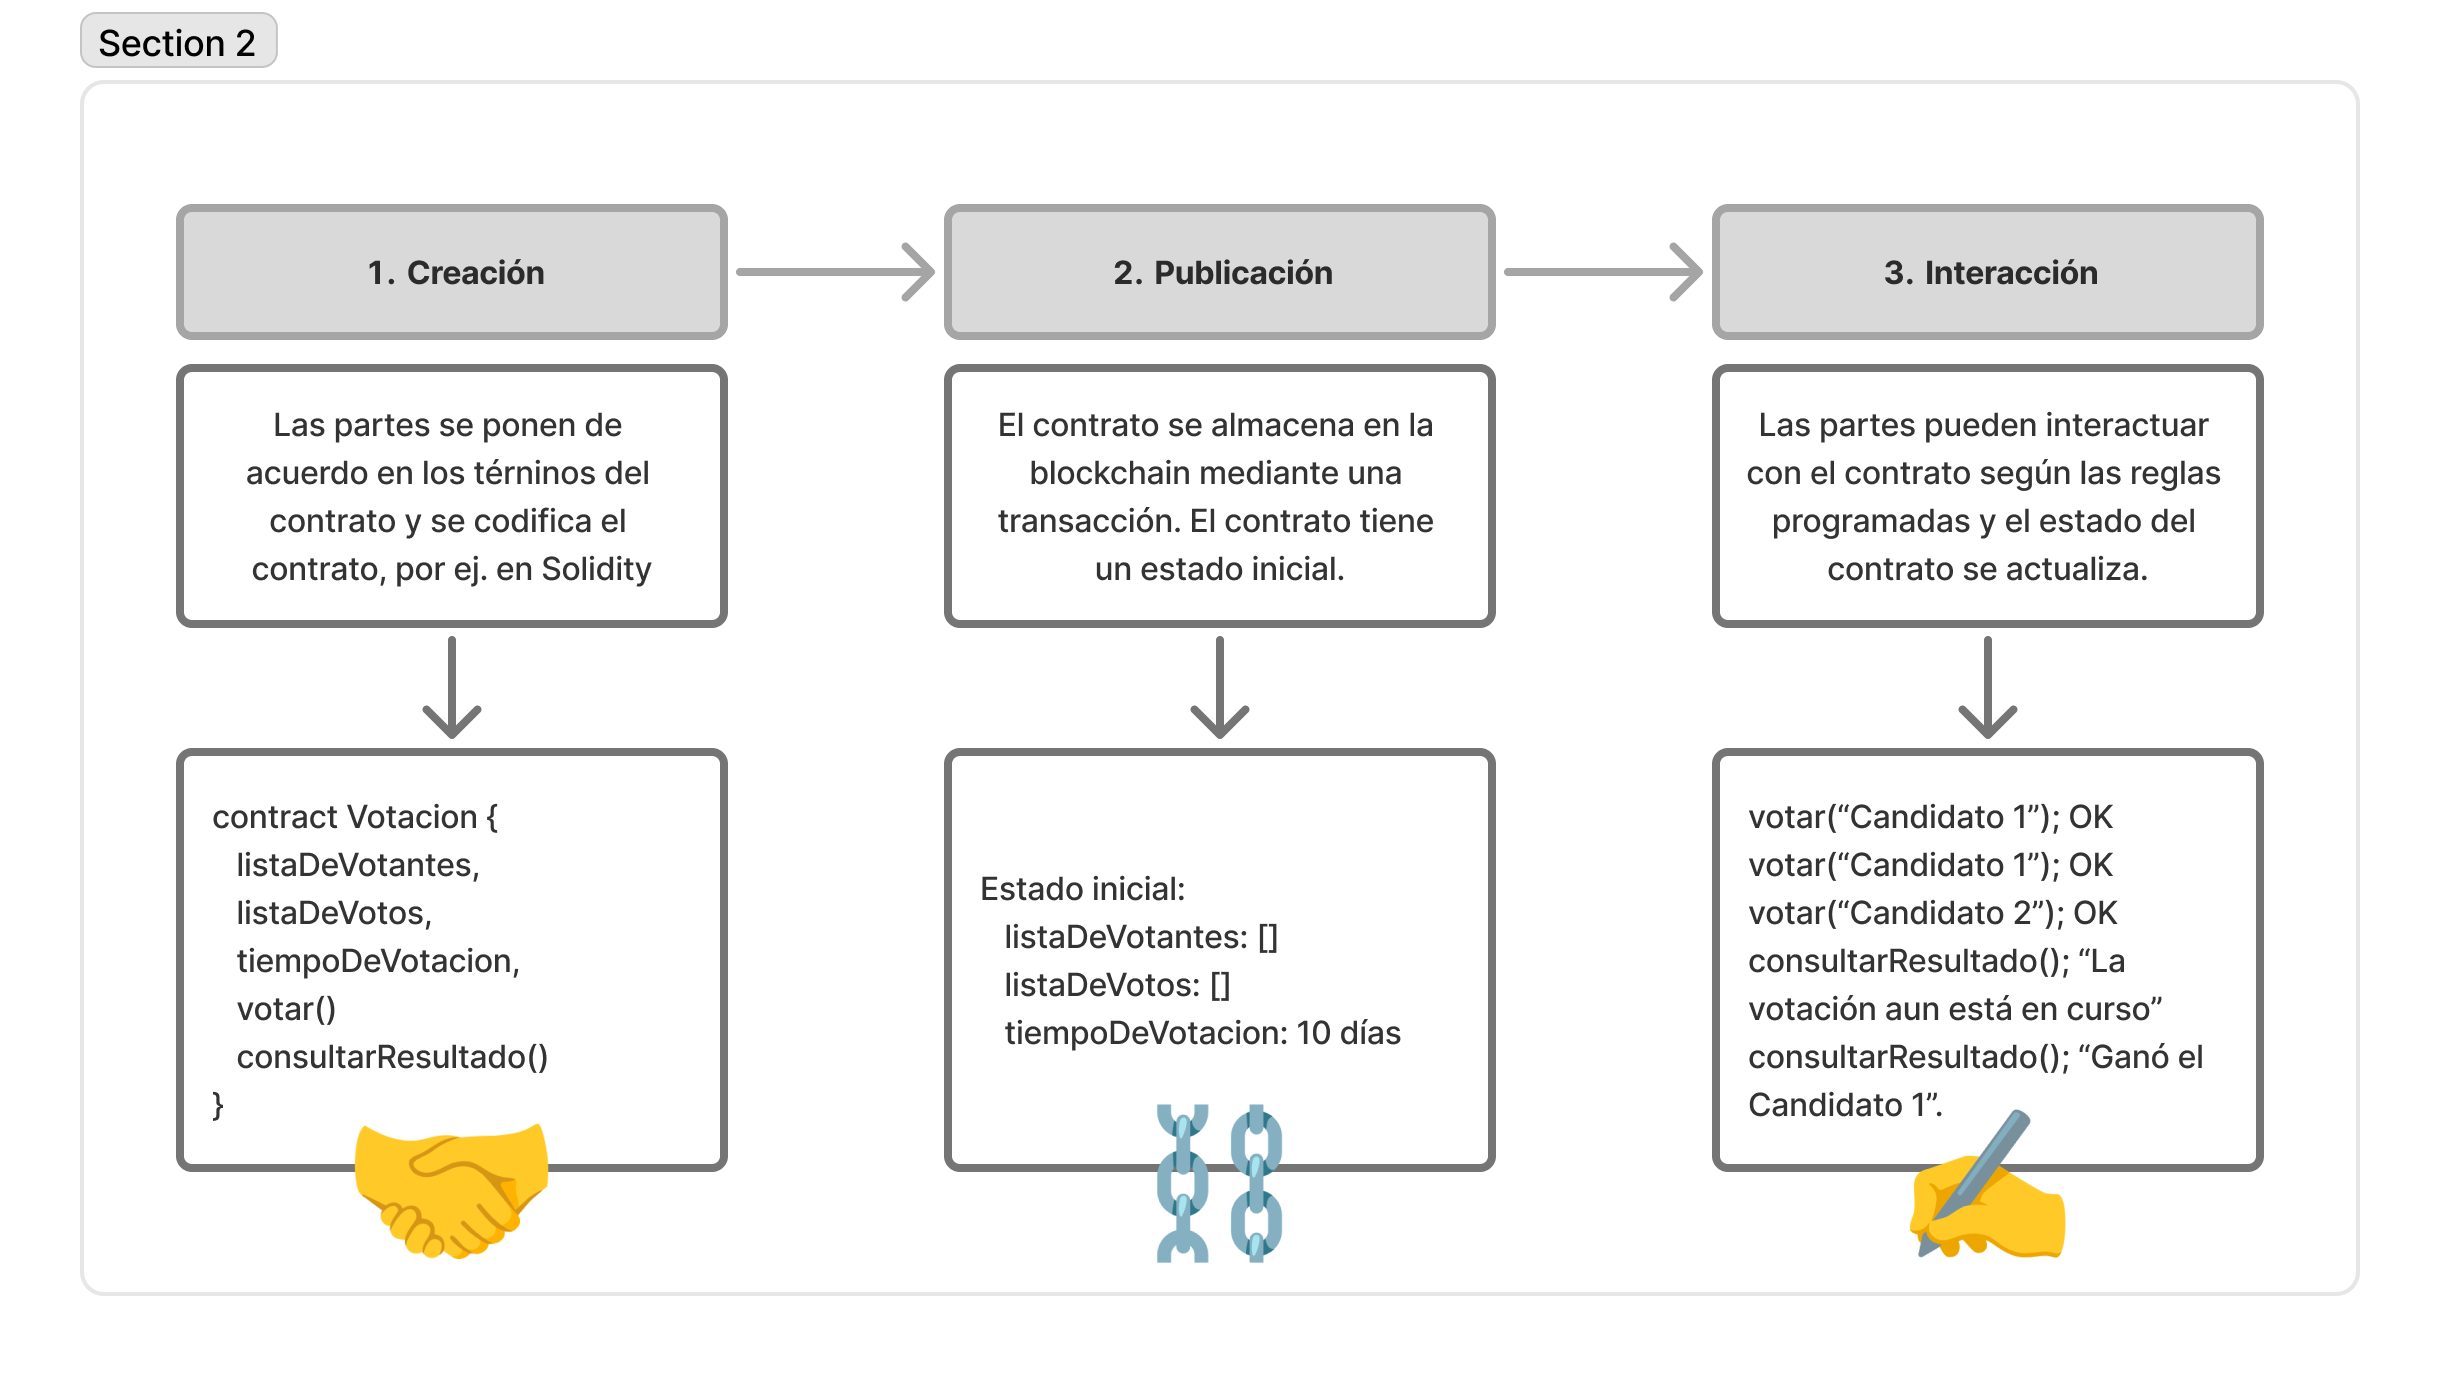
\includegraphics[width=0.8\textwidth]{Figures/smart-contract-process-voting.png}
    \caption{Proceso de creación y ejecución de un contrato inteligente}
    \label{fig:smart-contract-process}
\end{figure}

Además de las ventajas generales de la tecnología blockchain, los contratos inteligentes aportan beneficios y desafíos específicos frente a la automatización de procesos basada en sistemas digitales tradicionales. Entre sus principales ventajas, destacan la capacidad de ejecutar acuerdos de forma automática y verificable sin necesidad de intermediarios, la transparencia y auditabilidad del código y de su historial de transacciones, así como la posibilidad de integrarse con otros contratos para crear procesos más complejos. Estas propiedades permiten reducir fricciones operativas, agilizar procesos y ofrecer garantías criptográficas de que las reglas se cumplen tal como fueron definidas.

Sin embargo, los contratos inteligentes enfrentan limitaciones inherentes a las infraestructuras blockchain, principalmente en términos de escalabilidad \cite{kalajdjieski2023databases}. A diferencia de los sistemas centralizados que permiten ejecución paralela y optimización con bases de datos indexadas, los smart contracts operan bajo modelos de ejecución secuencial y replicación completa en cada nodo \cite{taherdoost2023smart}. Esto impacta directamente su rendimiento y complejiza la implementación de algoritmos avanzados. Desde la perspectiva de la ingeniería de software, el desarrollo de contratos inteligentes introduce restricciones no triviales: el código inmutable, los costos asociados al almacenamiento en cadena, la ausencia de llamadas externas directas y los modelos de estado global distribuido. Estas particularidades exigen la adopción de nuevas metodologías y prácticas de diseño seguro, control de flujos y validación estática, muchas de las cuales aún se encuentran en proceso de estandarización \cite{taherdoost2023smart, cepal2021economia}.

En síntesis, los contratos inteligentes constituyen una herramienta computacional que expande las fronteras de la programación distribuida y descentralizada. Si bien su potencial transformador es innegable \cite{taherdoost2023smart}, su desarrollo robusto y seguro representa un desafío activo que abarca múltiples dominios de la computación: desde la teoría de lenguajes formales \cite{hoskinson2017we} y la arquitectura de sistemas distribuidos, hasta la verificación de software, la criptografía aplicada y la integración de datos externos confiables \cite{taherdoost2023smart}. Debido a la aparición los contratos inteligentes, la tecnología blockchain ha trascendido su origen ligado a las criptomonedas para convertirse en un paradigma disruptivo con aplicaciones transversales en múltiples dominios \cite{bartolomeo2020introduccion, vaigandla2023review}. En la actualidad, los contratos inteligentes se posicionan como un componente fundamental y un impulsor clave de gran parte de las nuevas y complejas soluciones basadas en blockchain, especialmente aquellas que buscan automatizar procesos y gestionar la lógica de negocio directamente en la cadena \cite{sharabati2024blockchain}. Si bien representan una tecnología prometedora, aún se encuentran en una etapa incipiente, lo que implica la existencia de numerosos aspectos por perfeccionar \cite{taherdoost2023smart}. En un contexto más amplio, la tecnología blockchain, incluyendo a los contratos inteligentes, ofrece una serie de ventajas fundamentales y limitaciones inherentes que la distinguen de los sistemas de almacenamiento de datos tradicionales.

\subsection{Desafíos y Oportunidades}

Las características inherentes de la blockchain, detalladas previamente, se traducen en una serie de ventajas que la distinguen de tecnologías tradicionales. La descentralización propia de su diseño y la consecuente eliminación de intermediarios resultan en una mayor confianza \cite{rejeb2023role} y eficiencia operativa al prescindir de autoridades centrales \cite{sharabati2024blockchain}. La arquitectura basada en registros inmutables garantiza transparencia y trazabilidad completa \cite{sharabati2024blockchain}, permitiendo un historial verificable de cualquier activo o evento, lo cual es crucial para casos de uso como certificación \cite{bartolomeo2020introduccion}, logística \cite{bartolomeo2020introduccion, rejeb2023role} y gestión de residuos \cite{bulkowska2023implementation}. La inmutabilidad de los datos, reforzada por la seguridad criptográfica, asegura la integridad de la información \cite{sunny2022systematic} y una resistencia robusta a manipulaciones maliciosas y puntos únicos de falla \cite{bartolomeo2020introduccion}. Además, la capacidad de automatización de aplicaciones mediante contratos inteligentes optimiza la eficiencia y confiabilidad operativa al ejecutar condiciones lógicas de forma autónoma \cite{bartolomeo2020introduccion}. En conjunto, estas propiedades confieren a blockchain una aplicabilidad transversal que la consolida como una tecnología habilitadora para la transformación digital en sectores diversos como finanzas, salud, IoT, energía, educación y ciudades inteligentes.

Sin embargo, a pesar de sus beneficios, la tecnología blockchain también enfrenta desafíos y limitaciones significativos. Uno de los principales desafíos es la escalabilidad y el rendimiento \cite{tripathi2023comprehensive}. Las blockchains actuales suelen presentar un bajo \textit{throughput} en comparación con los sistemas centralizados \cite{baralla2023waste}, lo cual restringe su aplicación en escenarios de alta frecuencia transaccional. Esto se debe inherentemente a la necesidad de alcanzar un consenso distribuido y a la replicación completa de datos en todos los nodos \cite{tripathi2023comprehensive}. Otro reto importante es la interoperabilidad limitada, que dificulta la integración fluida entre distintas plataformas blockchain con infraestructuras externas preexistentes \cite{tripathi2023comprehensive}. En entornos públicos, la privacidad es una preocupación, ya que, aunque los usuarios pueden operar de manera seudónima, la visibilidad total de las transacciones en la cadena puede comprometer datos sensibles \cite{diez2023web, rennock2018blockchain}. Además, existen vulnerabilidades técnicas inherentes, como el ataque del 51\%, el doble gasto, los ataques Sybil, y la posibilidad de errores en contratos inteligentes mal programados, que requieren atención constante \cite{diez2023web}. La irreversibilidad de las transacciones, si bien es una garantía de seguridad, puede ser problemática ante vulnerabilidades de programación, errores o fraudes, ya que las operaciones registradas no pueden deshacerse \cite{taherdoost2023smart}. Por último, las limitaciones de almacenamiento representan un desafío práctico, dado que los nodos deben almacenar volúmenes crecientes de información, lo cual no escala eficientemente en redes de gran tamaño \cite{taherdoost2023smart}.

Estos desafíos, aunque significativos, están siendo abordados activamente por la investigación y el desarrollo en la comunidad blockchain. La constante evolución de la tecnología y la aparición de nuevas soluciones buscan mitigar estas limitaciones, abriendo el camino para una adopción más amplia \cite{tripathi2023comprehensive, baralla2023waste, taherdoost2023smart}. En este contexto de evolución y superación de barreras, la tecnología blockchain ha demostrado su potencial para transformar diversos sectores y abarcar numerosos casos de uso.

% \subsection{Casos de Uso}

En el sector financiero, blockchain ha generado disrupción mediante soluciones para pagos directos (con las llamadas criptomonedas), emisión de bonos, transferencias internacionales y operaciones en mercados de capital \cite{bartolomeo2020introduccion}. Instituciones como Santander y la Bolsa de Comercio de Santiago han adoptado esta tecnología para simplificar transacciones, automatizar registros y eliminar intermediarios \cite{bartolomeo2020introduccion}. Gracias a su estructura descentralizada y sus mecanismos criptográficos, blockchain permite mejorar la trazabilidad de los activos financieros. Pero si bien su uso en finanzas ha sido el más destacado desde sus comienzos con Bitcoin, la tecnología blockchain ha demostrado ser versátil y aplicable a una amplia gama de sectores, cada uno con sus propias necesidades y desafíos. Un conjunto de variados casos de uso evidencia cómo blockchain puede transformar modelos tradicionales mediante estructuras distribuidas, reglas codificadas y registros inmutables. Su implementación efectiva puede contribuir a una mayor eficiencia, confianza y sostenibilidad en distintas áreas del desarrollo económico, social y tecnológico.

A nivel gubernamental, blockchain ofrece nuevas herramientas para la modernización del Estado. Permite la gestión segura y verificable de identidades digitales, la trazabilidad de procesos administrativos, y la implementación de sistemas de votación transparentes \cite{vaigandla2023review}. Iniciativas como la European Blockchain Partnership buscan establecer una infraestructura digital pública para servicios intergubernamentales \cite{diez2023web}. En el ámbito de la salud, blockchain permite almacenar registros médicos de manera segura y distribuida, mejorando la interoperabilidad entre instituciones y permitiendo a los pacientes un mayor control de su historial médico \cite{sunny2022systematic}. Esta tecnología también se utiliza en la trazabilidad de la cadena de suministro farmacéutica y en la supervisión de ensayos clínicos, donde se requiere un alto nivel de confianza y se debe garantizar cumplimiento normativo \cite{vaigandla2023review}. En otros rubros, como la educación, esta tecnología se utiliza para la emisión y verificación de certificados académicos inmutables y descentralizados. Universidades como Nicosia o la de Murcia ya utilizan blockchain para certificar diplomas y logros académicos \cite{diez2023web}. En IoT, facilita la recolección y gestión segura de datos en tiempo real \cite{sunny2022systematic}. En contabilidad y auditoría, posibilita libros contables distribuidos con transparencia total y reducción de fraudes \cite{bartolomeo2020introduccion}. A su vez, también se está utilizando blockchain para crear mercados para el comercio de energía entre pares, mejorando la gestión de certificados de energías renovables y optimizando la trazabilidad de producción y consumo energético \cite{sunny2022systematic, vaigandla2023review}.

En el ámbito de la gestión de la cadena de suministro (SCM), blockchain proporciona una plataforma confiable para garantizar la trazabilidad, autenticidad y visibilidad en tiempo real de productos y materiales \cite{torres2022tendencias, sharabati2024blockchain}. Empresas como IBM, Maersk y FedEx han implementado soluciones blockchain para monitorear inventarios, registrar pagos y reducir disputas logísticas \cite{tripathi2023comprehensive}. Casos como el de Dervinsa en Argentina, que certifica la calidad de productos derivados de residuos de vinificación, y otras iniciativas que aplican trazabilidad a alimentos y textiles, muestran cómo esta tecnología fortalece el control de calidad y la confianza en los mercados \cite{bartolomeo2020introduccion}. Además, en contextos más amplios, blockchain permite una sincronización eficiente entre departamentos, la reducción de riesgos de falsificación y la mejora general de la sostenibilidad operativa \cite{sunny2022systematic}.

Dentro de modelos de economía circular, blockchain se posiciona como un facilitador para monitorear ciclos de vida de productos y materiales, ofreciendo transparencia y responsabilidad en la gestión de residuos \cite{bulkowska2023implementation, baralla2023waste}. Diversos tipos de residuos, desde plásticos y vidrio hasta electrónicos y biomédicos, pueden ser gestionados de manera más eficiente mediante el uso de contratos inteligentes que automatizan verificaciones, recompensas e interacciones entre actores de la cadena \cite{baralla2023waste}. Asimismo, han surgido propuestas innovadoras como la generación de pasaportes digitales de productos y esquemas de incentivos sostenibles, promoviendo hábitos de consumo responsables y nuevos modelos de negocio circulares \cite{baralla2023waste}.

La necesidad de trazar el flujo de materiales, certificar la autenticidad de los procesos productivos y garantizar la gestión responsable de residuos, ha posicionado a blockchain como una herramienta protagónica para habilitar modelos circulares sostenibles. En particular, su capacidad para registrar datos inmutables y automatizar interacciones mediante contratos inteligentes permite estructurar sistemas de trazabilidad que no sólo mejoran la eficiencia, sino que también fortalecen la confianza entre actores y fomentan la rendición de cuentas \cite{sharabati2024blockchain, rejeb2023role}. A continuación, se analizará con mayor profundidad el uso de blockchain para trazabilidad de materiales en la cadena de suministros y para la implementación de estrategias de economía circular.

\section{Economía Circular}
\label{sec:circular-economy}

La economía circular es un enfoque alternativo al modelo económico lineal tradicional, que nace con el objetivo transformar de manera sostenible la forma en que la sociedad produce, consume y gestiona los recursos naturales.

Desde la Revolución Industrial, la economía global ha operado principalmente bajo un modelo lineal de ``extraer, producir y consumir``, caracterizado por la explotación de recursos naturales y la generación masiva de residuos \cite{cerda2016economia}. En este modelo económico, los recursos son extraídos de la naturaleza, transformados en productos, consumidos y finalmente desechados al terminar su vida útil. Este enfoque, aunque ha impulsado un crecimiento económico mundial sin precedentes, ha generado sobreexplotación y degradación de ecosistemas. La deforestación, pérdida de biodiversidad, contaminación del agua, generación masiva de residuos y escasez de recursos no renovables son algunas de las consecuencias negativas de este enfoque extractivo a gran escala. A medida que la población mundial y la demanda de recursos continúan creciendo, la insostenibilidad de este modelo a largo plazo se hace cada vez más evidente \cite{clima2022book}.

En contraste con la economía lineal, la economía circular propone un sistema en el que los recursos se mantienen en uso durante el mayor tiempo posible, se reciclan y se reutilizan, minimizando la generación de residuos y reduciendo la extracción de materias primas \cite{ellenmacarthurfoundation2022}. La economía circular propone un cambio radical de paradigma, al concebir los sistemas productivos y de consumo como ciclos cerrados. Este enfoque se basa en los principios de diseño ecológico, la reutilización de materiales y la regeneración de los sistemas naturales, con el objetivo de crear un sistema económico más sostenible y resiliente. La diferencia estructural entre la economía lineal y la economía circular se hace evidente al ilustrar el flujo de recursos en ambos modelos, como se muestra en la Figura \ref{fig:circular-linear-economy-comparison}.

\begin{figure}[!tb]
    \centering
    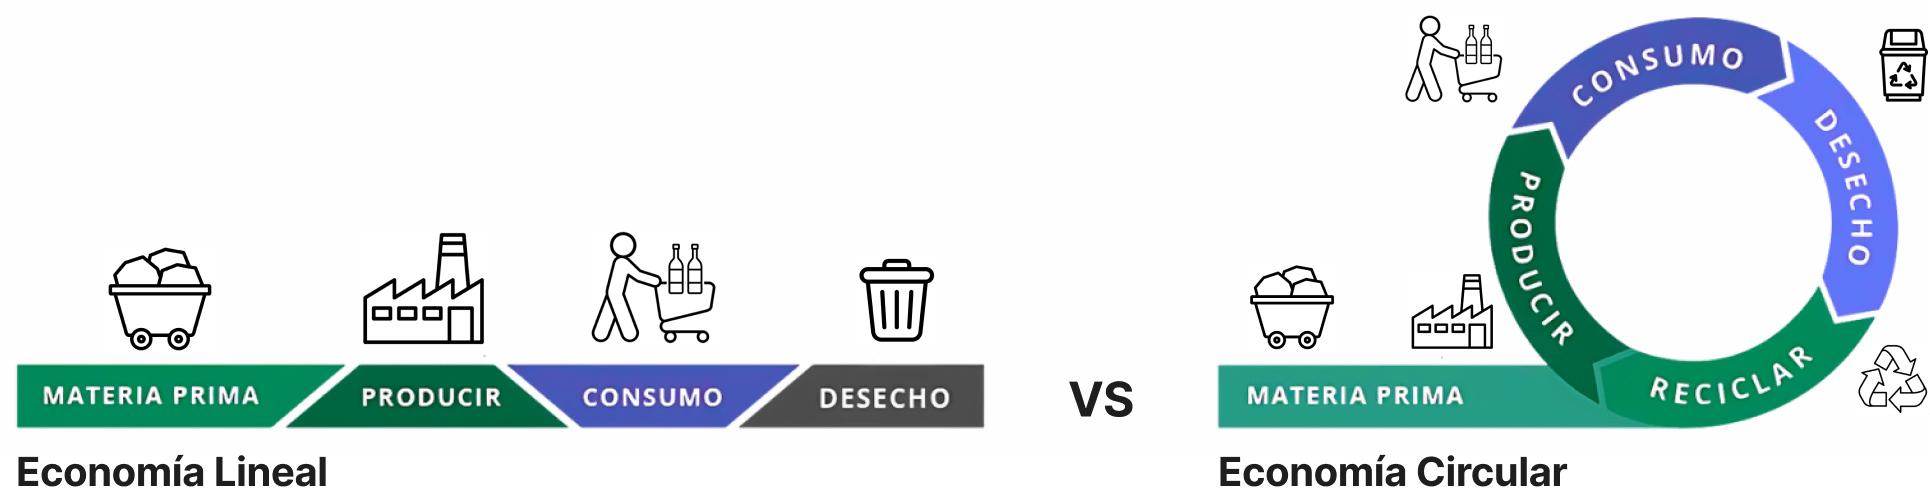
\includegraphics[width=0.8\textwidth]{Figures/circular-linear-economy-comparison.png}
    \caption{Comparación entre la economía lineal y la economía circular}
    \label{fig:circular-linear-economy-comparison}
\end{figure}

En el enfoque lineal, la cadena de suministro de materiales se organiza como un proceso unidireccional: los recursos son extraídos, transformados en productos, consumidos y finalmente desechados. Este modelo ignora el valor residual de los materiales, no contempla mecanismos para reincorporar los productos al ciclo productivo una vez finalizada su vida útil y, en consecuencia, genera una creciente acumulación de residuos. En contraste, la economía circular redefine el papel de la cadena de suministros, transformándola en una red cerrada y regenerativa. Con este enfoque, la cadena se vuelve más dinámica e interdependiente, integrando bucles de retroalimentación entre los diferentes actores de la cadena de valor, incluyendo a consumidores, productores, proveedores y gestores de residuos. 

A nivel sistémico, la economía circular se concibe como una evolución hacia un sistema más integrado, resiliente y sostenible. Su implementación es paulatina, en forma de transición desde el modelo lineal predominante hacia un modelo circular. Esta transición requiere una transformación estructural en los sistemas productivos en múltiples niveles: diseño de productos, procesos logísticos, distribución y gestión del fin de vida útil. Entre los habilitadores clave de este proceso de transición, se encuentra la trazabilidad, entendida como la capacidad de rastrear el origen, el uso y el destino de materiales y productos a lo largo de toda su vida útil. La trazabilidad permite verificar compromisos ambientales, controlar impactos, optimizar la logística inversa y empoderar tanto a consumidores como a instituciones para adoptar decisiones basadas en información confiable.

En la actualidad existen desafíos culturales, normativos y tecnológicos que dificultan la implementación de la economía circular a gran escala. La transición de los sistemas productivos requiere inversión en infraestructura, marcos regulatorios adecuados y políticas de incentivos claros. Asimismo, implica repensar la educación y la formación de trabajadores para adaptarse a nuevas dinámicas laborales. En muchos contextos, como América Latina y el Caribe, también se han identificado limitaciones institucionales y de gobierno que deben ser abordadas para permitir una adopción efectiva del modelo.

Es importante destacar que esta transición ya se encuentra en marcha. Numerosos países, regiones y sectores productivos han comenzado a incorporar principios circulares en sus estrategias de desarrollo, en muchos casos impulsados por marcos regulatorios, acuerdos internacionales y metas vinculadas a la sostenibilidad ambiental. En este contexto, las políticas públicas han asumido un rol central como motores de adopción, ofreciendo instrumentos normativos, fiscales y de gobernanza que facilitan la transformación del sistema económico. %A continuación, se analizarán algunas políticas sustentables relevantes para avanzar hacia una economía más circular y resiliente.

\subsection{Políticas sustentables}

En el proceso de transición hacia modelos de desarrollo más sostenibles, la Unión Europea ha asumido un rol pionero en la implementación de políticas públicas alineadas con la economía circular. Iniciativas como el Pacto Verde Europeo y la Ley Europea del Clima han consolidado a Europa como un referente global en materia de sustentabilidad ambiental. Estas políticas no solo promueven la descarbonización de la economía, sino que también introducen principios de circularidad en sectores como la industria, la energía, la movilidad y la gestión de residuos, reconfigurando las cadenas de suministro hacia sistemas más regenerativos, transparentes y trazables.

Sin embargo, el mayor hito internacional en la construcción de una visión compartida sobre sustentabilidad ha sido la adopción de los Objetivos de Desarrollo Sostenible (ODS) de Naciones Unidas en 2015. Este conjunto de 17 objetivos interconectados, acompañados por 169 metas y más de 230 indicadores, propone una agenda universal que orienta las políticas públicas hacia un desarrollo económico, social y ambiental equilibrado para 2030.

\begin{figure}[!tb]
    \centering
    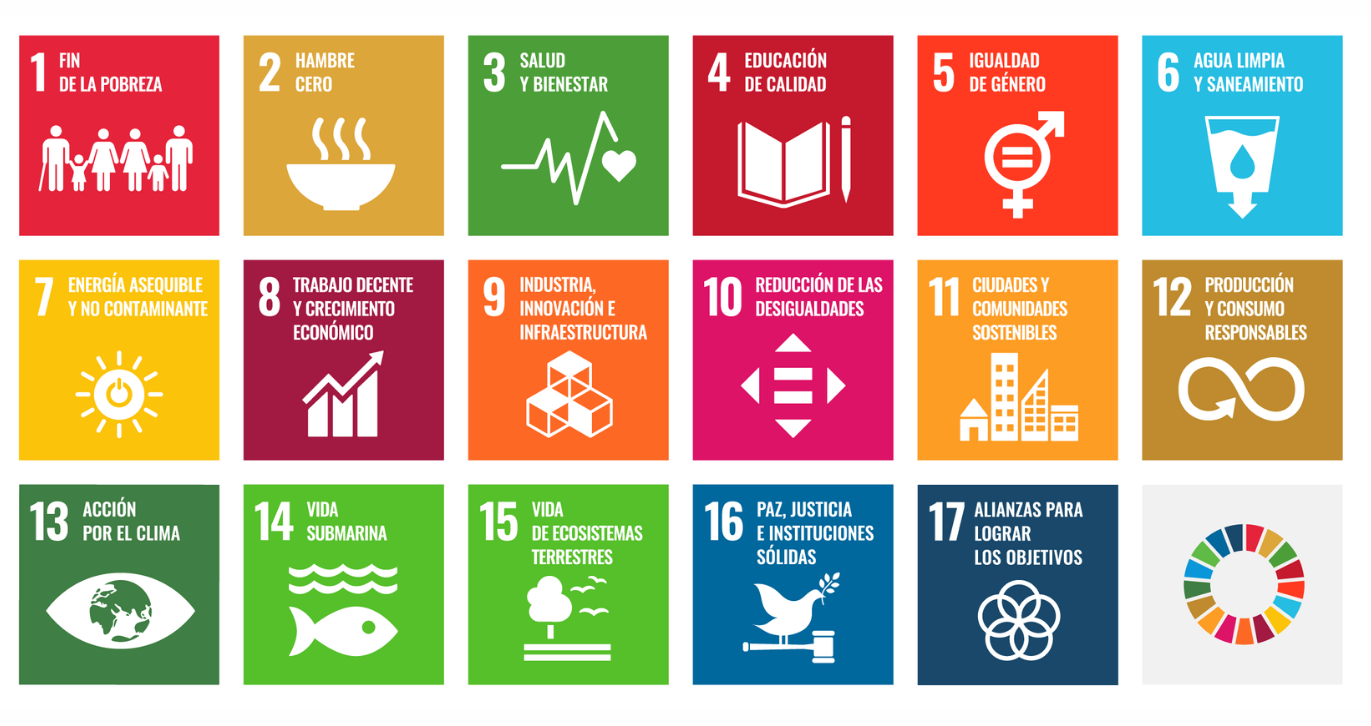
\includegraphics[width=0.8\textwidth]{Figures/ods.png}
    \caption{Objetivos de Desarrollo Sostenible (ODS) de Naciones Unidas}
    \label{fig:ods}
\end{figure}

El objetivo general de los ODS es erradicar la pobreza, proteger el planeta y garantizar la paz y prosperidad para todas las personas. En relación con la economía circular, se identifican un conjunto de objetivos particularmente relevantes que guían tanto los marcos normativos como las estrategias de innovación en producción, consumo y gestión de residuos:

\begin{itemize}
\item \textbf{ODS 7: Energía asequible y no contaminante.}\footnote{\url{https://www.un.org/sustainabledevelopment/es/energy/}} Promueve el acceso universal a fuentes de energía limpias, eficientes y modernas, fundamentales para la transición a una economía circular descarbonizada.
\item \textbf{ODS 11: Ciudades y comunidades sostenibles.}\footnote{\url{https://www.un.org/sustainabledevelopment/es/cities/}} Plantea la necesidad de gestionar de manera integrada los recursos urbanos, incluyendo residuos, infraestructura y movilidad, en articulación con una trazabilidad eficiente de los flujos materiales.
\item \textbf{ODS 12: Producción y consumo responsables.}\footnote{\url{https://www.un.org/sustainabledevelopment/es/sustainable-consumption-production/}} Es el núcleo del paradigma circular, impulsando el diseño sostenible de productos, el uso eficiente de recursos, la minimización de residuos y la promoción de modelos de cadena de suministro regenerativos.
\item \textbf{ODS 13: Acción por el clima.}\footnote{\url{https://www.un.org/sustainabledevelopment/es/climate-change-2/}} Vincula la circularidad con la reducción de emisiones y la adaptación al cambio climático, incentivando políticas que rediseñen los sistemas productivos de alto impacto ambiental.
\end{itemize}

Los ODS han generado un marco de referencia común que ha influido fuertemente en las agendas de sostenibilidad a nivel global, incluyendo América Latina. Aunque en la región la adopción de políticas circulares aún es incipiente en comparación con Europa, se observan avances significativos en la última década. Por ejemplo, varios países han comenzado a incorporar la responsabilidad extendida del productor, prohibiciones de plásticos de un solo uso y normativas orientadas a la reutilización y reciclado de materiales. Estas políticas buscan reestructurar las cadenas de valor y fomentar prácticas productivas y logísticas compatibles con los principios de circularidad.

En Argentina, la Estrategia Nacional de Consumo y Producción Sostenibles se destaca como el instrumento central para avanzar hacia la economía circular. La estrategia integra medidas normativas, educativas, tecnológicas y financieras, orientadas a fortalecer la sostenibilidad en toda la cadena de producción y consumo. Promueve activamente el uso de tecnologías limpias, la gestión sostenible de recursos, y la incorporación de criterios ambientales en compras públicas, reconociendo el rol central de la trazabilidad como mecanismo para garantizar la transparencia, eficiencia y cumplimiento normativo en los sistemas productivos y sus cadenas de suministro.

% Si bien estos esfuerzos representan un paso importante, los desafíos estructurales persisten. La región enfrenta obstáculos en términos de infraestructura, financiamiento, coordinación institucional y disponibilidad de información confiable. A pesar de ello, el impulso dado por los ODS ha generado una convergencia regional que permite imaginar una transición hacia modelos circulares, sostenida por políticas públicas que consideran no sólo las metas globales, sino también las realidades locales.

Estas políticas dejan ver que la transformación hacia una economía circular no puede pensarse sin una reconfiguración de las cadenas de suministro, que constituyen la columna vertebral de los sistemas productivos. La implementación de políticas sustentables, tanto en Europa como en América Latina, ha puesto en evidencia la necesidad de contar con mecanismos que permitan monitorear, verificar y optimizar el flujo de materiales a lo largo de todo el ciclo de vida de los productos. En la siguiente sección se abordará con mayor detalle cómo se articula esta relación entre cadenas de suministro y trazabilidad, y cuál es su rol estratégico en la transición hacia un modelo económico circular.

\subsection{Cadena de suministro}
\label{sec:supply-chain}

En el contexto de la economía circular, la cadena de suministro asume una nueva lógica de funcionamiento. Pasa de ser una secuencia finita de pasos que culminan con el consumo y disposición del producto, a transformarse en un sistema cíclico, en el cual los productos son diseñados para permanecer en uso el mayor tiempo posible y ser reutilizados, reacondicionados o reciclados. 

La cadena de suministro constituye el entramado logístico, operativo y estratégico que permite el flujo de materiales, información y recursos desde la extracción de materias primas hasta la llegada de un producto al consumidor final. Este sistema complejo involucra a múltiples actores: proveedores, fabricantes, distribuidores, comerciantes, consumidores y, en el caso del modelo circular, gestores de residuos y autoridades regulatorias. Su objetivo es garantizar que los bienes y servicios se produzcan y entreguen de manera eficiente, segura y rentable. 

\begin{figure}[!tb]
    \centering
    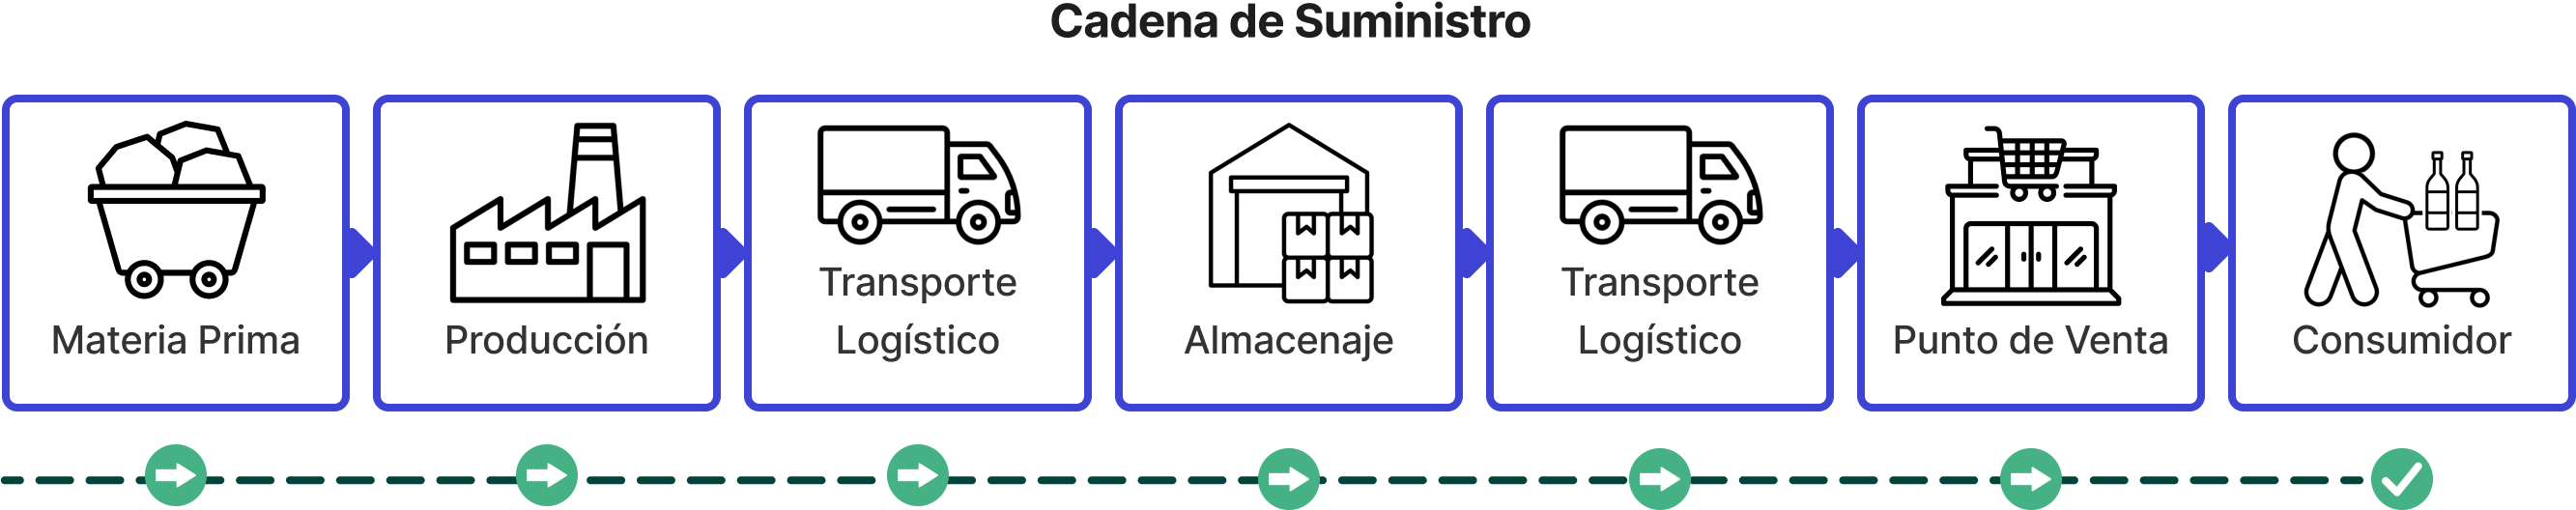
\includegraphics[width=0.8\textwidth]{Figures/supply-chain.png}
    \caption{Componentes de una cadena de suministro}
    \label{fig:supply-chain}
\end{figure}

A lo largo de los años, las cadenas de suministro se han establecido para maximizar la eficiencia y reducir costos en la producción de productos. Con este objetivo claro, es que se ha dividido el proceso en etapas y se aplican herramientas, procesos y tecnologías diversas para optimizar cada una de ellas, desde la adquisición de materias primas hasta la distribución final. Sin embargo, la maximización de la eficiencia en este modelo lineal, sin preocuparse por el destino del producto luego de su uso, ha generado efectos secundarios adversos en el medioambiente que, como ya se mencionó, han llevado a la necesidad de un modelo sostenible en el tiempo.

Transicionar una cadena de suministros desde un modelo lineal hacia uno circular implica una inversión en rediseño de productos, procesos y creación de nuevas relaciones y colaboraciones entre los actores involucrados. En muchos casos los distintos actores de la cadena lo perciben como una inversión sin retorno inmediato o como un costo adicional, lo que dificulta su adopción. Sin embargo, las políticas sostenibles y regulaciones previamente mencionadas, entre otras, están impulsando a las empresas a adoptar prácticas circulares, no solo por responsabilidad social, sino también por la presión del mercado y de las autoridades reguladoras.

Para diseñar una cadena de suministros circular, la trazabilidad se posiciona como la herramienta que permite mantener y mejorar la eficiencia y costos, mientras que permite incorporar al final de la cadena las etapas de disposición, reciclaje y reutilización de materiales. Sin una trazabilidad robusta en cadenas donde intervienen múltiples organizaciones y tecnologías, es difícil garantizar que los materiales se manipulen de manera adecuada, se traten, se reciclen y efectivamente se reincorporen al ciclo productivo.

La trazabilidad es la capacidad de seguir el recorrido completo de un producto, material o componente a lo largo de toda la cadena de suministro, desde su origen hasta su destino final. Su objetivo principal es reconstruir el historial de producción, transformación y movimiento de un bien, permitiendo conocer su composición, ubicación, responsables y condiciones de manejo en cada etapa del proceso. Por ejemplo, aplicando trazabilidad en la producción de vino se puede conocer la parcela de origen de la uva, la fecha de la vendimia y el proceso de añejamiento, permitiendo al consumidor verificar su autenticidad y al productor identificar rápidamente cualquier problema en un lote. Otro ejemplo frecuente es la trazabilidad de residuos peligrosos, que permite verificar que la disposición final del residuo se hizo correctamente para evitar riesgos de salud o ambientales. La información permite verificar la autenticidad del producto, asegurar estándares de calidad, cumplimiento normativo, eficiencia operativa y sostenibilidad ambiental. Procesos de trazabilidad establecidos permiten también identificar riesgos y oportunidades de mejora en la cadena, permitiendo optimizar la logística, reducir costos y riesgos asociados a errores, fraudes o contaminaciones, y mejorar la capacidad de respuesta ante incidentes o fallas. En la cadena de suministro, la trazabilidad se aplica de forma transversal, es decir, atraviesa e interconecta todas las fases del ciclo: desde el diseño y la fabricación, hasta la distribución, el consumo, la gestión de residuos y el reciclaje.

\begin{figure}[!tb]
    \centering
    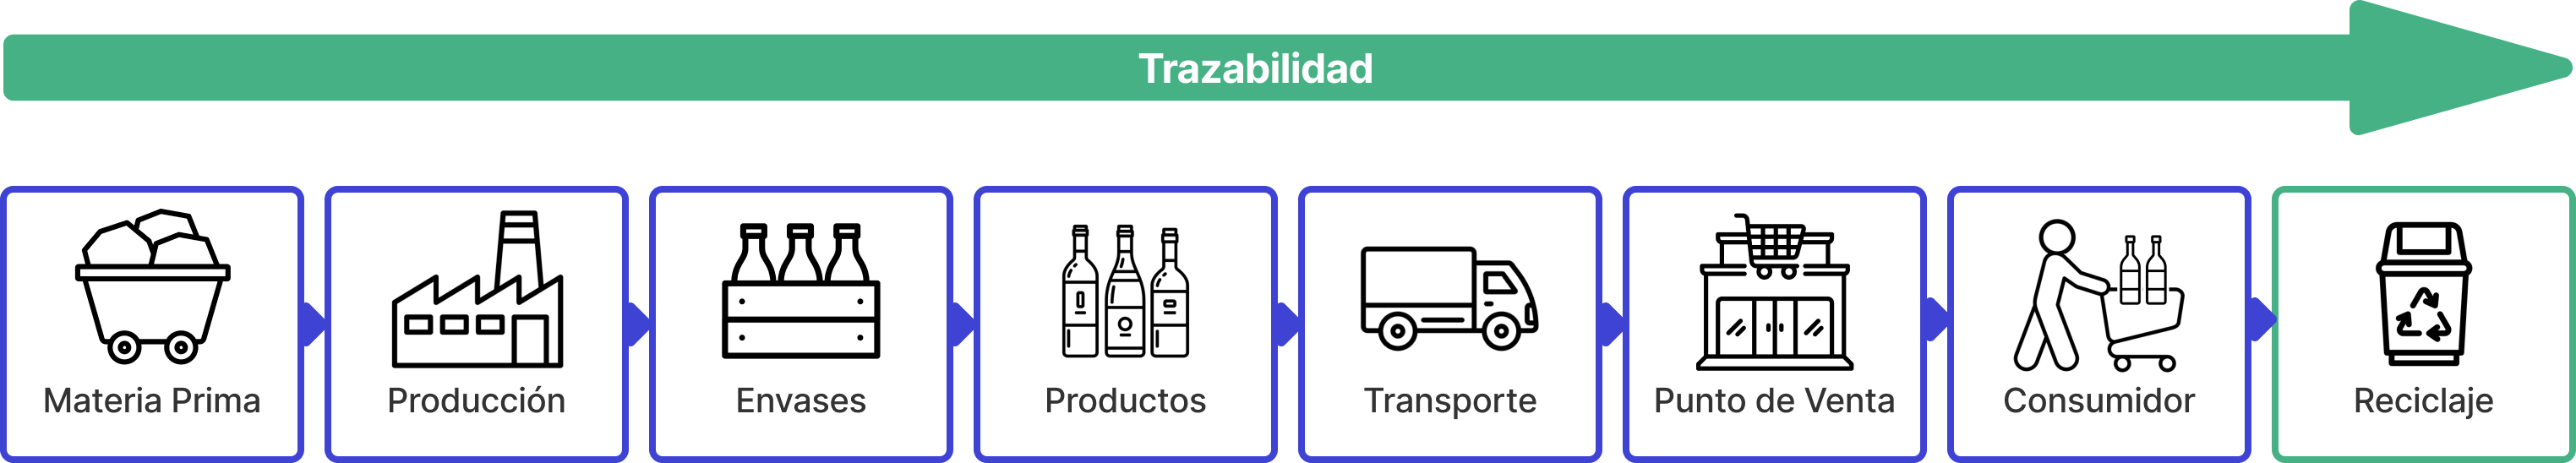
\includegraphics[width=0.8\textwidth]{Figures/supply-chain-traceability.png}
    \caption{Ejemplo de trazabilidad como herramienta transversal en la cadena de suministro de envases de vino}
    \label{fig:supply-chain-traceability}
\end{figure}

No obstante, la implementación de trazabilidad en la cadena de suministro conlleva desafíos importantes. Las cadenas de suministro tradicionales suelen estar fragmentadas y utilizar sistemas de información heterogéneos o poco interoperables. Muchos registros todavía se realizan en papel o en bases de datos centralizadas, lo que aumenta la vulnerabilidad frente a errores humanos, pérdidas de datos o manipulaciones. Además, la ausencia de estándares unificados y la reticencia a compartir datos entre organizaciones limitan la visibilidad total del flujo de productos y materiales. Para abordar estos desafíos, se ha desarrollado un conjunto de tecnologías que fortalecen los sistemas de trazabilidad. Entre las más utilizadas se encuentran los códigos de barras y las etiquetas RFID, que permiten la identificación automática de productos mediante etiquetas físicas; los sensores IoT, que capturan datos en tiempo real sobre condiciones ambientales o de transporte; los sistemas ERP y de gestión logística digitales, que centralizan y organizan la información operativa; y, más recientemente, la tecnología blockchain se está posicionando como solución para unificar a todos los actores de la cadena aportando una nueva capa de transparencia entre etapas y resolviendo problemas de confianza entre los diferentes actores.

La tecnología blockchain en la cadena de suministros permite registrar cada transacción o evento de la cadena en una base de datos digital descentralizado e inalterable. Esto garantiza que todos los actores tengan acceso a un historial común y verificable, reduciendo la necesidad de intermediarios y auditores externos. Combinando contratos inteligentes y plataformas de análisis de datos, la trazabilidad basada en blockchain permite no solo conocer lo que ocurrió, sino también automatizar respuestas ante condiciones predefinidas, reduciendo los tiempos de reacción y aumentando la confianza entre las partes. El uso de blockchain en este contexto aporta un aumento significativo en la seguridad, transparencia, precisión de datos, eficiencia, responsabilidad y confianza entre actores. Esta tecnología ya se está utilizando para trazabilidad en diversos sectores como la agricultura, alimentos, industria textil y medioambiente. Por ejemplo, en el sector alimenticio, impulsa el valor percibido del producto y la calidad, además de fortalecer la confianza entre las partes interesadas. Para el sector industrial, se enfoca en la planeación y el intercambio de información para una mayor sostenibilidad. Además, es posible combinar tecnología Blockchain con IoT y otros sistemas digitales ya implementados en la cadena de suministros. Esta combinación puede proporcionar soluciones aún más eficientes para la cadena de suministro, automatizando la recopilación de datos confiables y aumentando los beneficios para las partes interesadas.

La trazabilidad basada en blockchain ya se está aplicando en la cadena de suministros de diversos sectores con el objetivo de transicionar a una economía circular. Su adopción aún está en desarrollo, pero su potencial para optimizar la trazabilidad y la sostenibilidad en la gestión de residuos es ampliamente reconocido. Aplicar trazabilidad para la economía circular permite unir la producción con el reciclaje, posibilitando no solo verificar el cumplimiento de estándares ambientales y sociales en gestión de residuos, sino también optimizar el uso de recursos, reducir desperdicios y fomentar la reutilización y el uso de materiales reciclados de calidad en nuevos productos. A continuación, se explorará cómo se articula el proceso de producción y reciclaje en la economía circular, y cómo la trazabilidad digital puede potenciar este ciclo.

\subsection{Proceso de producción y reciclaje en la economía circular}

En el marco de la economía circular, los procesos de producción y reciclaje dejan de concebirse como etapas aisladas y unidireccionales para integrarse en un sistema dinámico y regenerativo. En este esquema, la cadena de suministros del proceso productivo incluye la gestión de residuos y la reinserción de materiales reciclados en nuevos ciclos productivos. 

\begin{figure}[!tb]
    \centering
    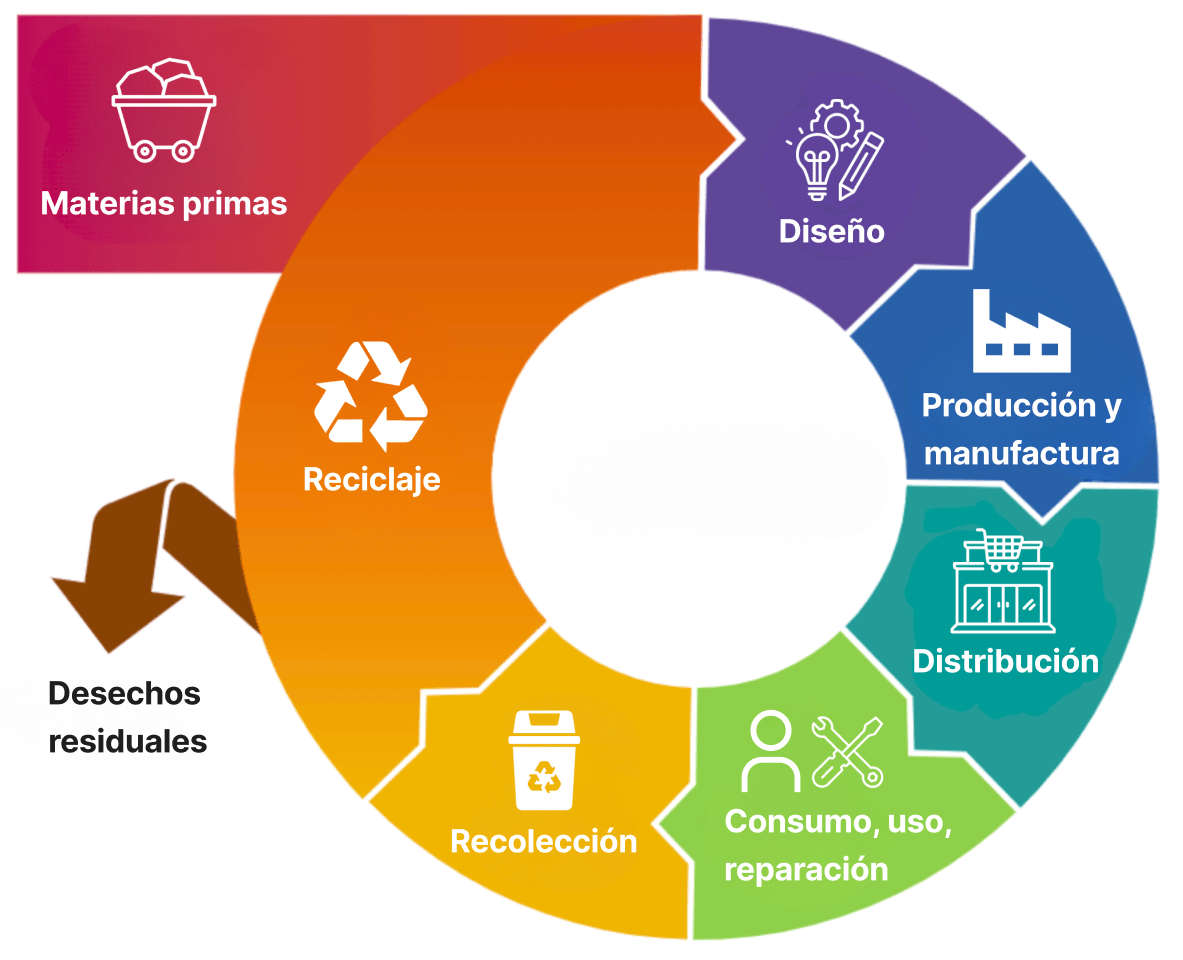
\includegraphics[width=0.6\textwidth]{Figures/circular-economy-stages.png}
    \caption{Ciclo productivo de la economía circular}
    \label{fig:circular-economy-stages}
\end{figure}

El proceso de producción comienza propiamente con la etapa de diseño, donde se decide la composición de los productos considerando criterios de ecoeficiencia, reutilización y reciclabilidad. Aquí intervienen diseñadores, ingenieros y proveedores de materias primas, quienes priorizan materiales reciclados o de bajo impacto ambiental. A continuación, durante la fabricación, los procesos industriales buscan reducir el uso de recursos y minimizar las emisiones, integrando tecnologías limpias y eficientes. En esta fase, los productos terminados o semielaborados quedan registrados con información detallada sobre su origen, composición y trazabilidad, lo cual permite una futura gestión más eficiente de su reciclaje. Tras su elaboración, los productos son distribuidos a través de canales logísticos que buscan optimizar los costos e impacto ambiental del transporte y almacenamiento.

Una vez que los productos son utilizados por los consumidores, comienza el ciclo inverso de valorización. Cuando estos artículos llegan al fin de su vida útil (y ya no pueden ser reutilizados), se convierten en residuos que deben ser recolectados, transportados, clasificados y reciclados o reacondicionados. Este proceso, conocido de forma genérica como ``reciclaje`` (sin distinguir si el destino final es reacondicionamiento o reciclaje), involucra a recolectores, centros de acopio, plantas de tratamiento, recicladores industriales y fabricantes secundarios. Durante la recolección, tecnologías como sensores IoT, lectores de códigos QR o etiquetas RFID permiten registrar información sobre la identidad del recolector, la cantidad, el tipo y las condiciones del residuo. Esta información permite monitorear flujos de materiales y brindar transparencia en la cadena. En el primer paso del proceso de reciclaje, los residuos son transportados a instalaciones donde se clasifican y segregan según su tipo y calidad. Este paso es fundamental para evitar contaminaciones cruzadas entre materiales distintos y asegurar un reciclaje efectivo. Posteriormente, los materiales seleccionados se someten a procesos de reciclaje o reacondicionamiento, reincorporándolos al sistema productivo como insumos o productos reutilizables. En todo este proceso, tecnologías como blockchain pueden documentar cada transacción o transformación del material, documentando la integridad del proceso y fomentando la confianza entre los actores.

El esquema de la Figura \ref{fig:baralla-model-1} ilustra las distintas aplicaciones posibles de la tecnología blockchain en cada etapa del ciclo completo de economía circular. En este sistema ilustrado, la tecnología blockchain conecta las etapas en un flujo de información unificada, formando un sistema de trazabilidad digital que permite el seguimiento de los materiales desde su origen hasta su reincorporación al sistema o disposición final.

\begin{figure}[!tb]
    \centering
    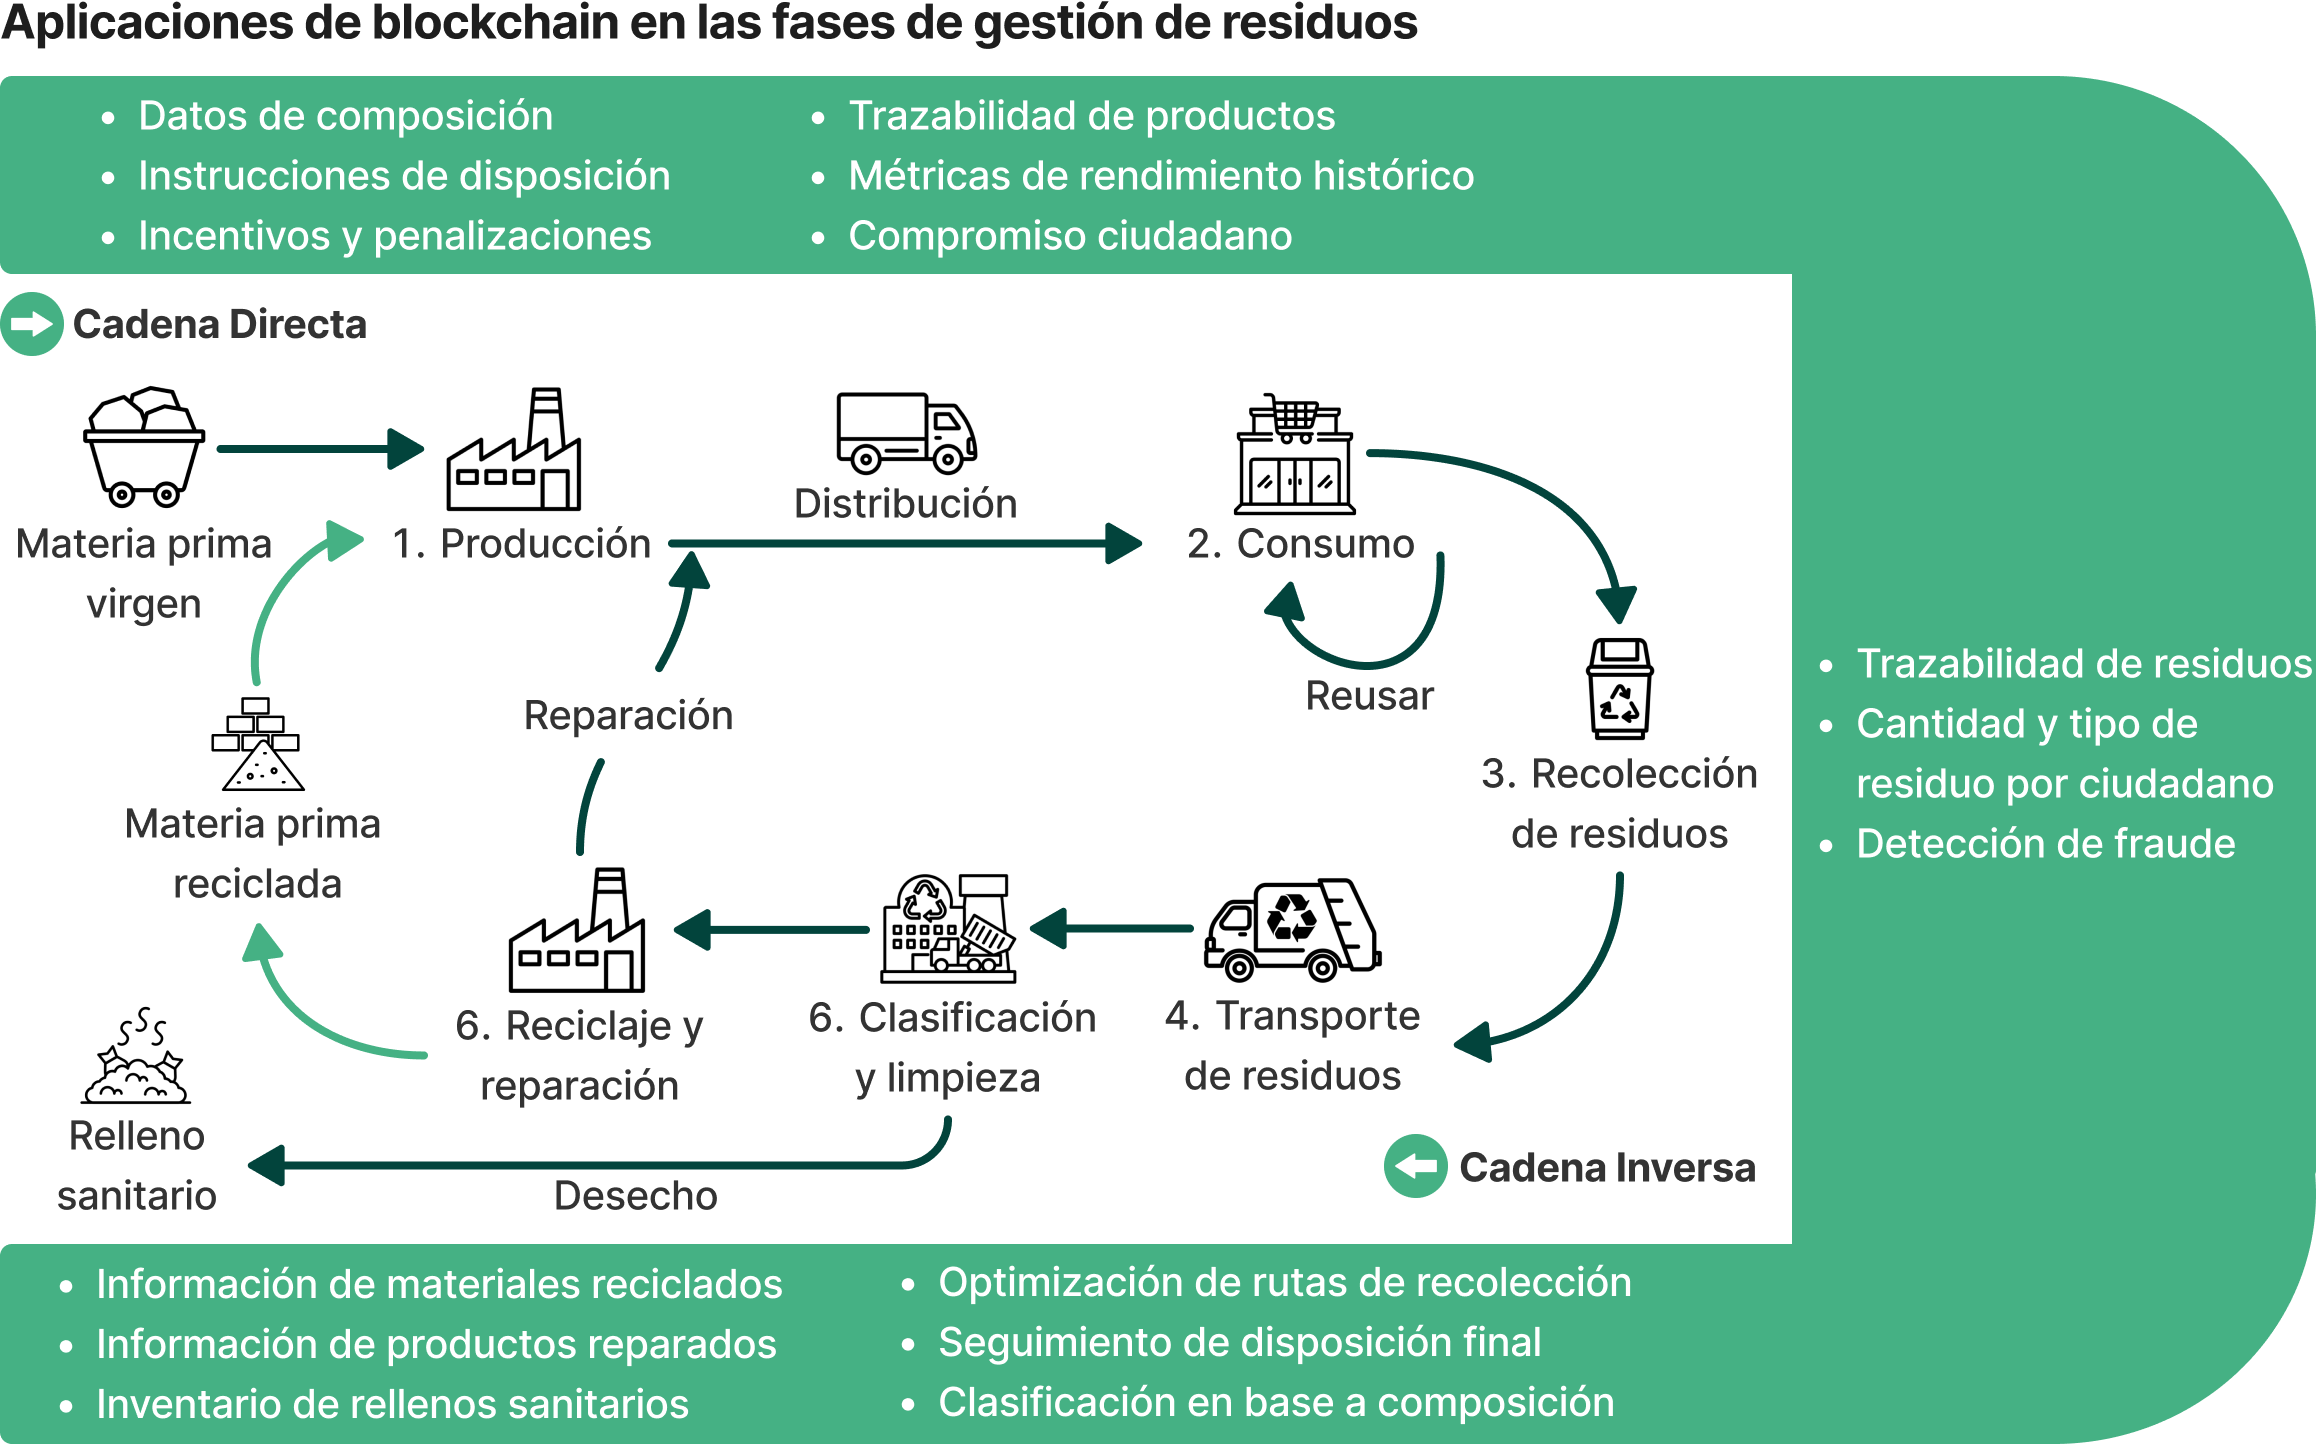
\includegraphics[width=\textwidth]{Figures/baralla-model-1.png}
    \caption[Usos de la tecnología blockchain en la economía circular]{Usos de la tecnología blockchain en las etapas de la economía circular \cite{baralla2023waste}}
    \label{fig:baralla-model-1}
\end{figure}

El proceso de reciclaje varía en complejidad dependiendo del material. Existen diversos materiales reciclables, cada uno con características particulares. El papel y cartón son ampliamente reciclados y fáciles de recolectar, mientras que los metales (como el aluminio, el acero o el cobre) conservan sus propiedades tras múltiples ciclos. Los residuos electrónicos presentan un alto valor por su contenido en metales preciosos, aunque requieren procesos especializados para su desmontaje. Los plásticos representan un desafío por su heterogeneidad, pero pueden reciclarse eficientemente si se rediseñan los envases y se simplifican sus composiciones. Los residuos orgánicos son compostables o pueden aprovecharse energéticamente en caso de no mezclarse con residuos no reciclables. Finalmente, el vidrio destaca como el material circular por excelencia: puede reciclarse infinitas veces sin perder calidad, su estructura es químicamente estable, y su reciclaje requiere menos energía que su producción original. Estas cualidades lo convierten en un insumo ideal para sistemas de economía circular bien diseñados.

\subsection{Cadena de suministro del vidrio}
\label{sec:glass-supply-chain}

El vidrio es uno de los materiales más representativos de la economía circular por su capacidad única de ser reciclado indefinidamente sin perder calidad. Esta propiedad lo convierte en un recurso estratégico para reducir la demanda de materias primas vírgenes, minimizar residuos y disminuir la huella de carbono asociada a la producción industrial. A diferencia de otros materiales cuyo reciclaje implica degradación, el vidrio conserva íntegramente sus características físicas y químicas, permitiendo su reintegración al ciclo productivo tantas veces como sea necesario. En la Figura \ref{fig:glass-lifecycle} se muestra el ciclo de vida del vidrio en un modelo de economía circular, que abarca desde la extracción de materias primas hasta su reincorporación como materia prima en nuevos productos, ejemplificando el caso de los envases de vidrio.

\begin{figure}[!tb]
    \centering
    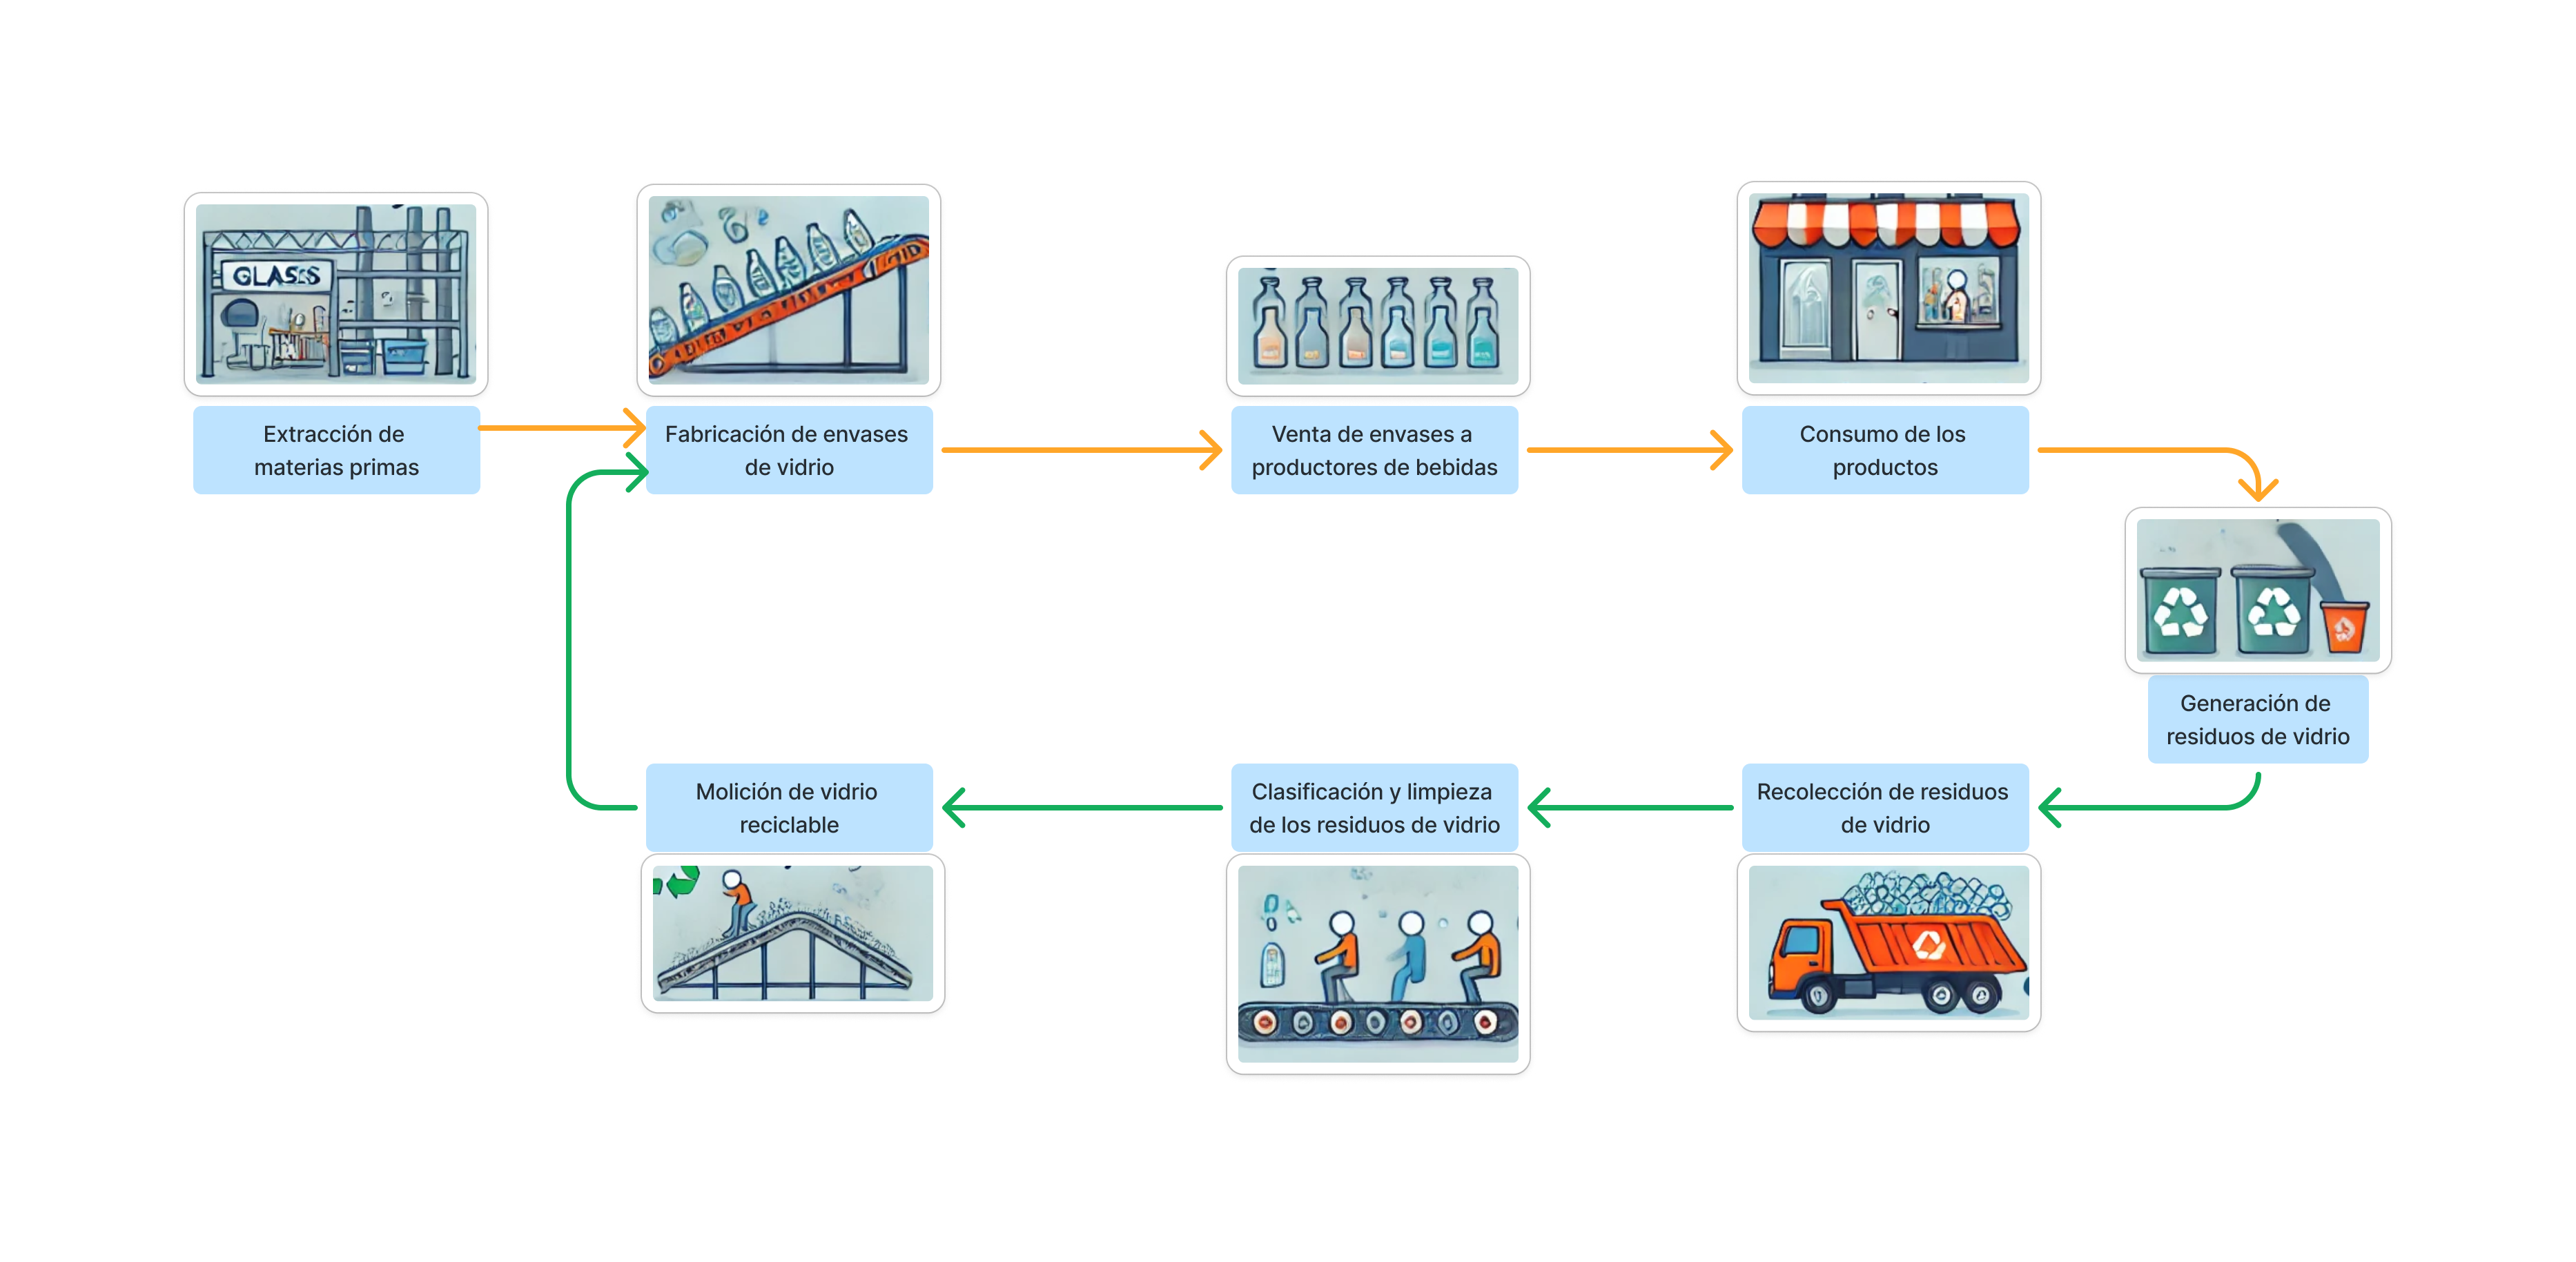
\includegraphics[width=\textwidth]{Figures/glass-lifecycle.png}
    \caption{Ciclo de vida de envases de vidrio en un modelo de economía circular}
    \label{fig:glass-lifecycle}
\end{figure}

% TODO: consider rewriting this with verallia steps listing (tex/theoretical-framework.tex)

El proceso comienza con el diseño del producto, etapa clave para asegurar su durabilidad, reutilización y posterior reciclabilidad. Por ejemplo, en la producción de envases de vidrio, en esta etapa se deciden aspectos como color, forma y composición del envase para optimizar durabilidad, reciclabilidad y aspectos estéticos. Luego del diseño, sigue la producción industrial, donde se funden arena, sosa y caliza a altas temperaturas, frecuentemente combinadas con calcín (vidrio reciclado triturado) para reducir el consumo energético y demanda de materiales vírgenes. La especial reciclabilidad del vidrio se hace visible en esta etapa, ya que la calidad del vidrio resultante es la misma sin importar la proporción de calcín y de materiales vírgenes utilizados (característica que, por ejemplo, no es igual para el plástico), por lo que los productores de vidrio no encuentran pérdidas potenciales al utilizar materiales reciclados. Luego, los envases fabricados son distribuidos, utilizados para embotellar bebidas (por ejemplo, vino) y adquiridos por los consumidores, quienes (luego de consumir su contenido) pueden reutilizarlos, descartarlos (como basura común) o ingresarlos a circuitos de reciclaje. Para el correcto reciclaje del vidrio (y otros materiales) es importante el circuito de recolección diferenciada, que evita que el vidrio reciclable se mezcle con otros materiales que lo contaminen e imposibiliten su reciclaje. Los residuos de vidrio son recolectados por empresas especializadas o por los propios consumidores, quienes pueden depositarlos en contenedores específicos para su posterior tratamiento.
Una vez recolectado, el vidrio es transportado a plantas de reciclaje donde se clasifica. En la clasificación se separa al vidrio de otros materiales reciclables que puedan haber sido mezclados y se separan los distintos tipos de vidrio (por ejemplo, por color), ya que algunas características, como el color y la composición química, son relevantes para el posterior uso del vidrio reciclado. Luego, el vidrio es triturado y limpiado para eliminar impurezas, como etiquetas o restos de alimentos, dando como resultado lo que se conoce como calcín. Esta etapa es crucial, ya que la pureza del material reciclado influye directamente en la calidad del vidrio producido. Finalmente, el calcín se funde nuevamente y se convierte en materia prima para nuevos envases, cerrando así el ciclo de vida del vidrio. Este proceso de reciclaje puede repetirse indefinidamente, lo que lo convierte en un modelo ejemplar de economía circular.

La cadena de suministros y reciclaje de envases de vidrio tiene una importancia estratégica en la provincia de Mendoza, por su estrecha vinculación con la industria vitivinícola, uno de los principales motores económicos de la región. La provincia cuenta con una única empresa que produce y recicla envases de vidrio a escala industrial: Verallia \footnote{\url{https://ar.verallia.com/}}. Esta compañía internacional cubre la totalidad de la demanda local de botellas y frascos, fabricando envases para vinos, espumantes, cervezas, licores y alimentos. El proceso de producción en Verallia incluye desde la selección y mezcla de materias primas hasta la formación, inspección y distribución de los envases, con la integración progresiva de vidrio reciclado como parte del insumo.

Verallia ha reconocido públicamente que la mayor dificultad de su industria es la elevada emisión de dióxido de carbono, por lo que ha adoptado una estrategia dual orientada a optimizar el reciclaje y fomentar la reutilización del vidrio. Bajo esta lógica, ha desarrollado el programa ``Vidrio, una acción transparente`` en alianza con el Gobierno de Mendoza, mediante el cual se promueve la recolección de envases descartados, destinando los ingresos generados al apoyo de organizaciones benéficas. Esta iniciativa, aunque aún incipiente, representa un esfuerzo por avanzar hacia una cadena de suministro más circular y socialmente responsable en la provincia.

Sin embargo, el reciclaje de vidrio en Mendoza enfrenta desafíos estructurales. La tasa de recuperación aún es baja, las métricas oficiales son escasas y las políticas de incentivo son limitadas. La logística de recolección depende en gran medida de la voluntad ciudadana y carece de sistemas obligatorios o premiantes que aseguren su masividad. En este contexto, el rol de actores industriales como Verallia resulta central para impulsar transformaciones sostenibles en la cadena del vidrio, tanto mediante la innovación tecnológica como a través de la articulación público-privada.

Más allá del caso mendocino, el vidrio sigue siendo uno de los materiales más valiosos dentro de una economía circular bien implementada. Su durabilidad, estabilidad química, transparencia y capacidad de reciclaje total lo convierten en un insumo ideal para cerrar ciclos productivos sin pérdidas de calidad ni de valor. Avanzar hacia una cadena del vidrio plenamente circular requiere optimizar cada etapa, desde el diseño y la fabricación hasta la trazabilidad del reciclaje, consolidando sistemas logísticos eficientes, ciudadanos comprometidos y políticas públicas robustas que garanticen su sostenibilidad a largo plazo. En este contexto, la incorporación de sistemas basados en tecnología blockchain ofrece la posibilidad de reforzar la trazabilidad a lo largo de toda la cadena de suministro, facilitando un uso más eficiente y seguro de la información en cada etapa. Esta integración no solo optimiza la operación de cada parte involucrada, sino que también impulsa la adopción de prácticas de economía circular y el uso de blockchain en la región. Tomando esta iniciativa como base para el proyecto, a continuación se detallan proyectos y trabajos previos que han explorado la trazabilidad y el reciclaje de vidrio, así como otras iniciativas vinculadas a la economía circular y la sostenibilidad, las cuales aportan soluciones innovadoras para la gestión de residuos y la promoción de prácticas responsables en la cadena de suministro.

\section{Proyectos y Trabajos Relacionados}
\label{sec:related-work}

La tecnología blockchain se ha posicionado como una herramienta poderosa para mejorar la trazabilidad en cadenas de suministro, ofreciendo registros inmutables y transparentes que permiten rastrear el movimiento de productos desde su origen hasta el consumidor final. Esta característica fortalece la confianza entre los actores y favorece la economía circular, al garantizar la autenticidad e integridad de la información. Numerosos proyectos, tanto comerciales como académicos, han explorado su aplicación en la gestión de residuos y en la trazabilidad de materiales. A continuación, se presentan casos representativos, agrupados por tipología, con sus características, beneficios y limitaciones, a fin de identificar lecciones aplicables al desarrollo de un sistema de trazabilidad para el vidrio.

Entre las soluciones comerciales destaca Signeblock (España) \cite{signeblock2024} con su producto Gouze, que permite registrar cada paso de los procesos productivos y de distribución en blockchain, ofreciendo acceso personalizado a la información mediante un gestor documental unificado. Incorpora digitalización y notarización de procesos, certificación blockchain para garantizar inalterabilidad y códigos QR para compartir información del proceso con consumidores. Sus principales limitaciones se relacionan con la interoperabilidad con sistemas existentes y la resistencia organizacional a compartir datos entre actores. Otra solución relevante es Circularise (Países Bajos) \cite{circularise2024}, plataforma que ofrece pasaportes digitales de productos para trazabilidad de extremo a extremo y el intercambio seguro de datos. Para cada producto registra origen, composición y datos ambientales respaldados por blockchain, facilitando cálculo de huella de carbono. Integra con sistemas ERP y promueve un enfoque abierto e interoperable, utilizando una blockchain pública descentralizada para asegurar credibilidad. Por su parte, Circulor (Reino Unido) \cite{circulor2024} es una plataforma que proporciona trazabilidad completa desde la fuente hasta el consumidor final, ayudando a demostrar procedencia responsable, reducir emisiones y gestionar riesgos. Se integra con plataformas empresariales mediante APIs, rastrea materias primas y controla el flujo de materiales en la producción. En conjunto, estas plataformas evidencian la viabilidad de blockchain para trazabilidad industrial a gran escala, integrando datos ambientales y de origen. No obstante, su enfoque en cadenas de alto valor agregado plantea dudas sobre su adaptación a cadenas de reciclaje de vidrio con márgenes reducidos y mayor fragmentación de actores.

En el ámbito académico, Baralla et al. en su trabajo ``Waste Management: A Comprehensive State of the Art about the Rise of Blockchain Technology'' \cite{baralla2023waste} exploran la trazabilidad de residuos, prevención de fraude e incentivos mediante contratos inteligentes. El modelo planteado permite gestionar tanto la cadena directa (producción y consumo) como la inversa (reciclaje), pero señala la necesidad de enfocarse en categorías específicas de residuos y advierte sobre desafíos de escalabilidad, privacidad y rendimiento en blockchains públicas. 

Otro caso académico es el Modelo ZERO de Sandhiya et al. \cite{sandhiya2020investigating} para reciclaje de plásticos, que integra códigos QR, IoT y blockchain para proveer un sistema de trazabilidad inmutable y brindar incentivos para reciclar a los consumidores. En este modelo, cada producto lleva un QR único grabado molecularmente, evitando manipulaciones, y se utilizan ``bines inteligentes'' que aceptan solo plásticos válidos, con verificación y clasificación automática en máquinas de reciclaje. El modelo ofrece incentivos monetarios a los consumidores y busca mejorar calidad, transparencia y costos del reciclaje. De forma complementaria, Bhubalan et al. \cite{BHUBALAN2022113631} proponen integrar blockchain con marcadores moleculares para rediseñar químicamente plásticos y lograr un reciclaje cerrado. Aunque reconocen su potencial técnico, cuestionan la rentabilidad para plásticos de un solo uso debido a los altos costos de implementación. Estos trabajos demuestran que blockchain puede integrarse con tecnologías de identificación física para reforzar la trazabilidad, pero el nivel de infraestructura requerida puede limitar su adopción en contextos con recursos más restringidos, como el reciclaje de vidrio en entornos municipales o regionales. A su vez, la lógica de incentivar al consumidor mediante un mecanismo verificable y confiable, presente en el Modelo ZERO, encuentra un ejemplo real y ampliamente adoptado en el sistema PFAND en Alemania. Este sistema de Depósito y Reembolso (DRS) no emplea blockchain, pero materializa en la práctica el principio fundamental de estos trabajos: ofrecer una recompensa directa y comprobable para asegurar que el material reciclable retorne a la cadena de valor.

La efectividad de este enfoque se confirma con múltiples experiencias regionales e internacionales, que demuestran que la incorporación de incentivos tangibles es un factor clave para fomentar hábitos de reciclaje en los consumidores e impulsar el desarrollo de una economía circular. En España, Reciclos \cite{reciclos2024} ofrece recompensas por el reciclaje de latas y botellas. En Argentina, Colmena \cite{colmena2024} premia a los usuarios con la criptomoneda JellyCoin, mientras que Greenly Points \cite{greenlypoints2024} en Mendoza otorga puntos canjeables por beneficios locales al entregar residuos reciclables en puntos verdes. A nivel global, Plastic Bank en Canadá utiliza la tecnología blockchain para ofrecer criptomonedas como incentivo a los recolectores de plástico en regiones empobrecidas, demostrando cómo las recompensas digitales pueden impulsar la participación y aumentar la transparencia en el flujo de residuos. Estas experiencias subrayan que, al ofrecer valor a cambio del material reciclable, se logra una mayor involucración ciudadana y se contribuye de manera significativa a cerrar los ciclos de vida de los productos.

Los proyectos y modelos analizados evidencian el vasto potencial de la tecnología blockchain para transformar la gestión de residuos y las cadenas de suministro hacia modelos más sostenibles y circulares. Desde sistemas de incentivos simples hasta plataformas complejas de trazabilidad de extremo a extremo, la inmutabilidad, transparencia y descentralización de blockchain ofrecen soluciones prometedoras. No obstante, se identifican puntos débiles recurrentes en su aplicación actual, que incluyen la necesidad de un mayor desarrollo técnico y madurez de la tecnología, la superación de barreras organizacionales (como la reticencia a compartir datos), los altos costos de implementación inicial, problemas de escalabilidad en redes públicas y el consumo energético en ciertos algoritmos de consenso, así como la aún incipiente regulación y falta de estándares comunes. Es en este contexto de desafíos y oportunidades donde se posiciona el presente trabajo de tesis. A pesar de los avances y el reconocimiento de la importancia del reciclaje de vidrio, especialmente en regiones como Mendoza con una fuerte industria vitivinícola, se observa una fuerte desconexión entre los actores de la cadena de suministro, baja tasa de recuperación (con escasez de métricas oficiales) y débiles políticas de incentivos. Los programas existentes en Argentina, si bien son un paso adelante, aún carecen de mecanismos obligatorios o premiantes que aseguren la masividad de la recolección diferenciada y no garantizan por sí mismos el reciclaje efectivo del material.

Este trabajo busca abordar estas brechas mediante el desarrollo de un prototipo de sistema de trazabilidad del vidrio basado en tecnología blockchain. Enfocado específicamente en la cadena de suministro del vidrio en el contexto mendocino, con el objetivo de integrar a todos los actores del proceso, desde la producción hasta su reintroducción en la cadena de valor. Este sistema se propone permitir el registro y verificación de cada etapa del ciclo de vida del vidrio, mientras que, a su vez, busca superar las limitaciones identificadas en los proyectos preexistentes al ofrecer una solución que facilite la valorización del vidrio, promoviendo una economía circular más transparente, eficiente y sostenible en la región. En este trabajo se hace énfasis en la usabilidad, la integración de datos relevantes y la demostración de los beneficios tangibles para todos los participantes de la cadena.

\chapter[Metodología de trabajo]{Metodología de Trabajo}
\label{cp:methodology}

\parindent0pt

Para la consecución de los objetivos propuestos en este trabajo final, se ha definido una metodología de trabajo que permite planificar y gestionar las diferentes tareas y recursos del proyecto de manera ordenada. Por ello, en este capítulo se presentan los diferentes pasos que se ejecutaron para llegar a cumplir estos objetivos. 

Primeramente, se hablará sobre la planificación del trabajo, haciendo hincapié en las actividades necesarias para llevar a cabo el proyecto de forma ordenada y efectiva (Sección \ref{sec:work-plan}). Posteriormente, se describirá el modelo en V, que es la metodología de desarrollo de software seleccionada como marco de referencia para la organización de las actividades de desarrollo del prototipo tecnológico. Se describirán las etapas del proceso de desarrollo, detallando las actividades y resultados esperados en cada una de ellas a partir de la metodología seleccionada. Finalmente, se profundizará en la gestión del proyecto, haciendo hincapié en las herramientas y prácticas seleccionadas para asegurar una gestión eficiente a lo largo de todas las fases del proceso de desarrollo del prototipo.

\section{Planificación del trabajo}
\label{sec:work-plan}

Definir un plan de trabajo, previo al desarrollo del prototipo tecnológico, es una buena práctica que permite establecer una hoja de ruta concisa que sirve de guía orientativa a lo largo de todo el proceso. El plan de trabajo define los objetivos y actividades necesarios para llevar a cabo un proyecto eficazmente. Para este trabajo en particular, se definió un plan que comprende las actividades necesarias para poder desarrollar un prototipo tecnológico basado en blockchain, orientado a la trazabilidad y valorización del vidrio, con el objetivo de contribuir a la economía circular en la región. Este plan sirve de guía para la ejecución de las actividades y la toma de decisiones a lo largo del proyecto, pero es flexible y puede adaptarse a cambios y nuevas necesidades que puedan surgir durante el desarrollo del trabajo. En la Figura \ref{fig:activities-plan} se ilustran las actividades que conforman el plan de trabajo junto con su duración estimada y secuencialidad. A continuación se detalla el alcance y los objetivos de cada actividad.

\begin{figure}[!htb]
    \centering
    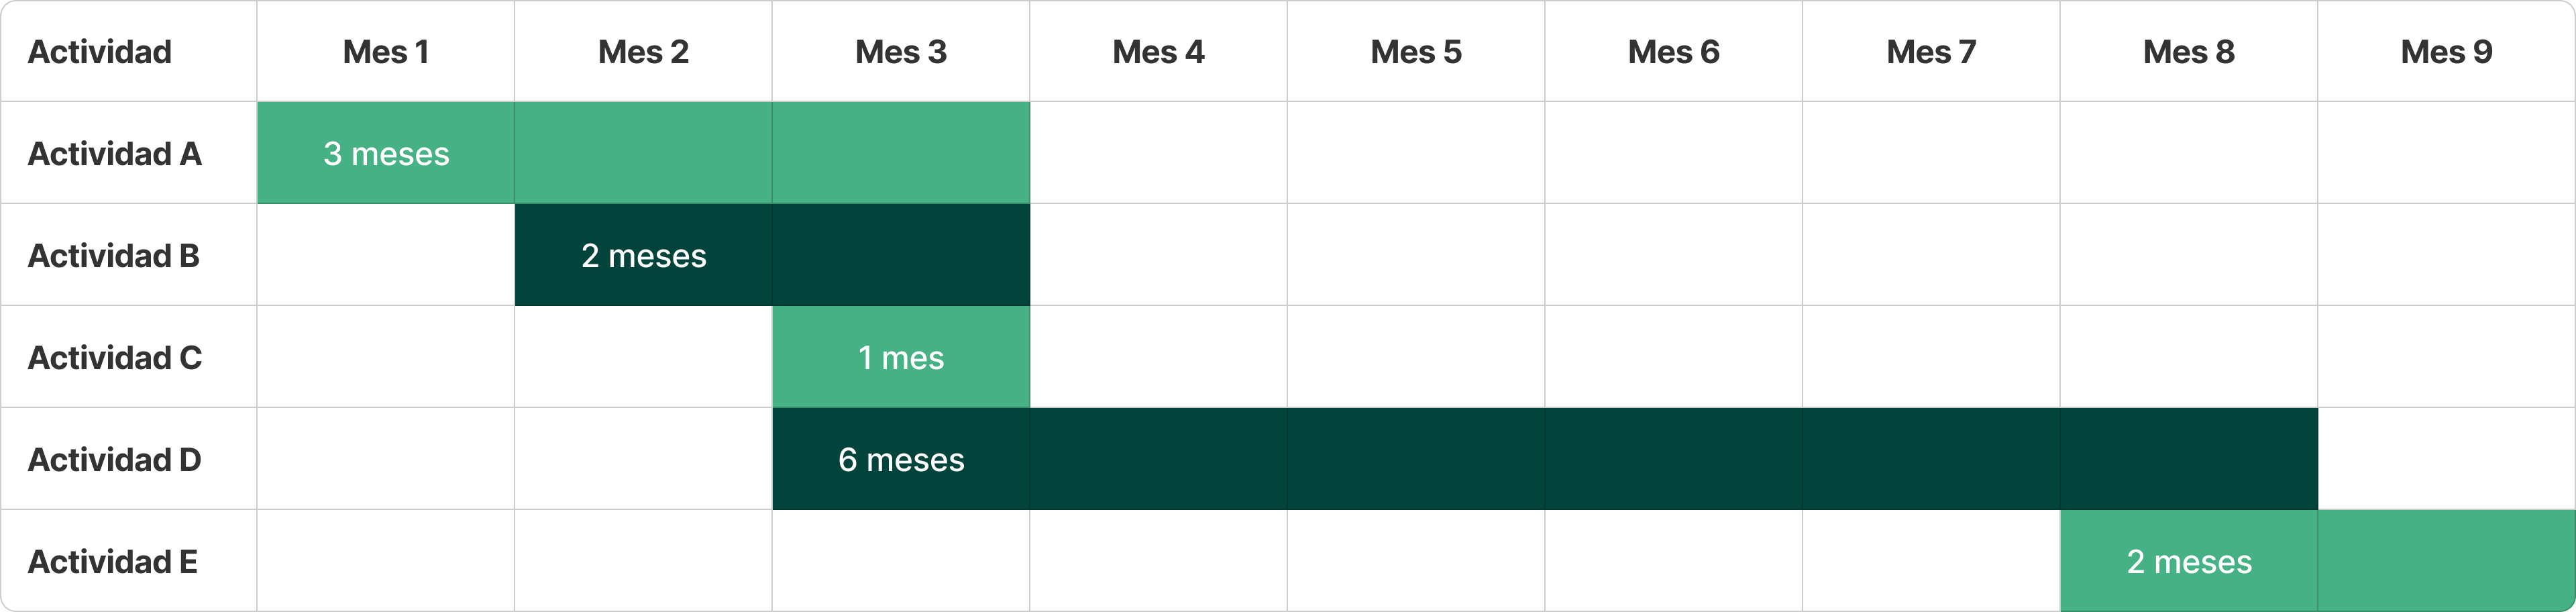
\includegraphics[width=\textwidth]{Figures/activities-plan.png}
    \caption{Organización de las actividades del plan de trabajo}
    \label{fig:activities-plan}
\end{figure}

\begin{itemize}
	\item \textbf{Actividad A}: completar la formación en blockchain y las tecnologías y plataformas relacionadas. Los resultados de esta formación se aplican posteriormente en las etapas de diseño de solución e implementación del prototipo tecnológico (comprendidas en la Actividad D).
	\item \textbf{Actividad B}: realizar un estudio pormenorizado del estado actual del arte en todo lo relacionado con blockchain en el campo del reciclado. En particular, la búsqueda se orienta al reciclado de vidrio. Se analizan trabajos de la literatura, así como aplicaciones blockchain orientadas al reciclaje y la cadena de suministro. Los resultados de este estudio se encuentran documentados en el Capítulo \ref{cp:theoretical-framework}: Marco Teórico y en los Apéndices \ref{cp:verallia-interview}: Entrevista a Verallia y \ref{cp:europe-trip}: Viaje de Investigación.
	\item \textbf{Actividad C}: definir los procesos de desarrollo del prototipo, haciendo hincapié en la aplicación de los fundamentos de la \gls{ingenieriadesoftware} y planificar de forma concisa y clara. En la Sección \ref{sec:software-method} se describe la metodología elegida para el proceso de desarrollo del prototipo tecnológico.
	\item \textbf{Actividad D}: desarrollar la aplicación prototipo. Esta actividad comprende las diferentes etapas del proceso de desarrollo de \gls{software}, desde el análisis de requerimientos, diseño, implementación, validación del prototipo y despliegue. Todos estos pasos se deben ejecutar siguiendo la metodología específica elegida para este trabajo durante la Actividad C, teniendo en cuenta las características particulares del modelo de proceso elegido, con el fin de llevar a cabo el objetivo general de este trabajo.
	\item \textbf{Actividad E}: documentar en una memoria el proceso ejecutado y los resultados del trabajo realizado.
\end{itemize}

La consecución de estas actividades requiere un marco metodológico que permita gestionar el desarrollo del prototipo de manera eficiente. En la siguiente sección, se detallará la metodología de desarrollo de software elegida para este proyecto y se justificarán los motivos de su selección.

\section{Metodología de desarrollo}
\label{sec:software-method}

Para desarrollar un \gls{software} de calidad que cumpla con los objetivos planteados, es necesario seguir una metodología de desarrollo de software que asegure que se sigan buenas prácticas de \gls{ingenieriadesoftware} para poder entregar un producto funcional, estable, documentado y mantenible dentro de los plazos propuestos. Existen diversas metodologías de desarrollo de software que permiten planificar y ordenar el proceso de desarrollo de software para alcanzar los objetivos del proyecto haciendo un uso eficiente de los recursos disponibles. Cada metodología tiene sus propias características, ventajas y desventajas, y la elección de una metodología apropiada depende de las necesidades específicas del proyecto, tales como el alcance del prototipo, la frecuencia de entrega de resultados, la probabilidad de cambios en los requerimientos durante el desarrollo y la estructura del equipo de trabajo.

Las metodologías de desarrollo de software pueden clasificarse en dos grandes categorías: los modelos prescriptivos o tradicionales, que ofrecen una estructura y un orden definidos para maximizar la previsibilidad y la eficiencia en entornos con requerimientos estables, y los modelos evolutivos o ágiles, que se adaptan mejor a las realidades dinámicas del desarrollo de software moderno al permitir la iteración continua y la flexibilidad frente a los cambios \cite{pressman2010ingenieria}. Cada metodología propone una serie de etapas y prácticas que guían el proceso de desarrollo, como pueden ser la definición de requerimientos, el diseño, la implementación, las pruebas, la documentación, el despliegue y el mantenimiento del software.

Particularmente, en este trabajo se debe elegir una metodología de desarrollo de software que sea apropiada para un equipo unipersonal, ya que el desarrollo del prototipo tecnológico es llevado a cabo por una única persona. A su vez, la metodología debe ser adecuada para proyectos con un alcance definido desde el comienzo y con requerimientos relativamente estables, ya que el objetivo del trabajo es desarrollar un prototipo tecnológico funcional que cumpla con los requerimientos planteados inicialmente. Por último, el proyecto tiene una duración limitada con una única entrega del proyecto completo al final, por lo que la metodología debe permitir una planificación clara y concisa para cumplir con los plazos establecidos, aunque debe ser lo suficientemente flexible para adaptarse a cambios menores que puedan surgir durante el desarrollo del prototipo. Teniendo en cuenta estos factores, se decidió adoptar una metodología híbrida para el desarrollo del prototipo que combina el \textit{modelo en V} (tradicional) con la gestión de tareas de \textit{Kanban} (ágil). El modelo en V aporta un enfoque estructurado para la planificación y documentación del proyecto, mientras que Kanban proporciona flexibilidad para la gestión de tareas y el seguimiento del flujo de trabajo diario en un entorno unipersonal.

El modelo en V (Figura \ref{fig:model-v}) es una extensión del \textit{modelo en cascada} que empareja cada fase de desarrollo con una fase de prueba correspondiente \cite{pressman2010ingenieria}. Este modelo propone una estructura de etapas en forma de ``V'', de modo que a medida que el proyecto avanza hacia abajo en la primera mitad de la V, los requerimientos y componentes del sistema son detallados cada vez más hasta llegar a la codificación, de forma similar al funcionamiento del modelo en cascada, donde cada fase debe completarse en orden sin contemplar posibles errores o cambios. Una vez completada la codificación, el proceso asciende por el lado derecho de la V, donde cada etapa de definición anterior es validada a través de pruebas específicas. A diferencia del modelo en cascada, el modelo en V plantea una verificación sistemática en cada etapa, con el fin de detectar y corregir errores de forma temprana y minimizar riesgos al final del proyecto. Este modelo es apropiado para proyectos que requieren altos estándares de calidad y donde los errores tempranos podrían tener consecuencias costosas o críticas. En el caso de un prototipo basado en \glspl{contratointeligente}, la inmutabilidad de los contratos desplegados en la blockchain hace que la detección temprana de errores sea crítica para garantizar la calidad y la fiabilidad del prototipo final, ya que una vez desplegados, los contratos no pueden ser modificados para resolver errores o vulnerabilidades de seguridad.

\begin{figure}[!tb]
	\centering
	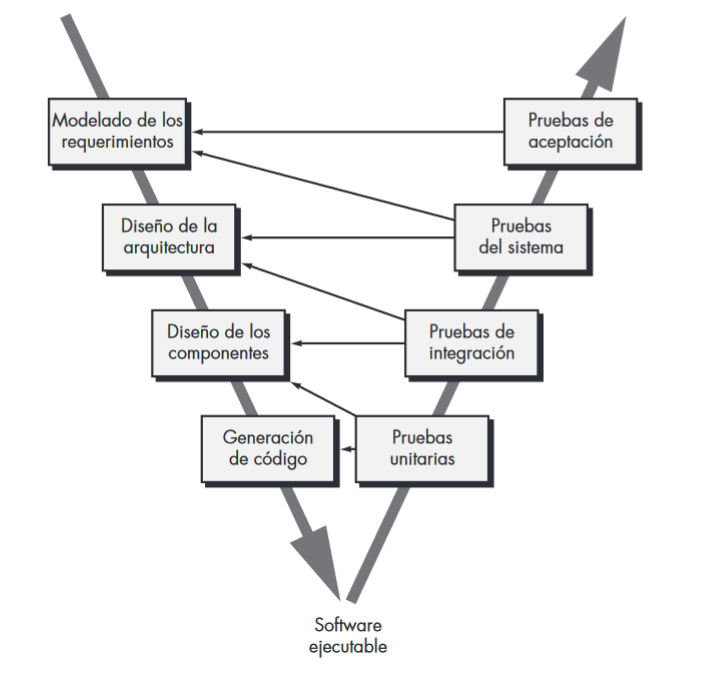
\includegraphics[width=0.6\textwidth]{Figures/model-v.png}
	\caption[Modelo en V]{Modelo en V. Fuente: \cite{pressman2010ingenieria}}
    \label{fig:model-v}
\end{figure}

Por otro lado, el método Kanban es un enfoque visual ágil para la gestión del flujo de trabajo, cuyo objetivo principal es optimizar la eficiencia al prevenir la sobrecarga de tareas y eliminar cuellos de botella \cite{alaidaros2021kanban}. Este método propone implementar un tablero visual dividido en columnas que representan las diferentes etapas del proceso de desarrollo, por donde se mueven las tareas o tarjetas. En la Figura \ref{fig:kanban-board} se muestra un ejemplo de un tablero Kanban para un proyecto en curso. Los principios de este modelo incluyen limitar el trabajo en curso, visualizar el flujo de tareas y medir su progreso para reconocer oportunidades de mejora. Kanban es una metodología ligera que se adapta bien a la situación de cualquier proyecto, es compatible con otras metodologías de trabajo y su implementación no requiere cambios estructurales en el proceso de trabajo. Sin embargo, su eficacia depende de una disciplina rigurosa y una comunicación constante del equipo para asegurar que el flujo visualizado en el tablero refleje la realidad actual del estado del proyecto. La naturaleza visual de Kanban facilita el seguimiento del progreso y permite una adaptación ágil a los cambios menores que puedan surgir en el día a día, sin comprometer la estructura general del proyecto \cite{alaidaros2021kanban}.

\begin{figure}[!tb]
    \centering
    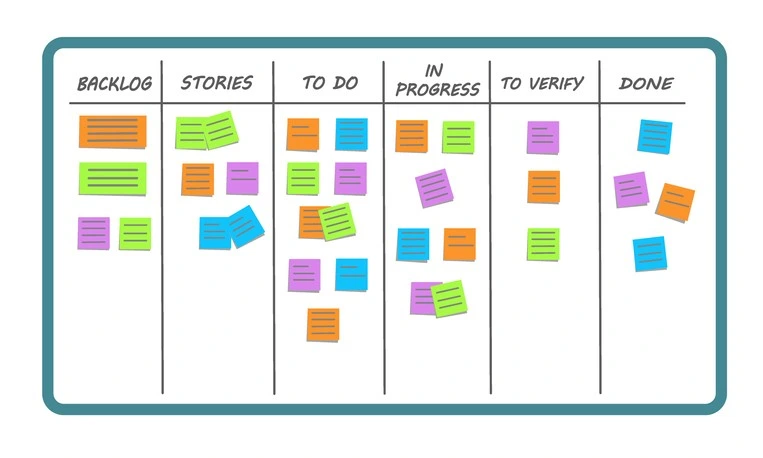
\includegraphics[width=0.9\textwidth]{Figures/model-kanban.png}
    \caption[Tablero Kanban]{Ejemplo de tablero Kanban}
    \label{fig:kanban-board}
\end{figure}

Por su parte, las metodologías ágiles presentan una flexibilidad que las hace adecuadas para proyectos con alta incertidumbre y cambios frecuentes en los requerimientos. Para este proyecto, se desestimó el uso de metodologías ágiles como \textit{Scrum}, ya que su estructura requiere la participación activa de un cliente para guiar reuniones recurrentes para la coordinación del equipo \cite{pressman2010ingenieria}, lo que no es aplicable a un proyecto académico individual. A su vez, el \textit{modelo espiral} es un enfoque iterativo robusto para gestionar riesgos y adaptarse a entornos inciertos \cite{pressman2010ingenieria}, pero tampoco se consideró apropiado para el alcance de este prototipo debido a la complejidad de su proceso evolutivo. En este caso, el proceso resultaría en una sobrecarga innecesaria para el alcance de este prototipo, dado que los requerimientos del trabajo están claramente definidos y la investigación preliminar ha minimizado la incertidumbre en el proceso.

En el contexto del desarrollo de un prototipo tecnológico basado en blockchain, la combinación del modelo en V y Kanban representa la opción más estratégica. El modelo en V proporciona la estructura necesaria para un proyecto con requerimientos estables y una necesidad crítica de alta calidad y fiabilidad. La validación rigurosa que propone este modelo, desde el diseño hasta las pruebas finales, asegura que se detecten y corrijan los errores de forma temprana. Por otro lado, Kanban ofrece flexibilidad operativa para gestionar las tareas del día a día de manera visual, lo que facilita el seguimiento del progreso del proyecto y la adaptación a cambios menores en la planificación.

La elección de esta metodología híbrida busca mantener un enfoque sistemático y estructurado, al mismo tiempo que se aprovecha la flexibilidad operativa en el manejo de tareas diarias. El siguiente apartado abordará en detalle cada etapa del proceso de desarrollo en el contexto del modelo en V, desde el modelado de requerimientos hasta las pruebas, para llevar a cabo el desarrollo del prototipo tecnológico.

\subsection{Etapas del proceso de desarrollo}

Utilizando el modelo en V como marco de referencia, el desarrollo del sistema se concibe como un proceso estructurado que se divide en dos grandes fases: la fase descendente, que se enfoca en la definición, el diseño y la implementación, y la fase ascendente, que se centra en la verificación y las pruebas. A continuación, se detallan las actividades y los resultados esperados de cada una de las etapas del proceso de desarrollo, siguiendo el modelo en V, aplicado al prototipo de trazabilidad del vidrio basado en blockchain. En la Figura \ref{fig:methodology-v-grouped} se muestran las etapas del proceso de desarrollo en V agrupadas en bloques temáticos, con el fin de ilustrar de manera más clara las interacciones y dependencias entre las diferentes fases de desarrollo de este trabajo.

\begin{figure}[!b]
	\centering
	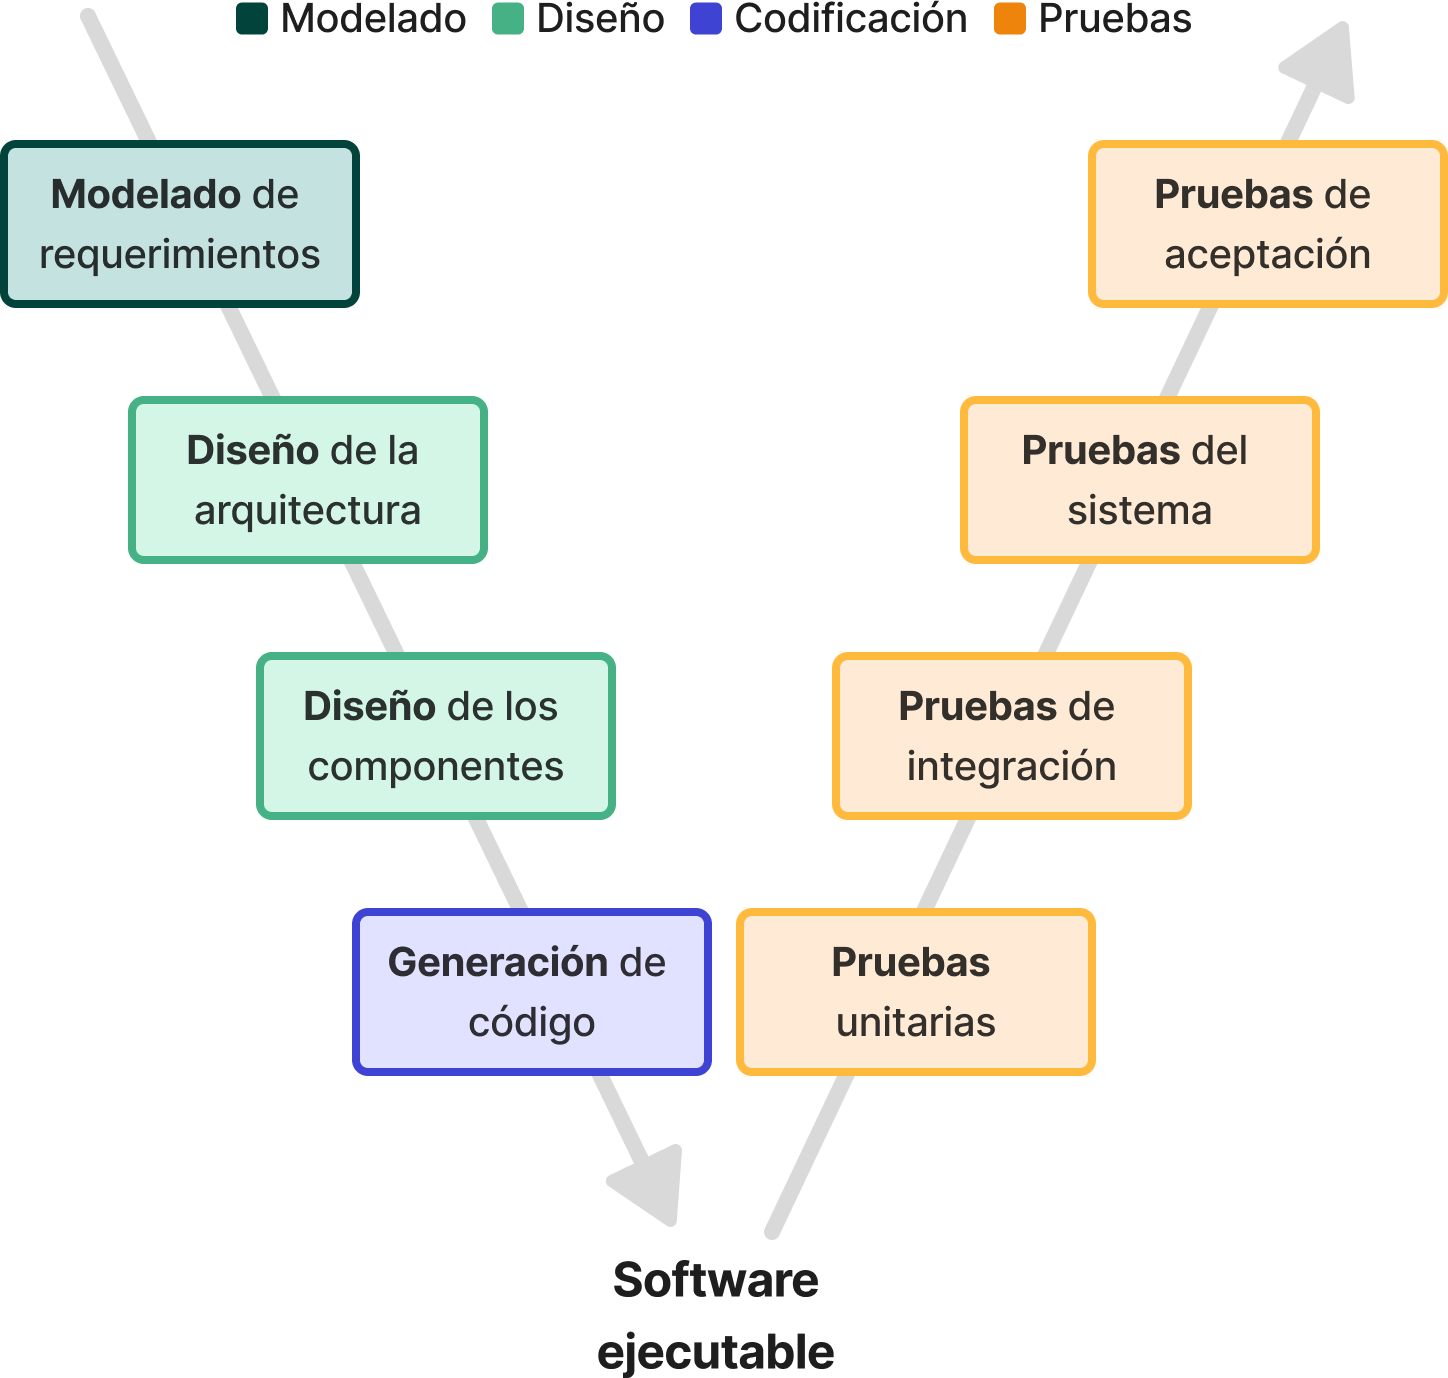
\includegraphics[width=0.6\textwidth]{Figures/model-v-grouped.png}
	\caption{Modelo en V agrupado por etapas}
    \label{fig:methodology-v-grouped}
\end{figure}


\textbf{Modelado de requerimientos:}
Es la primera fase del proceso, comprende la identificación y documentación detallada de los requerimientos funcionales y no funcionales del prototipo.
Los hallazgos se nutren directamente de la investigación realizada como parte de la Actividad B, comprendiendo la revisión del estado del arte en blockchain, gestión de residuos y trazabilidad, así como las entrevistas y las observaciones de programas de reciclaje existentes.
El objetivo en esta etapa es comprender las necesidades específicas del sistema de trazabilidad del vidrio para definir un conjunto exhaustivo de requerimientos que aseguren que el prototipo aborde los desafíos identificados en la cadena de producción de envases de vidrio en la región.
El resultado de esta fase es un documento de requerimientos funcionales y no funcionales que sirve como guía para las siguientes etapas del desarrollo.
La ejecución y resultados de esta fase se detallan en el Capítulo \ref{cp:modelling}.

\textbf{Diseño:}
El diseño del sistema se divide en dos etapas: diseño de arquitectura y diseño de componentes.
En la primera etapa, se define la arquitectura general del sistema, incluyendo la selección de tecnologías y plataformas a utilizar, así como la estructura de los módulos principales y la división de responsabilidades entre ellos.
En la segunda etapa, se realiza el diseño detallado de cada componente de los módulos del sistema, especificando las interfaces, protocolos de comunicación y estructuras de datos a utilizar.
El diseño en etapas y previo a la implementación tiene el objetivo de garantizar que el sistema sea escalable, mantenible y cumpla con los requerimientos definidos en la fase anterior.
El resultado es un conjunto de documentos de diseño que guían la implementación del prototipo. En el Capítulo \ref{cp:design} se presentan los detalles de la ejecución de estas dos fases de diseño del sistema.

\textbf{Generación de código:}
Durante la fase de generación de código o implementación, se lleva a cabo la codificación del prototipo, cada módulo y sus componentes en las tecnologías elegidas y especificaciones detalladas durante la etapa de diseño.
Esta etapa es gestionada con el apoyo de Kanban para la organización y seguimiento de las micro-tareas para mantener un flujo de trabajo ágil y adaptable a los cambios menores que puedan surgir durante el desarrollo.
El resultado de esta fase es un prototipo funcional que implementa los requerimientos y diseños definidos previamente.
En simultáneo con la generación de código se realiza la primera etapa de validación, que consiste en pruebas unitarias de cada componente desarrollado.
Estas pruebas aseguran que cada componente funcione correctamente de forma aislada y cumpla con los requerimientos funcionales especificados.
Al finalizar esta etapa, el software ejecutable está listo para ser desplegado en un entorno de pruebas. El despliegue del prototipo en un entorno de pruebas accesible públicamente (similar a un entorno productivo real) permite evaluar el comportamiento del sistema en condiciones reales y detectar posibles problemas antes de su uso final. A su vez, el entorno de pruebas es necesario para la realización de pruebas de integración y sistema en las etapas posteriores.
Los detalles de la implementación, las pruebas unitarias realizadas y el despliegue se describen en el Capítulo \ref{cp:implementation}.

\textbf{Pruebas:}
El proceso de pruebas se lleva a cabo en múltiples etapas.
Después de las pruebas unitarias, se realizan pruebas de integración automatizadas para verificar que los diferentes módulos del sistema interactúan correctamente entre sí a través de sus interfaces.
Estas pruebas aseguran que los datos fluyan adecuadamente dentro del sistema.
Posteriormente, se llevan a cabo pruebas de sistema para evaluar el comportamiento del prototipo en su conjunto para validar que el sistema cumple con los requerimientos funcionales y no funcionales definidos.
Las pruebas de sistema incluyen pruebas manuales para validar consistencia de datos en el sistema y corroborar que el prototipo cumple con los requerimientos funcionales, junto con pruebas automatizadas mediante código, que permiten verificar los requerimientos no funcionales como rendimiento y seguridad bajo condiciones simuladas.
Finalmente, se realizan pruebas de aceptación con un conjunto de usuarios voluntarios para validar que el prototipo cumple con los criterios de aceptación establecidos en la fase de modelado de requerimientos.
Los detalles de las pruebas realizadas en estas etapas de pruebas se presentan en el Capítulo \ref{cp:testing}.

\section{Gestión del proyecto}

Para asegurar una gestión eficiente a lo largo de todas las fases del proceso de desarrollo es necesario implementar herramientas y prácticas de control de proyectos. La gestión del proyecto comprende la planificación, organización y supervisión de todas las actividades relacionadas con el desarrollo del prototipo, asegurando que se cumplan los plazos, se gestionen los recursos de manera efectiva y se mantenga la calidad del trabajo realizado.

Para la gestión de tareas diarias y el seguimiento del progreso del proyecto mediante Kanban, se decidió hacer uso de la herramienta Jira \footnote{\url{https://www.atlassian.com/es/software/jira}}. Este \gls{software} de gestión de proyectos de desarrollo de software provee una funcionalidad de tablero Kanban y permite gestionar el flujo de trabajo, asignar tareas a los miembros del equipo y realizar un seguimiento del progreso durante el desarrollo a través de una aplicación web con una interfaz intuitiva. 

A su vez, se determinó utilizar el software Git para el control de versiones del código fuente, una herramienta que permite un seguimiento detallado, seguro y ordenado de los cambios en el código. Git permite revertir cambios, comparar versiones y mantener un historial completo de modificaciones del código fuente, lo que permite programar de manera ordenada y segura en caso de problemas que puedan surgir durante el desarrollo. Junto con Git, se utiliza la plataforma GitHub \footnote{\url{https://github.com}}, que permite almacenar y gestionar repositorios de código en la nube, permitiendo el acceso remoto y público al código del proyecto. En el Apéndice \ref{cp:annex-content} se detallan los enlaces a los recursos adicionales relacionados con el proyecto, incluyendo la dirección del repositorio de código fuente en GitHub.

Por otro lado, es necesario definir la estrategia de documentación del proyecto de software previamente al inicio del desarrollo. La documentación forma parte del proceso de desarrollo de software y es un entregable en sí mismo, ya que proporciona una referencia clara y confiable sobre el diseño, la implementación y el uso del sistema para los desarrolladores actuales y futuros del proyecto. En este trabajo, se decidió adoptar una estrategia de documentación continua a lo largo de todas las etapas del proceso de desarrollo. Documentar cada fase del modelo en V, desde la definición de requerimientos hasta las pruebas y el despliegue, asegura que toda la información relevante esté disponible para futuras referencias y facilita la comprensión del sistema por parte de otros desarrolladores o partes interesadas. En el caso del código fuente, se combinan dos enfoques: la documentación mediante comentarios en el código y la documentación externa, que comprende documentos separados dentro del repositorio de código fuente, que describen la arquitectura del sistema, instrucciones de instalación, guías de prueba y cualquier otra información relevante para entender y mantener el código del proyecto.

A partir de la selección de la metodología de desarrollo de software y la estrategia de gestión del proyecto, en los próximos capítulos se presentará el proceso de ejecución llevado a cabo en este trabajo para cada una de las etapas planteadas, incluyendo los resultados obtenidos en cada una.
En el Capítulo \ref{cp:modelling} se describirá el proceso de modelado de requerimientos, donde se explica cómo se obtuvieron los requerimientos funcionales y no funcionales, su priorización y la planificación del desarrollo.
En el Capítulo \ref{cp:design} se abordará el diseño del sistema, incluyendo la elección de tecnologías, diseño de arquitectura de software, modelado de la interfaz de usuario y definición de los módulos principales del prototipo.
Seguidamente, en el Capítulo \ref{cp:implementation} se detallará la implementación de cada módulo del sistema, integración de los módulos, pruebas unitarias realizadas y despliegue del prototipo en un entorno de pruebas similar a un entorno productivo.
En el Capítulo \ref{cp:testing} se describirán las pruebas realizadas, tanto las pruebas de integración automatizadas como las pruebas de sistema manuales y las pruebas con usuarios.
Finalmente, en el Capítulo \ref{cp:conclusions} se presentarán las conclusiones del trabajo, resultados obtenidos, reflexiones sobre el proceso de desarrollo y oportunidades de mejora de este trabajo con recomendaciones para futuros trabajos relacionados con la trazabilidad y valorización del vidrio mediante tecnologías emergentes como blockchain.

\chapter[Modelado de Requerimientos]{Modelado de Requerimientos}
\label{cp:modelling}

\parindent0pt

El modelado de requerimientos constituye la etapa inicial del lado izquierdo del modelo en V, que enfatiza la importancia de las pruebas en cada fase del ciclo de vida del proyecto de software. El objetivo principal de esta etapa es comprender, documentar y validar las necesidades y expectativas de los actores interesados del sistema, definiendo de forma precisa su comportamiento y funcionalidades. Esta fase se asocia directamente con las pruebas de aceptación del lado derecho de la V, la etapa final del modelo, en la cual se verifica que el sistema cumple con los requerimientos definidos inicialmente.

Un modelado de requerimientos preciso incide en las etapas subsiguientes de diseño, implementación y pruebas. Los errores o ambigüedades en la fase de modelado pueden propagarse a lo largo del proyecto, resultando en un aumento del tiempo y los recursos requeridos para corregirlos. Por lo tanto, la inversión de esfuerzo para asegurar que los requerimientos sean claros, completos y factibles reduce el riesgo de inconsistencias y la necesidad de refactorizaciones en fases posteriores, contribuyendo a la ejecución exitosa del proyecto.

En el contexto de este trabajo, centrado en el desarrollo de un prototipo de aplicación con tecnología blockchain para la trazabilidad y valorización de envases de vidrio, el modelado de requerimientos se ejecutó de forma estructurada para garantizar que el prototipo respondiera a las necesidades específicas de una economía circular sostenible y transparente.

El proceso de modelado de requerimientos se estructuró en una serie de pasos iterativos para descubrir, definir y refinar los requisitos del sistema. Las etapas del proceso se resumen en la Figura \ref{fig:requirements-modelling-process}.

\begin{figure}[!htpb]
    \centering
    
\includegraphics[width=0.6\textwidth]{Figures/requirements-modelling.png}
    \caption{Etapas del proceso de modelado de requerimientos del prototipo de trazabilidad de vidrio}
    \label{fig:requirements-modelling-process}
\end{figure}

El proceso dio inicio con una investigación exhaustiva del dominio del problema para identificar los actores clave y sus interacciones (Sección \ref{sec:domain-definition}). A partir de esta información, se elaboró un \textit{Canvas de Propuesta de Valor} para documentar de manera flexible las necesidades y problemáticas de cada actor. Posteriormente, se modelaron los casos de uso para describir las funcionalidades del sistema desde la perspectiva del usuario (Sección \ref{sec:use-cases}). Estos casos de uso constituyeron la base para la definición formal de los requerimientos funcionales y no funcionales, incluyendo sus interdependencias (Sección \ref{sec:requirements-definition}). Finalmente, se redactaron \textit{historias de usuario} con un nivel de detalle suficiente para definir los criterios de aceptación, lo cual permitió iniciar las etapas de diseño de arquitectura, estimación de esfuerzo y planificación de la implementación.

\section{Definición de Dominio}
\label{sec:domain-definition}

El modelado de requerimientos inicia con la definición del dominio del problema. En el contexto de este proyecto, que busca la trazabilidad y valorización del vidrio, el objetivo es comprender el entorno en el que el sistema operará, identificando los actores y sus interacciones. El análisis establece la base para la construcción de los requerimientos del sistema.

La definición del dominio se realizó a través de una investigación y revisión de la literatura sobre la trazabilidad del vidrio. En la Sección \ref{sec:related-work}, se exploraron los trabajos existentes en el área de blockchain aplicada para lograr una economía circular, también se investigaron proyectos existentes que aborden la misma temática o el uso de tecnología para el mismo fin. A su vez, se realizaron entrevistas e investigaciones de campo con expertos en la industria del vidrio y el reciclaje regional, para comprender los procesos actuales, las problemáticas y las expectativas de los actores involucrados (Apéndices \ref{cp:verallia-interview} y \ref{cp:europe-trip}). Se examinaron las etapas del ciclo de vida de los envases de vidrio, desde su producción hasta su reintroducción en la cadena de valor, para identificar los puntos donde la tecnología blockchain puede aplicarse. La Figura \ref{fig:glass-lifecycle-modelling} ilustra el ciclo de vida de los envases de vidrio y los actores involucrados en cada etapa.

\begin{figure}[!htpb]
    \centering
    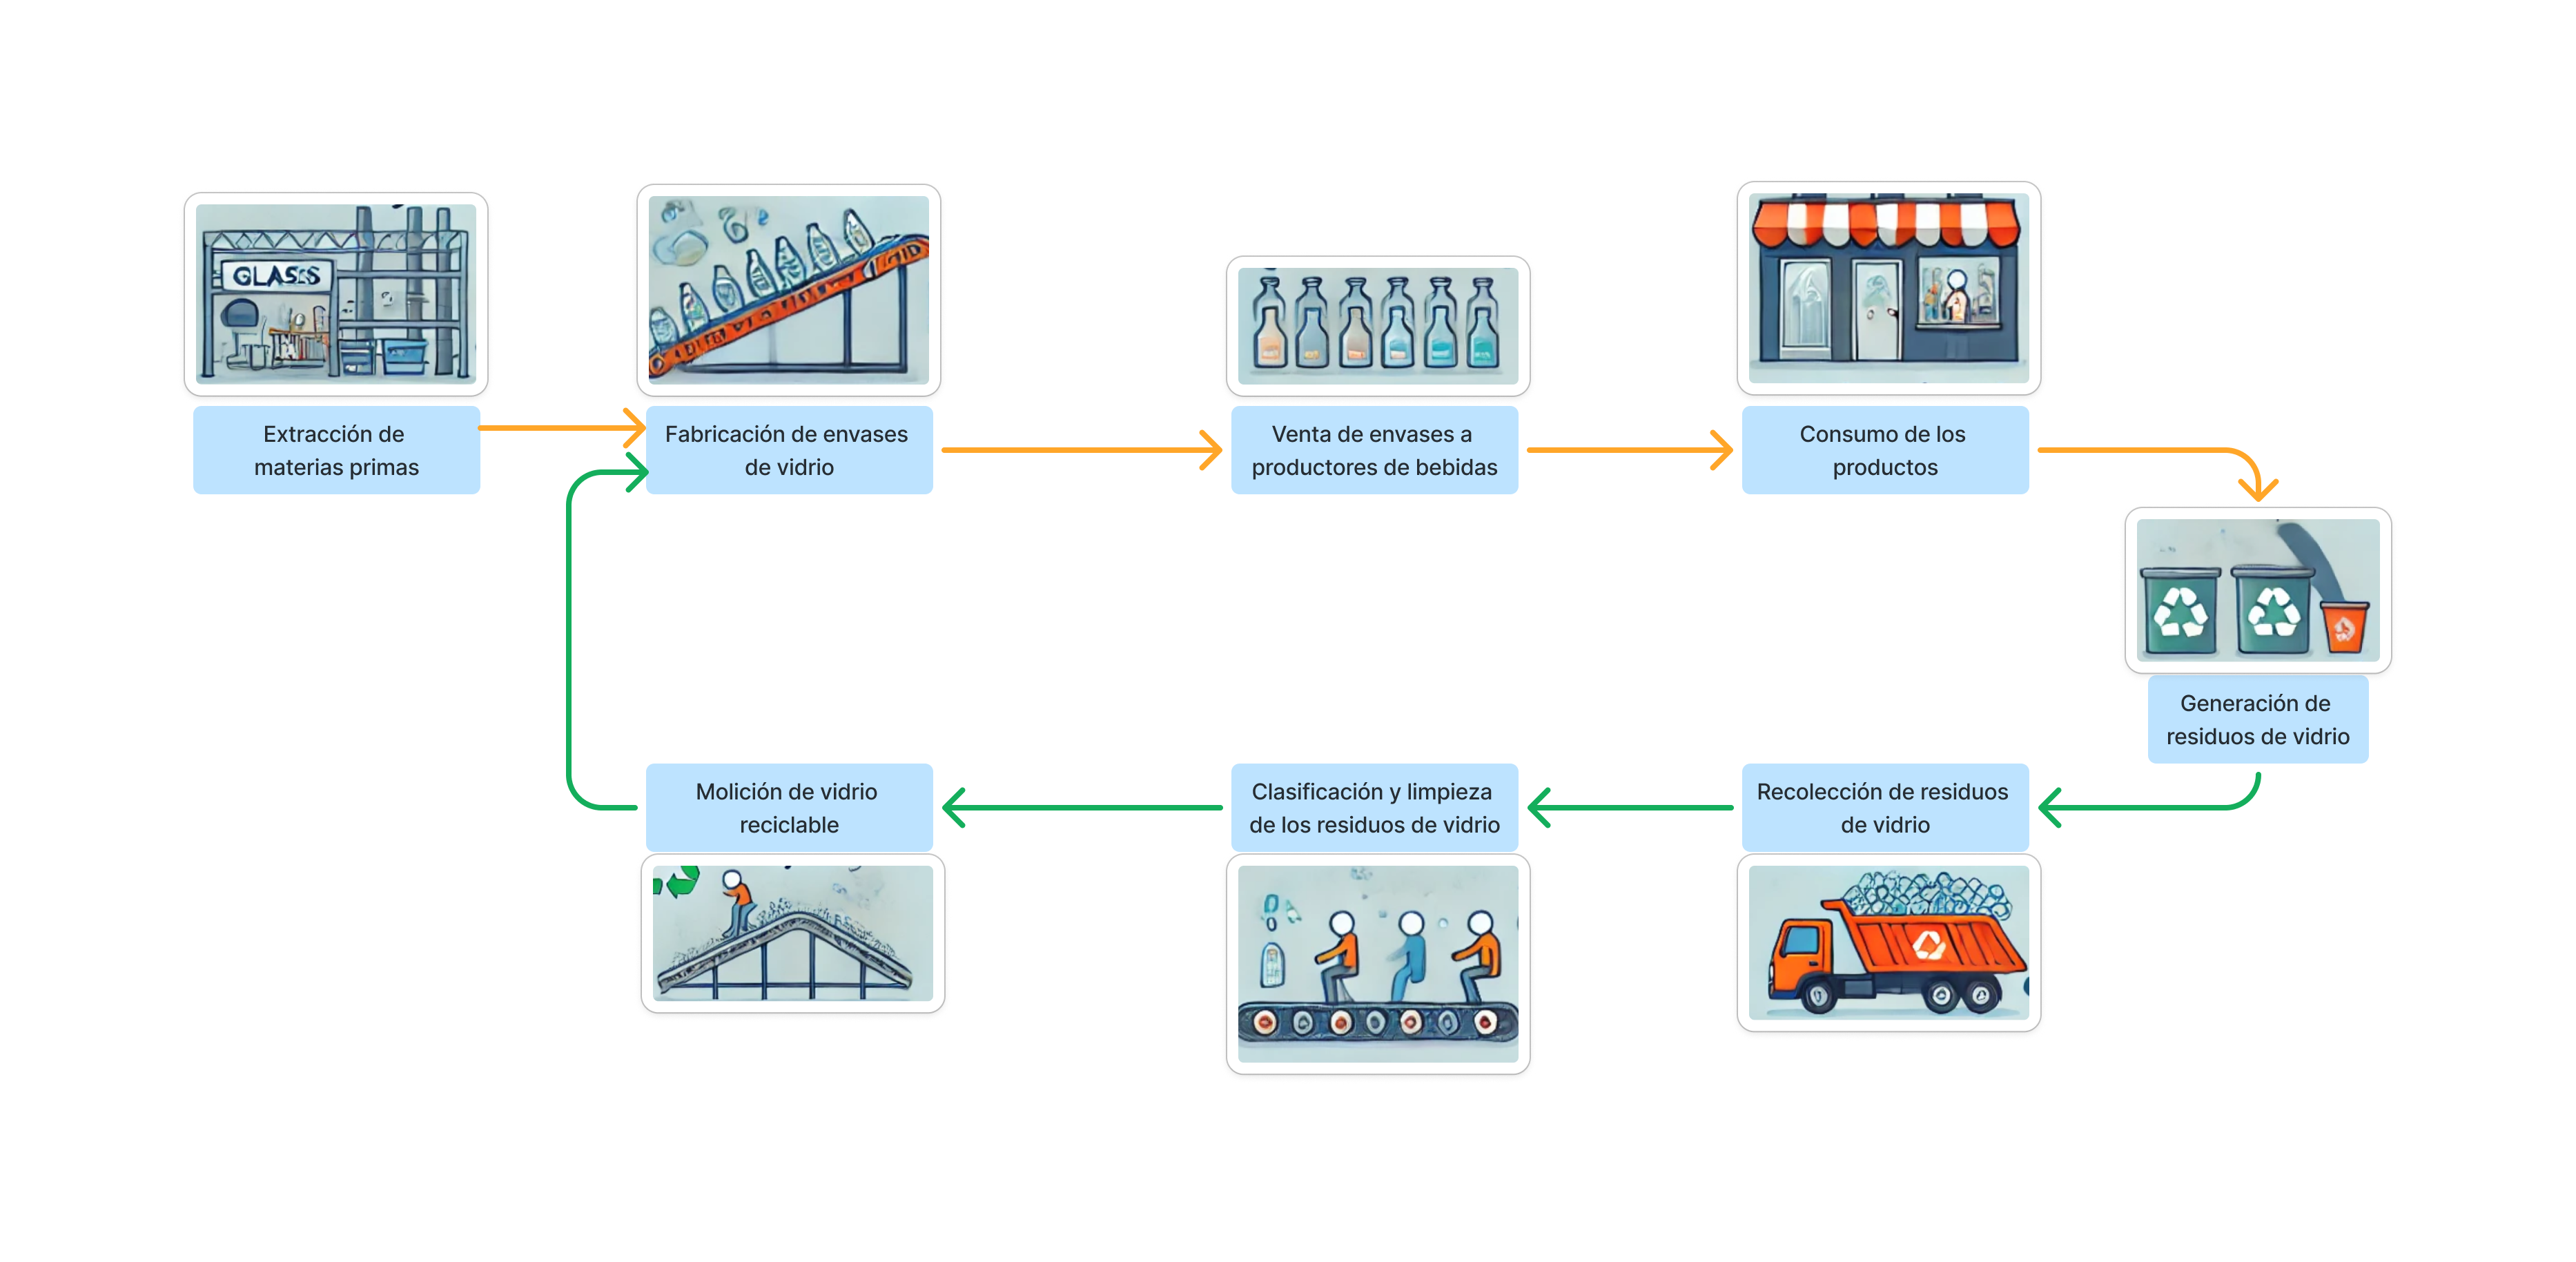
\includegraphics[width=0.6\textwidth]{Figures/glass-lifecycle.png}
    \caption{Etapas del ciclo de vida de los envases de vidrio}
    \label{fig:glass-lifecycle-modelling}
\end{figure}

En este marco, se identificaron los siguientes actores clave:

\begin{itemize}
    \item \textbf{Productor de Vidrio (Productor Primario):} Fabricante del envase de vidrio, con la responsabilidad de registrar la información inicial del lote de material.
    \item \textbf{Productor de vino (Productor Secundario):} Empresa productora de vino que utiliza el envase de vidrio para embotellar sus productos y requiere acceder a la información de trazabilidad con el fin de garantizar la calidad y seguridad alimentaria.
    \item \textbf{Consumidor:} Usuario final que adquiere bebidas envasadas, las consume y puede participar en el proceso de reciclaje.
    \item \textbf{Centro de Reciclaje:} Entidad que recibe, procesa y recicla el vidrio, utiliza la información de trazabilidad para verificar la calidad del material reciclado y dejar registro de su disposición final.
\end{itemize}

Dado que el público objetivo del sistema incluye a todos los actores involucrados en la cadena de valor de los envases de vidrio, se planteó realizar una propuesta de valor que incluya a todos ellos. Tras la identificación de los actores, la revisión de la literatura y la investigación de campo y entrevistas, se elaboró un Canvas de Propuesta de Valor. Este diagrama semi-estructurado es una herramienta estratégica que permite documentar de manera flexible las necesidades y desafíos de cada actor, facilitando la comprensión de sus expectativas.

El canvas se divide en dos secciones principales: el perfil del actor y el mapa de valor de la solución. En el perfil del actor, se detallan sus necesidades, deseos y miedos, lo que proporciona una visión clara de sus motivaciones y los obstáculos que enfrentan en su estado actual. En el mapa de valor de la solución, se definen las funcionalidades y experiencia que ofrecerá la solución, con el objetivo de aplacar los miedos y satisfacer las necesidades y los deseos de los actores. Este análisis conjunto de las expectativas y la solución permite adoptar un enfoque centrado en el usuario desde el inicio del proceso de diseño de solución, asegurando que el sistema propuesto aborde de manera efectiva los problemas y oportunidades identificados.

La Figura \ref{fig:value-proposition-canvas} muestra el canvas elaborado para este sistema de trazabilidad, detallando las necesidades y expectativas de cada actor. Este análisis, al contrastar las necesidades y expectativas de los actores con las funcionalidades de la solución, sirve como el primer paso para conceptualizar cómo el sistema de trazabilidad basado en blockchain puede mitigar los problemas existentes en la cadena de valor de los envases de vidrio y generar valor tangible para cada participante.

\begin{figure}[!htpb]
    \centering
    \includegraphics[width=0.8\textwidth]{Figures/value-proposition-canvas.png}
    \caption{Canvas de Propuesta de Valor para el sistema de trazabilidad de vidrio}
    \label{fig:value-proposition-canvas}
\end{figure}

El análisis detallado a través del Canvas de Propuesta de Valor revela que los principales desafíos se centran en la falta de transparencia y la ineficiencia de los procesos actuales involucrados en el ciclo de vida del vidrio. El Productor Primario necesita un flujo constante de materia prima reciclada de calidad para minimizar sus costos y cumplir con metas de sostenibilidad. A su vez, el Productor Secundario enfrenta el desafío de verificar la procedencia de los envases de vidrio para garantizar la seguridad alimentaria y, de esta manera, acceder a mercados regulados y sostenibles, cumpliendo sus propias metas de sostenibilidad. Por su parte, el Consumidor busca una forma simple de reciclar, con la seguridad de que su esfuerzo es valorado y recompensado, y desea tener la capacidad de conocer el impacto ambiental de los productos que adquiere. Finalmente, el Centro de Reciclaje se enfrenta a altos costos operativos y a falta de calidad en el material recibido, lo que dificulta su valorización. Estas problemáticas y expectativas compartidas se traducen en la necesidad de un sistema unificado y confiable, que permita a los actores verificar la procedencia del material, documentar cada etapa del ciclo de vida y ofrecer incentivos a los usuarios finales. Por lo tanto, los casos de uso del sistema se diseñan para abordar directamente estas necesidades, permitiendo el registro de lotes de producción de envases, consulta de la trazabilidad de cada unidad, gestión del reciclaje de los envases y verificación de la calidad del material reciclado.

% TODO: acá poner las soluciones también, son como una previa a los casos de uso.

La información recopilada en esta fase proporciona una comprensión de las necesidades de los actores y sienta las bases para la siguiente etapa del modelado de requerimientos, donde se definirán los casos de uso del sistema con una perspectiva centrada en el usuario.

\section{Modelado de Casos de Uso}
\label{sec:use-cases}

Después de definir el dominio y los actores, se procede a la identificación y modelado de los casos de uso. Un caso de uso describe una interacción atómica entre un actor y el sistema para alcanzar un objetivo específico, representando una funcionalidad desde la perspectiva del usuario.

Con el objetivo de acotar el alcance de este trabajo, se realiza el modelado de los casos de uso relacionados con la trazabilidad de los envases de vidrio, abarcando las acciones que los actores pueden realizar en el sistema. Estos casos de uso se centran en las funcionalidades esenciales que permiten a los actores registrar, consultar y gestionar la información relacionada con los envases de vidrio a lo largo de su ciclo de vida. Los casos de uso relacionados con la certificación de cada etapa del proceso e integración con sistemas preexistentes se consideran fuera del alcance de este trabajo, pero los casos de uso modelados permiten sentar las bases para futuras extensiones del sistema hacia estas funcionalidades.

En el prototipo de sistema de trazabilidad para envases de vidrio, los casos de uso comprenden tanto las acciones inherentes al ciclo de vida del material como las interacciones propias de una plataforma digital basada en blockchain. Los primeros tipos de caso de uso describen las operaciones fundamentales del proceso de trazabilidad, como el registro de un nuevo lote de envases fabricado por parte del Productor Primario, la consulta del origen del envase por parte del Consumidor y la recepción de envases reciclables por el Centro de Reciclaje. Los segundos tipos de caso de uso, por su parte, abarcan las funcionalidades básicas del sistema, tales como la autenticación de usuarios y la visualización de datos en la interfaz.

Los casos de uso se representan gráficamente a través de un diagrama de casos de uso que muestra las interacciones entre los actores y el sistema. La Figura \ref{fig:use-case-diagram} presenta el diagrama elaborado para el sistema de trazabilidad de envases de vidrio para una economía circular, ilustrando las funcionalidades mínimas que debe implementar el sistema y los actores asociados a cada funcionalidad. Cada caso de uso está vinculado a un actor específico, lo que permite visualizar claramente las interacciones y responsabilidades de cada uno. En caso de que un caso de uso sea compartido por varios actores, se puede representar como un caso de uso heredado, indicando que varios actores pueden realizar la misma acción o funcionalidad.

\begin{figure}[!htpb]
    \centering
    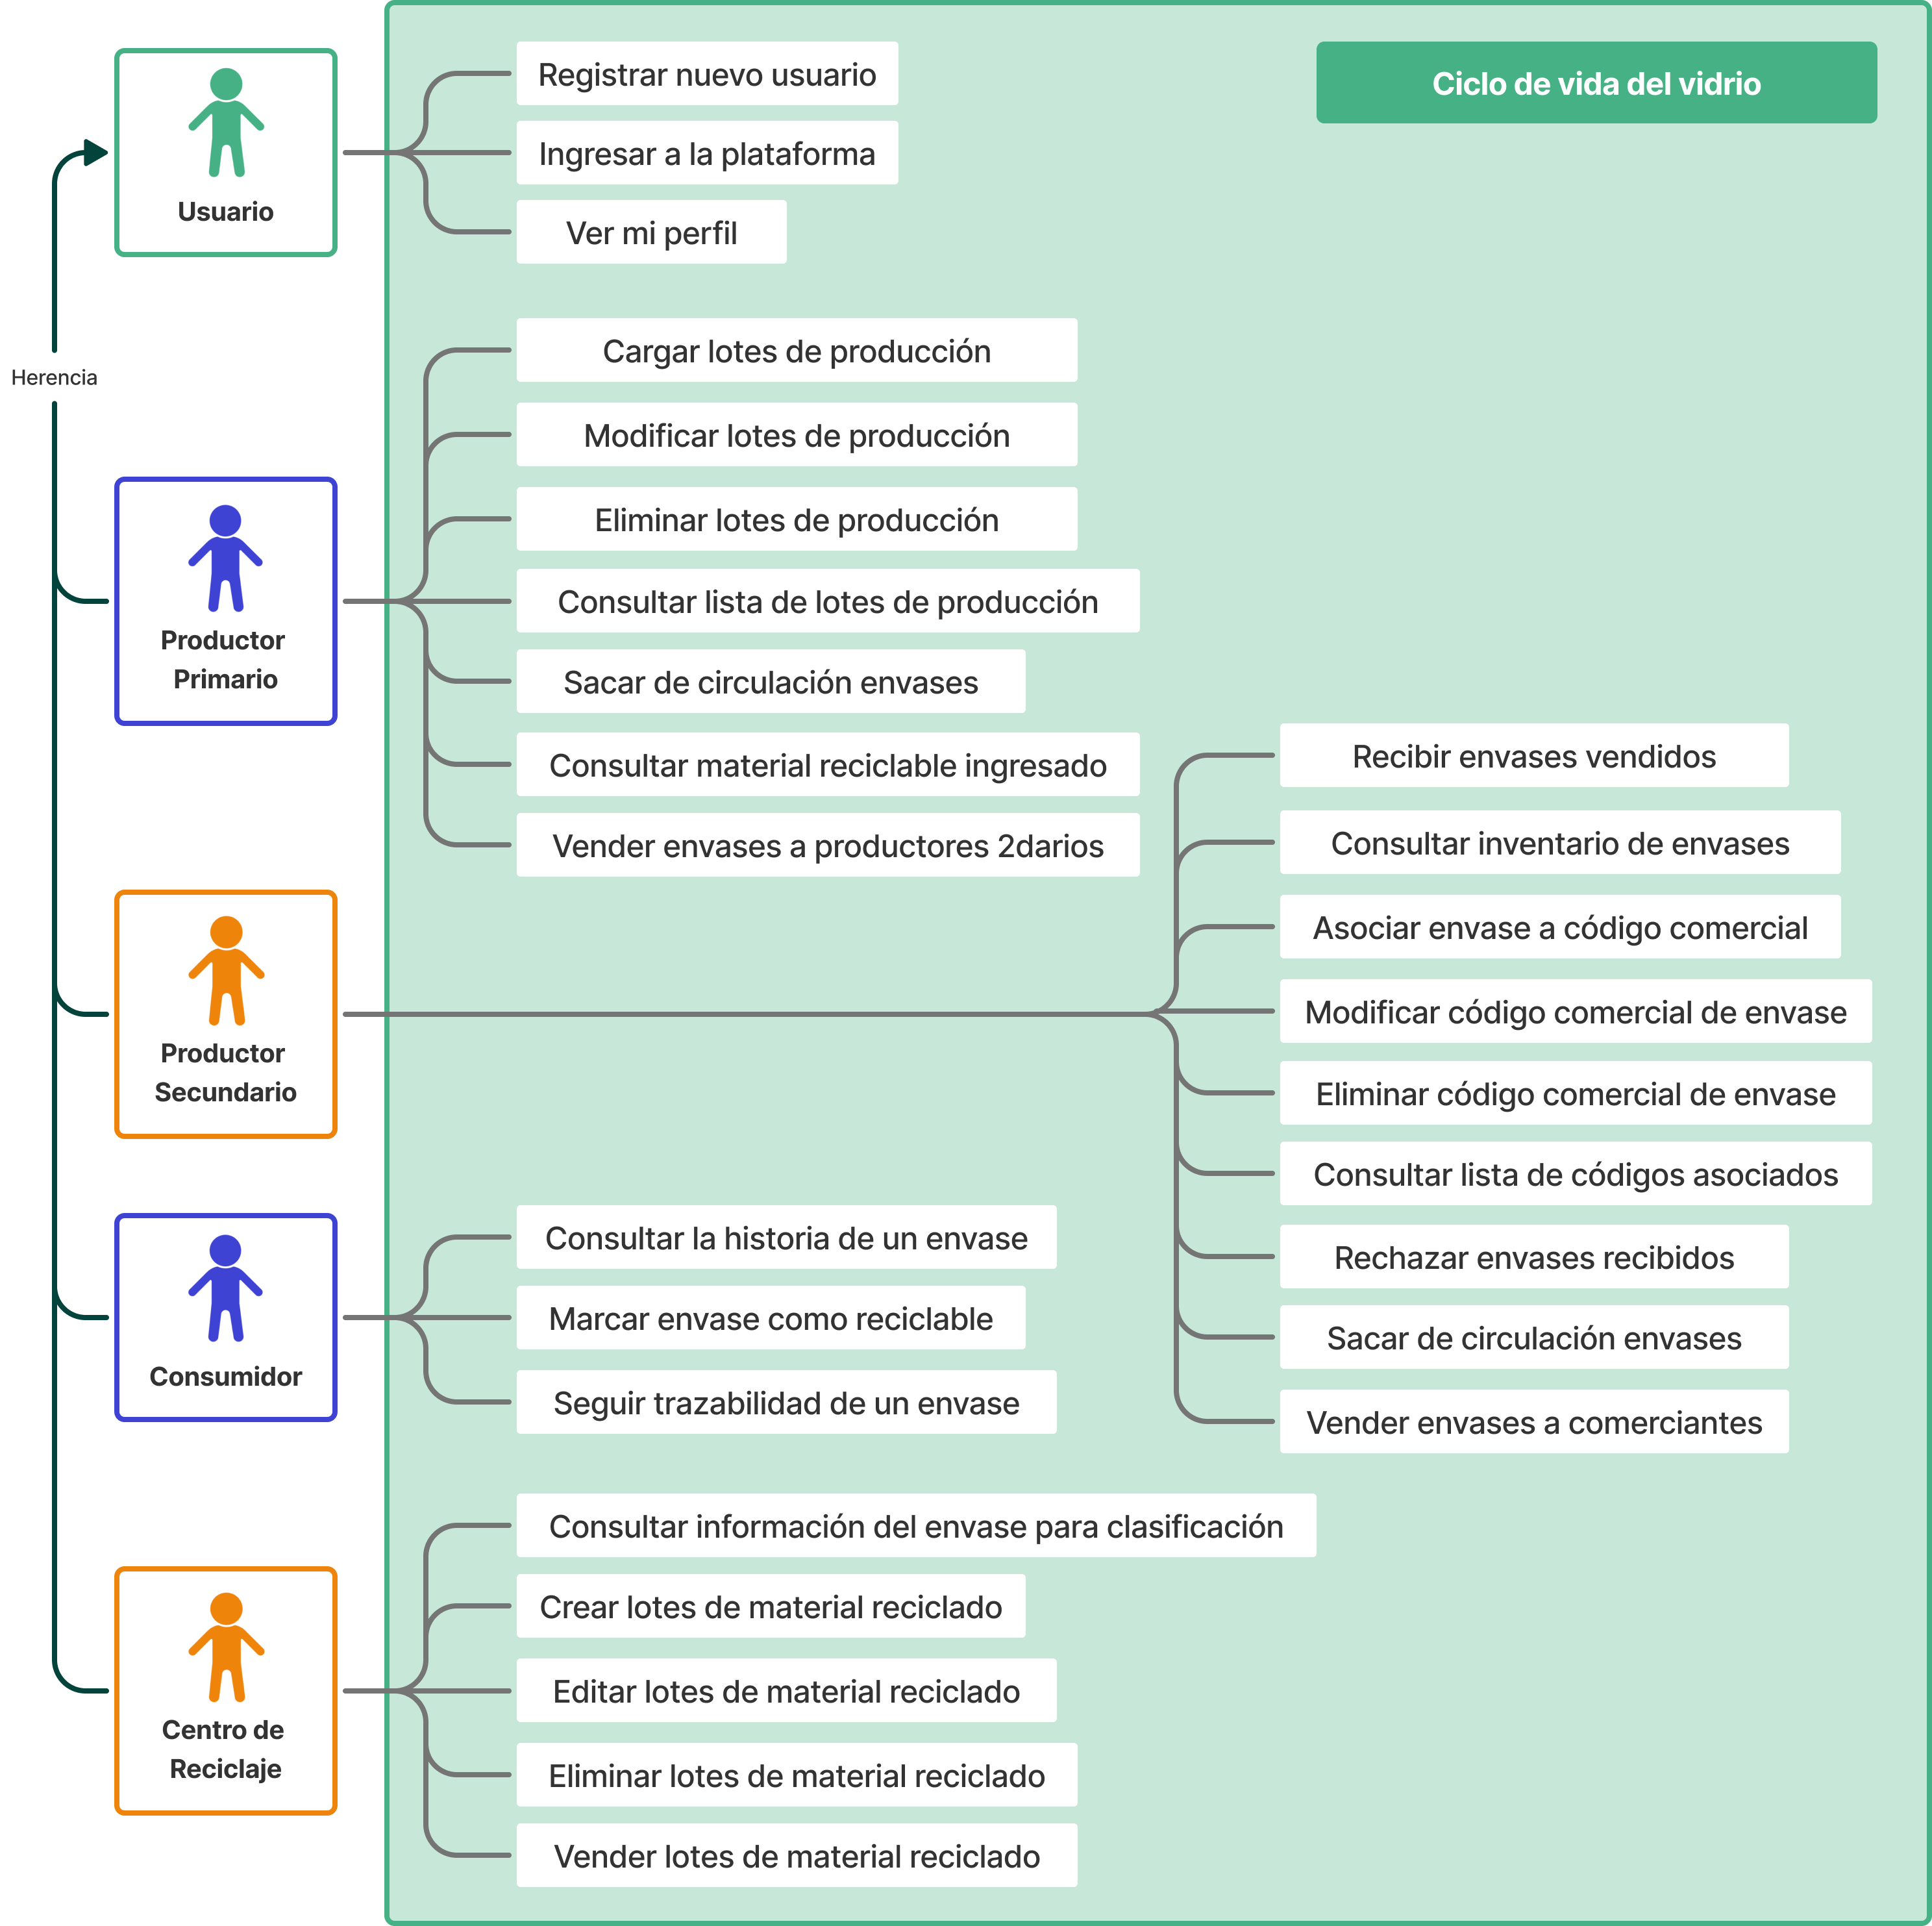
\includegraphics[width=0.8\textwidth]{Figures/use-case-diagram.png}
    \caption{Diagrama de Casos de Uso del sistema de trazabilidad de vidrio}
    \label{fig:use-case-diagram}
\end{figure}

El diagrama muestra que cada actor tiene un conjunto de casos de uso alineado con sus responsabilidades. Por ejemplo, el Productor Primario puede registrar un nuevo lote de envases producidos o registrar la venta de envases a un Productor Secundario, mientras que el Productor Secundario puede consultar la trazabilidad de origen de los envases recibidos y registrar su uso asociando los envases a un lote de producto final. Por otro lado, el Consumidor puede consultar el origen de un envase adquirido y el destino de un envase enviado a reciclaje, mientras que el Centro de Reciclaje puede recibir envases reciclables, consultar su composición de materiales y registrar su reciclaje. Los casos de uso de los diferentes actores se interrelacionan de manera cíclica, integrando la información de cada actor de la cadena en un único sistema de información interrelacionado que refleja el flujo de la economía circular de envases de vidrio. Por ejemplo, la acción "Vender envases a productores secundarios" del Productor Primario está ligada a los casos de uso del Productor Secundario, permitiendo rastrear el vidrio a lo largo de su ciclo de vida.

La lista de casos de uso sirve como punto de partida para la definición de los requerimientos funcionales y no funcionales del sistema, donde cada caso de uso se descompone en uno o más requerimientos específicos que describen las funcionalidades que el sistema debe implementar para cumplir con las expectativas de los actores.

\section{Definición de Requerimientos}
\label{sec:requirements-definition}

Después de identificar los casos de uso, se definen los requerimientos funcionales y no funcionales del sistema. Los requerimientos funcionales describen las funcionalidades específicas que el sistema debe ofrecer a los usuarios, mientras que los requerimientos no funcionales establecen las características de calidad que el sistema debe cumplir, tales como rendimiento, seguridad o usabilidad.

Los requerimientos se documentan de manera estructurada, asignando un identificador único a cada requerimiento para su seguimiento durante las etapas posteriores de diseño, implementación y pruebas del sistema. La descripción de cada requerimiento incluye su propósito, las condiciones bajo las cuales se cumple y las dependencias con otros requerimientos. Un ejemplo de requerimiento funcional es que "el sistema debe permitir al Productor de Vidrio registrar un nuevo lote de vidrio, especificando la cantidad y el tipo de vidrio", mientras que un requerimiento no funcional puede ser que "el sistema debe garantizar la seguridad de los datos del usuario mediante autenticación y autorización".

A partir de los casos de uso previamente identificados, se definieron 28 requerimientos funcionales y 6 requerimientos no funcionales para el sistema. Estos requerimientos se documentan en la etapa de modelado para su posterior seguimiento durante el desarrollo. Se establecen dependencias entre ellos, lo que permite identificar restricciones en el orden de implementación de las funcionalidades del sistema. Por ejemplo, el registro de un lote de vidrio (RF-006) es una dependencia para que dicho lote pueda ser recibido por un productor secundario para envasar productos (RF-016). La Tabla \ref{tab:functional-requirements} presenta los requerimientos funcionales, mientras que la Tabla \ref{tab:non-functional-requirements} muestra los requerimientos no funcionales definidos para el prototipo de trazabilidad de envases de vidrio basado en blockchain.

\begin{xltabular}{\textwidth}{@{} L{1.5cm} L{2.5cm} Y L{1.5cm} @{}}
	\caption{Requerimientos Funcionales del sistema de trazabilidad de envases de vidrio}
	\label{tab:functional-requirements}\\
	\toprule
	ID & Título & Descripción & Deps \\
	\midrule
\endfirsthead

\toprule
ID & Título & Descripción & Deps \\
\midrule
\endhead

\midrule
\multicolumn{4}{r}{\footnotesize Continúa en la siguiente página}
\\\bottomrule
\endfoot

\bottomrule
\endlastfoot
	RF-001 & Registrar usuarios & El sistema debe permitir registrar usuarios mediante correo electrónico u otro medio con diferentes roles para hacer uso de las distintas partes del sistema. Los roles disponibles en esta primera etapa son: Productor Primario, Productor Secundario, Consumidor y Reciclador. & - \\
	RF-002 & Ingresar a la plataforma & Todos los usuarios deben poder ingresar a la plataforma con su correo electrónico registrado mediante algún método de autenticación con contraseña, OTP, 3rd party, etc. & RF-001 \\
	RF-003 & Mantener sesión de usuario & Cada cuenta de usuarios debe poder mantener abiertas múltiples sesiones en simultaneo. El usuario debe cerrar una sesión individual en cualquier dispositivo. La sesión debe mantenerse abierta en el dispositivo a lo largo del tiempo a pesar de que se cierre el navegador o aplicación. & RF-002 \\
	RF-004 & Validar Autorización & Cada rol de usuario debe tener ciertos permisos y un usuario con un rol dado no debe poder realizar acciones que requieran un permiso del que no goza. Detalle:\n Productor: CRUD productos.\n Comerciante: RU productos (transferencia de propiedad de productos)\n Consumidor: R productos (consultar composición de productos)\n Reciclador: R productos, CRUD lotes de reciclaje. \n Invitados (sin autenticación): permiso de lectura en todo el sistema (R productos, R lotes de reciclaje). & RF-002 \\
	RF-005 & Ver mi perfil de usuario & Cada usuario debe poder consultar la información personal asociada a su cuenta y modificar algunos datos: Email, Nombre Empresa/persona (modificable), Responsable (modificable), Nro teléfono (modificable), Dirección pública blockchain. & RF-002 \\
	RF-006 & Cargar lotes de producción & El productor puede cargar lotes de producción de envases de vidrio incluyendo la siguiente información: Cantidad de envases, Peso por envase, Color, Composición, Espesor, entre otras. & RF-004 \\
	RF-007 & Editar lotes de producción & El productor puede editar la información de producción en caso de equivocación hasta antes de comercializar el lote. & RF-006 \\
	RF-008 &Eliminar lotes de producción &El productor puede eliminar un lote en caso de equivocación hasta antes de comercializar el lote. & RF-006 \\
	RF-009 & Consultar historial de producción & El productor puede consultar información histórica de todos los lotes que ha creado con sus detalles y puede consultar su trazabilidad posterior. & RF-006 \\
	RF-010 & Consultar material reciclable ingresado & El productor puede ver la lista de los lotes o conjuntos de materiales reciclables que volvieron a ingresar a su fábrica (como compra a la recicladora o devoluciones desde bodegas). & RF-006, RF-018, RF-025 \\
	RF-011 & Sacar de circulación envases & El productor puede marcar grupos de botellas de un lote como fuera de circulación o enviado a reciclar (en caso de rotura, falla o desaparición). & RF-006 \\
	RF-012 & Vender envases a productores secundarios & El productor puede marcar cierta cantidad de envases del lote como vendidos a un productor secundario específico. Los envases dejan de ser propiedad del productor y ya no puede modificarlos ni revenderlos. & RF-006 \\
	RF-013 & Asociar envase a código comercial & El productor secundario puede asociar un código de barras (u otro tipo de código visible en la etiqueta impresa de su producto, como QR) a conjuntos de botellas compradas. EL CÓDIGO DEBE GARANTIZAR UNICIDAD. & RF-012 \\
	RF-014 & Modificar código comercial & El productor secundario puede editar la información de códigos asociados a envases hasta antes de vender el producto. & RF-013 \\
	RF-015 & Eliminar código comercial & El productor secundario puede eliminar códigos asociados a envases hasta antes de vender el producto. & RF-013 \\
	RF-016 & Consultar inventario de envases nuevos & El productor secundario puede ver la lista de conjuntos de envases que ha comprado pero aún no ha utilizado (no han sido asociados a ningún producto propio ni código). El productor puede confirmar conformidad o rechazar la compra. & RF-012 \\
	RF-017 & Rechazar envases recibidos & El productor secundario puede desconocer la transacción de transferencia de envases desde el productor en caso de no reconocer la compra o realizar una devolución por algún tipo de error. & RF-012 \\
	RF-018 & Sacar de circulación envases & El productor secundario puede devolver botellas en caso de no conformidad, fallas de fábrica o rotura. Estos envases pueden transferirse al productor como material reciclable o descartarse. & RF-012 \\
	RF-019 & Consultar historial de producción & El productor secundario puede consultar el historial de sus productos embotellados o botellas utilizadas. A su vez puede consultar su trazabilidad posterior a la comercialización. & RF-013 \\
	RF-020 & Vender envases a comerciantes & El productor secundario puede marcar sus productos embotellados como vendidos al comerciante. & RF-013 \\
	RF-021 & Consultar la historia de un envase & Mediante el código asociado a la botella, el ciudadano debe poder consultar el origen, composición y trazabilidad histórica de envase cualesquiera. & RF-013 \\
	RF-022 & Marcar envase como reciclable & El ciudadano puede registrar un envase como ingresado al sistema de reciclaje escaneando su código. & RF-013 \\
	RF-023 & Dar seguimiento a envases & El ciudadano puede hacer seguimiento del destino y trazabilidad hasta la disposición final de todos los envases que ingresó al sistema de reciclaje. & RF-022 \\
	RF-024 & Consultar información del envase para clasificación & El reciclador clasificador puede escanear el código de la botella y obtener información relevante sobre su composición para su correcta clasificación. & RF-013 \\
	RF-025 & Crear lotes de material reciclado & El reciclador puede crear lotes de material reciclado a partir de un conjunto de envases reciclables recibidos de los ciudadanos. Cada lote tiene los siguientes atributos: Peso, Dimensión (si aplica), Material, Composición. & RF-022 \\
	RF-026 & Editar lote de material reciclado & El reciclador puede editar la información de un lote en caso de equivocación hasta antes de su comercialización. & RF-025 \\
	RF-027 & Eliminar lote de material reciclado & El reciclador puede eliminar un lote en caso de equivocación hasta antes de su comercialización. & RF-025 \\
	RF-028 & Vender lote de material reciclado & El reciclador puede marcar un lote de material reciclable como vendido a un productor y debe especificar el comprador. Se asume en este caso que el material fue efectivamente reciclado, finalizando la trazabilidad. & RF-025 \\
\end{xltabular}

\begin{xltabular}{\textwidth}{@{} L{1.5cm} L{2.5cm} Y @{}}
	\caption{Requerimientos No Funcionales del sistema de trazabilidad de envases de vidrio}
	\label{tab:non-functional-requirements}\\
	\toprule
	ID & Título & Descripción \\
	\midrule
\endfirsthead

\toprule
ID & Título & Descripción \\
\midrule
\endhead

\midrule
\multicolumn{4}{r}{\footnotesize Continúa en la siguiente página}
\\\bottomrule
\endfoot

\bottomrule
\endlastfoot
RNF-01 & Transparencia & La trazabilidad de un producto debe ser libremente accesible por cualquier usuario autenticado del sistema en todo momento. \\
RNF-02 & Disponibilidad & El sistema debe estar disponible para su uso 24/7 \\
RNF-03 & Escalabilidad & El sistema debe soportar un nro creciente de transacciones \\
RNF-04 & Mantenibilidad & El sistema debe poder ser mantenible por otros desarrolladores de la industria actual en un futuro \\
RNF-05 & Interoperabilidad & El sistema debe ser integrable con otros múltiples sistemas de stock y gestión de terceros preexistentes \\
RNF-06 & Integridad & Los datos de trazabilidad no deben poder ser alterados luego de cargados sin dejar registro público de la modificación \\
\end{xltabular}

La lista de requerimientos funcionales y no funcionales sirve como base para la siguiente fase de modelado, en la que se definirán las historias de usuario y se planificará el desarrollo del sistema. A su vez, la lista de requerimientos se utilizará posteriormente en la validación y verificación del sistema, asegurando que todas las funcionalidades implementadas cumplan con las expectativas y necesidades de los usuarios.

\section{Historias de Usuario y Planificación}
\label{sec:user-stories}

A partir de la definición de los requerimientos funcionales y no funcionales del sistema, se procede a la creación de las historias de usuario. Las historias de usuario permiten documentar las funcionalidades del sistema desde la perspectiva de sus actores, utilizando un formato estandarizado que describe el rol, la acción deseada y el beneficio esperado: "Como [rol], quiero [acción], para [beneficio]". Por ejemplo, "Como Productor Primario,  
quiero poder editar la información de un lote de envases antes de su comercialización, para poder corregir cualquier error en los datos de producción y asegurar la precisión en el registro". Esta forma de documentar requerimientos facilita la priorización de funcionalidades y la comprensión de las necesidades desde un enfoque centrado en el usuario a la hora de desarrollar el sistema.

Cada historia de usuario se complementa con criterios de aceptación que establecen las condiciones necesarias para su validación, vinculándose directamente con uno o más requerimientos previamente definidos. Esta trazabilidad entre los requerimientos y las historias de usuario es un mecanismo de control que guía el proceso de desarrollo y asegura que la implementación cumpla con las expectativas planteadas. En el contexto del modelo en V, las historias de usuario establecen la base para la fase de pruebas de aceptación, garantizando que el sistema final se alinee con los objetivos del proyecto.

A continuación se presenta un ejemplo de historia de usuario con sus respectivos criterios de aceptación, que ilustra la relación entre las funcionalidades y las necesidades de los actores.

\begin{center}
\fbox{
  \begin{minipage}{0.95\linewidth}
    \textbf{Historia de Usuario:} Consultar historial de producción de lotes de envases de vidrio \\
    \textbf{Como} productor, \\
    \textbf{Quiero} poder consultar el historial de todos los lotes de producción con sus detalles y trazabilidad, \\
    \textbf{Para} poder revisar la información de producción y rastrear cada lote en su ciclo de vida.
    
    \vspace{0.5cm}
    
    \textbf{Criterios de Aceptación:}
    \begin{enumerate}
      \item \textbf{Visualización del historial de lotes:}
      \begin{itemize}
        \item El sistema debe mostrar una lista de todos los lotes creados por el productor con la siguiente información:
        \begin{itemize}
          \item \textbf{Código de lote}
          \item \textbf{Fecha de producción}
          \item Cantidad de envases
          \item Peso por envase
          \item Color
        \end{itemize}
      \end{itemize}
      
      \item \textbf{Acceso a detalles de cada lote:}
      \begin{itemize}
        \item Al seleccionar un lote específico, el sistema debe mostrar los detalles completos, incluyendo:
        \begin{itemize}
          \item Espesor
          \item \textbf{Fecha de producción}
          \item Observaciones adicionales
        \end{itemize}
      \end{itemize}
    \end{enumerate}
  \end{minipage}
}
\end{center}

En el presente trabajo, se definieron un total de 28 historias de usuario, donde cada historia de usuario se corresponde exactamente con un requerimiento funcional del sistema. Los requerimientos no funcionales se abordan de manera transversal, asegurando que aspectos como el rendimiento, la seguridad y la usabilidad sean considerados en el diseño e implementación del sistema.

Para la gestión del proceso de desarrollo, las historias de usuario se registraron en la herramienta Jira, un software para gestión de proyectos de desarrollo de software compatible con la metodología Kanban. Esta herramienta permite gestionar el flujo de trabajo, asignar tareas a los miembros del equipo y realizar un seguimiento del progreso durante el desarrollo. Como parte del proceso de planificación, se estimó el esfuerzo necesario para realizar cada tarea y se registró en la herramienta Jira junto con la tarea. La estimación del esfuerzo consideró la complejidad técnica, el tiempo requerido proyectado para implementarlo y las interdependencias entre las funcionalidades, lo que permitió una planificación objetiva del desarrollo.

La planificación del proyecto se realizó mediante un diagrama de Gantt. Un diagrama de Gantt es una herramienta visual que muestra la secuencia de las tareas, sus dependencias y los plazos de implementación estimados. Este diagrama permite visualizar el cronograma del proyecto, facilitando la identificación de hitos y la gestión de recursos. En este caso, se utilizó para planificar las historias de usuario y su implementación en iteraciones o sprints, asegurando que todas las funcionalidades necesarias sean contempladas y ejecutadas de manera ordenada según sus dependencias.

En la Figura \ref{fig:jira-board}, se muestra una captura del tablero utilizado para el seguimiento del progreso de cada historia de usuario en la plataforma Jira, mientras que la Figura \ref{fig:gantt-chart} presenta el diagrama de Gantt que ilustra la secuencia de las tareas, sus dependencias y los plazos de implementación estimados. Con la planificación armada, se estimó que el desarrollo del sistema tendría una duración de 6 semanas, con un total de 28 historias de usuario a implementar. Esta estimación de tiempo corresponde exclusivamente al tiempo de codificación de funcionalidades del prototipo, ya que, posterior a la etapa de generación de código, se procede a la fase codificación y ejecución de pruebas automatizadas y validación manual del sistema, donde es posible a su vez que se deban realizar ajustes o correcciones de programación en función de los resultados obtenidos.

\begin{figure}[!htpb]
  \centering
  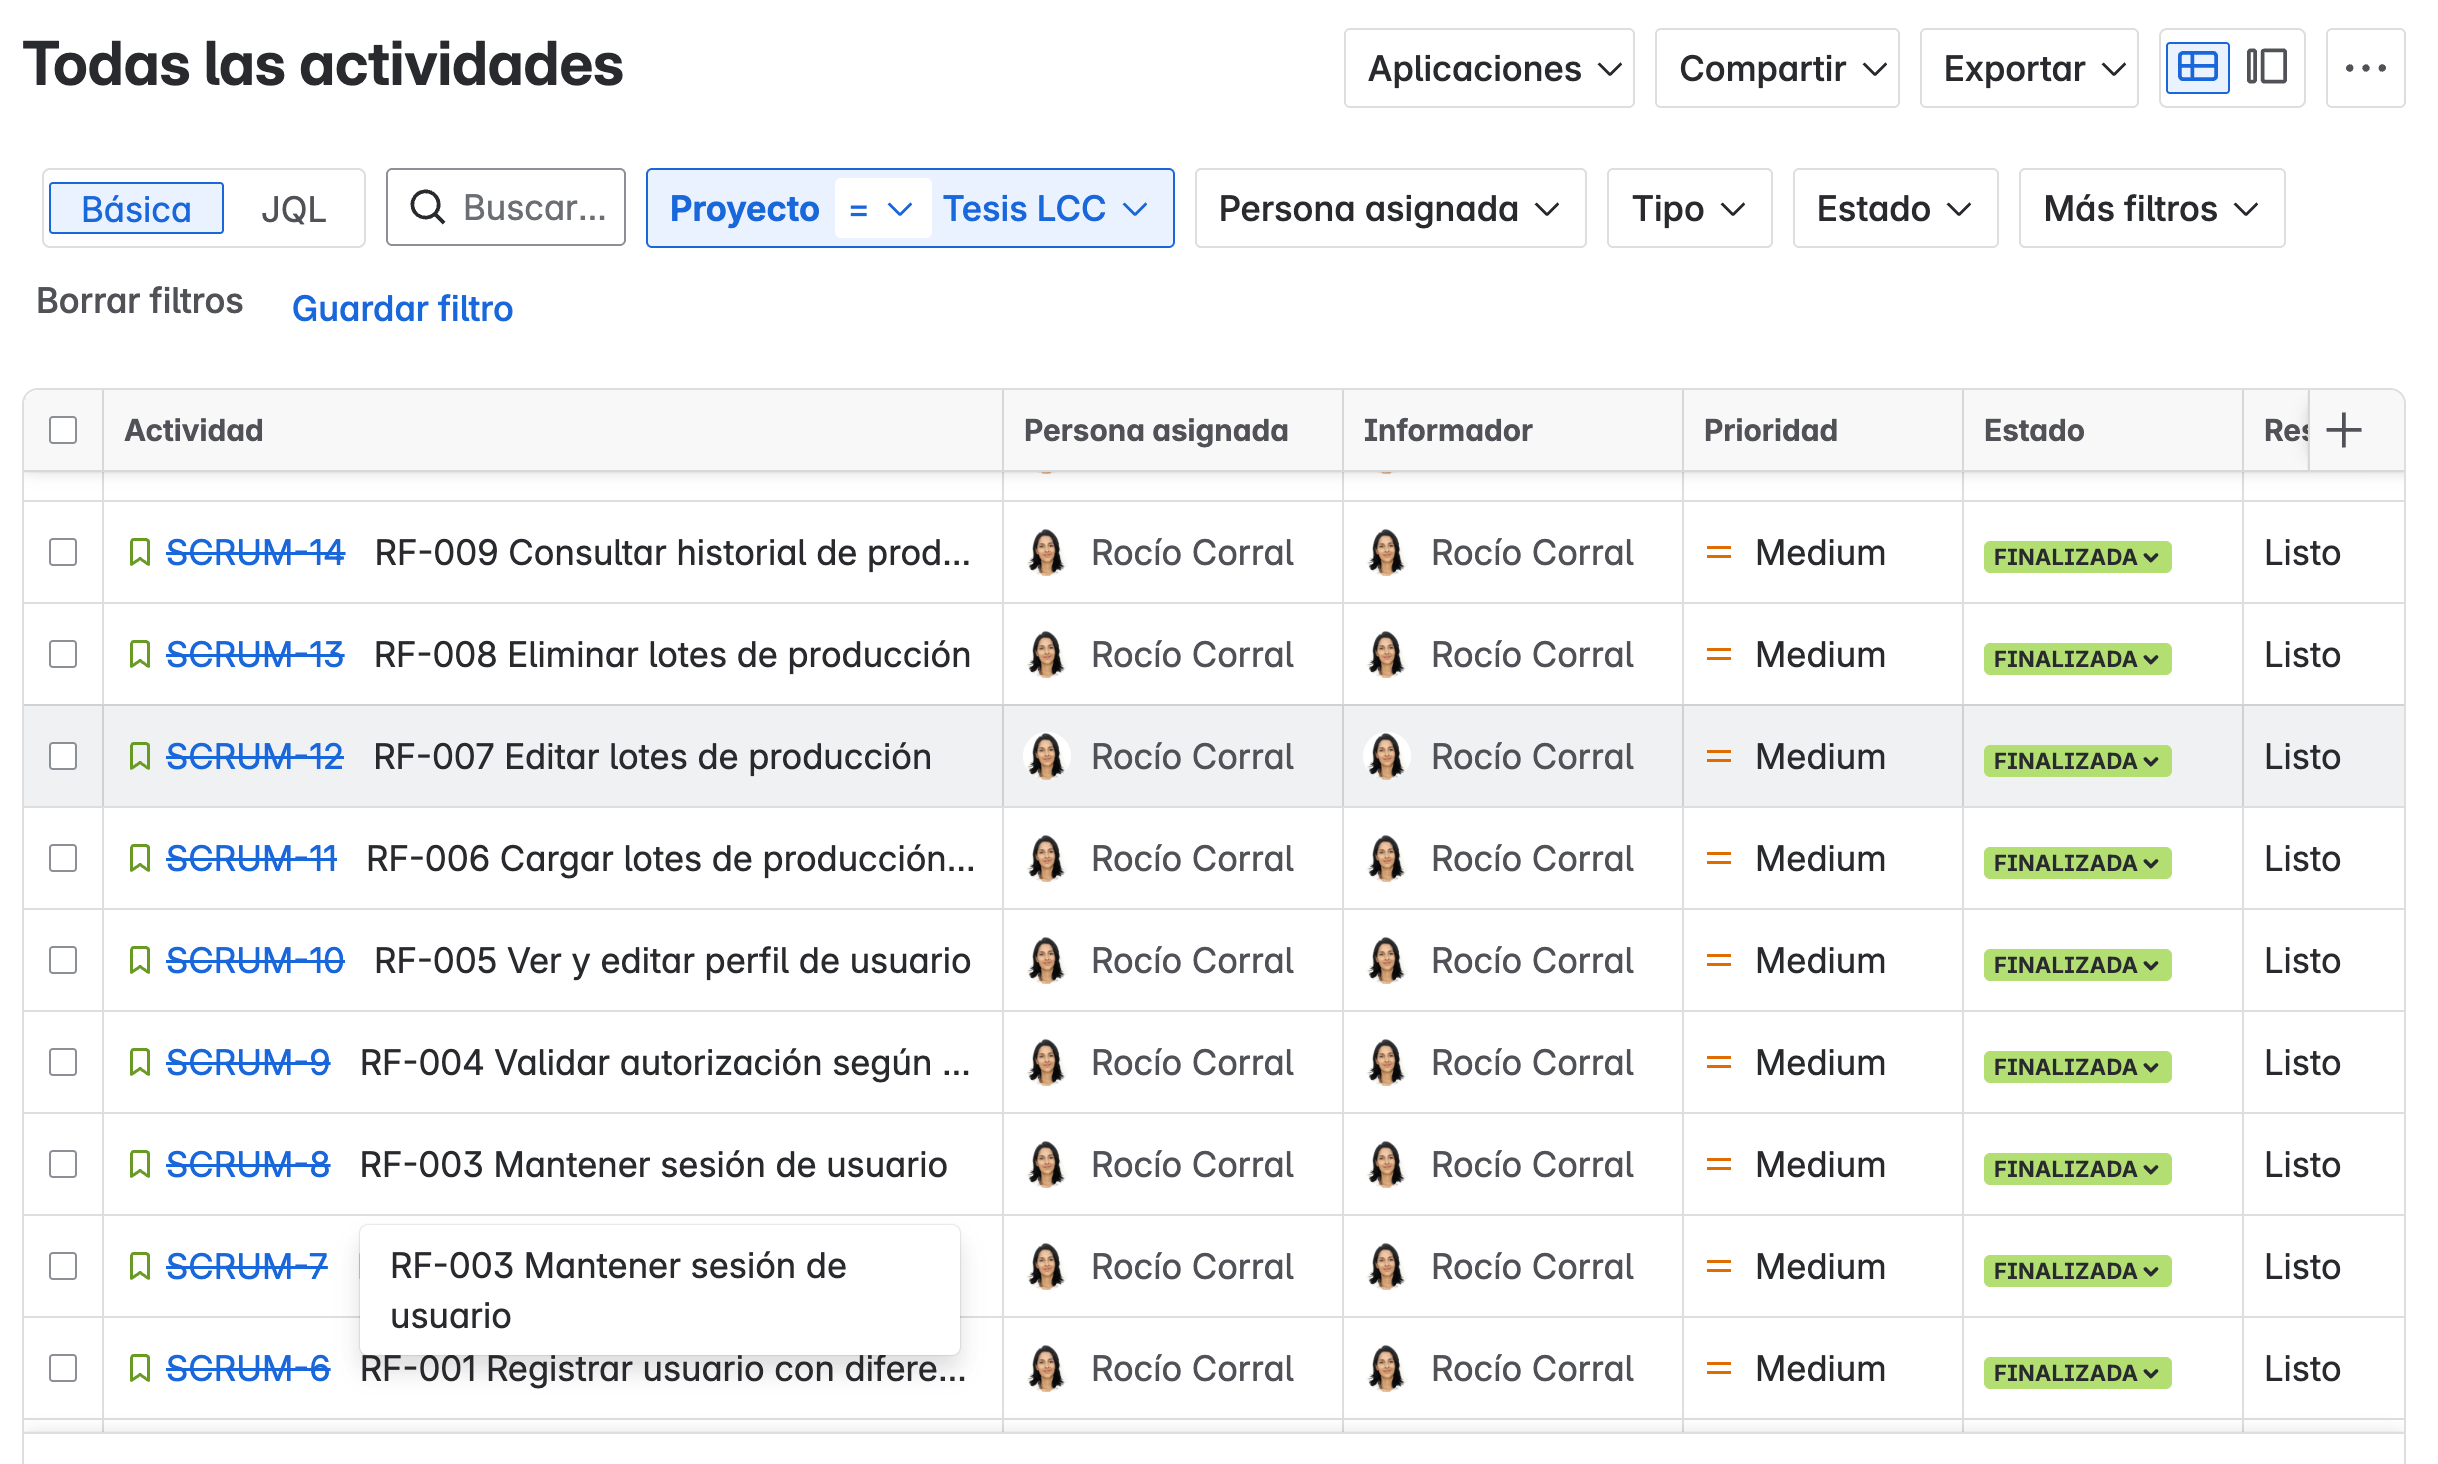
\includegraphics[width=0.8\textwidth]{Figures/jira-board.png}
  \caption{Tablero de Jira para la gestión de historias de usuario}
  \label{fig:jira-board}
\end{figure}

% TODO: resolve the content and format of these images. 

\begin{figure}[!htpb]
  \centering
  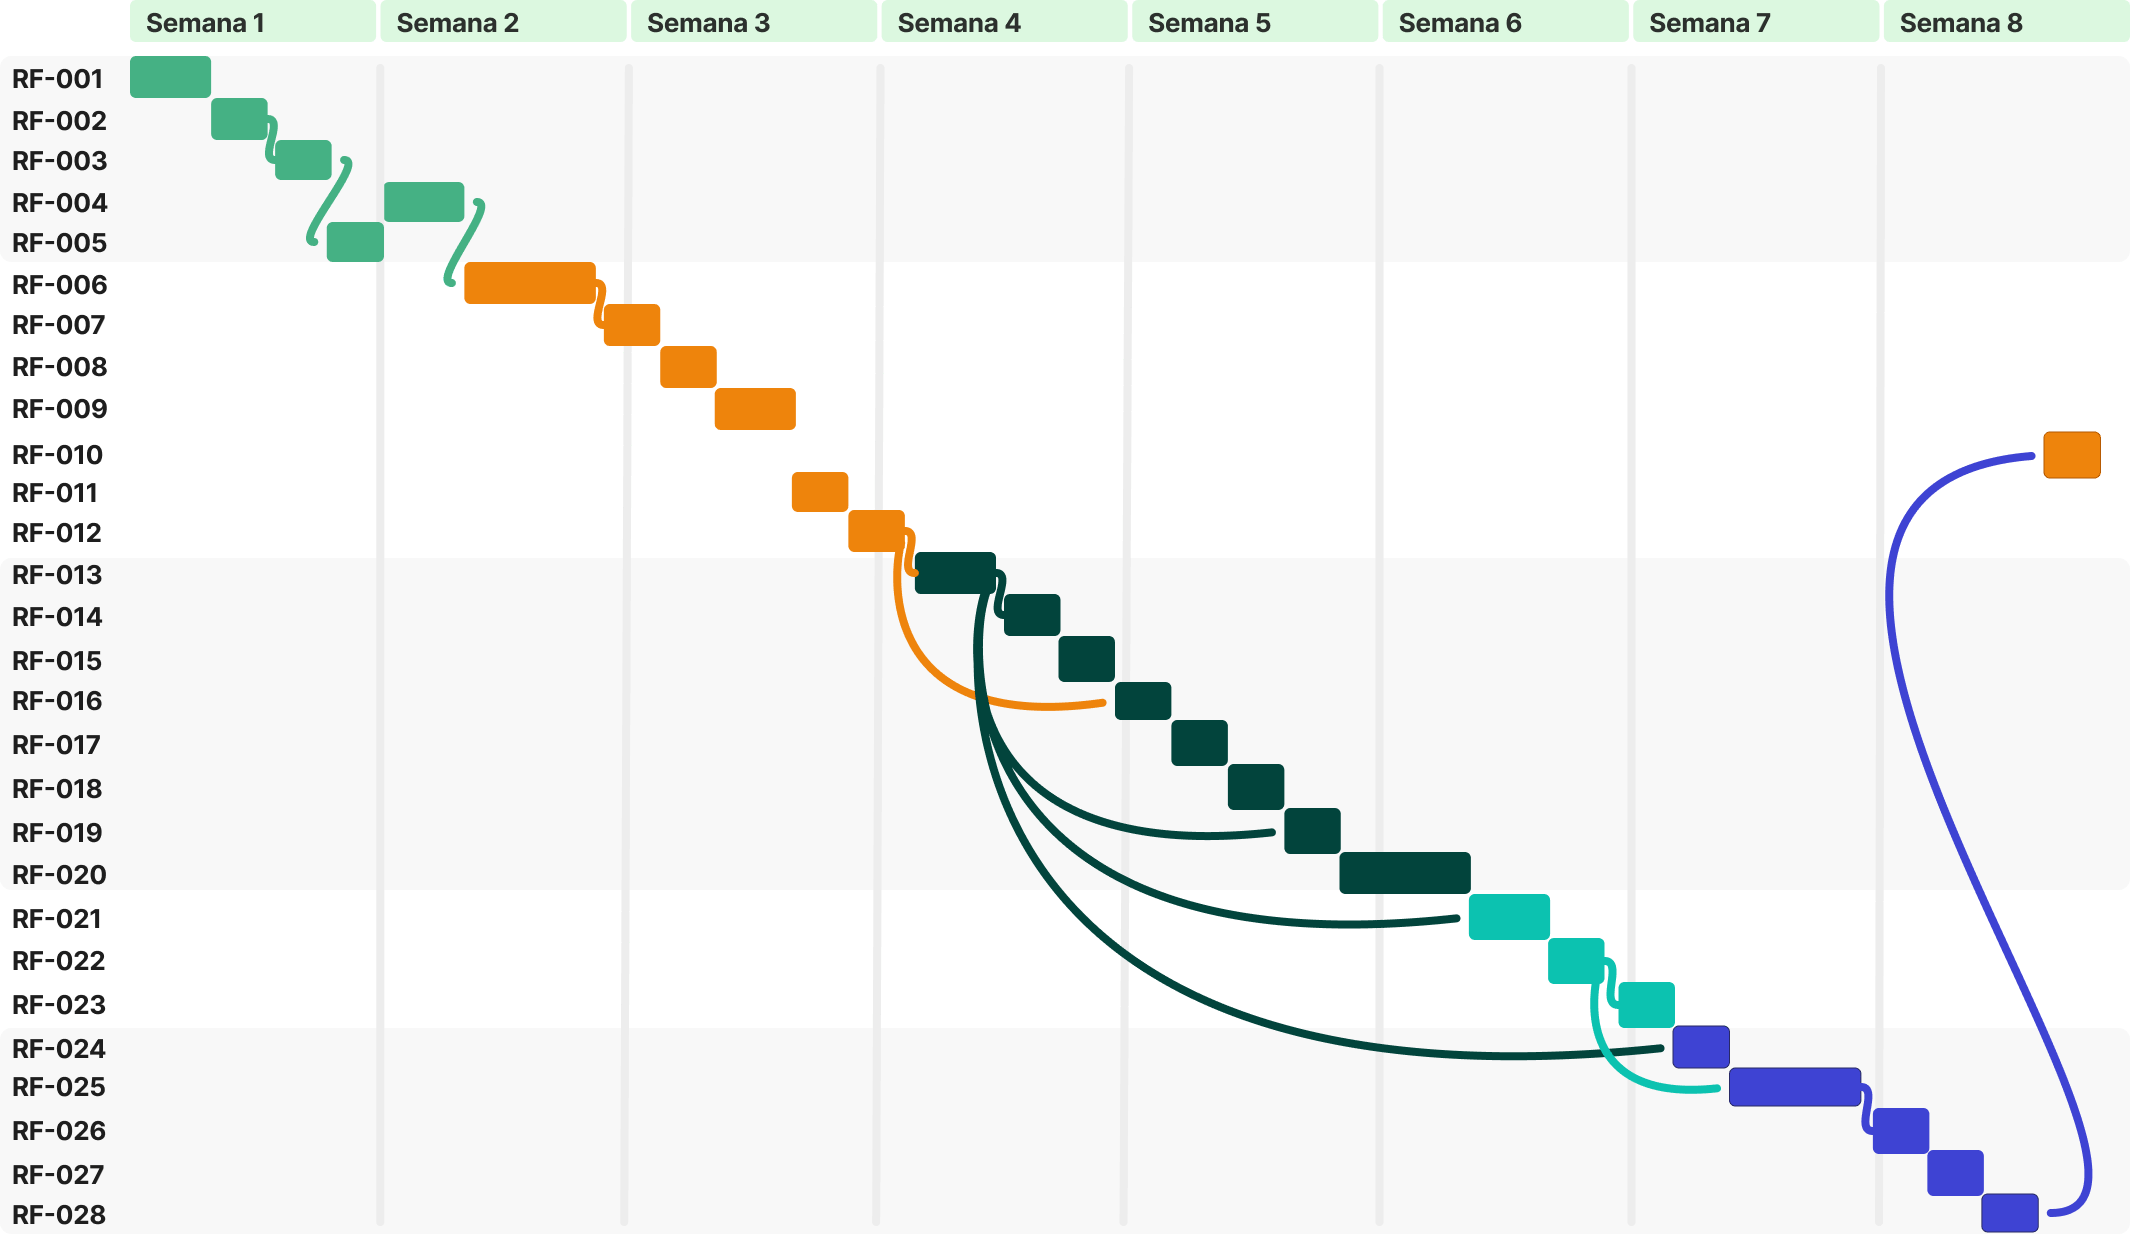
\includegraphics[width=0.8\textwidth]{Figures/gantt-chart.png}
  \caption{Diagrama de Gantt para la planificación del proyecto}
  \label{fig:gantt-chart}
\end{figure}

Concluidas las fases de modelado de requerimientos y planificación, se establece la base para la siguiente etapa del proceso. El conjunto de requerimientos, casos de uso y la planificación detallada con las historias de usuario constituyen la referencia que guiará las fases de diseño, implementación y pruebas del sistema. En el próximo capítulo, se abordará el diseño de la arquitectura y los componentes del sistema, donde se definirán las soluciones tecnológicas y la estructura del software que implementará los requerimientos establecidos.

\chapter[Diseño de solución]{Diseño de Solución}
\label{cp:design}

\parindent0pt

En la fase de modelado de requerimientos se definieron las bases del sistema, estableciendo sus funcionalidades y características que el prototipo debe cumplir. A partir de estas bases, es posible proceder a la etapa de diseño de solución, que es una transición entre la especificación de lo que el sistema debe hacer y el cómo se construirá, transformando los requerimientos abstractos en una arquitectura concreta y un plan de implementación. El diseño permite obtener una visión integral del sistema antes de iniciar la implementación, lo que facilita la identificación de dependencias e interfaces y asegura que todos los componentes y módulos interactúen de manera coherente. Este proceso de planificación anticipada reduce la probabilidad de encontrar inconsistencias o funcionalidades indefinidas durante las fases de desarrollo y pruebas.

El diseño de la solución, en el marco del modelo en V, se aborda en dos etapas: primero se realiza el diseño de arquitectura y luego el diseño de componentes. Cada una de estas etapas se enfoca en un nivel de abstracción distinto del sistema. El diseño de arquitectura comprende la definición de la estructura general del sistema a través de módulos, mientras que el diseño de componentes se ocupa de los detalles internos de cada módulo.

En la primera etapa, diseño de arquitectura, el sistema se divide en subsistemas o módulos lógicos y se definen sus interacciones, las responsabilidades de cada uno y las tecnologías subyacentes. Este enfoque permite establecer las bases del sistema, abarcando tanto los requerimientos funcionales como los no funcionales. Las decisiones de diseño tomadas en esta etapa se validan posteriormente mediante pruebas de sistema, las cuales se encargan de verificar que todos los módulos trabajen conjuntamente y que el sistema de forma integral satisfaga los requerimientos especificados.

Por otro lado, la segunda etapa es el diseño de componentes, donde se profundiza en los detalles de la arquitectura interna de cada módulo. Esto incluye la especificación de clases, interfaces, flujos de datos y la organización de la lógica de negocio. Los requerimientos funcionales, guiados por las historias de usuario, se traducen en documentos de arquitectura de \gls{software} específicos que posteriormente se implementan en la fase de codificación. Las decisiones de diseño tomadas en esta etapa se verifican a través de las pruebas de integración, que aseguran que los componentes individuales interactúen de forma correcta entre sí.

Los requerimientos funcionales, definidos en el capítulo anterior, son el fundamento para el diseño de la solución y se utilizan en esta etapa a través de las historias de usuario, que guían el diseño de los módulos y componentes. De manera complementaria, los requerimientos no funcionales también se contemplan en la fase de diseño, particularmente en el diseño de arquitectura, donde se establecen las bases para garantizar atributos como la seguridad, el rendimiento y la escalabilidad, incluso si no están directamente asociados a una historia de usuario.

A continuación, se explicará cada una de las etapas del diseño de solución, comenzando con el diseño de arquitectura en la Sección \ref{sec:module-design}, para luego avanzar con el diseño de componentes en la Sección \ref{sec:components-design}.

\section{Diseño de arquitectura}
\label{sec:module-design}

La fase de diseño de arquitectura representa el primer paso en la traducción de los requerimientos del sistema hacia un sistema de \gls{software} funcional. El diseño permite una visión global de la solución, asegurando que todos los componentes y módulos trabajen juntos de manera coherente previo a la implementación. A partir de los requerimientos previamente definidos, se establece un marco de trabajo de alto nivel que estructura la solución en componentes lógicos, delineando sus responsabilidades, las interacciones entre ellos y las tecnologías que los soportan. La salida de esta etapa es la arquitectura del sistema, la cual servirá de base para las decisiones de diseño a un nivel más granular. En el contexto del modelo en V, las decisiones tomadas en esta etapa se validan en la fase de pruebas de sistema, donde se verifica que la arquitectura en su conjunto cumple con las especificaciones definidas en los requerimientos funcionales y no funcionales del sistema.

\begin{figure}[!tb]
    \centering
    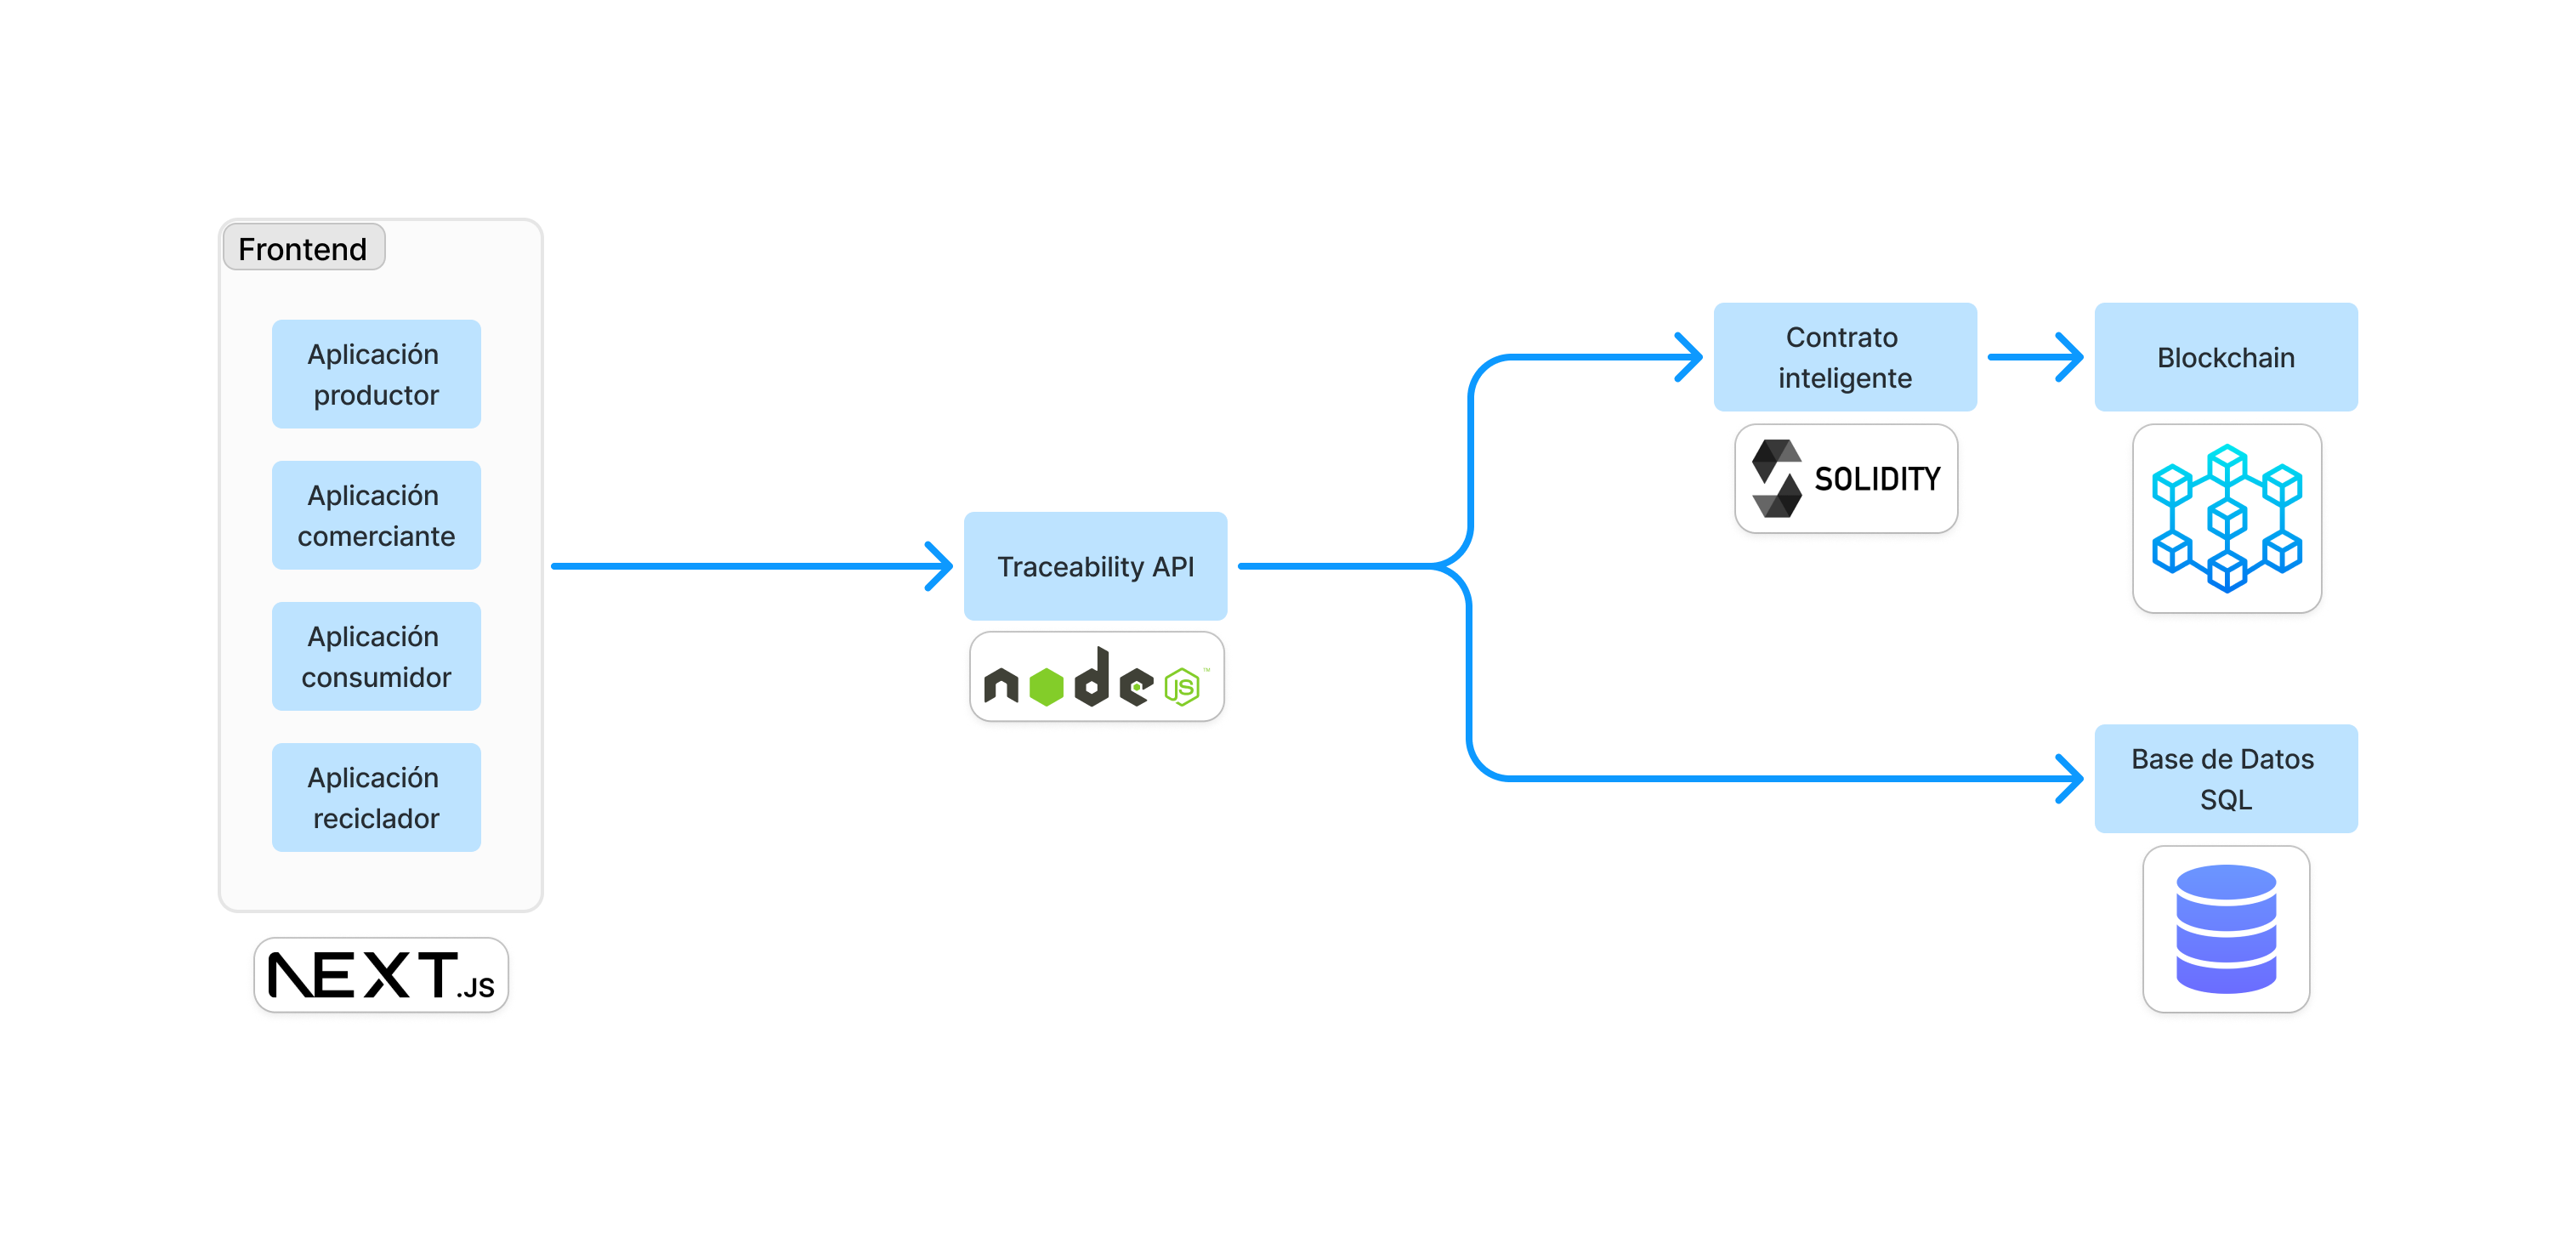
\includegraphics[width=\linewidth]{Figures/software-architecture.png}
    \caption{Arquitectura de módulos del sistema de trazabilidad de envases de vidrio basado en \textit{blockchain}}
    \label{fig:software-architecture}
\end{figure}

Para el prototipo tecnológico de trazabilidad de vidrio basado en \textit{blockchain}, la arquitectura del sistema se concibió siguiendo un enfoque de tres capas lógicas para asegurar una clara separación de responsabilidades y modularidad. Este patrón, común en el desarrollo de aplicaciones web, permite que cada capa se desarrolle, mantenga y escale de forma independiente. En la Figura \ref{fig:software-architecture} se ilustra el diseño de la arquitectura de módulos del sistema elaborado siguiendo este enfoque. La arquitectura se compone de la capa de presentación (\textit{\gls{frontend}}), la capa de lógica de negocio (\textit{\gls{backend}}) y la capa de datos (\textit{\gls{blockchain}} y \gls{basededatos} relacional). La comunicación entre estas capas se define a través de interfaces estandarizadas, lo que promueve una baja dependencia y puede facilitar futuras extensiones e integraciones, por ejemplo, con sistemas de gestión externos o con dispositivos \gls{iot} para automatizar la captura de datos en los procesos productivos.

A su vez, dentro de cada capa del sistema, es necesario definir un criterio para la delimitación de los módulos lógicos dentro de la misma capa. El criterio aplicado en este trabajo se basa en el principio de \textit{cohesión funcional}, el cual plantea agrupar las funcionalidades y responsabilidades del sistema a partir de cada rol de usuario identificado. Siguiendo este criterio, para este trabajo se decidió implementar un módulo específico para cada actor (productor primario, productor secundario, consumidor y centro de reciclaje), así como módulos compartidos para la lógica de negocio transversal, como la autenticación de usuarios o trazabilidad de envases de vidrio. Esta división de responsabilidades reduce el acoplamiento entre los módulos y simplifica el mantenimiento del sistema, en el caso de requerir cambios o actualizaciones en el futuro.

Luego de definir las capas que componen la arquitectura del sistema, es posible proceder a seleccionar las tecnologías más adecuadas para cada uno de los módulos definidos. La elección de tecnologías para cada capa busca satisfacer una serie de criterios técnicos y de negocio, incluyendo la compatibilidad con otras tecnologías, el rendimiento, la escalabilidad y el soporte de la comunidad. El diseño de la arquitectura tecnológica del sistema, incluyendo la definición de tecnologías, se realizó siguiendo un enfoque ``de adentro hacia afuera'', comenzando por la representación de los datos para luego diseñar su acceso (\textit{\gls{backend}}) y finalmente la forma en la cual los datos se muestran (\textit{\gls{frontend}}). Esta perspectiva se elige para priorizar la integridad y la persistencia de la información, que son pilares fundamentales de un sistema basado en \textit{blockchain}. Al abordar primero la capa de datos y la lógica de negocio (es decir, los \glspl{contratointeligente}), se puede garantizar que la estructura central del sistema sea robusta para disminuir el riesgo de inconsistencias en una etapa avanzada de la implementación. Este enfoque, en lugar de uno ``de afuera hacia adentro'' (del \textit{frontend} a los datos), asegura que la lógica de negocio sea el foco principal del diseño, permitiendo que la interfaz de usuario y otras capas de presentación se adapten a la funcionalidad central, y no al revés.

A continuación, se describen las tecnologías seleccionadas, los patrones de diseño aplicados y las decisiones arquitectónicas tomadas para cada capa del sistema. Comenzando por la capa de datos, se explicará la arquitectura desde adentro hacia afuera, siguiendo el flujo de datos desde su representación y almacenamiento hasta la presentación al usuario final.

\subsection{Capa de datos}

La capa de datos constituye el cimiento de todo sistema de software. Se encarga de la persistencia, gestión y recuperación de toda la información del sistema. Las bases de datos relacionales son el tipo de \gls{basededatos} más utilizado actualmente para gestionar información estructurada. Los datos se organizan en tablas, con filas y columnas, y se pueden establecer relaciones entre las distintas tablas mediante claves únicas. Cada columna tiene un nombre y un tipo de dato asociado, mientras que cada fila representa un registro único dentro de la tabla y su contenido debe cumplir con el tipo de dato definido para cada columna. Por ejemplo, se podría definir una tabla ``Usuario'', para almacenar información sobre los usuarios del sistema, incluyendo columnas como ``nombre'' de tipo texto, ``correo electrónico'' de tipo texto y ``fecha de registro'' de tipo fecha, entre otras columnas. Cada fila en esta tabla representaría un usuario específico, con su nombre, correo electrónico y la fecha en que se registró en el sistema, entre otros datos. Las principales ventajas de las bases de datos relacionales radican en su capacidad para garantizar la uniformidad de los datos a través de esquemas definidos para cada tabla, así como la facilidad para realizar consultas y análisis complejos de manera eficiente. Sin embargo, su naturaleza centralizada las hace susceptibles a manipulaciones manuales difíciles de detectar, lo que justifica la necesidad de una tecnología complementaria, como la \textit{blockchain}, para registrar información que requiere garantías de integridad.

En este prototipo, la tecnología \textit{blockchain} resulta apropiada para registrar la información clave del sistema, que requiere inmutabilidad y transparencia para fomentar la confianza entre los distintos actores. Ejemplos de este tipo de información pueden ser la propiedad de los lotes de envases de vidrio o la \gls{trazabilidad} de los envases reciclados. Por este motivo, se tomó la decisión estratégica de combinar la \textit{blockchain} con una \gls{basededatos} relacional con el objetivo de resolver la necesidad de equilibrio entre la seguridad y la transparencia, con el rendimiento y la escalabilidad. La \textit{blockchain}, por su naturaleza, provee una fuente de información segura y transparente, pero puede presentar limitaciones en cuanto a la velocidad de las transacciones y el volumen de datos que permite consultar eficientemente. Para abordar estas limitaciones, es que se decidió utilizar la \textit{blockchain} como base de datos principal del sistema, mientras que se decidió utilizar una base de datos relacional complementaria para almacenar datos auxiliares e indexar los datos de acceso frecuente, como los perfiles de usuario, los metadatos de los lotes (\textit{id}, propietario, estado, etc.) y otros datos de soporte que no requieren inmutabilidad. La relación entre ambas fuentes de datos se maneja mediante identificadores únicos que se almacenan en la \textit{blockchain}, sirviendo como una referencia a los datos detallados en la base de datos relacional. La capa \textit{\gls{backend}} es responsable de mantener la consistencia entre ambas fuentes de información (\textit{blockchain} y base de datos relacional) a la hora de persistir nueva información o actualizar información existente. Este enfoque híbrido permite proveer una recuperación de información ágil y una experiencia de usuario fluida sin poner en compromiso la integridad de los datos sensibles.

Luego de definir la estrategia de almacenamiento y gestión de datos, es posible proceder a seleccionar las tecnologías específicas que se utilizarán, tanto para la base de datos relacional como para la plataforma \textit{blockchain}, ya que existen múltiples opciones en el mercado.

En el caso de la base de datos relacional, se optó por el uso de MariaDB\footnote{\url{https://mariadb.org/documentation/}}, una base de datos de código abierto elegida por su sencillez y familiaridad, ya que el uso que se le dará en este trabajo es complementario y no hace falta utilizar una alternativa más compleja. MariaDB cuenta con un amplio soporte, librerías y documentación disponible para conectarse a ella de forma estandarizada desde cualquier lenguaje o \textit{framework} utilizado en la capa \textit{backend}.

Por otro lado, para la tecnología \textit{blockchain}, la elección de una plataforma adecuada puede determinar la complejidad y tiempo de implementación del sistema.  La tecnología \textit{blockchain} no se implementa desde cero, sino que se utilizan plataformas ya desarrolladas y probadas que ofrecen características y funcionalidades específicas. Estas plataformas, conocidas como protocolos \textit{blockchain}, varían en aspectos como su \gls{mecanismodeconsenso}, lenguaje de programación y comunidad de desarrolladores. Para este trabajo, se analizaron cinco de las plataformas líderes en la industria para su análisis y comparación: Hyperledger Fabric, Ethereum, Polkadot, VeChain y Cardano. Estas plataformas se seleccionaron por su relevancia y características técnicas, evaluando su idoneidad para el caso de uso específico de trazabilidad en la \gls{cadenadesuministro} del vidrio.

\textbf{Hyperledger Fabric}\footnote{\url{https://hlf.readthedocs.io/en/latest/}}
es una plataforma de código abierto diseñada para uso empresarial, que forma parte de la Fundación Linux \cite{androulaki2018hyperledger}. Se caracteriza por su arquitectura modular y configurable, ideal para una amplia gama de casos de uso en la industria. A diferencia de las redes públicas, es una plataforma permisionada, lo que significa que los participantes se conocen y confían entre sí. Admite \glspl{contratointeligente} en lenguajes de programación comunes como Java\footnote{\url{https://www.java.com/en/}} y Node.js\footnote{\url{https://nodejs.org/en}}, lo que reduce la curva de aprendizaje. Hyperledger no requiere una \gls{criptomoneda} nativa, lo que elimina ciertos riesgos de ataque y permite que la plataforma se implemente con costos operativos similares a los de cualquier otro sistema distribuido.

\textbf{Ethereum}\footnote{\url{https://ethereum.org/en/developers/docs/}}
es una plataforma de código abierto y pública que permite a los desarrolladores crear contratos inteligentes y aplicaciones descentralizadas (\gls{dapps}). Se considera una computadora mundial descentralizada, alimentada por su \gls{criptomoneda} nativa, Ether. Ethereum fue pionera en la creación de contratos inteligentes y ha mantenido un liderazgo en la industria desde su lanzamiento en 2015. Los contratos se escriben en Solidity\footnote{\url{https://www.soliditylang.org/}}, un lenguaje de programación de dominio específico que se ejecuta en la red de Ethereum. Este lenguaje de programación en la actualidad es el más utilizado para el desarrollo de contratos inteligentes. Aunque Ethereum se lanzó con un protocolo de consenso de Prueba de Trabajo (\acrshort{pow}), la plataforma ha migrado a la Prueba de Participación (\acrshort{pos}) para mejorar su eficiencia energética y escalabilidad.

\textbf{Polkadot}\footnote{\url{https://docs.polkadot.com/}}
es una plataforma de código abierto que busca facilitar la interoperabilidad entre diferentes \textit{blockchains}. Su objetivo es crear una red escalable y segura que pueda soportar una amplia gama de aplicaciones descentralizadas. Su arquitectura se basa en una cadena principal (\textit{relay chain}) y múltiples cadenas que se conectan a ella (\textit{parachains}), permitiendo que las \textit{blockchains} se comuniquen entre sí de manera eficiente a través de la \textit{relay chain}. Utiliza un protocolo de consenso derivado de \acrshort{pos}, llamado Prueba de Participación Nominada (\acrshort{npos}, \textit{\acrlong{npos}}) y su \gls{criptomoneda} nativa es DOT. Las aplicaciones se desarrollan con Substrate\footnote{\url{https://polkadot.com/platform/sdk/}}, un \textit{framework} modular escrito en Rust\footnote{\url{https://rust-lang.org/}}, que también es compatible con contratos inteligentes escritos en Solidity.

\textbf{VeChain}\footnote{\url{https://docs.vechain.org/}}
es una plataforma de código abierto dedicada específicamente a la trazabilidad y la autenticación de productos en la \gls{cadenadesuministro}. Combina tecnología \textit{blockchain} con \gls{rfid} e \gls{iot} para rastrear productos desde la producción hasta el consumidor final. Es una plataforma permisionada, donde los participantes se conocen y confían mutuamente, lo que permite una mayor privacidad y confidencialidad. Utiliza una arquitectura de dos \textit{\glspl{token}} (VET y VTHO) y un protocolo de consenso de Prueba de Autoridad (\acrshort{poa}). Al ser compatible con Solidity, facilita la migración de aplicaciones existentes de Ethereum.

\textbf{Cardano}\footnote{\url{https://docs.cardano.org/}}
es una plataforma de \textit{blockchain} de código abierto que se enfoca en la creación de una red escalable, segura y sostenible. Se distingue por su enfoque científico y riguroso, utilizando evidencia formal y revisión por pares para garantizar la seguridad y confiabilidad de la plataforma. Para programar aplicaciones se utiliza el lenguaje de programación funcional Haskell, que permite la verificación formal de los contratos inteligentes. También se pueden desarrollar contratos utilizando Plutus\footnote{\url{https://docs.cardano.org/developer-resources/smart-contracts/plutus}}, un lenguaje de dominio específico basado en Haskell\footnote{\url{https://www.haskell.org/}}. La red utiliza un protocolo de consenso \acrshort{pos} y su \gls{criptomoneda} nativa es ADA.

En la Tabla \ref{tab:blockchain-comparison}, se presenta un resumen comparativo de los protocolos \textit{blockchain} analizados, destacando los aspectos relevantes de cada uno para la selección del más adecuado para este trabajo.


\begin{xltabular}{\textwidth}{@{} Y C{3cm} C{2cm} C{3cm} C{2cm} C{2cm} @{}}
    \caption{Comparación de plataformas \textit{blockchain}}
    \label{tab:blockchain-comparison} \\
	\toprule
	\textbf{Tecnología} & \textbf{Hyperledger} & \textbf{Ethereum} & \textbf{Polkadot} & \textbf{VeChain} & \textbf{Cardano} \\
	\midrule
\endfirsthead

\toprule
\textbf{Tecnología} & \textbf{Hyperledger} & \textbf{Ethereum} & \textbf{Polkadot} & \textbf{VeChain} & \textbf{Cardano} \\
\endhead

\multicolumn{6}{r}{\footnotesize Continúa en la siguiente página}
\\\bottomrule
\endfoot

\bottomrule
\endlastfoot

    Consenso & Flexible & \acrshort{pow} - \acrshort{pos} & \acrshort{npos} & \acrshort{poa} & \acrshort{pos} \\ 
    \hline
    Lenguaje & Java, Go, Node.js & Solidity & Rust, Solidity & Solidity & Haskell \\ 
    \hline
    Interoperabilidad & Limitada & Limitada & Alta & Limitada & Limitada \\ 
    \hline
    Adopción & Alta & Muy alta & Media & Media & Media \\ 
    \hline
    Comunidad & Grande & Grande & Grande & Mediana & Grande \\ 

\end{xltabular}

Luego de realizar el análisis comparativo entre protocolos \textit{blockchain}, se llega a la determinación de que Ethereum resulta ser la tecnología más adecuada para este trabajo por múltiples razones. En primer lugar, su naturaleza pública está alineada con el objetivo del proyecto, ya que permite a cualquier persona unirse a la red y verificar el estado de la cadena de forma transparente, sin necesidad de permisos, como puede ocurrir en las plataformas permisionadas como Hyperledger. A su vez, otro factor influyente en esta elección es la adopción del \gls{mecanismodeconsenso} \acrshort{pos} en la red Ethereum, que es más eficiente energéticamente que \acrshort{pow}, de modo que se alinea directamente con los objetivos de \gls{sostenibilidad} ambiental del proyecto. Además, Ethereum posee la mayor comunidad de desarrolladores entre las plataformas analizadas y una alta adopción en la industria, lo que garantiza un soporte continuo y una amplia gama de herramientas y recursos a su disposición. Su lenguaje de programación, Solidity, es de alto nivel y fácil de aprender en comparación a lenguajes como Rust y Haskell, permitiendo la creación de aplicaciones complejas de manera eficiente. Finalmente, existe una amplia variedad de herramientas que permiten conectar otras tecnologías y sistemas con Ethereum, facilitando la integración con la base de datos relacional y la capa \textit{backend} del sistema.

\begin{figure}[!tb]
    \centering
    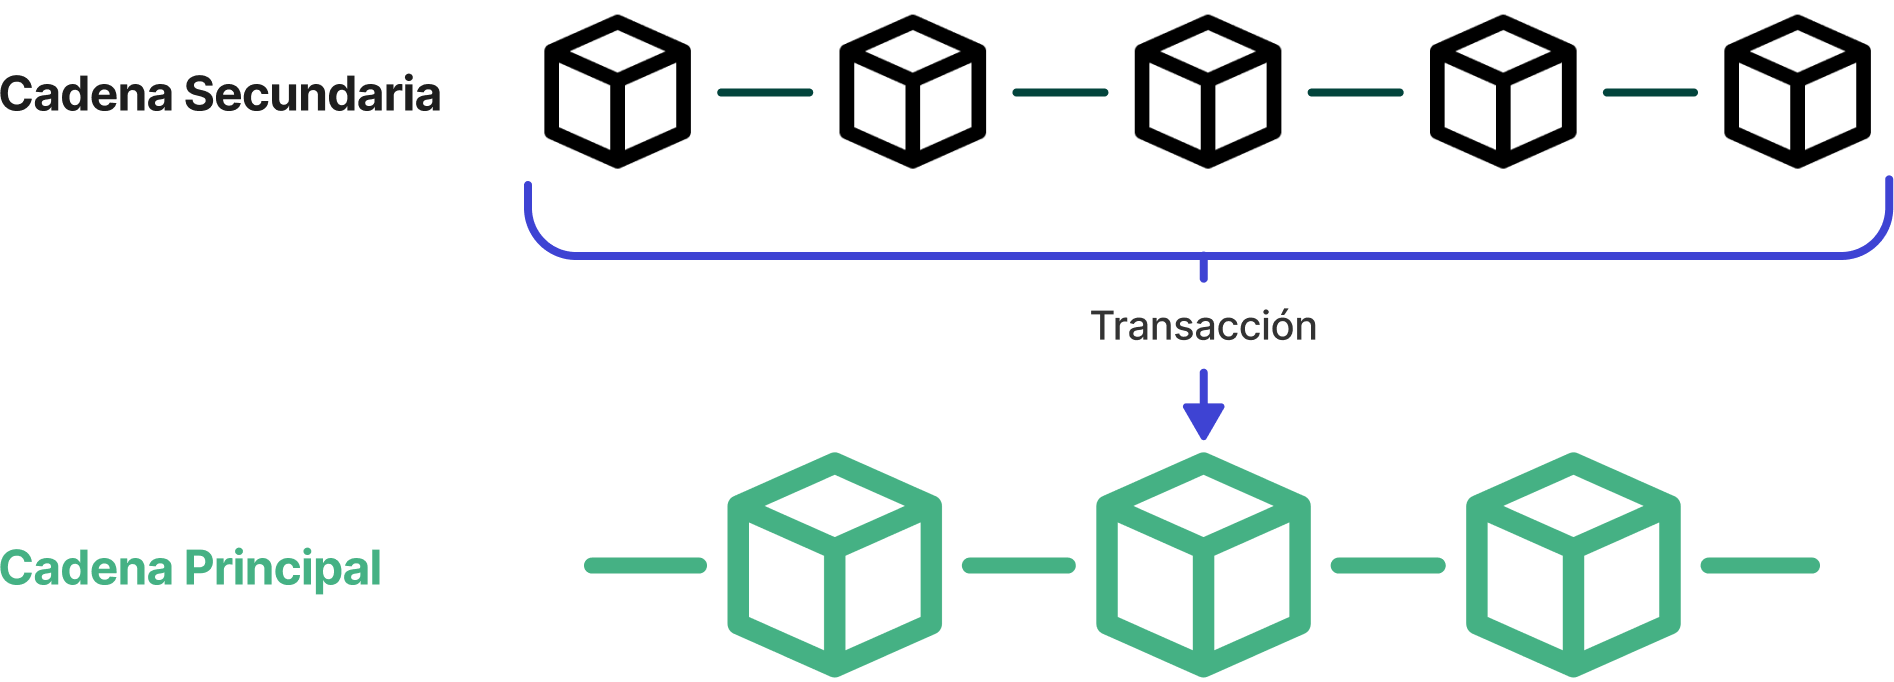
\includegraphics[width=0.9\linewidth]{Figures/blockchain-layer-2.png}
    \caption{Funcionamiento de una cadena secundaria sobre Ethereum}
    \label{fig:ethereum-layer-2}
\end{figure}

Sin embargo, Ethereum presenta algunas desventajas, como los altos costos de transacción y alta latencia de red, que pueden afectar la experiencia del usuario y la viabilidad económica del sistema. Afortunadamente, en la actualidad existen múltiples soluciones para mitigar estos problemas. En particular, para mitigar los altos costos y la latencia de la red de Ethereum para esta aplicación de trazabilidad que puede alcanzar un volumen de datos considerable, se decidió realizar el despliegue de los contratos en una cadena secundaria de Ethereum, que permite procesar las transacciones en una cadena complementaria de alto rendimiento y bajo costo para luego sincronizarla con la cadena principal mediante una única transacción (Figura \ref{fig:ethereum-layer-2}), lo que reduce costos y aumenta la escalabilidad, sin comprometer la seguridad ni la integridad de los datos de la \textit{blockchain} Ethereum. A su vez, se eligió hacer uso del \textit{framework} Hardhat\footnote{\url{https://hardhat.org}} para el desarrollo y despliegue de los \glspl{contratointeligente}, ya que es una herramienta ampliamente adoptada que facilita la implementación y ejecución de pruebas unitarias y de integración sobre contratos inteligentes en Solidity.

\subsection{Capa backend}

La capa de lógica de negocio, generalmente conocida como \textit{\gls{backend}} o \gls{api} (\textit{Application Programming Interface}), actúa como el cerebro del sistema. Su propósito principal es implementar y ejecutar las reglas de negocio del sistema, orquestar la interacción entre las distintas capas (capa \textit{frontend} y capa de datos), y exponer una interfaz estandarizada a través de la cual otros componentes puedan interactuar con la funcionalidad del sistema, sin depender de su implementación interna.

Para este prototipo, se ha optado por implementar una arquitectura desacoplada, donde la capa de presentación (\textit{frontend}) y la capa de lógica de negocio se desarrollan de forma independiente. Este tipo de arquitectura desacoplada resulta necesaria para un sistema de las características de este trabajo. A diferencia de una arquitectura monolítica, este enfoque promueve la modularidad y la escalabilidad, permitiendo que la interfaz de usuario pueda evolucionar o ser reemplazada sin afectar la lógica de negocio central de la aplicación. Este diseño responde directamente al requerimiento no funcional de interoperabilidad (RNF-05), ya que la \gls{api} de trazabilidad está pensada para ser el punto de integración principal no solo para el \textit{frontend} del prototipo, sino también para sistemas de gestión preexistentes, dispositivos \gls{iot} y otras aplicaciones de terceros que pudieran surgir en el futuro para la \gls{trazabilidad} de procesos de la \gls{cadenadesuministro} y reciclaje de los envases de vidrio.

Para la implementación de la capa \textit{backend} se tomó la decisión de utilizar la tecnología Node.js\footnote{\url{https://nodejs.org/es}}, un entorno de ejecución del lenguaje JavaScript\footnote{\url{https://developer.mozilla.org/es/docs/Web/JavaScript}} que permite crear servidores, aplicaciones web, herramientas de línea de comandos y \textit{scripts}. A su vez, JavaScript es un lenguaje de programación de alto nivel, interpretado y dinámico, que es ampliamente conocido y utilizado para el desarrollo web tanto en \textit{frontend} como en \textit{backend}. Su curva de aprendizaje es relativamente baja y es el lenguaje que se utiliza para dar dinamismo a las páginas web. Sin embargo, su uso también se ha extendido al lado del servidor gracias a entornos de ejecución como Node.js, lo que ha permitido a los desarrolladores crear aplicaciones web completas utilizando un único lenguaje de programación. Su popularidad y amplia adopción en la industria, se deben a su flexibilidad y a la gran cantidad de librerías y \textit{frameworks} que se han desarrollado para este lenguaje, que permiten construir tanto aplicaciones web simples, como sistemas complejos y escalables.

Existen múltiples motivos que justifican la elección del entorno Node.js para el desarrollo de la capa \textit{backend} de este trabajo. En primer lugar, considerando el alcance limitado del trabajo, JavaScript resulta ser un lenguaje propicio debido a su baja curva de aprendizaje y su flexibilidad para ser utilizado tanto en la capa \textit{backend} como en la capa \textit{frontend}, lo que facilita el proceso de desarrollo al permitir que el mismo desarrollador trabaje en ambas capas sin necesidad de cambiar de lenguaje. Existen múltiples lenguajes y \textit{frameworks} ampliamente utilizados en la industria para desarrollar la capa \textit{backend} de aplicaciones web, como Java con Spring Boot, Python con Django o Flask y Ruby on Rails, pero la posibilidad de utilizar el mismo lenguaje tanto en \textit{frontend} como en \textit{backend}, simplifica el proceso de desarrollo en equipos pequeños o unipersonales y ayuda a facilitar el mantenimiento del código en el futuro. A su vez, Node.js ofrece un excelente soporte para la interacción con la red de Ethereum, mediante una serie de librerías ampliamente adoptadas y probadas en la comunidad, como pueden ser Ethers.js y Web3.js. Por último, la amplia adopción de Node.js en la industria y la disponibilidad de herramientas para pruebas unitarias facilitan el desarrollo y el mantenimiento del sistema. 

\begin{figure}[!tb]
    \centering
    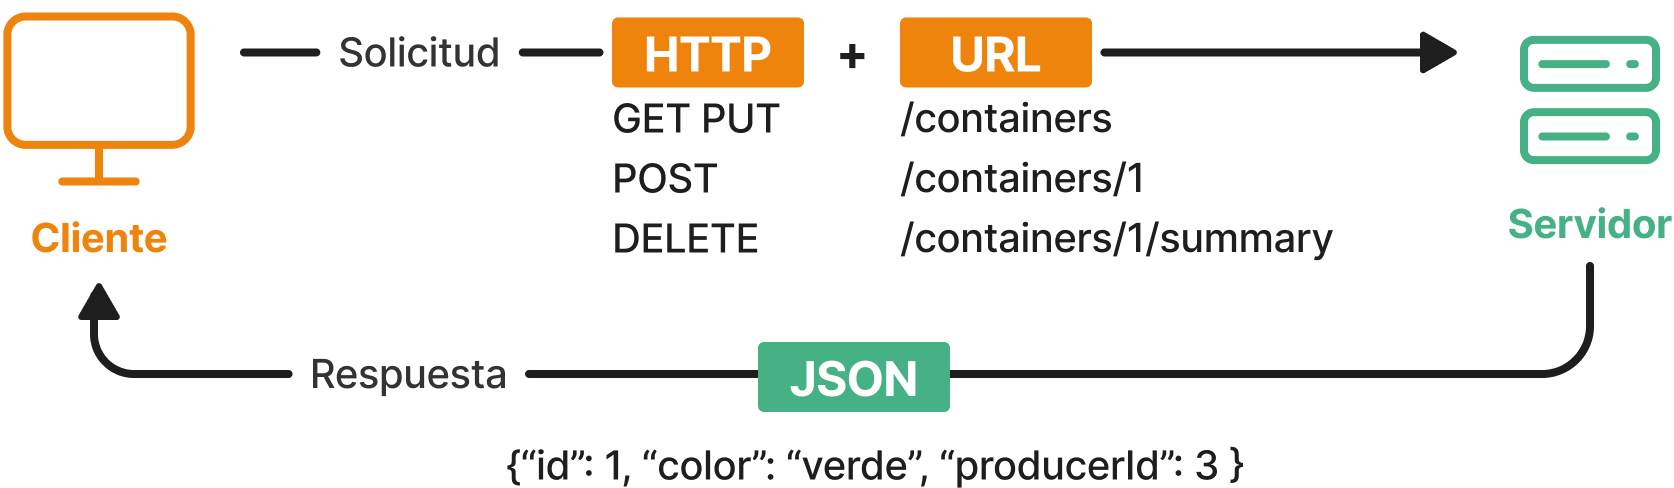
\includegraphics[width=\linewidth]{Figures/backend-api-rest.png}
    \caption{Funcionamiento de una API REST}
    \label{fig:api-rest}
\end{figure}

Por otro lado, la comunicación del \textit{backend} con las demás capas del sistema debe implementarse a través de interfaces bien definidas. La \gls{api} \textit{backend} implementa el estándar \textit{\gls{apirest}} para la comunicación con la capa de presentación. El estándar \acrshort{rest} (\textit{\acrlong{rest}}), ilustrado en la Figura \ref{fig:api-rest}, define una arquitectura para la comunicación entre sistemas que se basa en el uso del protocolo \gls{http} para intercambiar información sin mantener un estado entre intercambios. Una \gls{apirest} utiliza los métodos estándar de \gls{http} (como \textit{GET}, \textit{POST}, \textit{PUT} y \textit{DELETE}) para realizar operaciones sobre los recursos del sistema y adopta el formato \gls{json} para el intercambio de datos. La \gls{api} se estructura en un conjunto de \textit{\glspl{endpoint}}, cada uno representando una acción sobre un recurso específico del sistema, ya sea crear, leer, actualizar o eliminar el recurso. Por ejemplo, el \textit{frontend} del sistema podría enviar una solicitud \textit{GET} al \textit{endpoint} ``/api/containers'' para solicitar la lista de envases de vidrio producidos por cierto productor primario. En este caso, el \textit{backend} respondería con la información solicitada en formato \gls{json} y el \textit{frontend} podría utilizar esta información para actualizar la interfaz de usuario, mostrando el listado de los envases de vidrio correspondientes al usuario.

Dentro del entorno de Node.js, existen múltiples librerías y \textit{frameworks} que facilitan el desarrollo de \glspl{apirest}. La opción más popular y ampliamente adoptada es Express.js\footnote{\url{https://expressjs.com/}}, un \textit{framework} minimalista y flexible que proporciona las utilidades esenciales para la construcción de \glspl{apirest}. Entre sus principales ventajas se encuentran su simplicidad, flexibilidad y extensibilidad. Gracias a estas características, Express.js es utilizado para construir \gls{apirest} directamente, pero también ha sido utilizado como base de múltiples \textit{frameworks} de desarrollo de \glspl{apirest} más complejos, como Nest.js y Sails.js, entre otros. Estos \textit{frameworks} extienden las funcionalidades de Express.js y facilitan el desarrollo de \glspl{api} en Node.js, añadiendo funcionalidades adicionales que mejoran la mantenibilidad y escalabilidad de las \glspl{apirest}. Sin embargo, estos \textit{frameworks} suelen imponer una estructura más rígida y una curva de aprendizaje más pronunciada que Express.js. Por este motivo, se decidió utilizar Express.js como base para el desarrollo de la \gls{api} del sistema, ya que no impone restricciones adicionales sobre el modelo arquitectónico y permite una implementación eficiente y escalable, sin sacrificar la flexibilidad necesaria para adaptarse a los requerimientos específicos del sistema.

Finalmente, para la interacción con la capa de datos, el \textit{backend} se conecta a la base de datos relacional mediante librerías de conexión estandarizadas y a la \textit{blockchain} a través de librerías de interacción con \glspl{contratointeligente}, lo que permite un acceso unificado a los datos, abstrayendo la complejidad de cada fuente de datos y proporcionando una interfaz coherente para la capa \textit{frontend} del sistema.

\subsection{Capa frontend}

La capa de presentación, conocida habitualmente como \textit{\gls{frontend}}, es la interfaz de usuario web que permite a los distintos actores de la cadena de suministro interactuar con el sistema de trazabilidad del vidrio. Su objetivo es traducir la lógica de negocio y los datos que provienen de la API en una experiencia visual y funcional, permitiendo que los usuarios interactúen con el prototipo de manera intuitiva. El \textit{frontend} es la cara visible del sistema completo.

Para este prototipo, se tomó la decisión de implementar de forma desacoplada la interfaz de la lógica de negocio, con el objetivo de reforzar la mantenibilidad y flexibilidad del sistema. Esta separación es propicia para que la interfaz de usuario pueda evolucionar de manera independiente de la lógica, adaptándose a nuevas necesidades, experiencias de usuario o tecnologías sin afectar el funcionamiento del sistema. Con este esquema, es factible que en un futuro, cada actor de la cadena tenga acceso a una interfaz a medida de sus necesidades. Por ejemplo, para un productor de envases de vidrio, se podría desarrollar una aplicación de escritorio con métricas de negocio sobre su producción y venta, mientras que para los consumidores, se podría crear una aplicación móvil que muestre puntos de reciclaje y ofrezca incentivos por reciclar. Aunque el prototipo desarrollado para este trabajo final presenta una interfaz web unificada para todos los actores, el diseño modular facilita la creación de estas aplicaciones independientes en el futuro.

La elección tecnológica para esta capa estuvo focalizada en encontrar \textit{frameworks} y librerías que promuevan la modularidad y la eficiencia durante el desarrollo. En primer lugar, se determinó utilizar React\footnote{\url{https://es.react.dev/}} como librería base para la construcción de la interfaz, debido a su modelo de desarrollo basado en componentes, que promueve la reutilización de código. A su vez, para potenciar React, se optó por hacer uso del \textit{framework} Next.js\footnote{\url{https://nextjs.org/docs}}, que agrega funcionalidades extra a React para facilitar aún más el desarrollo de aplicaciones web modulares y de alto rendimiento, combinando técnicas como generación de sitios estáticos y renderizado en el servidor. Por otro lado, para el diseño de las interfaces web se utiliza el lenguaje de estilado \gls{css}\footnote{\url{https://developer.mozilla.org/en-US/docs/Web/CSS}}, que en este prototipo se complementó con el uso de la librería Tailwind \gls{css}\footnote{\url{https://tailwindcss.com/}} que promueve una estética moderna y una sintaxis simplificada dentro del código.

La comunicación del \textit{frontend} con el \textit{\gls{backend}} se realiza exclusivamente a través de llamadas a la \gls{apirest}. La interfaz no contiene la lógica de negocio, sino que actúa como un cliente ligero que envía datos al \textit{backend} (por ejemplo, al registrar un nuevo lote) y recibe la respuesta, la cual es luego presentada al usuario. Este modelo garantiza que el \textit{frontend} se enfoque en la interacción y la visualización, mientras la lógica crítica reside en el \textit{backend}. Debido a que el \textit{frontend} se enfoca únicamente en la visualización de información, es necesario implementar un sistema de autenticación y autorización unificado entre \textit{frontend} y \textit{backend} que permita a cada usuario visualizar e interactuar únicamente con las funcionalidades propias de su rol. Por este motivo, para gestionar la autenticación de usuarios en este proyecto, se determinó hacer uso del servicio Firebase Authentication\footnote{\url{https://firebase.google.com/docs/auth}}, que gestiona la autenticación de usuarios e implementa de forma abstracta el estándar de autorización OAuth 2.0\footnote{\url{https://oauth.net/2/}}, asegurando que solo los actores con los permisos adecuados puedan acceder a cada recurso del sistema.

\begin{figure}[!t]
    \centering
    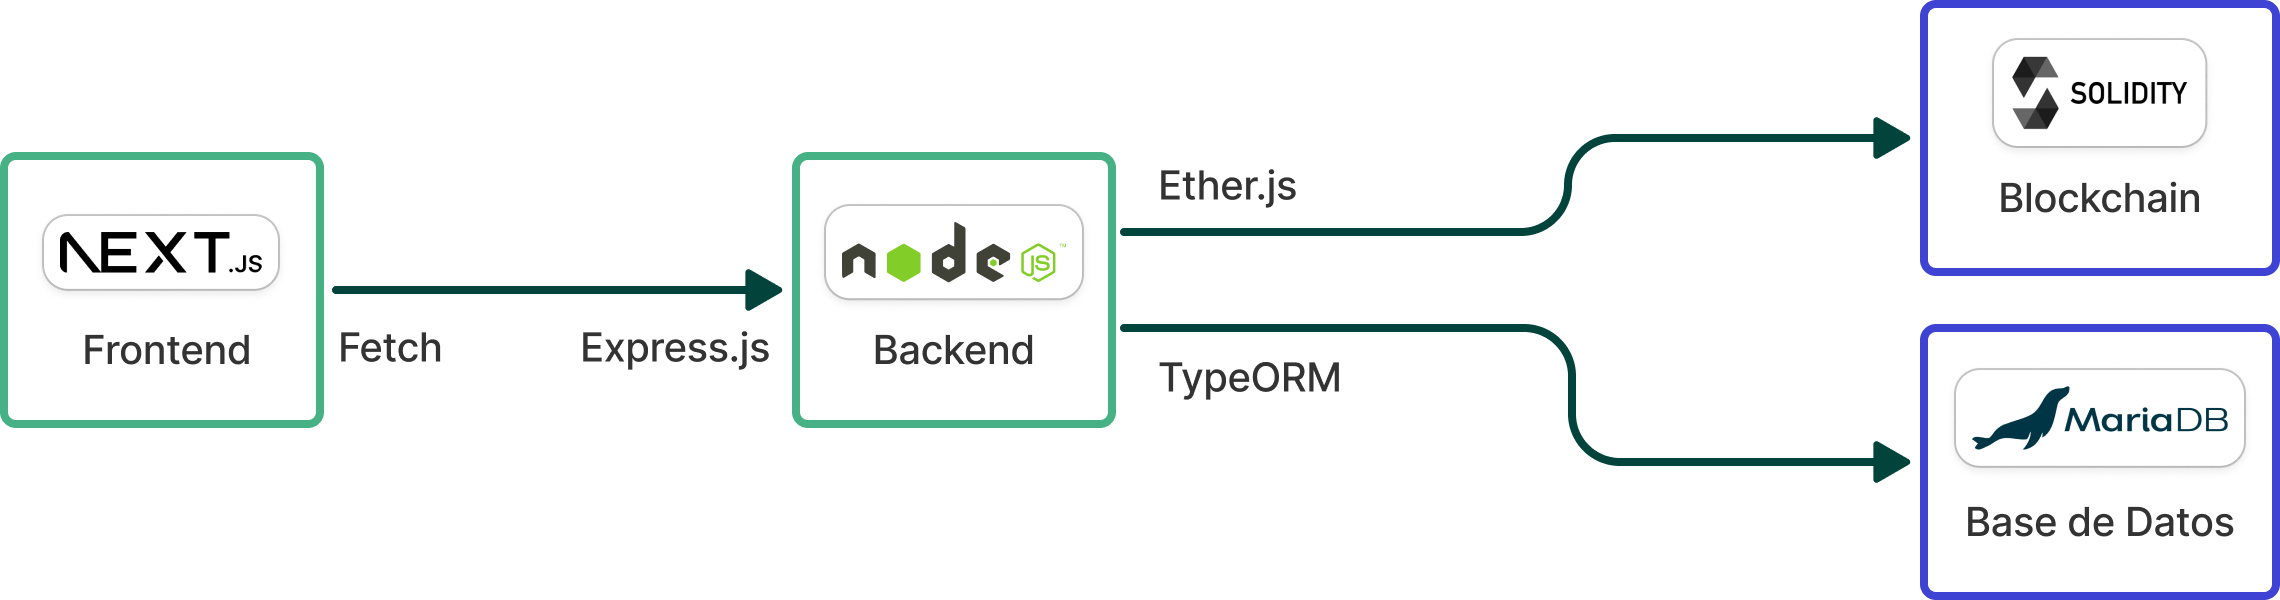
\includegraphics[width=\linewidth]{Figures/system-architecture.png}
    \caption{Arquitectura del sistema con librerías elegidas para comunicación entre módulos}
    \label{fig:system-architecture}
\end{figure}

Por último, en la Figura \ref{fig:system-architecture} se puede observar la arquitectura general del sistema, donde Next.js se utiliza para el desarrollo del \textit{frontend}, que se comunica con el \textit{backend}, que se implementa en Node.js y utiliza el \textit{framework} Express.js para recibir las solicitudes, mientras que emplea librerías específicas para comunicarse con los contratos inteligentes en Solidity y con la base de datos relacional de MariaDB. 
Luego de definir la arquitectura de la aplicación web, incluyendo la definición de capas, la comunicación entre ellas y los lenguajes de programación a utilizarse, es posible comenzar con la etapa de diseño de componentes. En esta segunda etapa de diseño, se define la arquitectura interna de cada capa o módulo definido en la etapa anterior. En la próxima sección, se detallará el diseño de componentes de este sistema, que abarca la estructura interna del \textit{frontend}, la API y la capa de datos.

\section{Diseño de componentes}
\label{sec:components-design}

La segunda etapa de diseño, el diseño de componentes, tiene como objetivo detallar la arquitectura interna de los módulos definidos en la fase anterior. Su propósito es traducir la arquitectura de alto nivel en un plan de construcción específico, que incluye la estructura de la interfaz de usuario, la arquitectura de la API y el modelo de datos. Esta fase toma como punto de partida los requerimientos del sistema y la arquitectura de módulos previamente definida, y su resultado es un conjunto de especificaciones detalladas que guiarán la implementación de cada módulo del software. De esta forma, se busca asegurar la cohesión interna de cada módulo y su correcta interacción con los demás. A su vez, cada decisión de diseño tomada en esta etapa se verificará posteriormente en la fase de pruebas de integración, que valida la correcta comunicación entre los componentes del sistema.

A continuación, se presentarán las decisiones de diseño tomadas para cada uno de los módulos definidos en la arquitectura del sistema: la capa de datos, la capa de lógica de negocio (\textit{backend}) y la capa de presentación (\textit{frontend}).

\subsection{Arquitectura de datos}

El diseño de la arquitectura de datos representa un componente central de este trabajo, ya que debe integrar de manera transparente y eficiente la naturaleza descentralizada de la \textit{blockchain} con la eficiencia y escalabilidad de una \gls{basededatos} relacional para cumplir con los requerimientos no funcionales del sistema (RNF-01: Transparencia, RNF-03: Escalabilidad y RNF-06: Integridad). La solución definida durante la etapa de diseño de arquitectura propone un modelo de datos híbrido para optimizar el almacenamiento y la recuperación de información. En este esquema, la \textit{blockchain} se utiliza como una capa de confianza inmutable, mientras que la base de datos relacional se encarga de la gestión de datos auxiliares que no requieren la inmutabilidad de la cadena de bloques. El diseño de componentes para esta arquitectura, por lo tanto, implica definir la estructura de los contratos inteligentes en la \textit{blockchain} y el esquema de la base de datos relacional, asegurando que ambos sistemas interactúen de manera eficiente y coherente.

\begin{figure}[!tb]
    \centering
    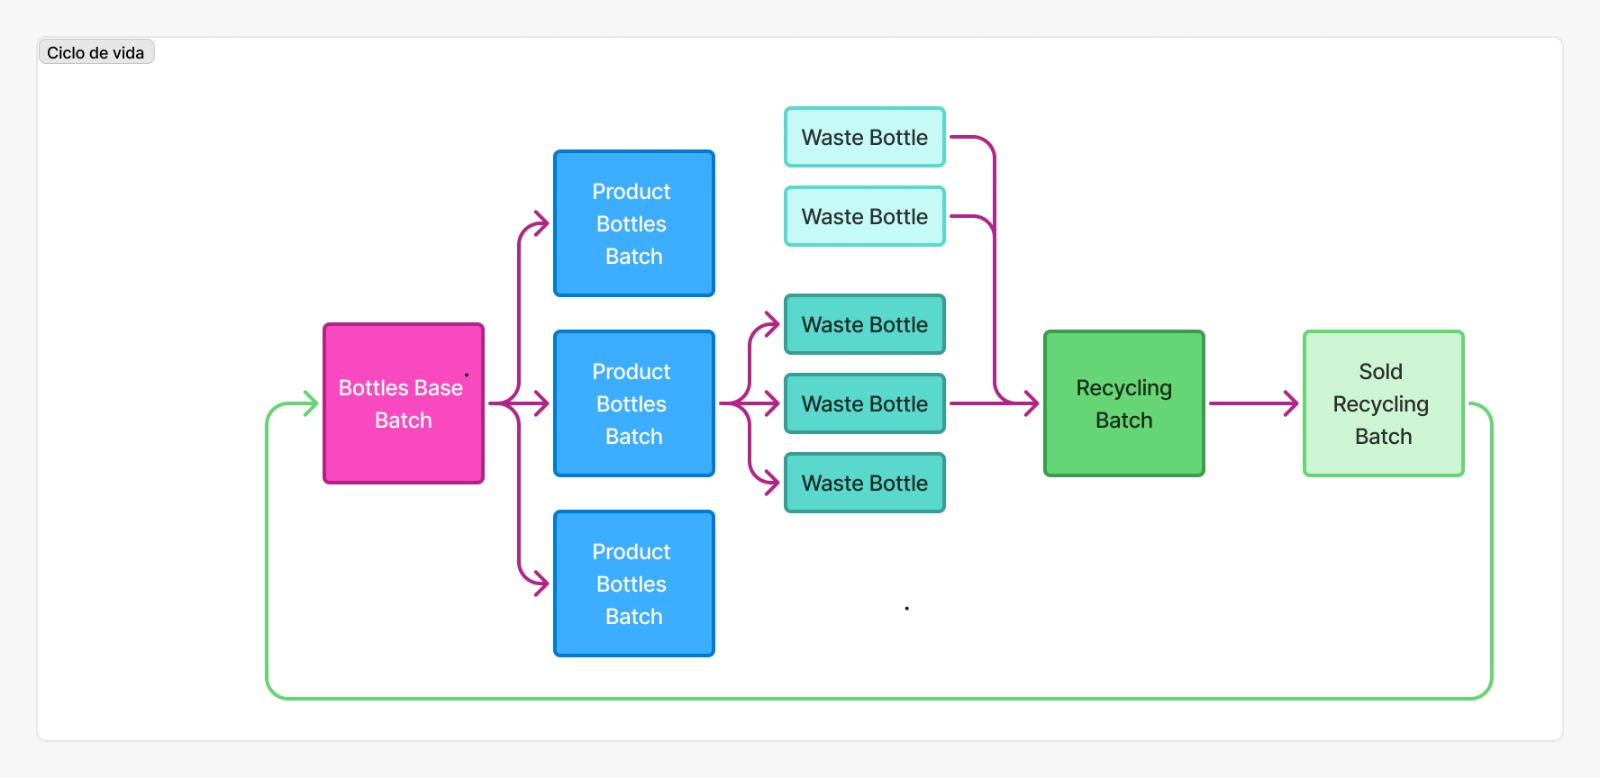
\includegraphics[width=\linewidth]{Figures/data-lifecycle.png}
    \caption{Diagrama de ciclo de vida de los envases de vidrio en el sistema}
    \label{fig:data-lifecycle}
\end{figure}

En primera instancia, se definió la representación de los datos, tanto en la \textit{blockchain} como en la base de datos relacional. Con base en los requerimientos del sistema y la investigación sobre el ciclo de vida del vidrio, se optó por representar cada envase o conjunto de envases con una estructura distinta en cada etapa de su vida útil. Esta decisión se tomó debido a que los envases tienen metadatos, propietarios y agrupaciones diferentes en cada fase del proceso. El flujo de estados de los envases de vidrio, como se observa en la Figura \ref{fig:data-lifecycle}, comienza con un lote de envases producido por el productor primario, que luego se vende a múltiples productores secundarios para crear lotes de productos envasados. Finalmente, los consumidores pueden llevar cada envase vacío a centros de reciclaje, donde se agrupan en lotes de reciclaje para su posterior reprocesamiento. Para mantener la \gls{trazabilidad} completa del ciclo de vida, cada elemento posee una referencia a su ID (identificador) de origen, lo que permite rastrear, a partir de un envase reciclado, el lote original en el que fue producido, su productor y sus metadatos.

\begin{figure}[!b]
    \centering
    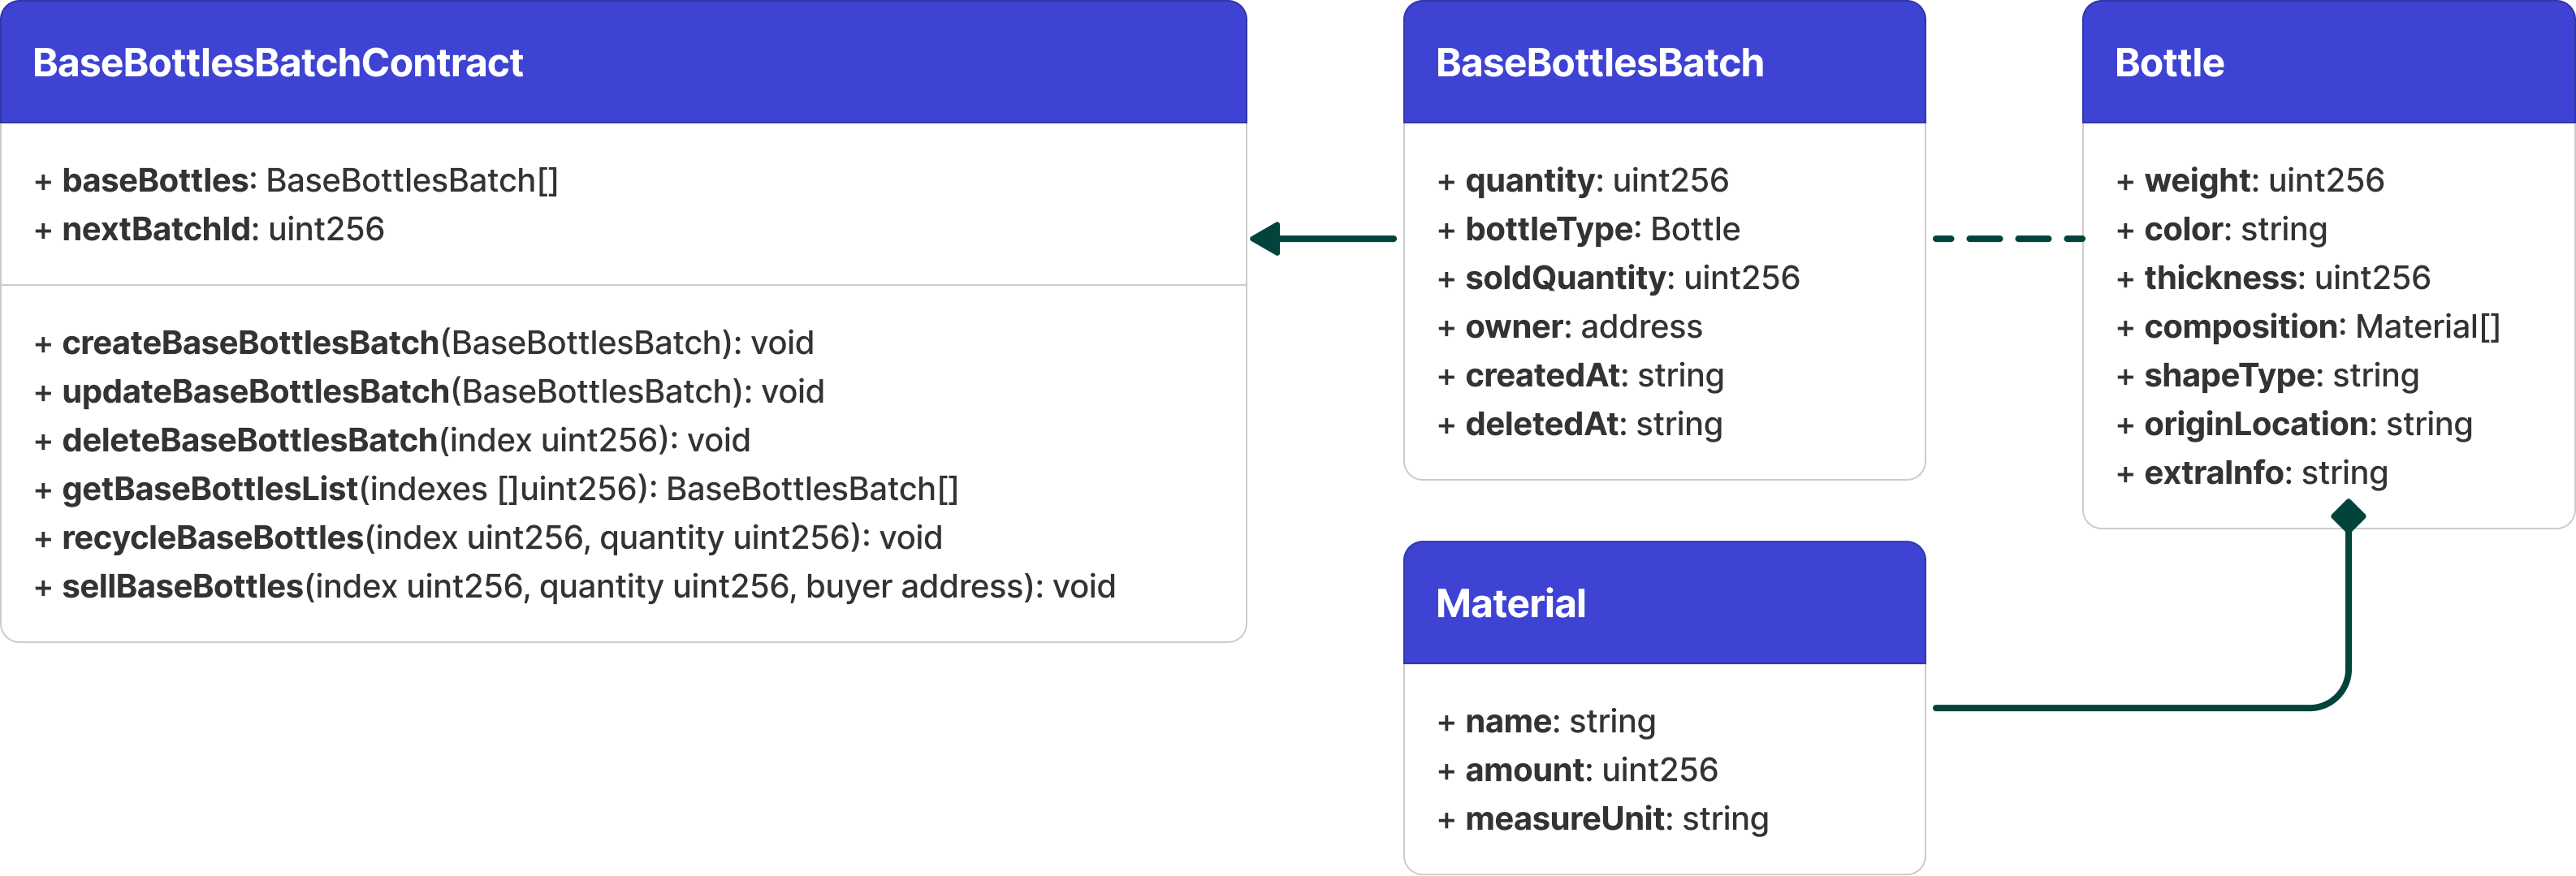
\includegraphics[width=\linewidth]{Figures/uml-producer-contract.png}
    \caption{Diagrama \acrshort{uml} del Contrato de Envases (BaseBottlesBatchContract)}
    \label{fig:bottles-contract-uml}
\end{figure}

A partir de la representación de los datos, se diseñaron los \glspl{contratointeligente} en la \textit{blockchain} para almacenar únicamente la información necesaria para garantizar la trazabilidad de los envases y la integridad de los datos, como un identificador único de cada lote de vidrio, sus metadatos esenciales de producción, el propietario actual y un historial de las transferencias de propiedad y de estado. Al igual que en un sistema de programación orientada a objetos (\gls{oop}), los contratos en Solidity implementan atributos que guardan el estado y métodos que permiten interactuar con él. En lugar de un único contrato monolítico, se decidió implementar tres contratos que interactúan entre sí para lograr mayor modularidad, mantenibilidad y desacoplamiento. A continuación, se detalla la arquitectura de cada uno de ellos, incluyendo sus responsabilidades y la interacción entre ellos. Para cada contrato, se presenta un diagrama de clases \acrshort{uml} (\textit{\acrlong{uml}}) que ilustra su estructura interna, junto con las estructuras de datos relacionadas. Un diagrama de clases \acrshort{uml} es una herramienta visual que se usa en la \gls{ingenieriadesoftware} para modelar la estructura de un sistema orientado a objetos. Describe las clases con sus atributos (datos) y métodos (funciones), y las relaciones entre ellas. Permite visualizar la composición y las interacciones del sistema, facilitando la comunicación y el entendimiento entre los desarrolladores. De forma práctica, actúa como un mapa conceptual que detalla los componentes principales del software antes de su implementación. Dentro del diagrama, los nombres de clases y propiedades se describen en inglés, siguiendo las convenciones de nomenclatura estándar vigentes en programación en entornos profesionales. Posteriormente, en la etapa de codificación, todo el código será implementado en inglés siguiendo este estándar, por lo que se utilizarán los nombres definidos en los diagramas \acrshort{uml} para mantener la coherencia y facilitar la comprensión del código.

\textbf{Contrato de envases: BaseBottlesBatchContract} (Figura \ref{fig:bottles-contract-uml})
 es el punto de partida del ciclo de vida del vidrio, encargado de gestionar la producción inicial de los envases. Sus responsabilidades incluyen registrar lotes de botellas recién fabricadas por el productor primario y sus metadatos (como la cantidad y composición), así como gestionar la transferencia de propiedad a productores secundarios. Sus métodos permiten crear, actualizar y eliminar lotes, además de consultar la información histórica de los mismos. La información de este contrato es consumida por el  contrato \textit{ProductBottlesBatchContract}, proporcionando una referencia al lote original para el siguiente eslabón de la cadena de trazabilidad.

\begin{figure}[!tb]
    \centering
    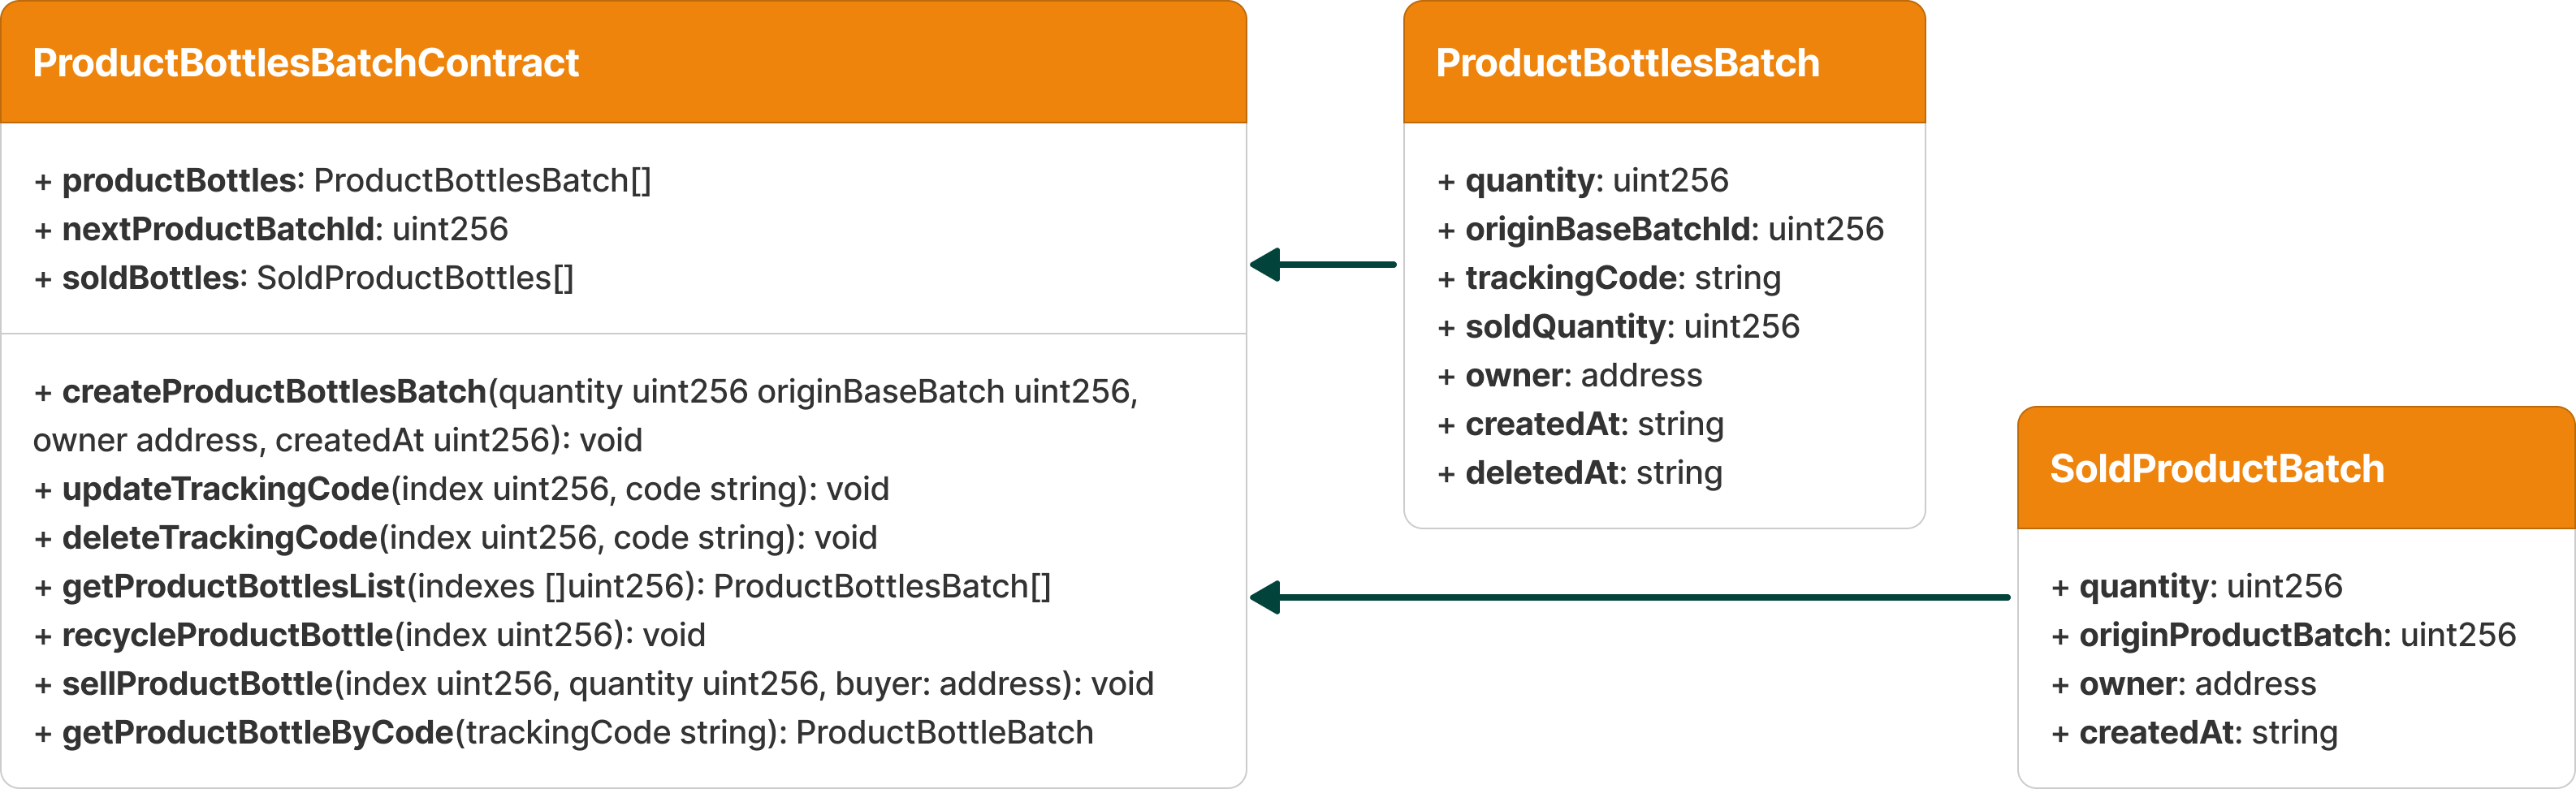
\includegraphics[width=\linewidth]{Figures/uml-product-contract.png}
    \caption{Diagrama \acrshort{uml} del Contrato de Productos (ProductBottlesBatchContract)}
    \label{fig:product-contract-uml}
\end{figure}

\begin{figure}[!b]
    \centering
    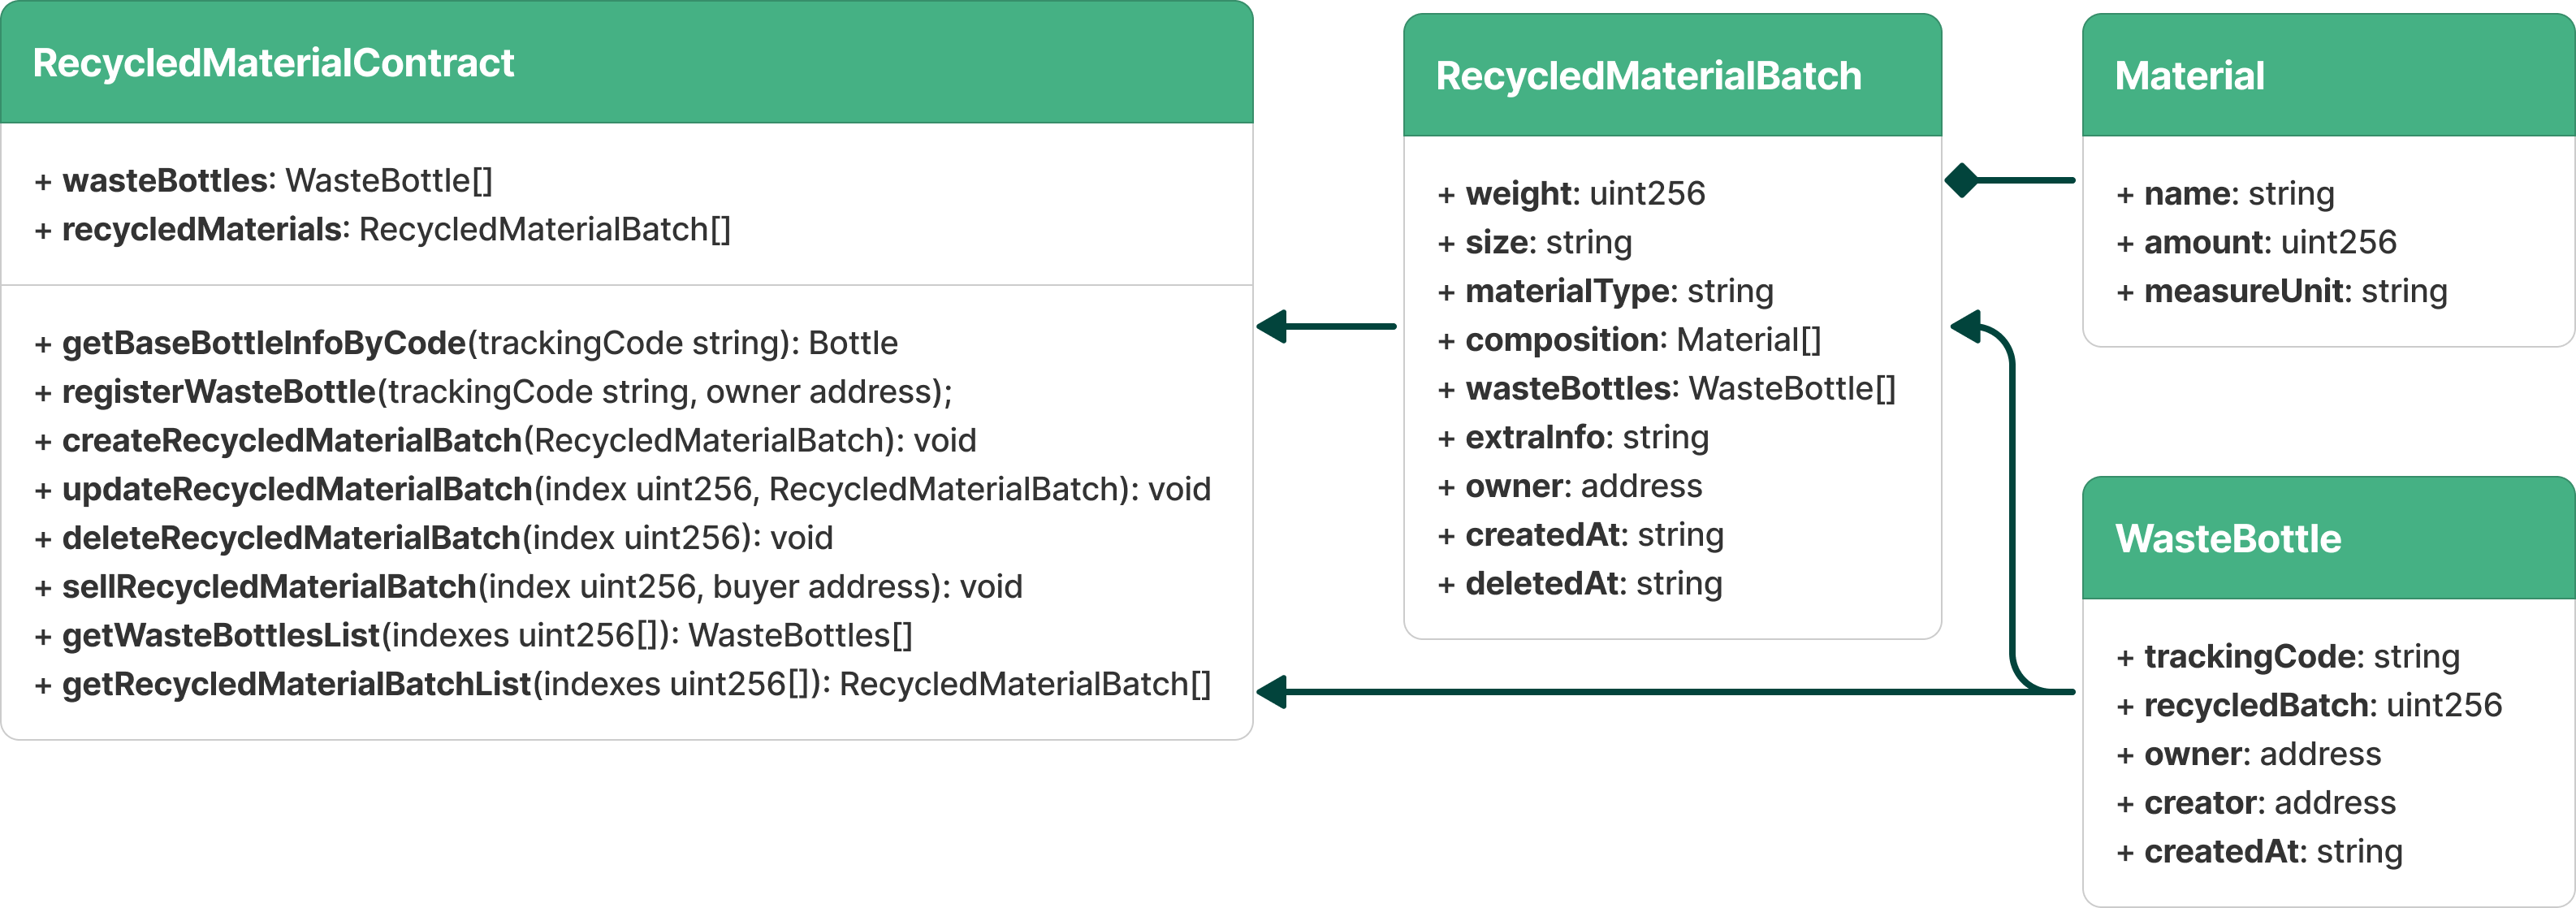
\includegraphics[width=\linewidth]{Figures/uml-recycling-contract.png}
    \caption{Diagrama \acrshort{uml} del Contrato de Reciclaje (RecycleMaterialContract)}
    \label{fig:recycling-contract-uml}
\end{figure}

\textbf{Contrato de productos: ProductBottlesBatchContract} (Figura \ref{fig:product-contract-uml})
 gestiona la segunda fase del ciclo de vida del vidrio, comprende el envasado y la comercialización de estos productos. Este contrato registra los lotes de productos terminados, asociando un código de seguimiento a cada uno y referenciando el lote de envases original del contrato \textit{BaseBottlesBatchContract}. Sus funciones permiten crear lotes de productos, registrar su venta y marcar aquellos envases que se convierten en residuos. La información de seguimiento generada en este contrato juega un rol central en el sistema de trazabilidad, ya que el código de seguimiento introducido en este contrato actúa como el eslabón intermedio que permite vincular el lote de origen de un envase de \textit{BaseBottlesBatchContract} con el envase en \textit{RecycleMaterialContract} cuando el consumidor lo desecha para su posterior reciclaje.

\textbf{Contrato de reciclaje: RecycleMaterialContract} (Figura \ref{fig:recycling-contract-uml})
 cubre la gestión del final de la vida útil de los envases, desde su recolección como residuo hasta su procesamiento como material reciclado. Este contrato almacena los registros de los envases que han sido entregados para reciclaje, permitiendo crear nuevos lotes de material reciclado a partir de ellos. Sus métodos permiten registrar envases de desecho, crear lotes de material reciclado (agrupando envases previamente registrados) y transferir la propiedad de estos lotes a los productores primarios, cerrando de esta forma el ciclo de vida circular del vidrio. La información de seguimiento de los envases provista por el contrato \textit{ProductBottlesBatchContract} es consumida por este contrato, que a su vez genera nuevos lotes de material que pueden ser reutilizados por el contrato \textit{BaseBottlesBatchContract}.

\begin{figure}[!b]
    \centering
    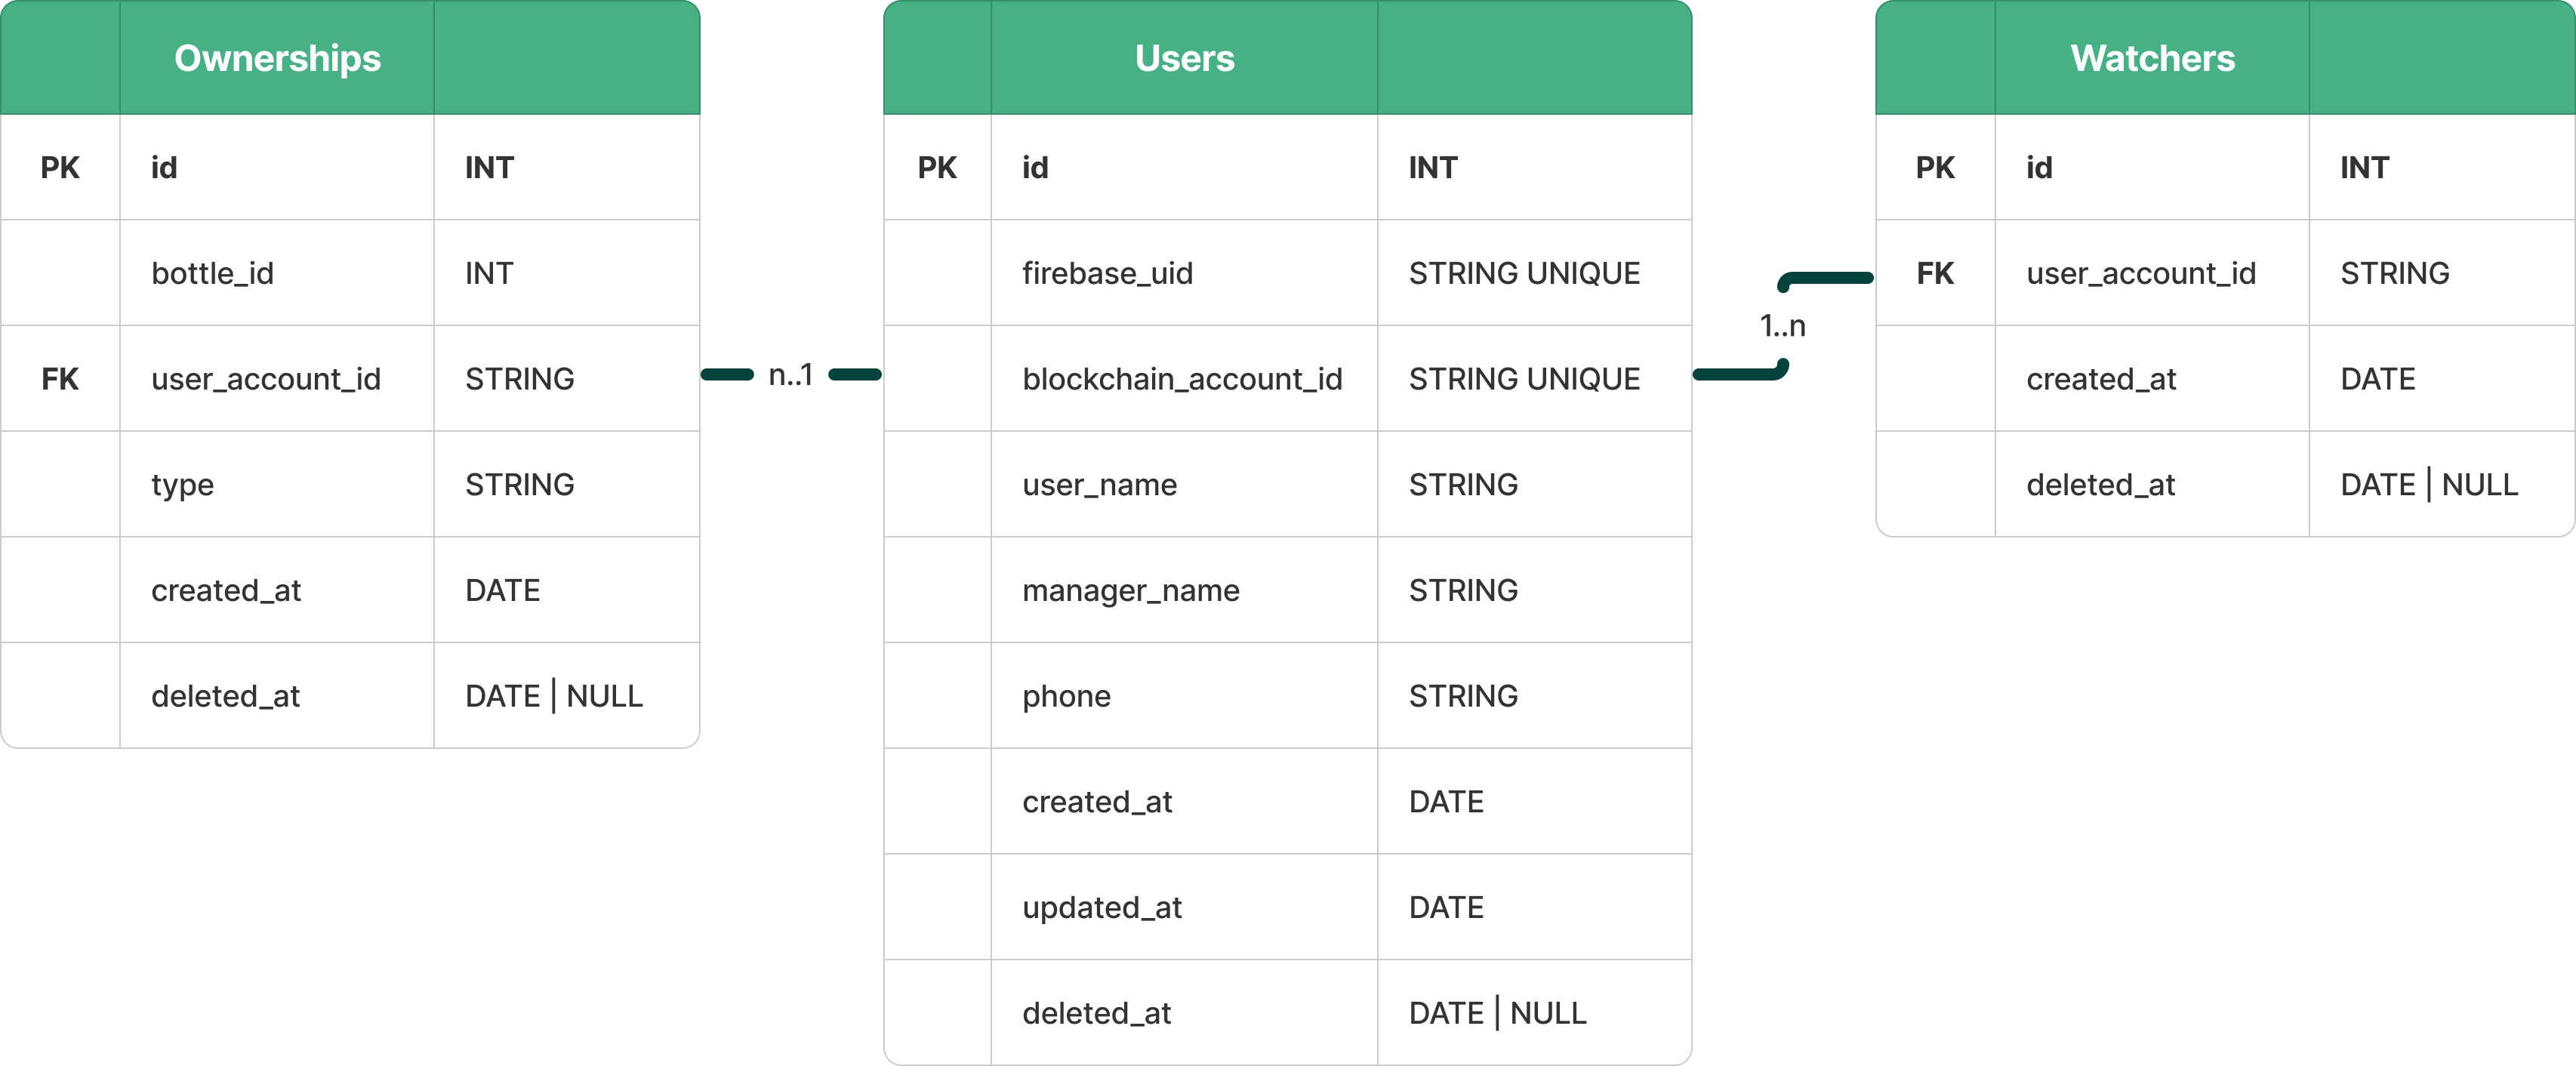
\includegraphics[width=\textwidth]{Figures/db-der.png}
    \caption{Diagrama Entidad-Relación (\gls{der}) del modelo de datos}
    \label{fig:der}
\end{figure}

De forma complementaria a la arquitectura de contratos inteligentes, el diseño de la \gls{basededatos} relacional almacena la información de los usuarios (relacionada con los requerimientos funcionales de autenticación y autorización) y una referencia al ID y propietario de cada lote y envase registrado en la \textit{blockchain}. La relación entre los datos de la \textit{blockchain} y la base de datos relacional se establece mediante el identificador único del lote, que sirve como clave de enlace y permite realizar consultas de metadatos detallados de cada lote. Adicionalmente, en la base de datos relacional se guarda una referencia a cada envase reciclado por los consumidores. Esto permite que cada consumidor pueda acceder al listado de envases que ha reciclado previamente y consultar si efectivamente ha sido procesado, cumpliendo así con el requerimiento funcional asociado (RF-023). En la Figura \ref{fig:der} se presenta un diagrama (DER) que ilustra la relación entre las entidades de la \gls{basededatos}.

\subsection{Arquitectura backend}

En el diseño de arquitectura de la capa \textit{\gls{backend}} se adoptó el patrón \textit{\Gls{cleanarchitecture}} (Arquitectura Limpia) \cite{martin2017clean}, un modelo de diseño que prioriza la separación de las reglas de negocio de las dependencias externas. En este esquema, la implementación de la API se estructura en tres capas principales: \textit{Routers}, \textit{Handlers} y \textit{Repositories}. Los \textit{routers} reciben las solicitudes HTTP y las dirigen a los \textit{handlers} correspondientes, luego los \textit{handlers} contienen la lógica de negocio y orquestan las operaciones, por último, los \textit{repositories} se encargan de la interacción con las fuentes de datos (ya sea la base de datos relacional o la \textit{blockchain}). La comunicación entre estas capas es unidireccional, lo que significa que las capas externas solo pueden acceder a las capas más internas, reforzando así la independencia de la lógica de negocio. La Figura \ref{fig:clean-architecture} ilustra cómo las interfaces externas (como el \textit{frontend} y otros sistemas) interactúan únicamente con los controladores (\textit{routers}), los cuales a su vez interactúan con los casos de uso (\textit{handlers}), que finalmente se comunican con las entidades (\textit{repositories}) para acceder al dominio (datos).

\begin{figure}[!b]
\centering
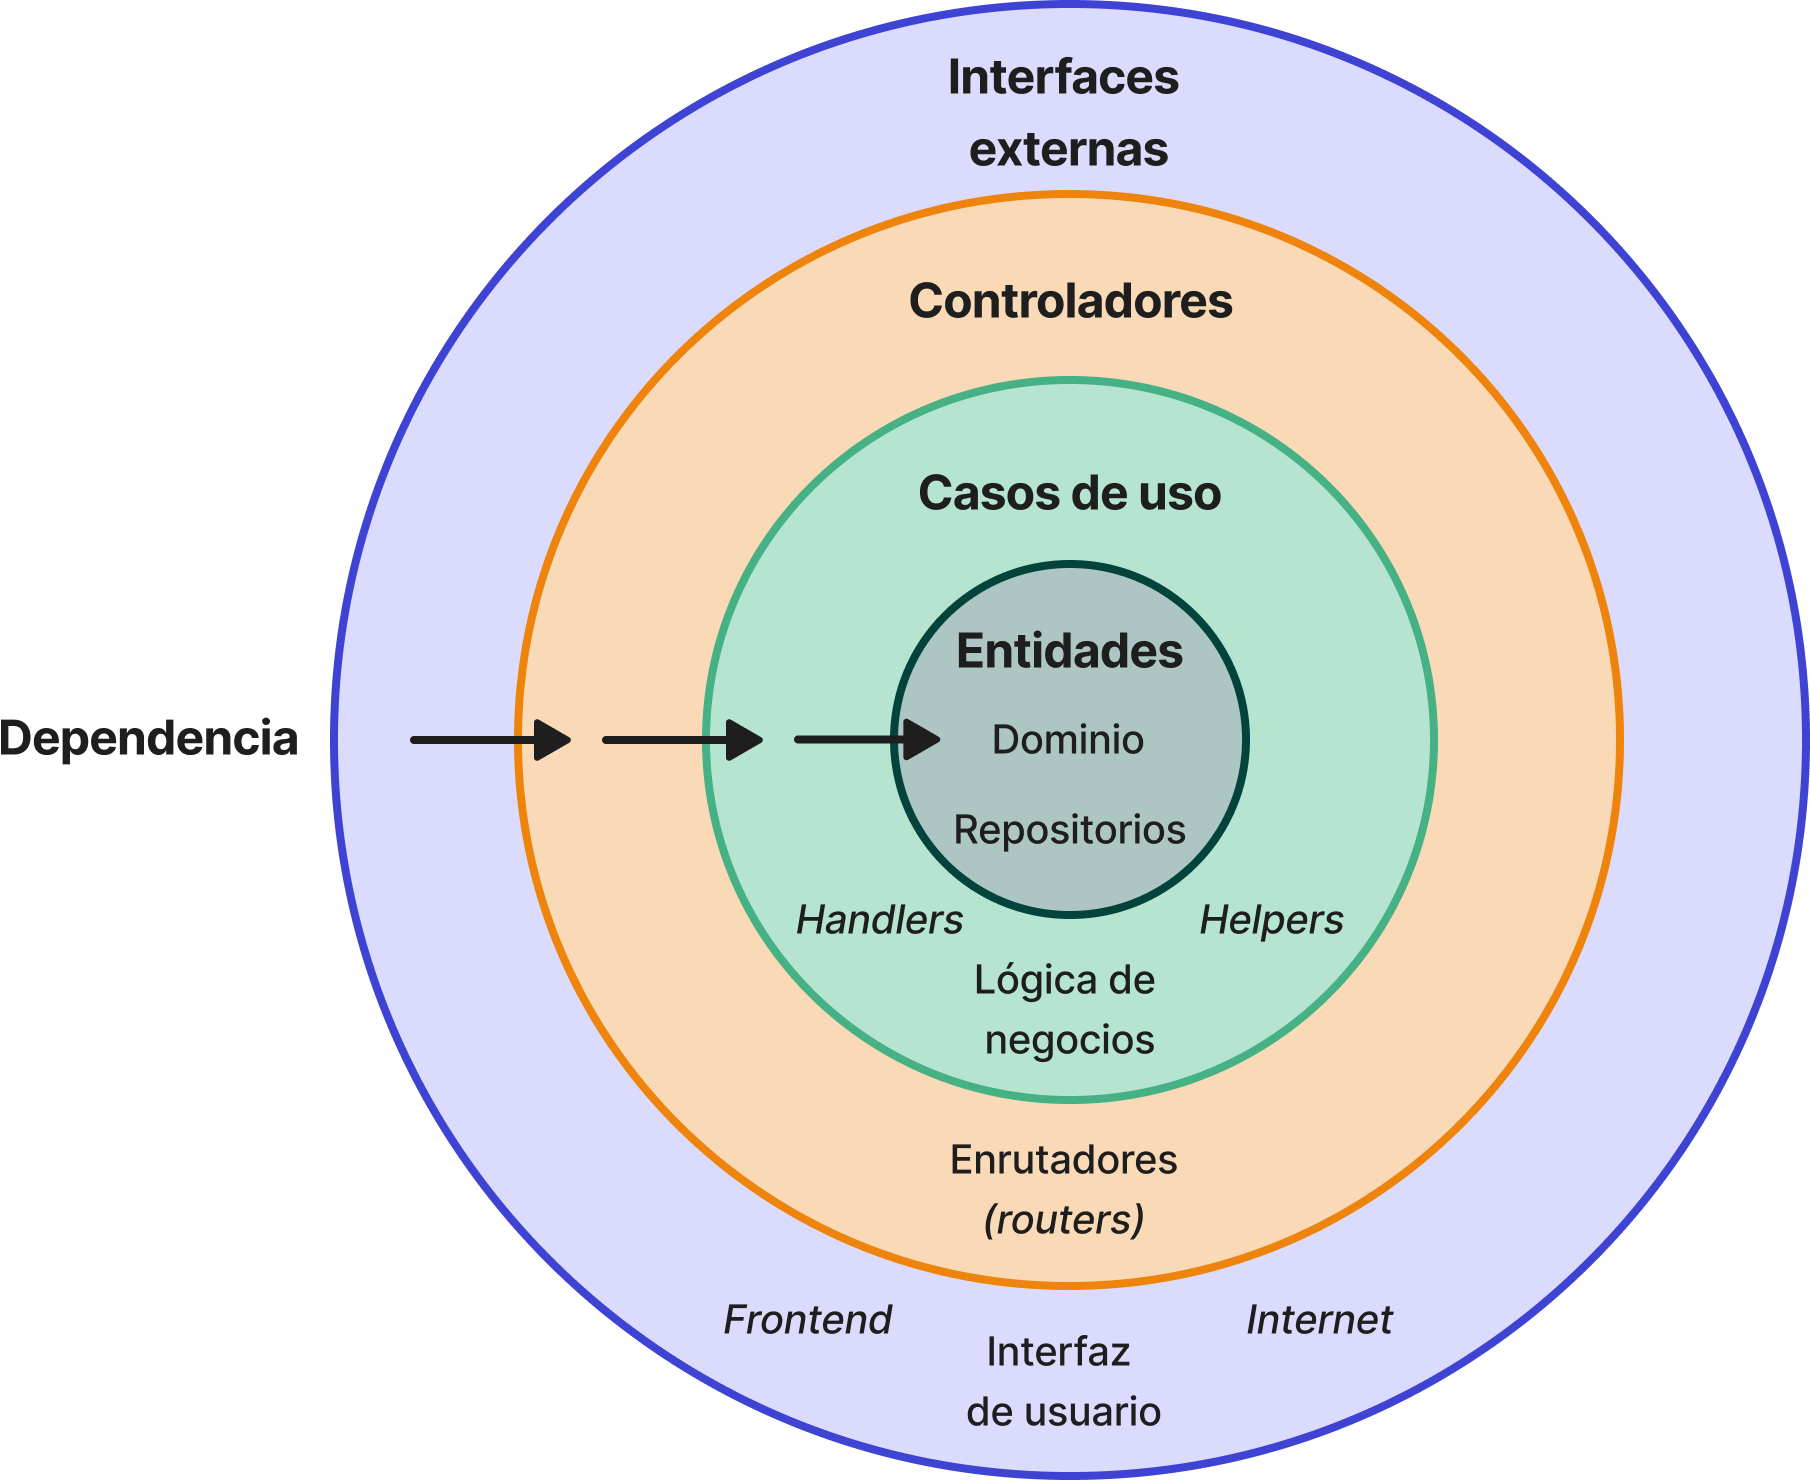
\includegraphics[width=0.6\textwidth]{Figures/clean-architecture.png}
\caption{Modelo \textit{Clean Architecture}}
\label{fig:clean-architecture}
\end{figure}

La elección del patrón \textit{\gls{cleanarchitecture}} se justifica por su capacidad para generar un sistema altamente desacoplado, lo que se traduce en una mayor mantenibilidad del sistema y flexibilidad ante futuros cambios. La lógica de negocio, situada en el núcleo de la arquitectura (\textit{Handlers}), se mantiene independiente de las tecnologías de implementación (infraestructura), la presentación de los datos (\textit{Routers}) y las bases de datos (\textit{Repositories}). Esto es particularmente ventajoso en un sistema de trazabilidad como el planteado en este trabajo, donde la lógica de negocio debe ser estable, pero la interfaz de usuario y las integraciones con otros sistemas (como plataformas de gestión o dispositivos \gls{iot}) pueden evolucionar. A su vez, en este proyecto la arquitectura de la API se ha dividido en módulos de dominio (por ejemplo, gestión de usuarios o trazabilidad de lotes), cada uno de los cuales expone un conjunto de \textit{\glspl{endpoint}} a través de una \gls{apirest}.

En particular, para orquestar la comunicación entre la API, la base de datos relacional y la \textit{blockchain}, se implementó un patrón de repositorios que unifica las operaciones de lectura y escritura. De esta forma, el \textit{handler} puede manejar todos los datos de manera uniforme, sin importar si el repositorio los obtuvo de la \textit{blockchain} o de la base de datos relacional, ya que esta lógica de acceso a datos se abstrae en el repositorio. Por ejemplo, al registrar un nuevo lote, el \textit{handler} valida la información y luego instruye al repositorio de la \textit{blockchain} para registrar la transacción y al repositorio de la base de datos relacional para almacenar la referencia del lote. En este caso, el patrón de diseño \textit{Clean Architecture} permite abstraer la complejidad de la arquitectura híbrida, proporcionando una interfaz de programación unificada a la capa de lógica de negocio.

\subsection{Arquitectura frontend}

La interfaz de usuario del sistema se diseñó como una aplicación web, con el objetivo de proporcionar una experiencia de usuario fluida, accesible desde cualquier dispositivo con conexión a Internet y sin necesidad de instalar software adicional. Debido al alcance limitado del trabajo, se decidió implementar una interfaz diseñada para computadoras de escritorio, dado que es el caso de uso más frecuente en sistemas de gestión y trazabilidad. La aplicación podrá accederse en dispositivos móviles, pero no se ha priorizado la implementación adaptada para estos dispositivos, por lo que la interfaz puede resultar menos amigable en pantallas pequeñas. La interfaz se estructuró mediante una arquitectura basada en componentes, un patrón de diseño que promueve la creación de elementos reutilizables, modulares e independientes, que es el patrón recomendado por librerías como React y \textit{frameworks} como Next.js.

\begin{figure}[!t]
\centering
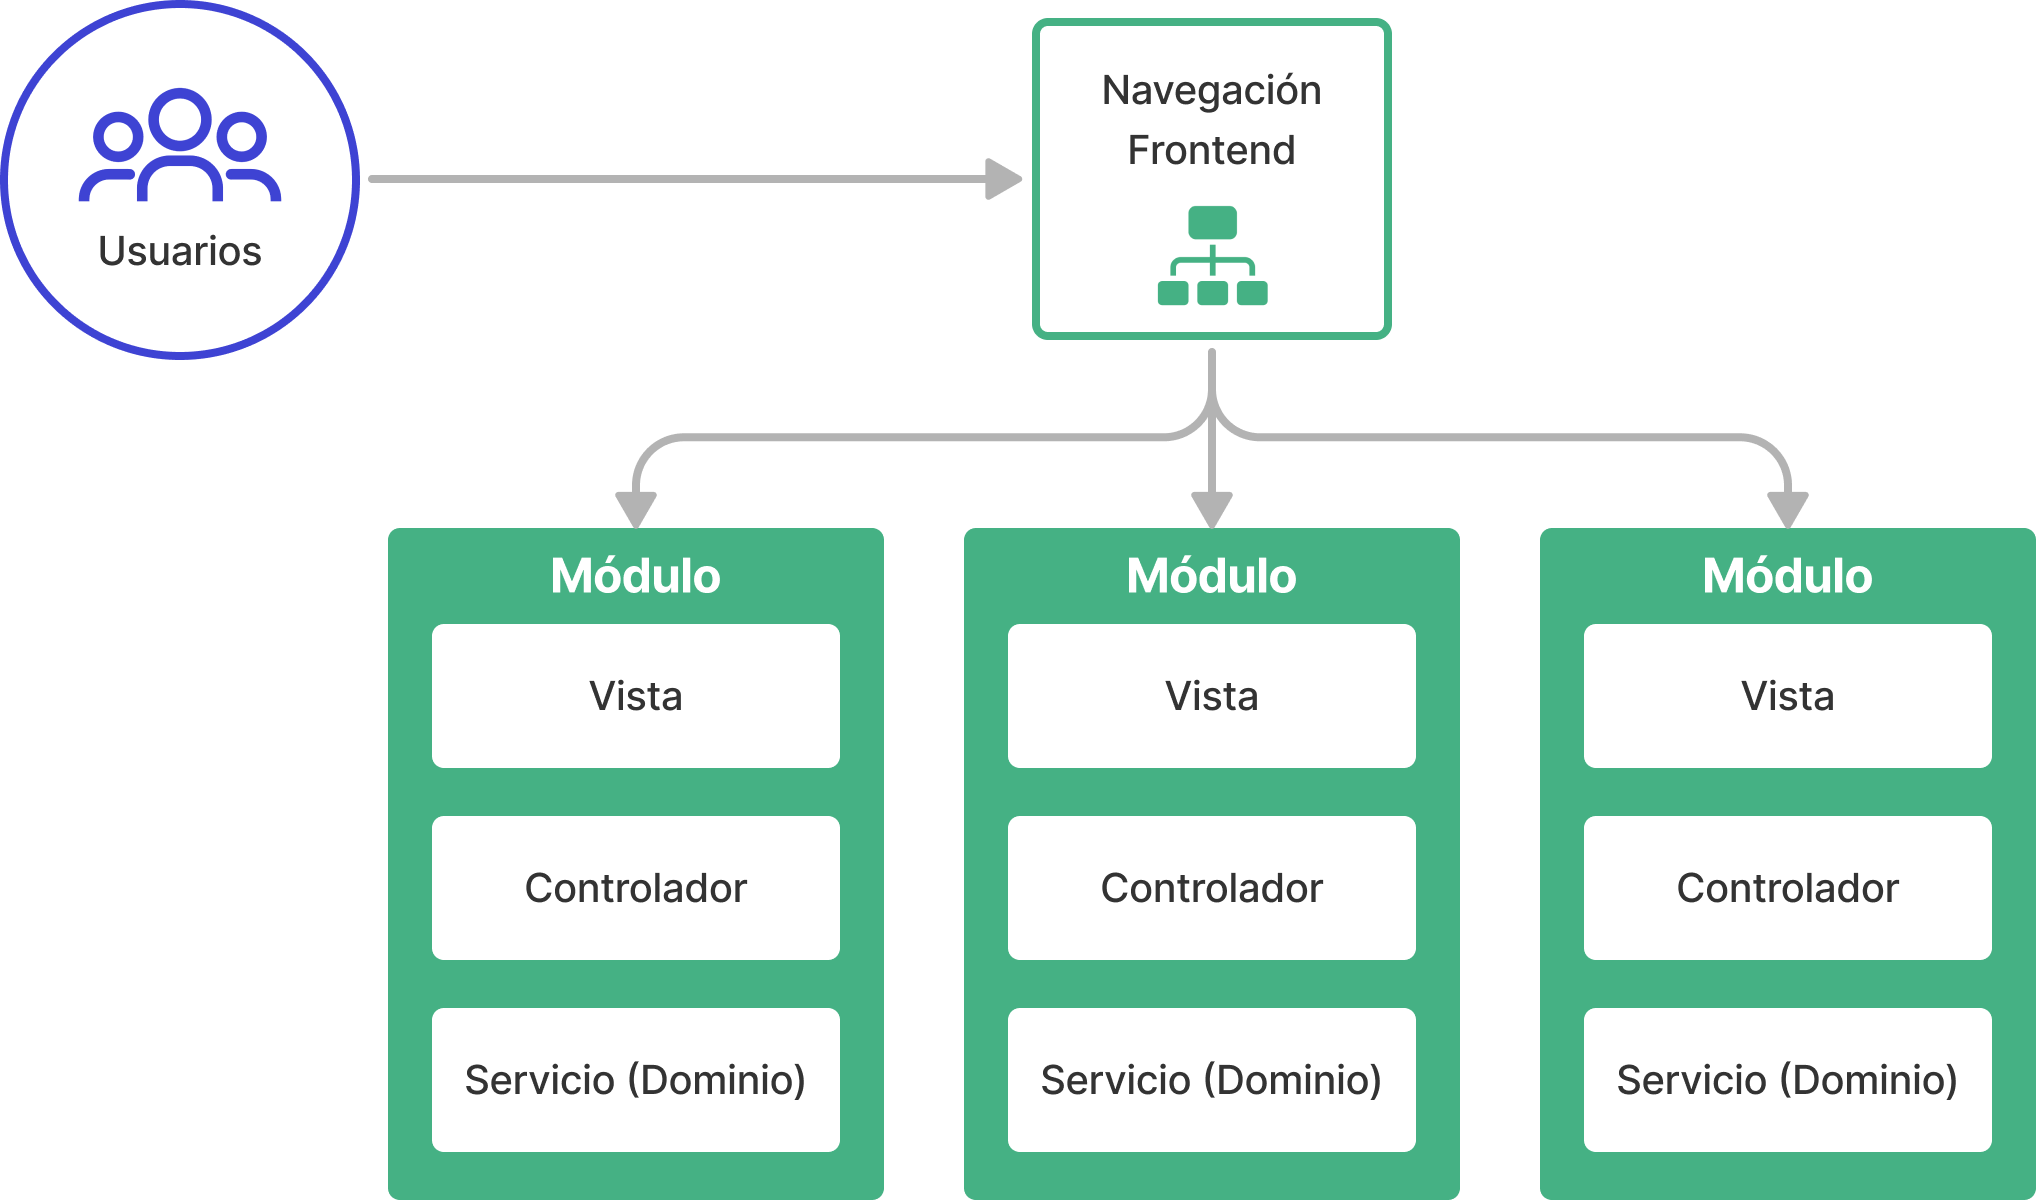
\includegraphics[width=0.8\textwidth]{Figures/frontend-architecture.png}
\caption{Arquitectura de módulos \textit{\gls{frontend}}}
\label{fig:frontend-architecture}
\end{figure}

Para la estructuración interna del código, se eligió implementar una arquitectura Modelo Vista-Controlador (\gls{mvc}), que establece una clara separación de responsabilidades: la vista implementa la interfaz de usuario, el controlador maneja la lógica y las interacciones, y el modelo (en este caso, un servicio) se comunica con el \textit{\gls{backend}}. Esta metodología, combinada con la arquitectura de componentes, facilita una construcción rápida y consistente de cada vista, al mismo tiempo que mejora la mantenibilidad del código a largo plazo, ya que cada componente puede ser actualizado sin afectar otras partes del sistema. En la Figura \ref{fig:frontend-architecture} se ilustra la arquitectura de componentes y módulos del \textit{frontend}, donde los usuarios navegan por las distintas vistas de la aplicación y cada una está compuesta por un módulo con un componente de vista, un controlador que implementa la lógica y un servicio que actúa como modelo, el cual se encarga de enviar solicitudes a la \gls{api} \textit{backend} para interactuar con los datos.

\begin{figure}[!b]
    \centering
    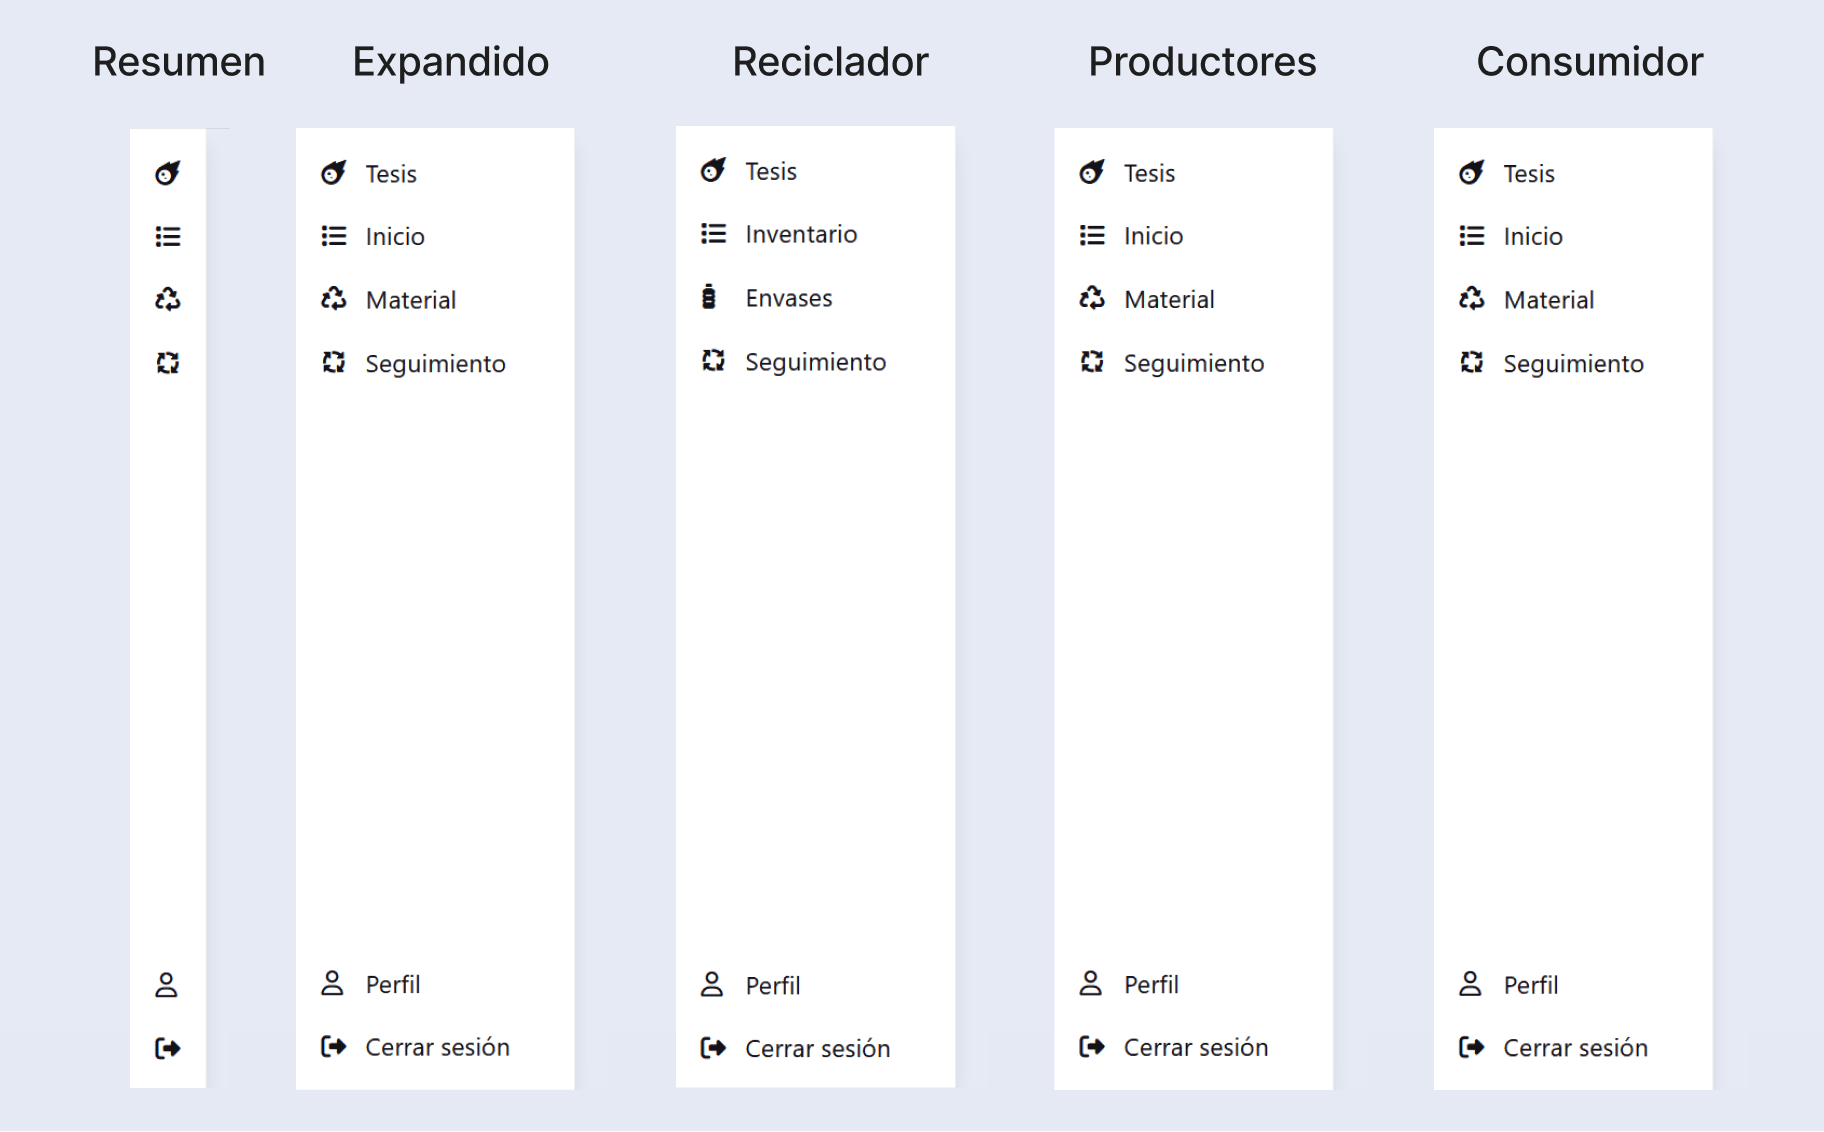
\includegraphics[width=\textwidth]{Figures/frontend-navigation.png}
    \caption{Diseño de casos de la barra lateral de navegación de la aplicación para cada rol}
    \label{fig:frontend-navigation}
\end{figure}

La estructura de la interfaz de usuario se organizó en módulos funcionales por cada rol de usuario, lo cual se alinea con la división de responsabilidades del diseño de arquitectura de \textit{backend} y capa de datos. Por ejemplo, se definieron vistas específicas para el registro y la gestión de lotes por parte de los productores, junto con una interfaz de consulta para los consumidores. En la Figura \ref{fig:frontend-navigation} se puede observar el diseño de la navegación de la aplicación, que consiste en una barra lateral comprimida que se expande al posicionar el cursor sobre ella, mostrando accesos directos a las pantallas disponibles según el rol del usuario autenticado. El contenido de la barra lateral varía dinámicamente según el rol del usuario autenticado para permitir un acceso rápido a las funcionalidades relevantes para cada tipo de usuario. En el Apéndice \ref{cp:user-flows} se encuentran documentados los flujos de usuario para cada rol con imágenes de sus respectivas pantallas y las acciones que conectan el flujo.

\begin{figure}[!t]
    \centering
    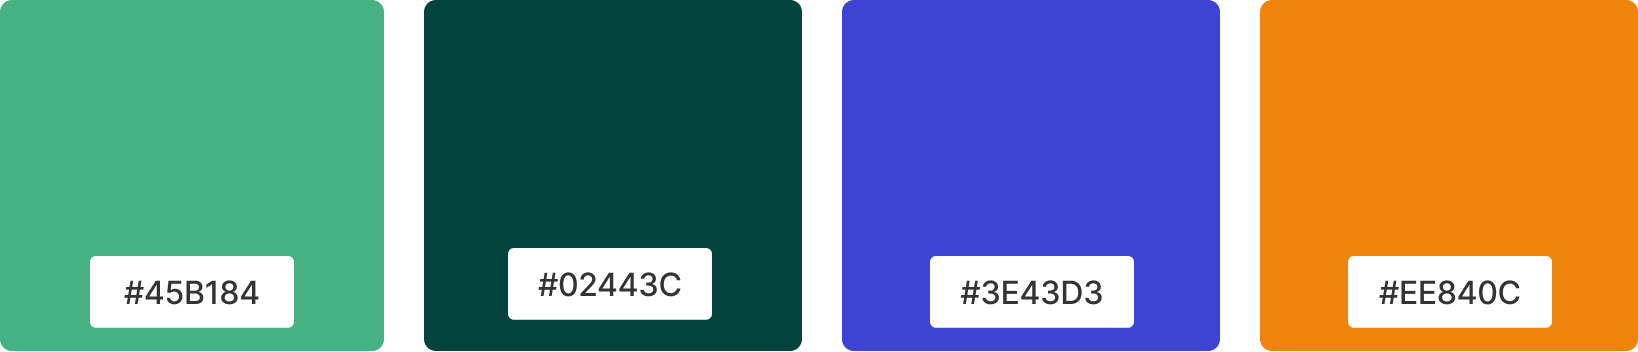
\includegraphics[width=0.8\textwidth]{Figures/frontend-palette.png}
    \caption{Identidad de marca de la aplicación}
    \label{fig:frontend-brand}
\end{figure}

Por otro lado, para asegurar una identidad visual consistente en la aplicación, se definió un sistema de diseño con una paleta de colores basada en tonalidades de verde con el objetivo de transmitir el compromiso ambiental del proyecto mediante la economía circular, así como también tipografías e iconografía que complementan esta estética. En la Figura \ref{fig:frontend-brand} se puede observar una muestra de la identidad de marca de la aplicación, a través de su paleta de colores, que posee un color primario (verde), un color secundario (verde oscuro) y colores complementarios (azul y anaranjado) para resaltar elementos importantes en la interfaz.

Con la definición de las especificaciones detalladas de la arquitectura de componentes para el \textit{frontend}, el \textit{backend} y la capa de datos, el proceso de desarrollo posterior puede ser más fluido, organizado y predecible. En el siguiente capítulo se abordará el proceso de implementación del prototipo tecnológico, a través del cual se materializarán los diseños aquí descritos en un software funcional que cumpla con los requerimientos establecidos.

\chapter[Implementación]{Implementación}
\label{cp:implementation}

\parindent0pt

La fase de implementación representa el proceso de traducción del diseño de software a código ejecutable, constituyendo el puente entre la teoría y la práctica. En el marco del modelo en V, este proceso es una de las etapas finales de la fase descendente, que a su vez marca el inicio de la fase ascendente, ya que la implementación de cada módulo va acompañada de la ejecución de pruebas unitarias. Este enfoque iterativo de desarrollo y validación temprana busca asegurar que la funcionalidad de cada componente se verifique de forma continua para minimizar la aparición de errores cuando el software se despliegue en un entorno real.

La implementación del software se llevó a cabo siguiendo la planificación elaborada a partir de las historias de usuario junto con el diseño del sistema. Durante la ejecución de esta etapa, se utilizó la herramienta Jira para gestionar las tareas en curso y el progreso del desarrollo. El cronograma original enfrentó desviaciones debido a la superposición de actividades académicas y compromisos imprevistos, pero la flexibilidad en la gestión del proyecto permitió la adaptación, posibilitando el cumplimiento de los objetivos del trabajo. En esta fase de desarrollo, se implementa e integra cada uno de los módulos definidos en el proceso de diseño, asegurando su funcionamiento de forma aislada y en conjunto.

El proceso de desarrollo se estructuró para seguir un flujo de trabajo lógico. En primer lugar, se crearon los contratos inteligentes, que conforman la capa más interna del prototipo y definen la lógica de las transacciones en la blockchain. Posteriormente, se construyó la API, que actúa como intermediario para interactuar con los contratos. Finalmente, se desarrolló la interfaz de usuario, que sirve como la capa de presentación. Este enfoque se adoptó con el objetivo de garantizar que cada componente estuviera operativo y probado antes de proceder a la siguiente capa que interactúa con él. A nivel de dominio, el desarrollo siguió secuencialmente el ciclo de vida del vidrio (productor primario, secundario, consumidor, reciclador) para mantener la coherencia del sistema. En la siguiente sección se detalla el proceso de generación de código llevado a cabo durante la implementación del prototipo (Sección \ref{sec:code-generation}). Posteriormente, se describe el proceso de despliegue en un entorno de pruebas (Sección \ref{sec:deployment}). Finalmente, se aborda la estrategia de documentación del software desarrollado (Sección \ref{sec:documentation}).
	
\section{Generación de Código}
\label{sec:code-generation}

La implementación del prototipo se realizó en un entorno de desarrollo local, siguiendo un flujo de trabajo que priorizó la separación por capas para gestionar las dependencias del sistema. Como la lógica de negocio central recae en los contratos inteligentes, su implementación fue la primera en abordarse. La capa de datos no solo define la lógica de las transacciones en la blockchain, sino que también establece el modelo de datos base que utilizan las capas superiores. Una vez que los contratos estuvieron completamente desarrollados y probados en base a las especificaciones de requerimientos y diseño, se procedió a la construcción de la API. Esta capa actúa como un intermediario entre los contratos y el frontend, siendo responsable de traducir las peticiones de la interfaz de usuario en transacciones y llamadas a los contratos. Finalmente, se construyó la interfaz de usuario, que se conecta a la API para poder presentar la información al usuario y permitir la interacción con el sistema.

El proceso de desarrollo se concibió de manera iterativa, donde la escritura de código se alternó con la creación de pruebas unitarias. Este método permitió verificar el correcto funcionamiento de cada componente de forma individual, asegurando que las funciones y módulos cumplieran con las especificaciones de diseño. Gracias al diseño de sistema realizado previamente, la implementación de cada módulo se llevó a cabo de manera sistemática sin bloqueos, pero esto no implicó que no surgieran desafíos técnicos durante la integración de los componentes. Un ejemplo destacable durante la implementación fue el desafío de adaptar la API a la naturaleza inherente de los contratos inteligentes, los cuales no retornan datos de forma nativa, sino que emiten eventos notificando cambios en su estado. Esta particularidad técnica de la blockchain requirió que la capa de la API fuera adaptada para escuchar estos eventos, capturando información como los identificadores únicos de los lotes de vidrio recién creados para su posterior almacenamiento en la base de datos relacional. Esta solución técnica permitió demostrar la viabilidad de la arquitectura híbrida propuesta, asegurando la sincronización de la información entre la blockchain y la base de datos complementaria.

A nivel de dominio, la implementación de las funcionalidades siguió el ciclo de vida del vidrio para mantener una mayor coherencia. El desarrollo se inició con las funcionalidades del productor primario, continuó con las del productor secundario, luego con las del consumidor y, finalmente, con las del centro de reciclaje, cerrando así el ciclo de trazabilidad. Una vez que se completaron las funcionalidades para cada actor, se desarrolló la funcionalidad de seguimiento de extremo a extremo, que permite visualizar el historial completo de un envase desde su producción hasta su revalorización. Este enfoque permitió que el flujo del proceso de trazabilidad se construyera de manera lógica y progresiva. Una vez que todas las funcionalidades del prototipo fueron implementadas a nivel de código, se procedió a realizar el despliegue del prototipo en un entorno de pruebas, como se detalla en la siguiente sección.

\section{Despliegue}
\label{sec:deployment}

Una vez que cada módulo del sistema fue implementado y verificado con pruebas unitarias en un entorno local, se procedió a la fase de despliegue en un entorno de pruebas de características similares a un entorno productivo real. El objetivo principal de esta acción fue demostrar la operatividad del prototipo y simular su funcionamiento en un contexto accesible públicamente. Para ello, se eligieron plataformas gratuitas que permitieran la exposición pública de los componentes del sistema, lo cual facilitó la validación por parte de terceros y la demostración de la viabilidad del proyecto dentro del alcance de un trabajo académico.

En primer lugar, para la modularización y gestión del despliegue, se configuraron contenedores de Docker para cada uno de los componentes del sistema. El uso de esta tecnología permitió empaquetar la aplicación y sus dependencias en unidades portables y autónomas, para poder garantizar la reproducibilidad del trabajo en cualquier entorno y facilitar la futura transición del prototipo a un entorno productivo evitando problemas de compatibilidad debido a diferencias en la configuración del entorno.
Posteriormente, el despliegue se llevó a cabo de forma diferente para cada tecnología. La API de backend se desplegó en una plataforma de alojamiento web \footnote{https://cloud.google.com/}, los contratos inteligentes se publicaron en una red de pruebas de Ethereum \footnote{https://sepolia-optimism.etherscan.io/} y la interfaz de usuario se puso a disposición en un servicio de hospedaje web estático \footnote{https://vercel.com/}. Esta configuración no solo logró que el prototipo fuera accesible en línea, sino que también permitió la ejecución de pruebas de integración y aceptación de usuarios en un entorno que replicaba las condiciones de uso finales. Si bien el prototipo se implementó en un entorno de pruebas, fue diseñado con una arquitectura escalable, con el objetivo de facilitar una transición sin fricciones a un entorno productivo en el futuro.

Finalmente, todos los detalles del proceso de despliegue, incluyendo las instrucciones para la configuración del entorno local y la replicación del despliegue en producción, se documentaron exhaustivamente en cada repositorio del proyecto. Esta documentación asegura que otros desarrolladores o investigadores puedan reproducir el entorno de desarrollo y desplegar el sistema de manera autónoma, contribuyendo a la transparencia y accesibilidad del trabajo realizado. En la siguiente sección se detalla la estrategia de documentación adoptada para el prototipo desarrollado.

\section{Documentación}
\label{sec:documentation}

Como parte integral del proceso de ingeniería de software, la documentación busca asegurar la mantenibilidad del código, facilitar la colaboración futura y consolidar el conocimiento técnico del proyecto. En este trabajo, el prototipo se documentó en tres niveles: la documentación del código fuente, la interfaz de la API y la configuración del proyecto.

En el primer nivel, se incluyeron comentarios directamente en el código fuente de cada repositorio, tanto en los contratos inteligentes, como en la API y el frontend. Esto permite que el código sea autoexplicativo y más fácil de comprender para otros desarrolladores o para futuros trabajos de mantenimiento. En el segundo nivel, se utilizó la especificación de OpenAPI para describir la interfaz de la API del backend, detallando todos los endpoints, parámetros y formatos de solicitudes y respuestas. A partir de este estándar, se utilizó una librería para generar un sitio web interactivo que presenta esta documentación de manera accesible. Exponer esta documentación facilita que la API sea interoperable y pueda ser consumida por cualquier otra aplicación cliente, por ejemplo, en el caso de que se desarrollen nuevas interfaces de usuario o aplicaciones móviles que se conecten a la misma API.

Finalmente, en el tercer nivel, cada repositorio cuenta con un archivo \textit{README} que actúa como una guía de referencia rápida para la configuración y operación del sistema. Estos archivos detallan los requisitos técnicos, la estructura del proyecto y los comandos para ejecutar pruebas y desplegar el sistema. A su vez, también se incluyó una explicación de la arquitectura de cada repositorio y una serie de enlaces de utilidad que pueden ser de ayuda para los desarrolladores que comiencen a interactuar con el código del proyecto.

Concluido el proceso de implementación y documentación, el prototipo del sistema de trazabilidad del vidrio se considera listo para la fase de validación. La construcción de cada componente, desde los contratos inteligentes hasta la interfaz de usuario, ha sido exhaustivamente verificada con pruebas unitarias, sentando las bases para una evaluación más rigurosa. El siguiente capítulo, ``Pruebas``, abordará en detalle este proceso de verificación, detallando la metodología de pruebas unitarias, de integración, de sistema y de aceptación del usuario para asegurar la calidad y el correcto funcionamiento del prototipo en su conjunto.

\chapter[Pruebas]{Pruebas}
\label{cp:testing}

\parindent0pt

El presente capítulo aborda el proceso de pruebas del prototipo, un componente central del Modelo en V de ingeniería de software que rige el desarrollo de este trabajo. Este proceso de validación, que abarca la totalidad de la segunda mitad del modelo, tiene como objetivo principal verificar que el prototipo se alinee con los requerimientos y el diseño definidos en las fases previas. El proceso de pruebas se estructura en un ciclo progresivo, donde la granularidad de la validación disminuye a medida que se avanza en las etapas, comenzando por las unidades de código más pequeñas y atómicas (pruebas unitarias), avanzando con pruebas de integración entre los módulos del sistema, hasta alcanzar la validación del sistema en su totalidad (pruebas de sistema y de aceptación). La naturaleza de estas pruebas varía entre automatizada y manual. Las pruebas automatizadas, si bien requieren una inversión inicial, se ejecutan de manera instantánea y repetible, lo cual resulta ideal para verificar comportamientos de forma constante. Por su parte, las pruebas manuales, aunque resultan más lentas de ejecutar, permiten una validación completa de los flujos de usuario y la experiencia general del sistema.

A continuación, se detallan las cuatro etapas de pruebas integrales realizadas en el proyecto:

\begin{itemize}
\item Pruebas Unitarias: se enfocan en la validación del código a nivel de componente.
\item Pruebas de Integración: verifican la interacción entre los módulos del sistema.
\item Pruebas de Sistema: validan el cumplimiento de los requerimientos funcionales y no funcionales del prototipo en su totalidad.
\item Pruebas de Aceptación con Usuarios: validan que el prototipo cumpla con las expectativas y necesidades del usuario final.
\end{itemize}
La Tabla \ref{tab:testing-comparison} presenta una comparación de estas etapas, destacando sus características y su alcance, como una guía visual para comprender la metodología de prueba aplicada.

\begin{xltabular}{\textwidth}{@{} L{4cm} Y L{2cm} L{2cm} L{3cm} @{}}
	\caption{Comparación de las etapas de prueba del prototipo de trazabilidad de vidrio}
	\label{tab:testing-comparison}\\
	\toprule
	Etapa de Prueba & Frec. Ejecución & Tipo & Complejidad & Alcance \\
	\midrule
\endfirsthead

\toprule
Etapa de Prueba & Frec. Ejecución & Tipo & Complejidad & Alcance \\
\midrule
\endhead

\midrule
\multicolumn{5}{r}{\footnotesize Continúa en la siguiente página}
\\\bottomrule
\endfoot

\bottomrule
\endlastfoot

Pruebas Unitarias & Continua (por cada cambio) & Automatizada & Baja & Componentes \\
Pruebas de Integración & Antes de cada despliegue & Automatizada & Media & Interacción de componentes \\
Pruebas de Sistema & Al finalizar la implementación & Manual & Media-Alta & Requerimientos funcionales \\
Pruebas de Aceptación & Al finalizar la implementación & Manual & Alta & Experiencia del usuario \\

\end{xltabular}

A lo largo de este capítulo, se detallará la gestión de las incidencias halladas durante las pruebas. Los errores detectados en cada etapa de prueba fueron registrados y se les dio seguimiento en la herramienta Jira, asegurando que cada problema se resolviera antes de avanzar a la siguiente fase. El Apéndice \ref{cp:tests-execution-results} contiene los detalles de la ejecución de cada prueba, los resultados obtenidos y la gestión de las incidencias documentadas. A continuación, se describen en detalle cada una de las etapas de prueba mencionadas, proporcionando una visión completa del proceso de validación del prototipo.

\section{Pruebas Unitarias}
\label{sec:unit-testing}

Las pruebas unitarias constituyen la base de la pirámide de pruebas y se corresponden directamente con la fase de codificación del Modelo en V. Su objetivo es validar la unidad más pequeña de código de forma aislada del resto del sistema, por ejemplo, un método de un contrato inteligente, un endpoint de backend o un componente reutilizable del frontend. La naturaleza atómica de estas pruebas permite verificar que cada componente individual se comporte de acuerdo con las especificaciones de diseño antes de ser integrado con otras partes del prototipo. Para este proyecto, se implementaron pruebas unitarias automatizadas para permitir una verificación continua de la integridad del código a lo largo de todo el proceso de implementación y luego de cada modificación de código posterior.

El desarrollo de cada módulo del prototipo se realizó de forma conjunta con la escritura de sus pruebas unitarias. Se utilizó el framework Jest \footnote{https://jestjs.io/} en las tres capas del proyecto (contratos inteligentes, API y frontend), aunque con configuraciones específicas para cada entorno. Por ejemplo, en los contratos inteligentes, las pruebas unitarias se orientaron a verificar que la lógica de negocio se ejecute correctamente y que el estado de los contratos cambie como se espera. En el backend, se enfocaron en validar la lógica de negocios. En el frontend, se validó el comportamiento de los componentes, su estado interno y la interacción con la API.

Un indicador representativo de la calidad de las pruebas unitarias es la cobertura de código (conocida comúnmente como \textit{coverage}), que mide el porcentaje de código fuente ejecutado por las pruebas. Este valor, si bien no garantiza la ausencia de errores, es una herramienta útil para evaluar la robustez del código. Los requisitos de cobertura mínima se definieron en función de la criticidad de cada módulo del sistema:

\begin{itemize}
\item Contratos Inteligentes: se requirió una cobertura mínima del 100\%. Dado que los contratos son la base del sistema de trazabilidad y no pueden modificarse una vez desplegados, resulta fundamental garantizar que todos los caminos de ejecución del código estén cubiertos para minimizar el riesgo de errores una vez desplegados. Este es un estándar de la industria para contratos inteligentes.
\item API Backend: se requirió una cobertura mínima del 80\%. Dado que la API representa el componente central del sistema como responsable de la comunicación con la blockchain y la base de datos, resulta relevante garantizar la calidad del código y minimizar el riesgo de errores en el manejo de datos. Por este motivo, se ha elegido este umbral de cobertura, que es un estándar habitual en la industria para aplicaciones de propósito general.
\item Aplicación Frontend: se estableció una cobertura mínima del 60\%. Dado que el frontend del prototipo tiene fines demostrativos y no es una parte crítica del sistema, este umbral se consideró suficiente para garantizar el correcto funcionamiento de la interfaz de usuario sin requerir un esfuerzo excesivo en la escritura de pruebas.
\end{itemize}

El proceso de pruebas unitarias permitió identificar y corregir algunos errores de manera temprana. Los errores detectados en esta etapa fueron resueltos de manera inmediata, ya que las pruebas unitarias son cercanas a la implementación y permiten una rápida retroalimentación sobre el estado del código. En la Tabla \ref{tab:unit-testing-summary} se muestra un resumen de las pruebas unitarias realizadas, mientras que en el Apéndice \ref{cp:tests-execution-results} se puede consultar en mayor detalle el listado de casos de prueba.

% TODO: Replace all tables that are not xltabular

\begin{table}[!htb]
\centering
\caption{Resumen de Pruebas Unitarias}
\label{tab:unit-testing-summary}
\begin{tabular}{|l|c|c|c|}
\hline
\textbf{Módulo} & \textbf{Coverage Objetivo} & \textbf{Coverage Alcanzado} & \textbf{Cant. de Pruebas} \\
\hline
Contratos Inteligentes & 100\% & 100\% & 98 \\
API Backend & 80\% & 90.84\% & 317 \\
Aplicación Frontend & 60\% & 65.27\% & 286 \\
\hline
\end{tabular}
\end{table}

La ejecución automatizada de las pruebas unitarias proporciona una capa de seguridad que facilita la revalidación del comportamiento del sistema, lo cual es relevante en un prototipo que podría expandirse en un futuro. La validación constante de la base de código antes de cualquier despliegue favorece la estabilidad y la calidad del sistema a largo plazo. Una vez que se ha verificado el funcionamiento de cada componente del sistema de forma individual, es posible continuar con la siguiente etapa de validación, donde se verificará la correcta interacción entre los módulos del sistema.

\section{Pruebas de Integración}
\label{sec:integration-testing}

Las pruebas de integración se sitúan en la siguiente capa de la pirámide de pruebas. Su objetivo principal consiste en verificar que los distintos componentes y módulos del sistema interactúen correctamente y de forma coherente con sus responsabilidades. A diferencia de las pruebas unitarias, que validan el funcionamiento aislado de una unidad de código, las pruebas de integración evalúan el flujo de datos y las interacciones entre componentes para asegurar que sus interfaces y responsabilidades estén debidamente sincronizadas. Esta etapa de prueba se corresponde con la fase de diseño de componentes del Modelo en V, donde se definen las interacciones entre los módulos del sistema.

Para este proyecto, las pruebas de integración se diseñaron para ser automatizadas y se enfocaron en los puntos de interacción más críticos del sistema. El entorno de prueba se configuró para simular un escenario lo más cercano posible a un entorno real, pero aislado, sin hacer uso de funcionalidades simuladas. Por ejemplo, mientras que durante las pruebas unitarias se simularon los datos que debería retornar la blockchain para probar la funcionalidad de la API, durante las pruebas de integración se utilizaron datos reales obtenidos de un entorno virtual de la red blockchain. De esta manera, se pudo validar que la comunicación entre los módulos funciona correctamente en un contexto más realista.

El proceso de pruebas de integración no detectó fallos en la interacción entre los módulos. Se realizaron pruebas de integración para 18 casos de uso del sistema, los cuales se han documentado en el Apéndice \ref{cp:tests-execution-results}. La ejecución de estas pruebas proporciona una capa de verificación adicional del sistema y se recomienda ejecutarlas de forma rutinaria antes de cada despliegue en un entorno productivo para mitigar los riesgos asociados a los cambios en el código que puedan afectar la interacción entre los módulos del sistema. Una vez que se ha validado la interacción de los componentes, la siguiente etapa consiste en verificar que el sistema en su totalidad cumpla con los requisitos funcionales y no funcionales definidos al comenzar el proyecto.

\section{Pruebas de Sistema}
\label{sec:system-testing}

Las pruebas de sistema constituyen la siguiente fase en el ciclo de validación y tienen como propósito verificar que el prototipo, en su conjunto, cumple con los requerimientos funcionales y no funcionales definidos al comenzar el proyecto. Esta etapa se corresponde con el diseño de arquitectura en el Modelo en V, y su objetivo es evaluar el comportamiento del sistema de manera integral para asegurar que la arquitectura implementada efectivamente logra cumplir los requisitos establecidos.

A diferencia de las pruebas unitarias y de integración, que fueron automatizadas, las pruebas de sistema se ejecutaron de manera manual. En primer lugar, se documentó de forma detallada cada caso de prueba a ejecutarse, incluyendo un título, requerimientos asociados, los pasos a seguir desde la perspectiva de un usuario, los datos de entrada (en caso de requerirlos) y los resultados esperados. Posteriormente, se ejecutó de forma manual cada caso de prueba, siguiendo los pasos definidos y registrando los resultados obtenidos. La metodología consistió en interactuar con la interfaz de usuario (frontend) del sistema y seguir los pasos detallados en el caso. En estas pruebas, se utilizó el sistema completo desplegado en el entorno de pruebas, sin emplear datos simulados ni probar funcionalidades de forma aislada. Esto permitió una validación precisa del comportamiento del prototipo, desde la perspectiva de un usuario, en un entorno que replicaba la realidad.

A su vez, también se incluyeron pruebas de requerimientos no funcionales en esta etapa, como son la escalabilidad, el rendimiento y la seguridad del sistema. A pesar de las limitaciones de recursos del entorno de pruebas (debido a que se utilizaron plataformas gratuitas), se llevaron a cabo pruebas controladas para validar que el sistema puede cumplir con estos requerimientos en un entorno real. Los detalles y resultados de estas pruebas se documentaron junto con los casos de prueba funcionales en el Apéndice \ref{cp:tests-execution-results}.

El proceso de pruebas de sistema incluyó un total de 55 casos de prueba y resultó en la identificación de 7 incidencias, las cuales fueron registradas y rastreadas en la herramienta Jira hasta su resolución. La ejecución de estas pruebas permitió identificar y corregir errores, pero también puede servir como una base para futuras pruebas de regresión del sistema, ayudando a prevenir que cualquier cambio o nueva funcionalidad no afecte negativamente el comportamiento actual. Luego de esta etapa, el prototipo ya está listo para ser presentado a un grupo reducido de usuarios, quienes serán responsables de evaluar su funcionalidad durante las pruebas de aceptación.

\section{Pruebas de Aceptación con Usuarios}
\label{sec:user-acceptance-testing}

La fase final de validación del prototipo corresponde a las Pruebas de Aceptación con Usuarios (\textit{UAT}, por sus siglas en inglés). Esta etapa se enfoca en verificar que el sistema no solo funcione correctamente a nivel técnico, sino que también satisfaga las necesidades y expectativas del usuario final, tal como se definieron en la etapa de modelado de requerimientos del Modelo en V. En esta instancia, un grupo reducido de usuarios es convocado para utilizar el sistema en un entorno controlado, de forma similar a cómo utilizaría el sistema en su rutina habitual. 

Dada la naturaleza de este trabajo como proyecto académico, la obtención de usuarios reales de la industria del vidrio para la ejecución de estas pruebas presentó una limitación. No obstante, se llevó a cabo un experimento controlado con un grupo de usuarios voluntarios del entorno académico. El experimento se realizó en un laboratorio de computación, donde cada usuario voluntario contó con una computadora de escritorio con acceso a Internet, desde donde pudo acceder al frontend del prototipo desplegado en el entorno de pruebas. La metodología de la prueba combinó una fase guiada y una fase libre, creando un entorno mixto, donde los participantes recibieron una guía para ejecutar una serie de casos de prueba predefinidos, seguidos de un período de exploración libre del sistema. Este enfoque permitió validar tanto los flujos de trabajo específicos como la usabilidad general del prototipo. Los participantes evaluaron tanto los requerimientos funcionales (por ejemplo, la capacidad de registrar un lote de vidrio) como los no funcionales (como la facilidad de uso y la transparencia de la información) registrando en una planilla la descripción del caso de prueba ejecutado y el resultado obtenido.

La ejecución de las pruebas generó una retroalimentación detallada que se utilizó para identificar y resolver fallos, así como para mejorar la experiencia de usuario (UX) y el diseño de la interfaz. Se registraron en Jira un total de 9 incidencias y 3 sugerencias recibidas para su posterior seguimiento. Como resultado directo de estas pruebas, se realizaron mejoras en los flujos de navegación, la presentación de los datos de trazabilidad y el diseño visual de la aplicación. En el Apéndice \ref{cp:tests-execution-results} se encuentran documentados los casos de prueba ejecutados durante el experimento y la retroalimentación de los participantes. En las Figuras \ref{fig:uat-picture-1} y \ref{fig:uat-picture-2} se pueden observar fotografías tomadas durante la ejecución del experimento, donde se puede observar a los usuarios voluntarios del experimento utilizando el prototipo.

\begin{figure}[!htb]
\centering
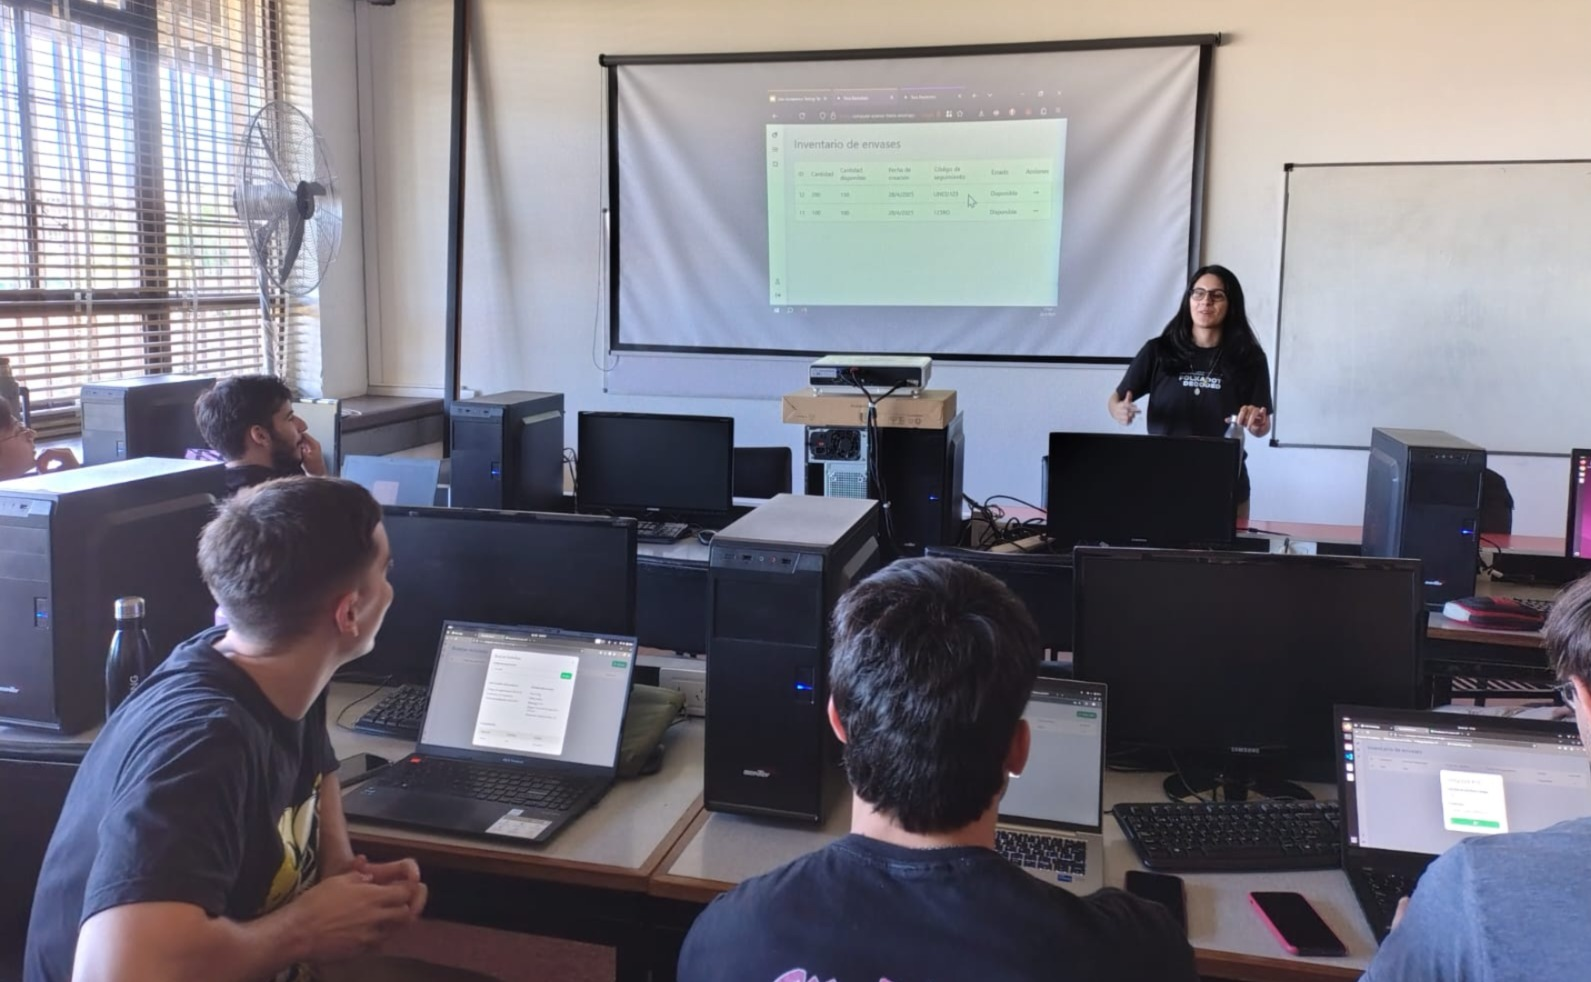
\includegraphics[width=0.8\textwidth]{Figures/uat-1.jpg}
\caption{Usuarios interactuando con el prototipo durante prueba guiada}
\label{fig:uat-picture-1}
\end{figure}

\begin{figure}[!htb]
\centering
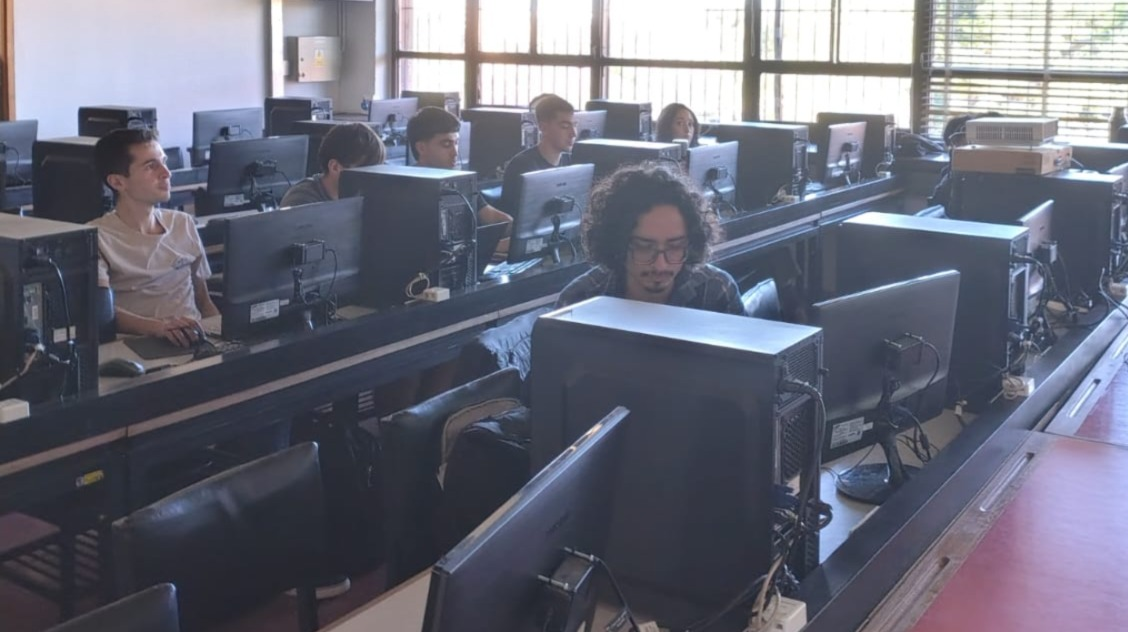
\includegraphics[width=0.8\textwidth]{Figures/uat-2.jpg}
\caption{Usuarios voluntarios durante el experimento}
\label{fig:uat-picture-2}
\end{figure}

Al finalizar la etapa de pruebas con usuarios, se llevó a cabo una revisión de los resultados obtenidos. El riguroso proceso de pruebas llevado a cabo, desde las unidades más pequeñas de código hasta la validación con usuarios voluntarios, demostró que el prototipo desarrollado es funcional y está alineado con los requerimientos originales del proyecto. Esta etapa de validación confirma la viabilidad del sistema de trazabilidad del vidrio basado en blockchain, estableciendo un precedente sólido para su potencial escalabilidad y aplicación en un entorno productivo. La finalización de esta fase marca la conclusión del ciclo de vida del desarrollo del software de este proyecto académico, cuyos principales hallazgos, lecciones aprendidas y oportunidades de mejora se resumen en el siguiente capítulo.


%%% Conclusiones %%%

\chapter[Conclusiones]{Conclusiones}
\label{cp:conclusions}

\parindent0pt

En este capítulo de conclusiones, tras haber validado técnicamente el prototipo mediante pruebas rigurosas, se presentan las conclusiones generales del trabajo realizado. Adicionalmente, se reflexiona sobre el proceso de desarrollo del prototipo de trazabilidad de envases de vidrio, analizando los resultados obtenidos, los desafíos superados y las perspectivas futuras que emanan de este trabajo. Se busca ofrecer una visión completa que no solo se limite a lo técnico, sino que también abarque la experiencia metodológica y el potencial de impacto real de la solución.

\section{Conclusiones del trabajo}

En este trabajo se desarrolló un prototipo tecnológico que implementa un sistema de trazabilidad para envases de vidrio en la industria vitivinícola, utilizando tecnología \textit{blockchain}. El objetivo principal fue diseñar e implementar una solución que permita rastrear el ciclo de vida de los envases desde su producción hasta su reciclaje, con el fin de garantizar el cumplimiento normativo, mejorar la eficiencia operativa, fomentar la sostenibilidad y aumentar la confianza entre todos los actores involucrados en el proceso. El resultado final del trabajo fue un prototipo tecnológico funcional con una interfaz de usuario cuidada y una experiencia de usuario validada a través de un riguroso proceso de pruebas. A partir de los resultados obtenidos, se concluye que los objetivos planteados fueron cumplidos satisfactoriamente y que este prototipo representa una prueba de concepto que demuestra la viabilidad del uso de tecnología \textit{blockchain} para impulsar la transparencia y la sostenibilidad en la industria vitivinícola de la región.

Al reflexionar sobre el proceso de ejecución de este trabajo y los resultados obtenidos, se considera que la elección del modelo en V para guiar el desarrollo del prototipo fue idónea. Esta metodología, que se asocia habitualmente a proyectos de gran escala que demandan alta calidad, demostró ser altamente eficaz en este contexto. La inmutabilidad de la tecnología \textit{blockchain} (y de los contratos inteligentes) exige un enfoque que minimice la aparición de errores en las etapas finales del ciclo de vida del software. En este sentido, las fases de definición de requerimientos y diseño del software previo a su implementación, así como la ejecución de pruebas unitarias desde la implementación, propuestas por el modelo en V fueron valiosas, permitiendo detectar y corregir inconsistencias de diseño e integración antes de la implementación, lo que facilitó un desarrollo tanto ágil como robusto.

A pesar de la rigidez de la metodología, el proceso de ejecución se adaptó a las circunstancias. Aunque la planificación inicial se desvió 4 semanas debido a contratiempos, como los viajes o las cargas académicas, no impidieron el avance continuo del proyecto. De hecho, el viaje de investigación a Europa motivado por una iniciativa profesional, aunque desvió el cronograma, enriqueció de forma significativa el proyecto, proporcionando una perspectiva global sobre la economía circular y la cultura del reciclaje. Esta experiencia personal reforzó la convicción sobre la aplicabilidad del trabajo, destacando que la flexibilidad y la resiliencia son también componentes valiosos en la gestión de proyectos académicos, particularmente en entornos de investigación aplicada con restricciones reales de tiempo y recursos. Luego de la retrospectiva, se concluye que este trabajo cumple con los objetivos planteados y se valora positivamente el resultado final, la ejecución de la metodología y los aprendizajes adquiridos.

\section{Reflexiones finales}

El desarrollo de este trabajo no estuvo exento de desafíos, muchos de los cuales fueron tan importantes como el propio desarrollo del código. El primer gran reto fue ir más allá de la dimensión técnica para comprender las motivaciones, necesidades y limitaciones de los distintos actores involucrados en la cadena de valor. Plantear una solución que pudiera atender las particularidades de cada uno, desde el productor hasta el reciclador, requirió una labor de análisis y conceptualización que sentó las bases para el éxito del prototipo.

Desde el punto de vista técnico, la implementación de tecnología \textit{blockchain} sin experiencia previa representó una curva de aprendizaje considerable. A pesar de su complejidad, se constató que \textit{blockchain} es una tecnología altamente pertinente para resolver problemas asociados a transparencia y descentralización. Los aprendizajes adquiridos a lo largo de este proceso de desarrollo son un activo valioso, y la experiencia con \textit{blockchain} abre la puerta a futuras investigaciones y aplicaciones relacionadas.

A nivel metodológico, la adaptación de un proceso pensado para un equipo a un trabajo individual fue otro desafío. El uso de herramientas de gestión de proyectos como Jira fue una estrategia eficaz para mantener el orden, la visibilidad del progreso y la trazabilidad de las tareas, indicando que la disciplina metodológica contribuye al éxito incluso en proyectos unipersonales. Por último, la validación del sistema con usuarios en un contexto académico fue un reto que se abordó con creatividad, recurriendo a usuarios voluntarios para simular un entorno de pruebas realista y obtener una retroalimentación valiosa que permitió refinar la interfaz y la experiencia de usuario.

\section{Perspectivas futuras}

Con una perspectiva a futuro, se estima que este trabajo de grado representa una prueba de concepto con un gran potencial de escalabilidad y expansión. En primer lugar, la arquitectura del sistema puede extenderse para incluir la trazabilidad de otros materiales, como el plástico y el aluminio. Además, el prototipo puede servir como el núcleo que potencie una familia de aplicaciones independientes, desarrolladas a la medida de cada actor de la cadena, o que sirvan como incentivo a los ciudadanos, tal como se observó en múltiples proyectos revisados en el estado del arte. A su vez, la apertura del sistema es una perspectiva relevante a futuro, ya que la trazabilidad podría iniciarse en cualquier punto de la cadena de valor, para reducir la barrera de entrada y facilitar la adopción del sistema.

Desde una perspectiva técnica, las mejoras futuras podrían incluir la integración con sensores \gls{iot} en las líneas de producción para automatizar la carga de información, minimizando el error humano. A nivel de impacto, la implementación de esta solución podría tener una influencia positiva en la cultura de la sostenibilidad en la región. Como se observó en las investigaciones de campo en Europa, la confianza generada por la trazabilidad y la transparencia puede ser una herramienta para generar conciencia ciudadana. Al proveer a los consumidores de información sobre el ciclo de vida de los productos, se puede impulsar un cambio de comportamiento que beneficie a la economía y ecología locales.


%%% Appendices: Work that *YOU* Developed %%%
\appendix
\addtocontents{toc}{\protect\contentsline{chapter}{Apéndices}{}{}}

\ifthenelse{\equal{\MediaOption}{paper}}{\blankpage}{\clearpage}
\begin{center}
    \crimsonfont
    \thispagestyle{empty}
        
    \vspace*{\fill}
    {\LARGE\fontsize{26}{26}\selectfont\textcolor{maincolor}{Apéndices}\par}
    \vspace*{\fill}
\end{center}
\MediaOptionLogicBlank

\chapter{Contenido Anexo}
\label{cp:annex-content}

\parindent0pt

\section{Multimedia}

Como parte de este Trabajo Final se grabó un video resumiendo los puntos más importantes del mismo y mostrando el funcionamiento de la plataforma desarrollada. El mismo se encuentra disponible en el siguiente enlace: [enlace al video] % TODO: add this link.

\section{Código fuente}

Todo el código del prototipo se encuentra disponible y accesible en un repositorio público de GitHub. El mismo puede ser consultado en el siguiente enlace: [enlace al repositorio] % TODO: add this link.

\section{Documentación técnica}

La documentación técnica del sistema se encuentra disponible en el repositorio de GitHub mencionado anteriormente. Esta documentación incluye:
\begin{itemize}
		\item Descripción de la arquitectura del sistema.
		\item Instrucciones de instalación y despliegue.
		\item Guía de uso de la API.
		\item Detalles sobre la implementación de los smart contracts.
		\item Información sobre las pruebas realizadas.
		\item Detalles sobre la configuración del entorno de desarrollo.
\end{itemize}

% TODO: Add more to this and list other developed docs.

\chapter{Tecnologías Blockchain}
\label{cp:blockchain-technologies}

\parindent0pt

% TODO: format and redact this chapter.

La tecnología blockchain es en sí misma un tipo de tecnología, pero a la hora de utilizarla para un caso de uso específico no se implementa desde cero, ya que sería el equivalente a desarrollar un sistema de gestión de bases de datos desde cero para cada proyecto. En cambio, se utilizan plataformas blockchain ya desarrolladas y probadas, que ofrecen una serie de características y funcionalidades que facilitan el desarrollo y la implementación de aplicaciones descentralizadas. Cada una de estas plataformas se denomina \textit{protocolo blockchain} y en existen múltiples protocolos blockchain disponibles y ampliamente utilizados actualmente, cada uno con sus propias características y ventajas.

En la etapa de investigación y diseño de solución de este trabajo se analizó la oferta de protocolos blockchain disponibles y se preseleccionaron cinco tecnologías blockchain líderes en la industria para su análisis y comparación. Estas tecnologías se seleccionaron en función de su relevancia, popularidad y características técnicas, y se evaluaron en función de su idoneidad para el caso de uso específico de trazabilidad en la cadena de suministro del vidrio. 

Las tecnologías seleccionadas fueron: Hyperledger Fabric, Ethereum, Polkadot, VeChain y Cardano. Cada una de estas tecnologías tiene sus propias características, ventajas y desventajas, y fue importante comprender sus diferencias para seleccionar la tecnología más adecuada para este caso de uso específico.

Cada tecnología se compara en distintos aspectos clave relevantes para este trabajo. Como el tipo de tecnología, el protocolo de consenso, el lenguaje de programación, la interoperabilidad, la adopción real y el tamaño de la comunidad. A continuación, se presenta una descripción detallada de cada tecnología y una comparación de sus características.

\section{Hyperledger Fabric}

Hyperledger Fabric es una plataforma de tecnología ledger distribuida (DLT) de código abierto y diseñada para uso en contextos empresariales \footnote{https://hyperledger-fabric.readthedocs.io/en/latest/index.html}. Hyperledger se estableció bajo la Fundación Linux y su sólida comunidad \cite{androulaki2018hyperledger}. 

Fabric tiene una arquitectura altamente modular y configurable, que permite la innovación, la versatilidad y la optimización para una amplia gama de casos de uso de la industria, incluida la cadena de suministro. Esta es la primera plataforma de ledger distribuida que admite contratos inteligentes creados en lenguajes de programación de uso general como Java, Go y Node.js, en lugar de lenguajes específicos de dominio restringidos (DSL). Esto significa que en la mayoría de los casos no requiere capacitación adicional para aprender un nuevo idioma para desarrollo de contratos inteligentes.

La plataforma Fabric también es permisionada, lo que significa que, a diferencia de una red pública sin permiso, los participantes se conocen entre sí, en lugar de ser anónimos y, por lo tanto, no se confía en absoluto. A su vez la plataforma tiene compatibilidad con protocolos de consenso conectables que permiten que la plataforma se personalice de manera más eficaz para adaptarse a casos de uso particulares y modelos de confianza. 

Fabric puede aprovechar los protocolos de consenso que no requieren una criptomoneda nativa para incentivar la minería costosa o impulsar la ejecución de contratos inteligentes. Evitar una criptomoneda reduce algunos vectores de riesgo / ataque significativos, y la ausencia de operaciones de minería criptográfica significa que la plataforma se puede implementar con aproximadamente el mismo costo operativo que cualquier otro sistema distribuido.

La combinación de estas características diferenciadoras de diseño convierte a Fabric en una de las plataformas de mejor rendimiento disponibles en la actualidad tanto en términos de procesamiento de transacciones como de latencia de confirmación de transacciones, y permite privacidad y confidencialidad de transacciones y los contratos inteligentes que los implementan.

\section{Ethereum}

Ethereum es una plataforma de código abierto basada en blockchain que permite a los desarrolladores crear y desplegar contratos inteligentes y aplicaciones descentralizadas (dApps) \footnote{https://ethereum.org/en/learn/}. Ethereum tiene como objetivo ser una computadora mundial descentralizada que ejecute cualquier tipo de aplicación. Esta plataforma es alimentada por su criptomoneda nativa, Ether, que se utiliza para pagar las transacciones y los servicios de la red \cite{buterin2013ethereum}.

Esta plataforma fue pionera en la creación de contratos inteligentes y ha sido un líder en la industria desde su lanzamiento en 2015. Ethereum es una plataforma de blockchain pública y sin permiso, lo que significa que cualquiera puede unirse a la red y participar en la validación de transacciones y la ejecución de contratos inteligentes. 

Los contratos inteligentes en Ethereum se escriben en Solidity \cite{dannen2017introducing}, un lenguaje de programación específico de dominio que se utiliza para definir las reglas y la lógica de una aplicación descentralizada. Los contratos inteligentes en Ethereum se ejecutan en la máquina virtual Ethereum (EVM), que es una máquina virtual Turing completa que puede ejecutar cualquier tipo de código. El lenguaje Solidity está inspirado en JavaScript y C++, lo que facilita su aprendizaje para los desarrolladores que ya están familiarizados con estos lenguajes.

Ethereum utiliza un protocolo de consenso de prueba de trabajo (PoW, Proof of Work) para validar las transacciones y agregar nuevos bloques a la cadena de bloques. Sin embargo, Ethereum está en proceso de migrar a un protocolo de consenso de prueba de participación (PoS, Proof of Stake). 

\section{Polkadot}

Polkadot es una plataforma de blockchain de código abierto que permite la interoperabilidad entre diferentes blockchains \footnote{https://polkadot.network/}. Polkadot tiene como objetivo crear una red de blockchain escalable, segura e interoperable que pueda soportar una amplia gama de aplicaciones descentralizadas y contratos inteligentes. Esta plataforma es desarrollada por la Web3 Foundation y posee una sólida comunidad de desarrolladores activos \cite{wood2016polkadot}.

La arquitectura de esta plataforma consta de una cadena principal ("Relay Chain") y múltiples cadenas que se conectan a ella ("parachains"). Cada parachain es una blockchain independiente, pero puede comunicarse con las demás blockchains a través de la cadena principal. Esto permite que las aplicaciones descentralizadas y los contratos inteligentes se ejecuten en diferentes blockchains y se comuniquen entre sí de manera eficiente. 

Esta plataforma utiliza un protocolo de consenso de PoS llamado "Nominated Proof of Stake" (NPoS) para validar las transacciones y agregar nuevos bloques a la cadena de bloques. La red posee una criptomoneda nativa llamada DOT, que se utiliza para pagar las transacciones y los servicios de la red. Cada blockchain en Polkadot puede tener su propia criptomoneda nativa y su propio conjunto de reglas y lógica.

Las aplicaciones para Polkadot son desarrolladas utilizando Substrate \footnote{https://docs.substrate.io/}, un framework modular escrito en Rust que facilita la creación de blockchains personalizadas y parachains. Substrate también posee un módulo de compatibilidad con contratos inteligentes escritos en Solidity, el lenguaje de programación utilizado en Ethereum.

\section{VeChain}

VeChain es una plataforma de blockchain de código abierto dedicada a la trazabilidad y que busca asegurar la autenticidad de los productos en la cadena de suministro \footnote{https://docs.vechain.org/introduction-to-vechain/about-the-vechain-blockchain}. VeChain utiliza una combinación de tecnología blockchain, RFID e Internet de las cosas (IoT) para rastrear el movimiento de productos a lo largo de toda la cadena de suministro, desde la producción hasta el consumidor final. Esta plataforma es desarrollada por la Fundación VeChain y tiene como objetivo mejorar la transparencia y la confianza en la cadena de suministro \cite{she2022vechain}.

VeChain es una plataforma permisionada, lo que significa que los participantes de la red se conocen entre sí y se confían mutuamente. Esto permite una mayor privacidad y confidencialidad de las transacciones y los contratos inteligentes que se ejecutan en la red. VeChain también utiliza una tecnología de identificación por radiofrecuencia (RFID) para rastrear los productos a lo largo de la cadena de suministro y garantizar su autenticidad.

Esta plataforma utiliza una arquitectura de dos tokens, donde VET es la criptomoneda nativa utilizada para pagar las transacciones y los servicios de la red, y VTHO es un token secundario utilizado para pagar el costo de la ejecución de contratos inteligentes y las transacciones en la red. Esta plataforma utiliza un protocolo de consenso de PoS llamado prueba de autoridad (PoA, Proof of Authority) para validar las transacciones y agregar nuevos bloques a la cadena.

Las aplicaciones para VeChain pueden desarrollarse utilizando el lenguaje de programación Solidity, el mismo utilizado en Ethereum, lo que facilita la migración de aplicaciones existentes de Ethereum a VeChain. A su vez, también se pueden desarrollar aplicaciones personalizadas utilizando el framework de desarrollo de Smart Contracts de VeChain, que proporciona una serie de herramientas y bibliotecas para facilitar el desarrollo de aplicaciones descentralizadas y contratos inteligentes.

\section{Cardano}

Cardano es una plataforma de blockchain de código abierto que busca crear una red de blockchain escalable, segura y sostenible \footnote{https://docs.cardano.org/about-cardano/introduction/\#cardano-explained}. Cardano tiene como objetivo ser una plataforma de contratos inteligentes de tercera generación que pueda soportar una amplia gama de aplicaciones descentralizadas y contratos inteligentes. Cardano se caracteriza por su enfoque científico y riguroso en su desarrollo, utilizando evidencia formal y revisión por pares para garantizar la seguridad y confiabilidad de la plataforma \cite{hoskinson2017we}.

Una de las características distintivas de Cardano es su enfoque en la seguridad y la provisión de garantías formales. Para programar aplicaciones en esta plataforma se utiliza el lenguaje de programación funcional Haskell, que permite la verificación formal de contratos inteligentes y protocolos. También se pueden desarrollar contratos inteligentes utilizando Plutus \cite{chakravarty2019functional}\footnote{https://developers.cardano.org/docs/smart-contracts/plutus/}, un lenguaje de programación específico de dominio basado en Haskell que facilita la creación de contratos inteligentes seguros y confiables en Cardano.

Esta plataforma utiliza un protocolo de consenso de PoS, que es más eficiente energéticamente que los protocolos de PoW. La red posee una criptomoneda nativa llamada ADA, que se utiliza para pagar las transacciones y los servicios de la red.

\section{Comparación}

A continuación se realiza una comparación de las tecnologías blockchain mencionadas anteriormente en términos de tipo de tecnología, protocolo de consenso, lenguaje de programación, interoperabilidad, adopción real y tamaño de la comunidad.

\begin{table}[h!]
	\centering
	\begin{tabular}{|c|c|c|c|c|c|}
	\hline
	\textbf{Tecnología} \textbf{Hyperledger} & \textbf{Ethereum} & \textbf{Polkadot} & \textbf{VeChain} & \textbf{Cardano} \\ \hline
	\\ \hline
	Tipo & Pública & Pública & Pública & Permisionada & Pública \\ \hline
	Consenso & Pluggable & PoW - PoS & PoS & PoA & PoS \\ \hline
	Lenguaje & Java, Go, Node.js & Solidity & Rust, Solidity & Solidity & Haskell \\ \hline
	Interoperabilidad & Limitada & Limitada & Alta & Limitada & Limitada \\ \hline
	Adopción & Alta & Muy alta & Media & Media & Media \\ \hline
	Comunidad & Grande & Grande & Grande & Mediana & Grande \\ \hline
\end{tabular}
\caption{Comparación de plataformas blockchain}
\end{table}

\section{Conclusión}

Para este trabajo determinamos que la tecnología blockchain es la mejor opción de bases de datos para la trazabilidad en la cadena de suministro de vidrio. Esta elección se fundamenta en las características intrínsecas de la base de datos distribuida, tales como inmutabilidad, transparencia y trazabilidad, que son esenciales para mejorar la transparencia y la responsabilidad en toda la cadena de suministro. Considerando la diversidad de actores y los variados intereses en el sistema, así como la presencia de incentivos y posibles penalizaciones económicas, hay un riesgo latente de fraude y de manipulación de la información. La implementación de blockchain ofrece una solución robusta para estos desafíos, mejorando significativamente la trazabilidad y proporcionando una fuente confiable de información para todos los actores del ecosistema. En caso de inconsistencias, permite identificar rápidamente el origen del problema y facilitar las acciones correctivas.

Además, la adopción de blockchain para este problema permite la integración de contratos inteligentes, que se pueden programar para ejecutar automáticamente transacciones o verificar cumplimientos cuando se satisfacen condiciones predefinidas, por ejemplo, confirmación de entrega de materiales, pago de incentivos y cobro de penalizaciones. Esta funcionalidad reduce la necesidad de intermediarios, disminuyendo los costos operativos y aumentando la velocidad de las transacciones. La seguridad, reforzada por una criptografía avanzada y una estructura descentralizada, garantiza que los datos registrados en la cadena no puedan ser alterados. Esto proporciona un nivel adicional de confianza y transparencia, crítico para todos los actores involucrados en la cadena de suministro del vidrio.

En base al análisis realizado es los distintos aspectos clave de cada plataforma blockchain, se elige a Ethereum como la tecnología blockchain más adecuada para el desarrollo de este trabajo por los siguientes motivos:

\begin{itemize}
	\item Pública: Ethereum es una plataforma de blockchain pública y sin permiso, lo que permite a cualquier persona unirse a la red, leer el estado de la cadena de bloques y participar en la validación de transacciones.
	\item PoS: en su última actualización, Ethereum está migrando a un protocolo de consenso de prueba de participación, que es más eficiente energéticamente que el protocolo de PoW, por lo que es más sostenible a largo plazo y reduce el impacto ambiental del uso de la aplicación.
	\item Comunidad: entre las opciones revisadas, Ethereum posee la mayor comunidad de desarrolladores activos y adopción en la industria, lo que garantiza un soporte continuo y una amplia gama de recursos disponibles durante el desarrollo y mantenimiento de la aplicación. 
	\item Lenguaje de programación: Ethereum utiliza el lenguaje de programación Solidity para desarrollar contratos inteligentes y aplicaciones descentralizadas. Este lenguaje de alto nivel es fácil de aprender y permite a los desarrolladores crear aplicaciones complejas de manera eficiente.
	\item Interoperabilidad: Ethereum es compatible con una amplia gama de aplicaciones y protocolos, lo que facilita la interoperabilidad con otras plataformas de blockchain y aplicaciones descentralizadas. De entre las opciones revisadas, Ethereum es la plataforma más compatible y versátil para integrar con otras tecnologías y sistemas y posee una amplia gama de herramientas y bibliotecas disponibles para facilitar la integración.
\end{itemize}

\chapter{Materiales Reciclables}
\label{cp:recycling-materials}

\parindent0pt

% TODO: format and redact this section
% Comparación de materiales reciclables y justificación de elección de vidrio.

En el marco del desarrollo sostenible, la selección del tipo de residuo a manejar en proyectos de economía circular es crucial. Esta decisión no solo afecta la viabilidad del proyecto \cite{baralla2023waste} sino también su impacto ambiental y social. En la etapa de definición de alcance previo a comenzar el desarrolllo de este trabajo se investigaron diferentes tipos de residuos, destacando sus ventajas y desventajas, para determinar cuál podría ser más apropiado para centrar los esfuerzos de recuperación y reciclaje en este caso. \ref{fig:waste-latam}

\begin{figure}[h]
	\centering
	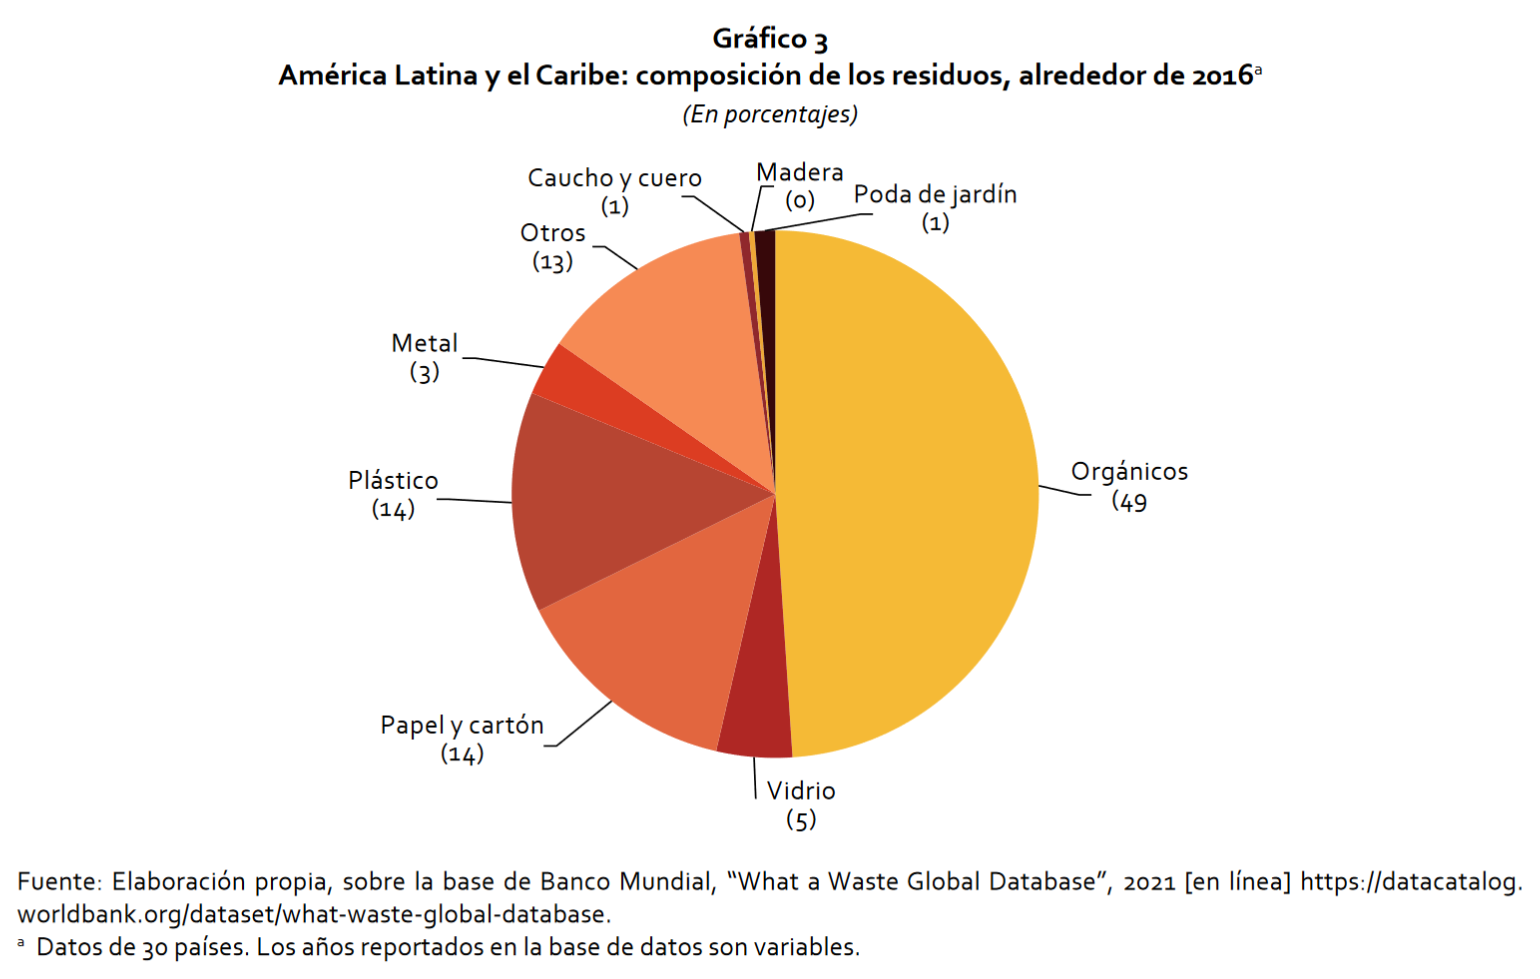
\includegraphics[width=1\textwidth]{../assets/waste-types-latam.png}
	\caption{Composición de los residuos sólidos urbanos en América Latina. Fuente: CEPAL, 2021.}
	\label{fig:waste-latam}
\end{figure}

\subsection{Residuos Orgánicos}
Los residuos orgánicos, como desechos de alimentos y residuos de jardinería, presentan oportunidades significativas para el compostaje y la producción de biogás. Sin embargo, su descomposición produce metano, un potente gas de efecto invernadero, si no se gestiona adecuadamente.

\subsection{Residuos Electrónicos}
Los residuos electrónicos contienen metales preciosos y ofrecen oportunidades económicas significativas. No obstante, su reciclaje presenta desafíos debido a la presencia de sustancias tóxicas, lo que requiere procesos de reciclaje especializados y costosos.

\subsection{Papel y Cartón}
El papel y el cartón son materiales reciclables y biodegradables, lo que los convierte en una opción sostenible. Sin embargo, la calidad del papel reciclado puede ser inferior a la del papel virgen, lo que limita su reutilización en ciertas aplicaciones.

\subsection{Plásticos}
El reciclaje de plásticos puede reducir la dependencia de los recursos fósiles y disminuir la contaminación. Sin embargo, la variedad de tipos de plástico y la contaminación cruzada pueden complicar los procesos de reciclaje, haciéndolos menos eficientes.

\subsection{Textiles}
El reciclaje de textiles apoya la sostenibilidad en la industria de la moda. A pesar de esto, la rápida moda contribuye a altas tasas de desechos textiles, y muchos de estos no son reciclables debido a mezclas de materiales y tratamientos químicos.

\subsection{Metales}
Los metales son altamente reciclables y su recuperación es eficiente en términos de energía. La principal desventaja es la posible degradación de la calidad con ciertos metales no ferrosos, lo que puede limitar su reutilización.

\subsection{Vidrio}
El vidrio es completamente reciclable y puede ser procesado infinitas veces sin pérdida de pureza o calidad. Sin embargo, la recolección y el transporte del vidrio deben manejarse con cuidado para evitar la contaminación y garantizar la viabilidad del reciclado.

Para ser reciclado, el vidrio debe ser separado por color y tipo, lo que puede ser un desafío en la gestión de residuos. Sin embargo, el vidrio reciclado tiene un alto valor en el mercado y puede ser utilizado para fabricar nuevos envases a menor costo.

\subsection{Residuos de Construcción y Demolición}
Estos residuos ofrecen un gran potencial de reutilización y reciclaje. El principal reto es la separación efectiva de los materiales en el sitio de demolición, lo cual es esencial para su posterior procesamiento.

\subsection{Decisión Final}
Para el alcance de este proyecto, se considerará entre plástico y vidrio debido a su relevancia (14\% y 5\% de la composición de residuos sólidos urbanos en América Latina, respectivamente) y potencial para la implementación de prácticas de economía circular. Se descarta la opción de residuos orgánicos debido a su alta generación de metano y la de residuos electrónicos por su complejidad en el reciclaje. Se descartan también textiles, metales y residuos de la construcción por su menor presencia en la composición de residuos sólidos urbanos en la región. Se descarta papel y cartón por su menor potencial de innovación en comparación con plástico y vidrio.
Se realizará un análisis más profundo de estos dos materiales para determinar cuál de ellos ofrece mayores beneficios y posibilidades de implementación efectiva en el contexto local.

\section{Comparación entre Vidrio y Plástico}

Para una adecuada selección de materiales en proyectos de economía circular, es crucial comprender las diferencias entre los tipos de residuos más comunes. A continuación se presenta una comparación detallada entre vidrio y plástico basada en varios criterios importantes para su gestión y reciclaje.

\begin{table}[h!]
\centering
\begin{tabular}{|l|c|c|}
\hline
\textbf{Criterio} & \textbf{Vidrio} & \textbf{Plástico} \\ \hline
Cantidad generada & 5\% & 14\% \\ \hline
Variedad de tipos & Baja & Alta \\ \hline
Usos comunes & Envases, ventanas, vajillas & Envases, muebles, electrónica \\ \hline
Complejidad de reciclaje & Baja & Alta \\ \hline
Impacto ambiental & Menor & Mayor \\ \hline
Tasa de reciclaje & Alta & Variable, generalmente baja \\ \hline
Degradación por reciclado & No degrada & Degradación de calidad \\ \hline
Requerimientos de tratamiento & Fundición a alta temperatura & Diversos métodos según tipo \\ \hline
Potencial de mercado para reciclados & Estable & Creciente pero complejo \\ \hline
\end{tabular}
\caption{Comparación entre vidrio y plástico en el contexto de economía circular.}
\label{tab:glass-vs-plastic}
\end{table}

Como se puede observar en la tabla \ref{tab:glass-vs-plastic}, el vidrio y el plástico presentan diferencias significativas en términos de cantidad generada, variedad, usos, y complejidad en su reciclaje. Mientras que el vidrio tiene una tasa de reciclaje relativamente alta y un impacto ambiental menor debido a su capacidad de ser reciclado múltiples veces sin pérdida de calidad, el plástico, aunque más versátil y utilizado en una variedad más amplia de productos, enfrenta desafíos significativos debido a su alta variedad y la degradación de calidad con cada ciclo de reciclado. Además, el impacto ambiental del plástico es considerablemente mayor, especialmente por su contribución a la contaminación marina y la dificultad de descomposición.

Debido a estas características, dentro del alcance de este trabajo se elige el vidrio como el material principal para la implementación de prácticas de economía circular en el contexto local. A pesar de su menor presencia en los residuos sólidos urbanos, el vidrio ofrece ventajas significativas en términos de reciclaje, impacto ambiental y viabilidad de mercado para los reciclados. 

El reciclaje del vidrio es especialmente relevante en la región de Mendoza, donde la industria vitivinícola es un pilar económico fundamental y el vidrio desempeña un papel crucial en la cadena de suministro de este sector. En esta región opera Verallia Argentina, una de las principales productoras de envases de vidrio del país. Esta empresa, siendo un actor esencial en la cadena de suministro del vidrio, juega un rol significativo en la promoción de la sostenibilidad dentro de la industria vitivinícola y en la economía regional. Actualmente, Verallia implementa prácticas de reciclaje de vidrio, proporcionando una base sólida para la adopción de tecnologías avanzadas y la mejora de los procesos de trazabilidad y gestión de residuos \cite{prodvidrio2024verallia}. A lo largo de este estudio, se explorará en profundidad cómo la cadena de suministro del vidrio en Verallia puede integrarse más efectivamente en la economía circular y cómo las innovaciones en el reciclaje de vidrio pueden maximizar su impacto ambiental y económico.

A lo largo de este trabajo se realizará un análisis más detallado de la cadena de suministro del vidrio y las oportunidades de innovación en el reciclaje de vidrio para maximizar su potencial en la economía circular.

\chapter{Entrevista a Verallia}
\label{cp:verallia-interview}

\parindent0pt

% TODO: redactar y formatear esta sección
% Bajar minuta de la entrevista con la chica de Verallia. Contar cuánto duró y lista de preguntas y respuestas, tipo de entrevista.

Para obtener una comprensión profunda de la situación del reciclaje de vidrio, particularmente en la provincia de Mendoza, se realiza una investigación de campo.
Como punto de partida, se lleva a cabo una revisión en internet de sitios web, artículos de diarios locales y boletines oficiales para documentar programas de reciclaje activos en la región y la presencia de empresas productoras relevantes.
A continuación, se realiza una entrevista semiestructurada con Lucía J., responsable del Área de Medio Ambiente de Verallia, la principal empresa productora de envases de vidrio en la región de Mendoza.
La entrevista se condujo de manera telefónica, utilizando preguntas guía predefinidas, pero con flexibilidad para explorar temas emergentes durante la conversación.
La conversación fue grabada con consentimiento previo y luego transcripta, complementándose con notas tomadas durante la entrevista.

---

Durante la etapa de investigación y recopilación de información para el desarrollo de este trabajo, luego de definir el alcance, se llevó a cabo una entrevista con una representante de Verallia, la principal empresa fabricante y manufacturadora de la fabricación de envases de vidrio en Mendoza, principal proveedora de la industria vitivinicola local.

La entrevista se realizó con Lucía, quien es parte del equipo de sostenibilidad de Verallia Argentina en Mendoza. Previo a la entrevista fue informada sobre el contexto de este trabajo y la finalidad de la entrevista y dio consentimiento para que la información compartida fuera incluida en este trabajo. 

La conversación se centró en conocer los procesos actuales de producción y reciclaje de vidrio en Verallia, las iniciativas sostenibles que la empresa está implementando y las oportunidades para mejorar la trazabilidad y la gestión de residuos en la cadena de suministro de la empresa.

La entrevista fue realizada por teléfono, tuvo una duración aproximada de 45 minutos y fue grabada. La modalidad de la entrevista fue semiestructurada, permitiendo una conversación fluida y la posibilidad de profundizar en temas relevantes a medida que surgían. Previo a la entrevista, se preparó una lista de preguntas que abarcaban los siguientes temas:

-
- 
-

A continuación se presenta un resumen de las preguntas realizadas y las respuestas obtenidas:

% Contarlo de forma fluida, no como lista de preguntas y respuestas.
Preguntas:
- Contame cómo es el proceso que hacen ustedes
- El vidrio reciclado de dónde sale
- Qué hacen cuando les llega el vidrio, viene clasificado o lo clasifican ustedes?
- Cómo se involucran sus clientes
- Hay alguna reglamentación o restricción para poder reciclar?
- Les serviría que el vidrio llegara en cantidad y preclasificado?
- Qué les interesaría de un sistema como este? Qué le serviría a tu empresa? Qué tanto les serviría un sistema de trazabilidad? Creen que sería factible incorporar un sistema de estas características?
- Cuánto vuelve en relación a lo que venden?
- Sabés si alguno de tus clientes tienen algún programa particular o compromiso con lo sustentable.

Respuestas:
Recolectores urbanos recogen vidrio.
No hay cultura de reciclado en Arg.
En el camion va junto y en la planta lo separan.
En otros paises hasta el usuario separa.
No hay una politica gral en Mza, es por cada municipio.
A ellos les vende el vidrio los recolectores en negro. Necesitan que sean en blanco. Tienen 2 empresas que cuando compran el vidrio lo limpian. La limpieza es manual y cara. Tienen su nueva propia planta de limpieza.
No se puede reciclar vidrios de distintos colores juntos.
V reciclan botellas y frascos. 
El vidrio limpio va directo a la linea de producción.

V accion transparente es puertas afuera y Lucia es puertas adentro. Hay 32 campanas de la acción trasparente. El muni retira y ellos compran y reciben.
Campañas de entradas al cine.
3 o 4 eventos al año. 
También fomentan que los empleados reciclen.
Concientizar y fomentar el reciclado.
Las campañas dan un aporte mínimo de vidrio.
No acompañan las políticas. 
Mucho viene de recicladores y pymes. Bodegas a veces traen poco y las campañas traen poco.
Sale más barato la materia prima que comprar y limpiar vidrio para reciclaje.
Intermediarios por los que están en negro.
Tienen que clasificar ellos. A veces descartan mucho por los altos niveles de plomo.
La planta de limpieza clasifica. Separan por color y por no sé qué más. Mati de reciclaje. Separan tapas etiquetas basura. No saben de dónde vienen. Competencia Katorini? 
Hay suficiente oferta
Cuál es la legislación para comprar vidrio? Es interna o internacional? Podría venir de greenly la entrega (centralizamos a los recicladores). Estilo punto verde.

Los clientes suyos querrían sumarse a una campaña? A ustedes les serviría? Vendría ya clasificado. Podrían hacerse convenios.

Cuánto fue el objetivo este año? Menor al del año pasado.


- Les serviría un sistema de trazabilidad?
- La empresa podría participar localmente de un experimento o no se puede?Sí
- Les ponen marcadores impresos a las botellas? Eso puede servir para después reciclar y pagás mejor tu vidrio.
- Qué nivel d trazabilidad tienen los envases? Tienen numero de molde y la marca abajo
- La limpieza siempre es necesaria antes re-usarse el calcín

\chapter{Viaje de Investigación}
\label{cp:europe-trip}

Aprovechando una oportunidad profesional, se realizó un viaje de investigación de dos semanas a Europa.
Durante este viaje, se visitaron y estudiaron sistemas de reciclaje y programas de incentivos de reciclaje en tres países europeos.
Las actividades incluyeron visitas a centros verdes, interacciones con organizaciones involucradas en el reciclaje, exploración de redes de comercios circulares u orientadas a la sustentabilidad, y encuentros con organizaciones dedicadas a promover la economía circular.
Los hallazgos y observaciones de este viaje, documentados a través de notas y fotografías, se detallan en el Apéndice.

---

En el mes de noviembre de 2024, durante la etapa de definición del alcance de este trabajo, oportuamente (por motivos profesionales ajenos a este trabajo) se realizó un viaje de investigación a Europa para conocer de primera mano los sistemas de reciclaje y economía circular implementados en diferentes países. Los resultados de esta experiencia resultaron ser enriquecedores para este trabajo de tesis, a pesar de haber generado un retraso en su planificación.

Este viaje tuvo como objetivo principal aprender sobre las mejores prácticas en la gestión de residuos y el reciclaje, así como explorar la viabilidad de implementar un sistema similar en ciudades de latinoamérica. A continuación, se detallan los aspectos más relevantes de la experiencia:

- Se visitaron 3 ciudades: Madrid (España), Amsterdam (Países Bajos) y Berlín (Alemania), cada una con sus propios sistemas de reciclaje y gestión de residuos.

- En Madrid, no tienen DRS, se observó la mecánica de recolección diferenciada y las categorías de recolección en origen. Se concluyó que entre los países visitados, España es el que menos ha avanzado en la implementación de sistemas de reciclaje y economía circular. A su vez, cabe destacar que la sustentabilidad y economía circular sí es un tema de interés y preocupación en la sociedad española, pero aún no se han implementado sistemas de recolección diferenciada ni DRS. España ha implementado la Ley REP hace algunos años y en 2025 se comenzó el plan para la implementación de DRS debido a que no alcanzaron sus metas de reciclaje de los últimos años.

- En Amsterdam se usa el sistema DRS, donde los consumidores pagan un depósito por las botellas de vidrio y plástico y latas, que se les devuelve al devolverlas en una RVM, ubicadas en las principales cadenas de supermercados. Con esta técnica se fomenta el hábito de reciclaje de envases en los ciudadanos, al incluirlo como un paso extra al proceso de ir de compras al supermercado. Este sistema ha demostrado ser efectivo para aumentar las tasas de reciclaje y reducir la cantidad de residuos. El problema hallado es que en la ciudad, los tachos de basura son vandalizados por recolectores informales para buscar botellas y latas (quienes usan el dinero obtenido para poder comprar comida diariamente), lo que genera un problema de higiene. Tuvimos la oportunidad de visitar un centro verde, y descubrimos que en esta ciudad las altas tasas de recuperación y reciclaje no se reduce a los envases, sino que también se aplica a otros tipos de residuos como papel, cartón, metales, electrodomésticos y muebles. En este centro verde se reciben los residuos reciclables y se clasifican para su posterior reciclaje. Es lo normal para los cuidadanos dirigirse a estos centros para entregar sus residuos o muebles y electrodomésticos en desuso. Respecto a la recolección diferenciada, se observó que los ciudadanos separan sus residuos en diferentes contenedores ubicados en la vía pública, y la recolección se realiza de manera semanal, de a un material por vez. Cada material se recoge una vez por semana. Los vecinos reclaman que la frecuencia de recolección es insuficiente, ya que los tachos se llenan rápidamente y no hay espacio para más residuos, que quedan expuestos en la vía pública junto a los contenedores. Es notorio que los ciudadanos contemplan el reciclaje como parte de su rutina diaria, y la separación de residuos es una práctica común. Además, se observó que los ciudadanos están muy concientizados sobre la importancia del reciclaje y la reducción de residuos. A su vez, se intentó indagar con el destino final de los residuos reciclables, y se nos informó que la mayoría de los materiales reciclables son procesados en el país, pero que son exportados a otros países fuera de europa para su disposición final y se desconoce el destino final de los mismos o si realmente son reciclados.

- En Alemania


En orden de evolución 
Contar la experiencia de investigación de sistemas de reciclaje en Europa. Contar sobre los DRS y los centros de reciclaje. Adjuntar fotos. Contar cada paso a paso qué cosas hicimos y a qué lugares fuimos. Hacer minuta.

\chapter{User Flow}
\label{cp:user-flow}

\parindent0pt

Contar el flujo de uso de la aplicación con screenshots de las pantallas y casos de uso de cada usuario. 

\chapter{Resultados de Pruebas Automatizadas}
\label{cp:automated-tests-execution}

Detallar para cada repositorio la lista de los títulos de las pruebas unitarias (son alrededor de 600 pruebas entre todo). 

Detallar también la lista de casos de prueba de tests de integración.

Detallar la lista de pruebas manuales realizadas.

Contar la lista de bugs levantados y resueltos o desestimados.

\chapter{User Acceptance Testing}
\label{cp:user-acceptance-testing}

\parindent0pt

Detallar la lista de pruebas manuales realizadas por los testers voluntarios, bugs levantados y resueltos, Adjuntar fotos del proceso.


%%% Annexes: Work that *YOU DID NOT* Develop %%%
% \addtocontents{toc}{\protect\contentsline{chapter}{Anexos}{}{}}

\setcounter{chapter}{11} % To start at the "L" chapter.
\MediaOptionLogicAnnexes
\begin{center}
    \crimsonfont
    \thispagestyle{empty}
        
    \vspace*{\fill}
    {\LARGE\fontsize{26}{26}\selectfont\textcolor{maincolor}{Anexos}\par}
    \vspace*{\fill}
\end{center}
\MediaOptionLogicBlank

% \chapter{Showcasing the First Annex}
\guideinfo{Annexes are supplementary sections in a dissertation that provide additional information or external documents not essential to the main arguments but that support or complement the research. Unlike appendices, \textbf{annexes generally contain material that was not developed by the author}, such as reports, legal documents, or published datasets from external sources. This information is placed separately to keep the main content concise, allowing readers access to relevant external references without disrupting the dissertation's flow.}

%%% Bibliography %%%
\renewcommand{\refname}{Bibliografía}
\printbibliography[title={\refname},heading=bibintoc]

%%% Print: Glossary and Acronyms %%%
\glossarytoc\printnormalglossary
\acronymtoc\printacronymglossary

%%% Back Page %%%
\ifthenelse{\equal{\MediaOption}{paper}}{\blankpage}{}

\clearpage
\null
\thispagestyle{empty}

% TODO: choose backpage background image/color.

% Back page

       \newcommand\BackgroundPicBackPage{%
    \put(0,0){%
    \parbox[b][\paperheight]{\paperwidth}{%
    \vfill
    \centering
    
\includegraphics[width=\paperwidth,height=\paperheight,keepaspectratio]{Figures/Theme/Back-Page-BG.pdf}%
    \vfill
    }}}


\AddToShipoutPictureBG*{\BackgroundPicBackPage}

\newgeometry{margin=1.98cm, top=1.47cm, bottom=1.47cm}
\noindent\clearpage
\restoregeometry


\end{document}
